% Dedicated HR feature pages. Shared source for HTML, PDF and Word.
% Each page: what it is, path, screenshot, what you record (every tab), what you can do, diagram, steps and check.

\clearpage
\section{Members}
\label{sec:hr-feature-members}

A member is a person who works in the organization. The record is a full employee file: from identity and contact to qualifications and bank account. An assignment links the member to a job.

\textbf{When is it useful?} One record for Sarah for her whole time at work; her job changes, her file stays. \textbf{Open:} HR / Workforce / Members.

\begin{figure}[H]
\centering
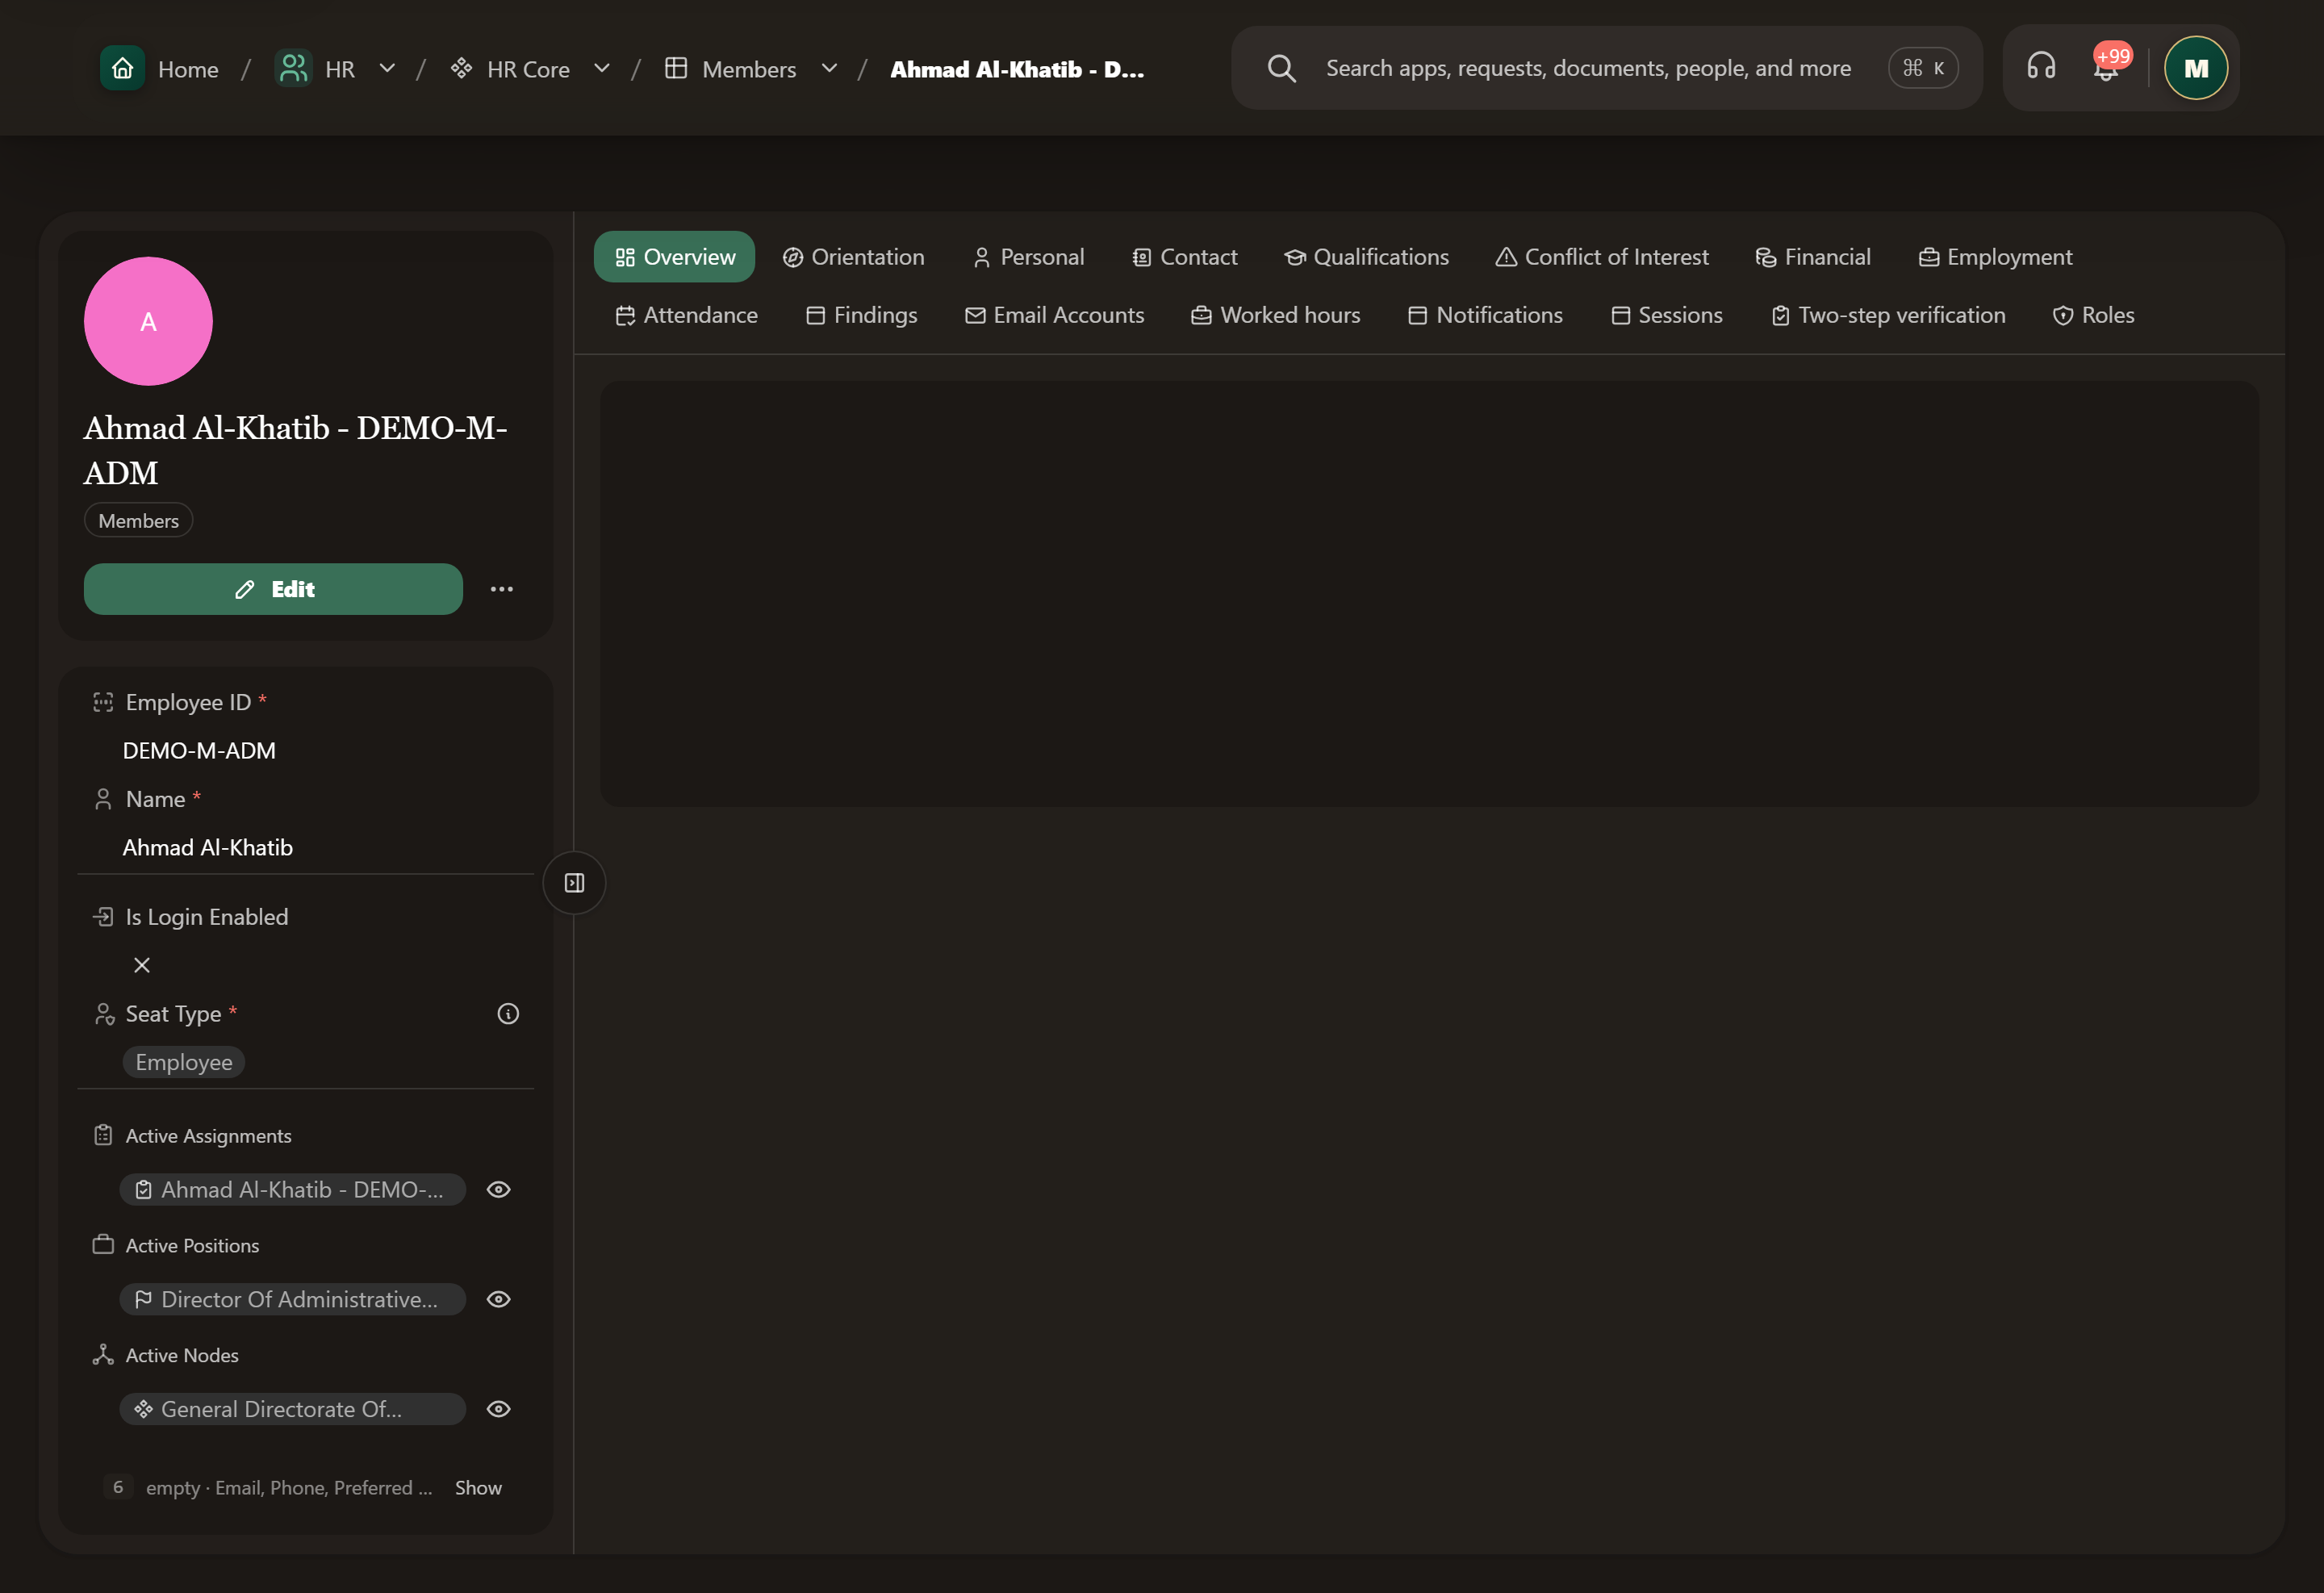
\includegraphics[width=0.95\linewidth]{figures/screens/ch02-member-fields-en.png}
\caption{Members: demo employee record; separate from the Sarah example}
\label{fig:hr-feature-members-screen}
\end{figure}

\begin{table}[H]
\centering
\caption{What do you record in a member file?}
\label{tab:hr-feature-members-data}
\rcZebra
\begin{tabularx}{\linewidth}{R{3.6cm} Y}
\rcHeaderRow
\thh{Tab or section} & \thh{What do you add?}\\
Main details &Employee ID \req{} and Name \req{}, email, phone and photo, login enabled, preferred language and timezone, fingerprint ID.\\
Personal & Father and mother name, gender, marital status, blood type, birth date and place, nationality, national ID and file, CV, passport, driver license, family members.\\
Contact & Address and address file, personal, work and home phones, personal and work email, emergency contacts.\\
Qualifications & Educations, skills and proficiency, languages, trainings, past experiences, with their certificates.\\
Conflict of Interest & Relatives in the organization, another workplace, supplier or shareholder conflicts, and the review decision and status.\\
Financial & Bank accounts, employee insurance, bonuses and deductions, salary slips.\\
Employment, Attendance & The member's assignments, leave balances, leaves.\\
Account tabs & Email Accounts, notifications and quiet hours, sessions, two-step verification, linked devices when enabled.\\
\end{tabularx}
\end{table}

These are the system's default fields; your organization's administrator may change them. Active positions and nodes are filled by the system \gen{} from assignments.

\subsection{What can you do?}

\begin{itemize}
  \item “Add Assignment” from the member file, with the member already selected.
  \item “Change password”, with “Require password change on next login”.
  \item “Offboard member”: choose “Transfer” to a successor, “Unassign” or “Preserve” for their responsibilities, set the effective date, and review what is affected.
  \item The list: cards for total members, members with active assignments and members without.
\end{itemize}

\begin{figure}[H]
\centering
\begin{tikzpicture}[node distance=0.5cm,stepBox/.append style={minimum width=6.5cm,text width=6.1cm,minimum height=0.8cm}]
  \node[stepBox] (a) {Sarah's record};
  \node[stepBox,below=of a] (b) {Job assignment};
  \node[stepBox,below=of b] (c) {Review job\\and period};
  \draw[flowsTo] (a) -- (b);
  \draw[flowsTo] (b) -- (c);
\end{tikzpicture}
\rclegend
\caption{Steps of use; arrows do not mean automatic processing}
\label{fig:hr-feature-members-flow}
\end{figure}

\subsection{Try it and check}

\begin{enumerate}
  \item Open Members and search for Sarah before adding a record.
  \item Add Employee ID 0001, the name “Sarah Al-Khatib” and an email, then “Save”.
  \item Open the “Contact” tab and add an emergency contact with name, phone and relationship, then save.
  \item From the record menu choose “Add Assignment” and link her to her position.
\end{enumerate}

\textbf{Check:} reopen the record and review the tabs. Her job appears under “Employment” once the assignment is saved.

\subsection{Employee record tabs}

\begin{figure}[H]
\centering
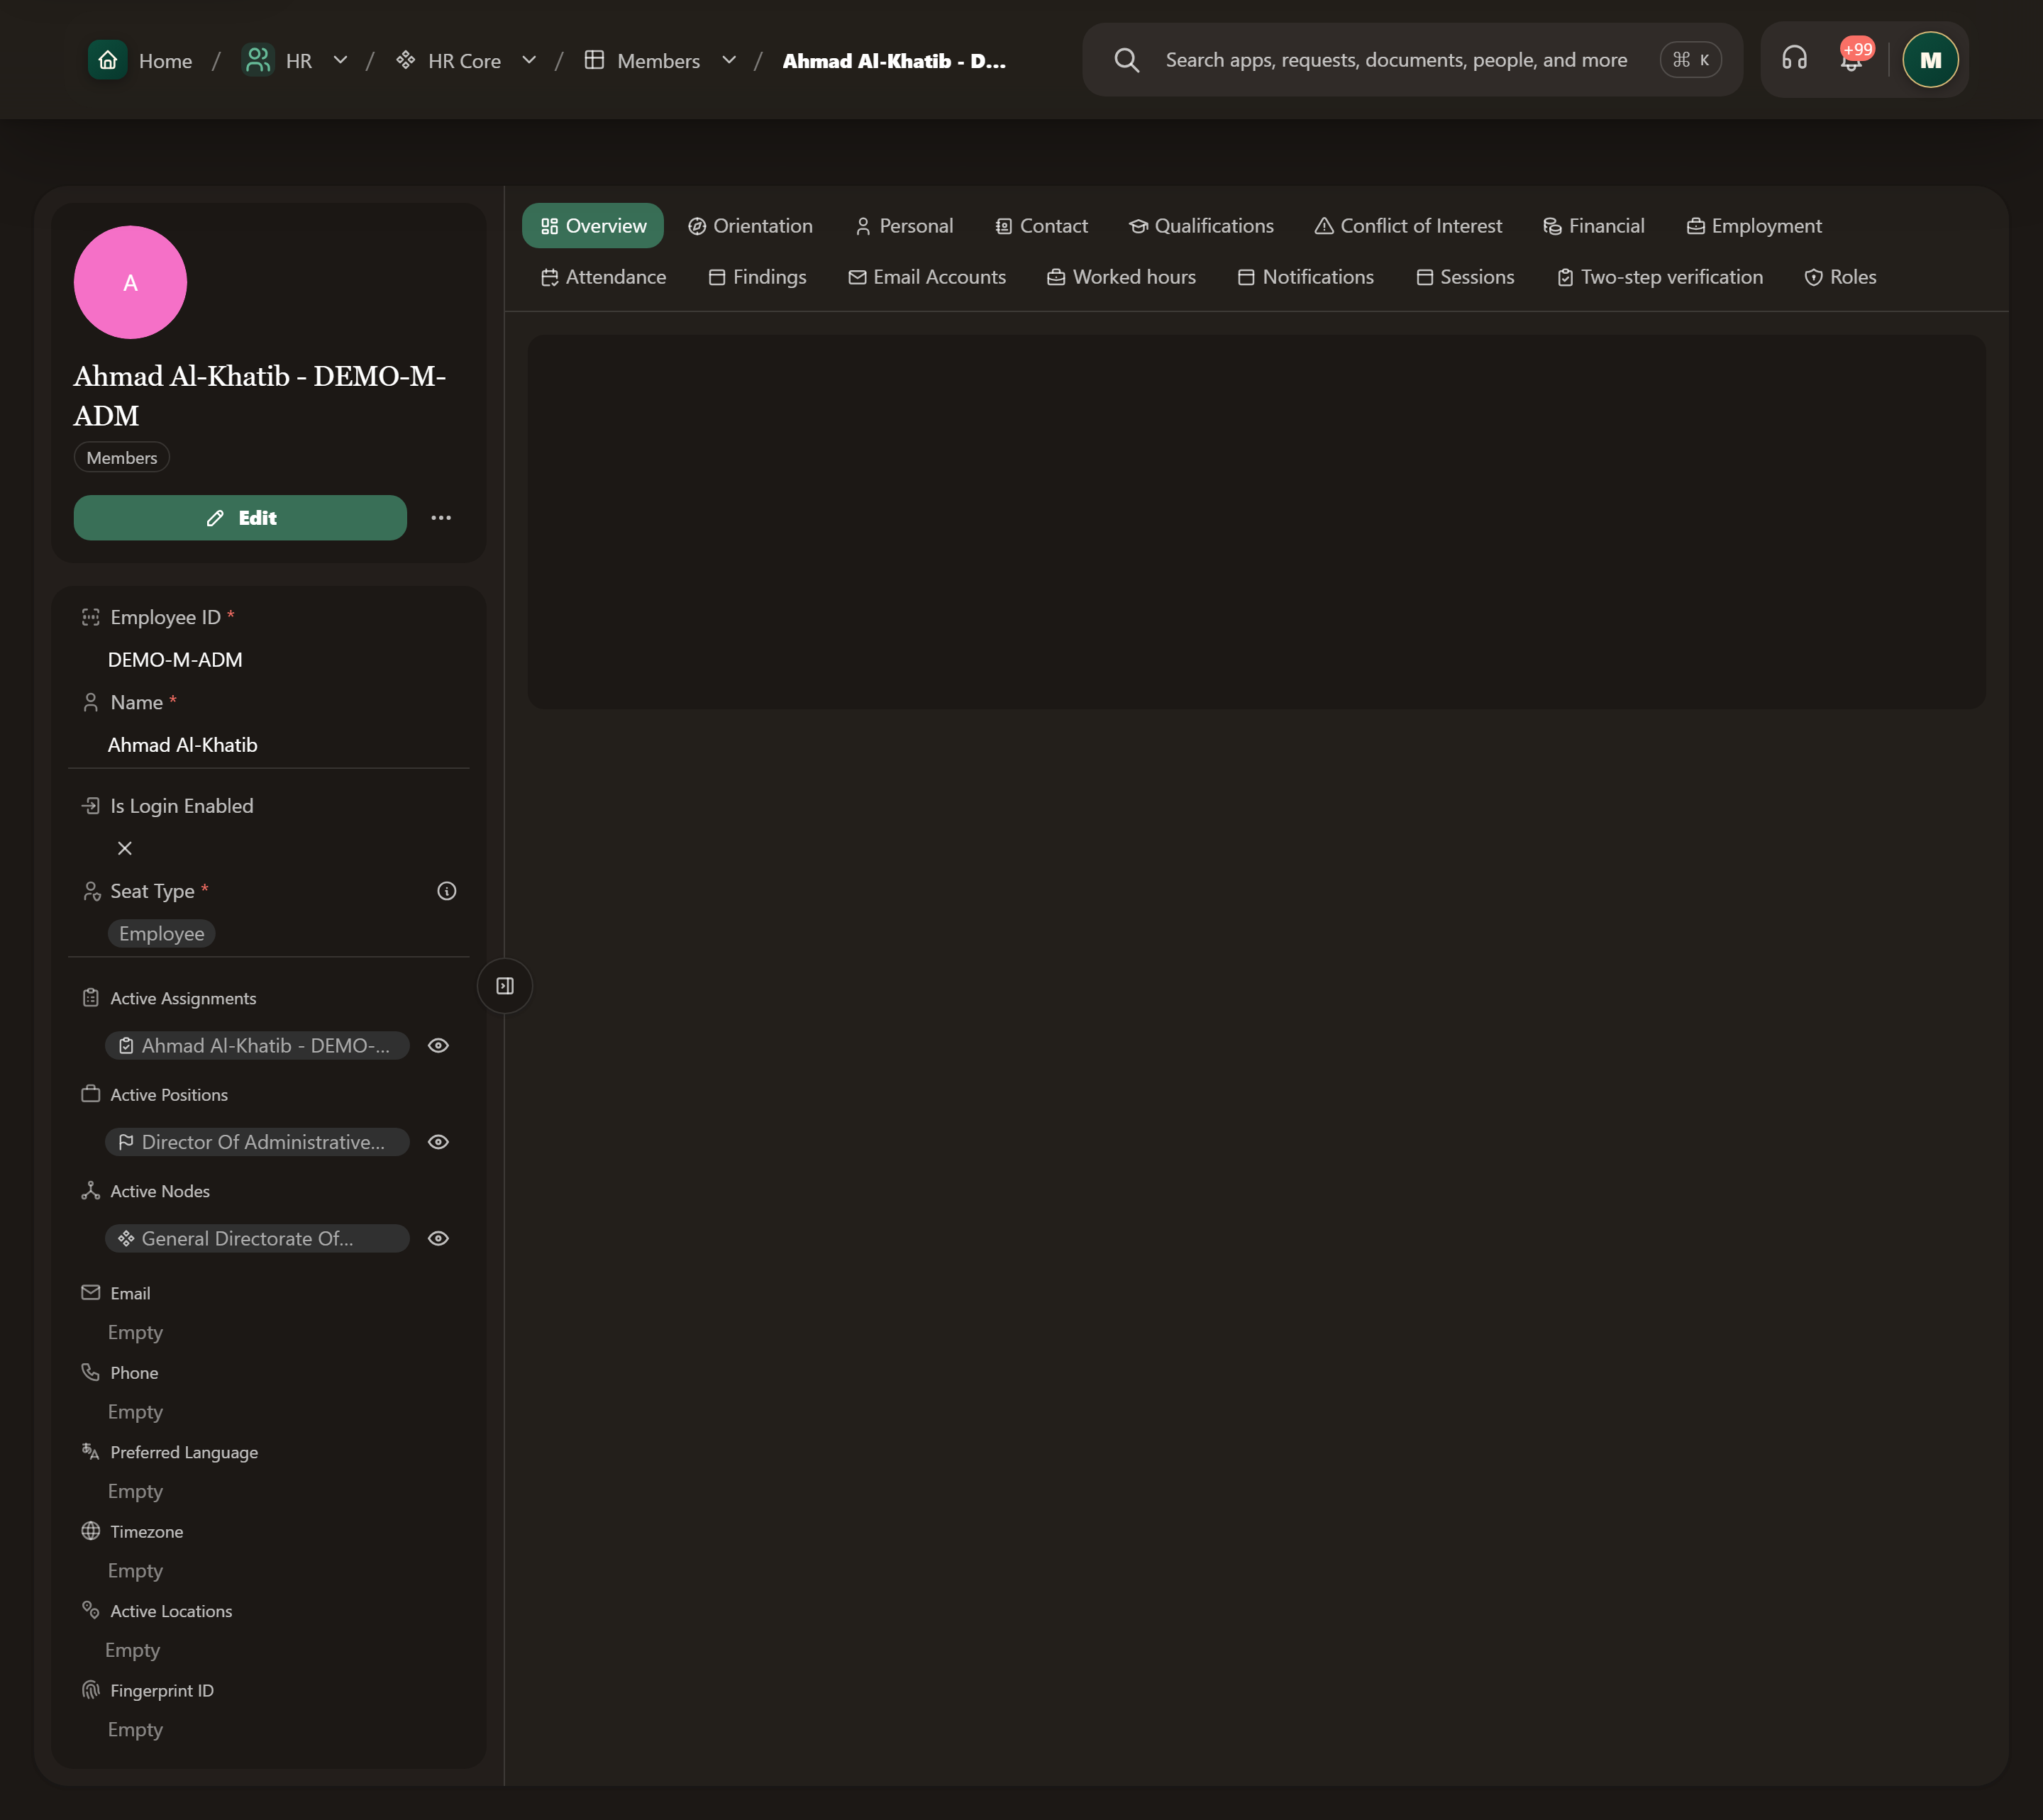
\includegraphics[width=0.95\linewidth]{figures/screens/ch03-member-tab1-en.png}
\caption{Demo employee record — Overview tab}
\label{fig:hr-member-tab1}
\end{figure}

\begin{figure}[H]
\centering
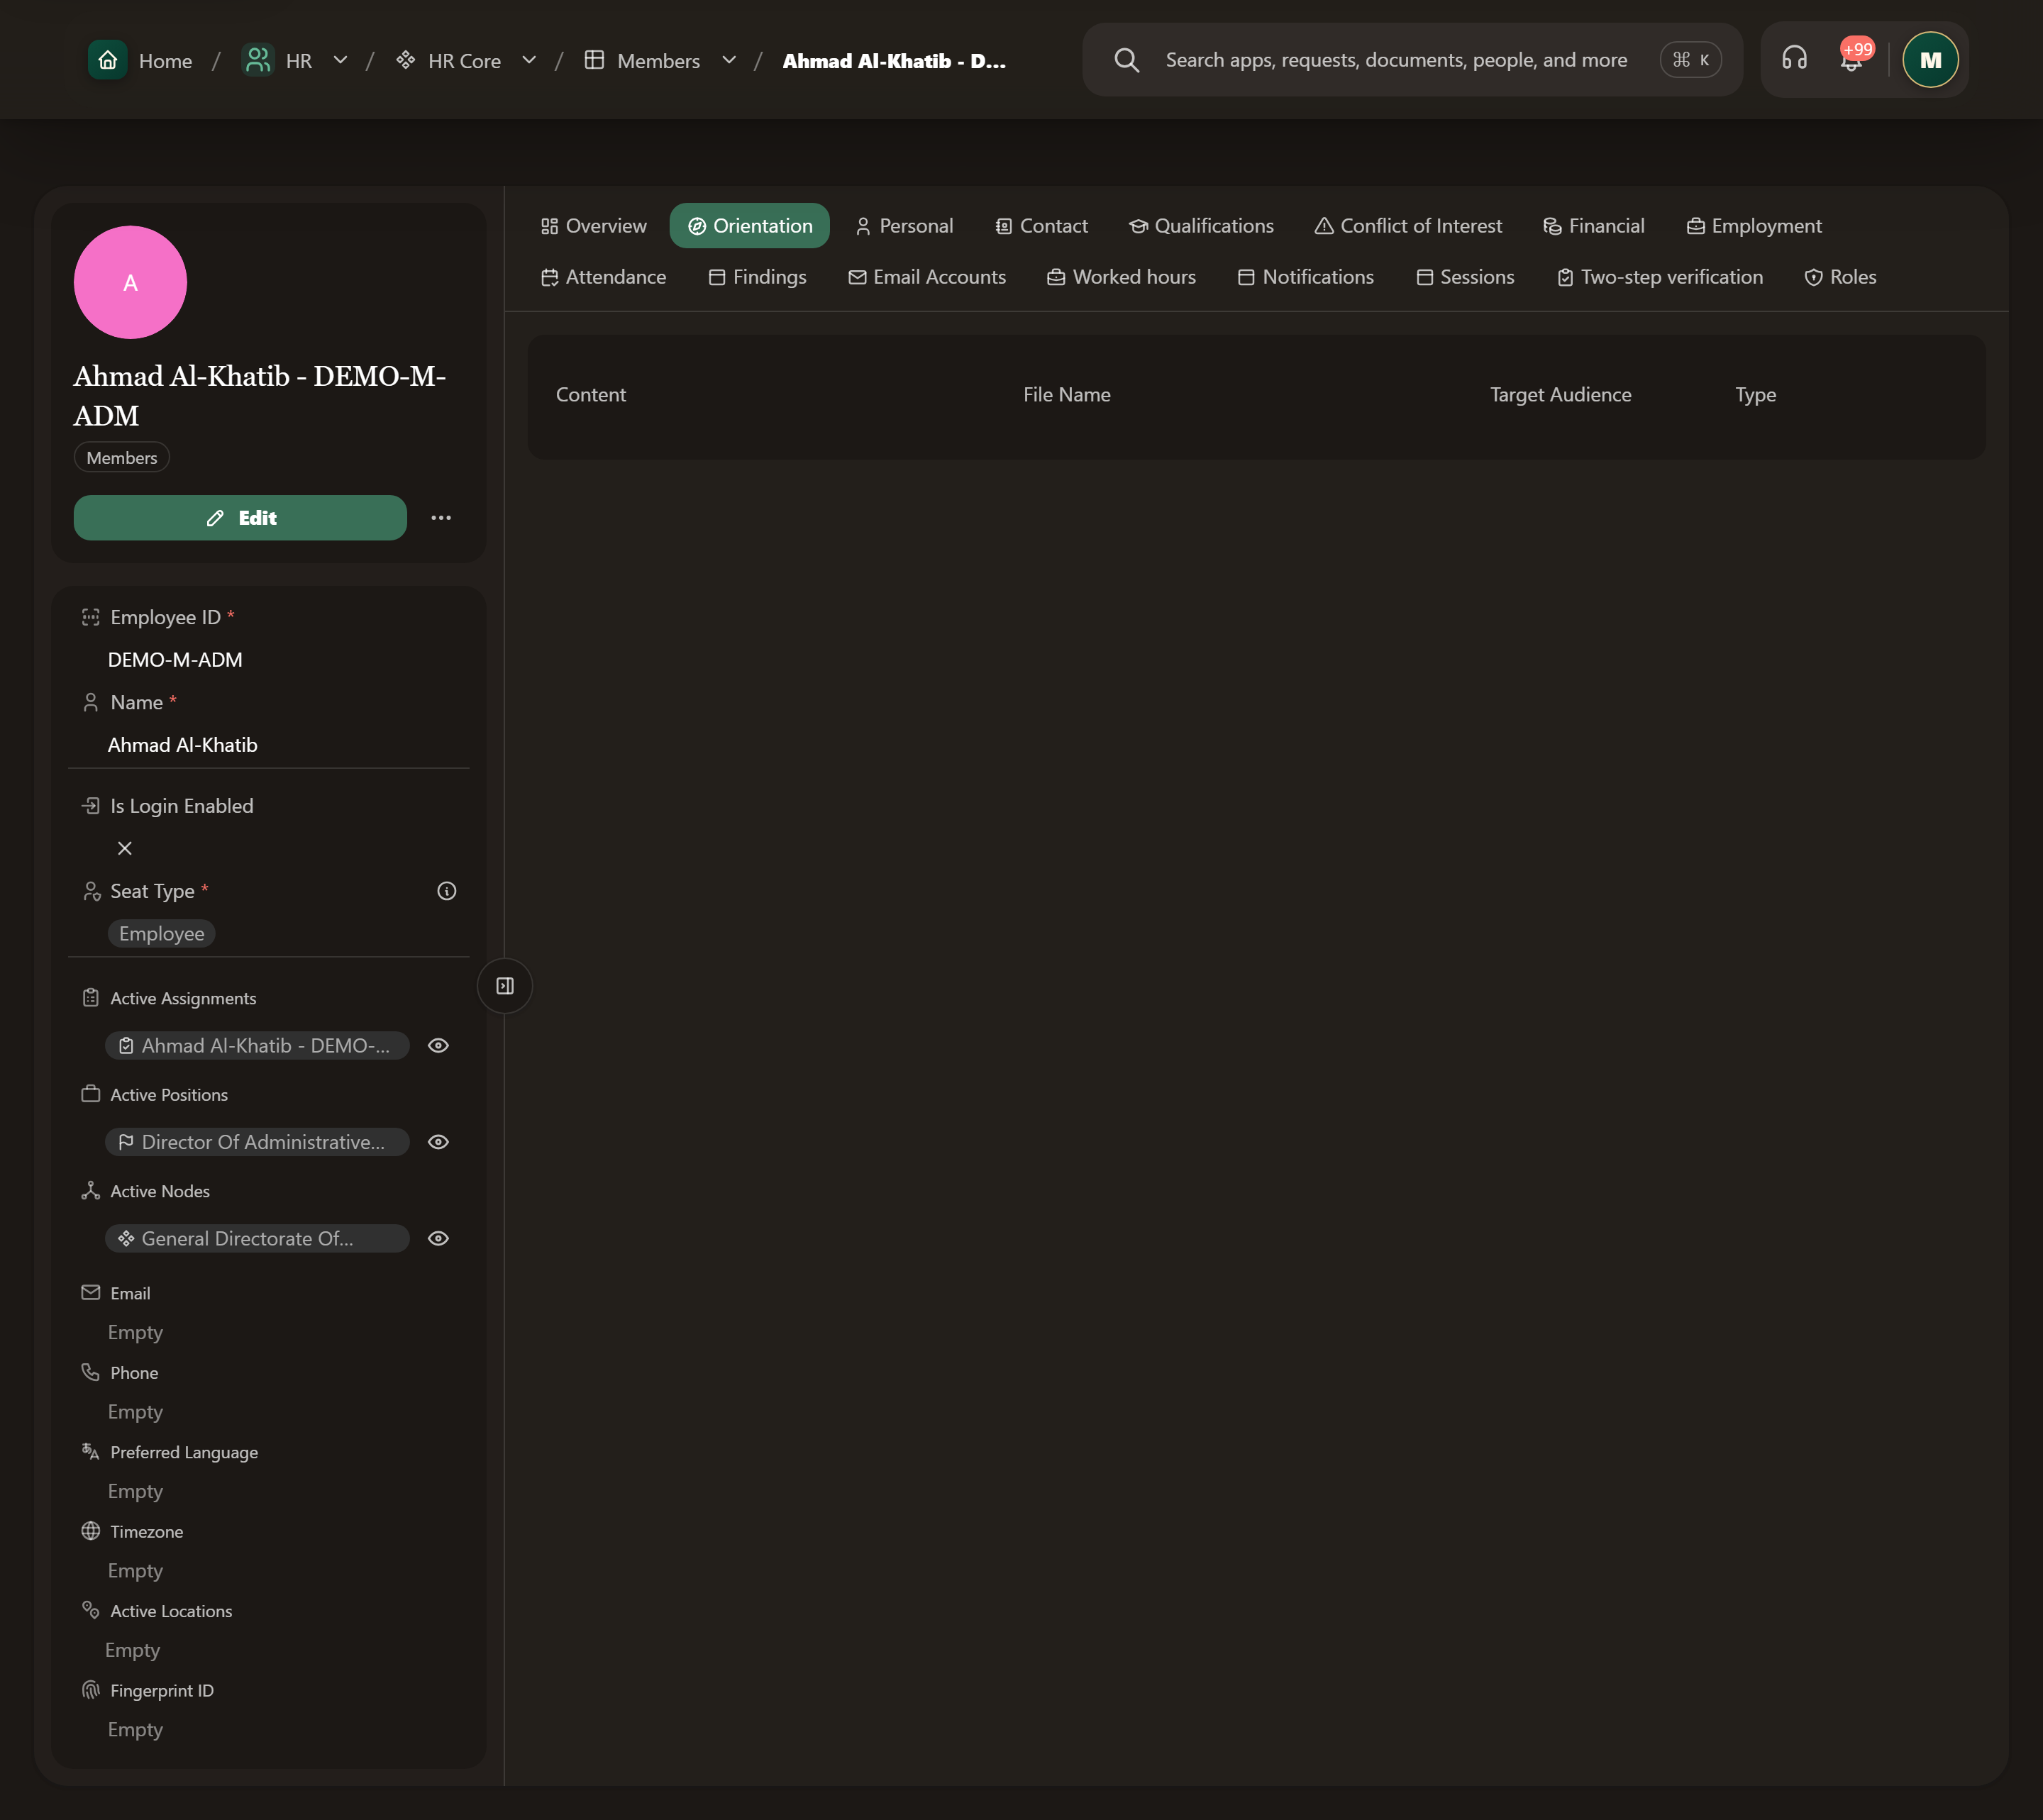
\includegraphics[width=0.95\linewidth]{figures/screens/ch03-member-tab2-en.png}
\caption{Demo employee record — Orientation tab}
\label{fig:hr-member-tab2}
\end{figure}

\begin{figure}[H]
\centering
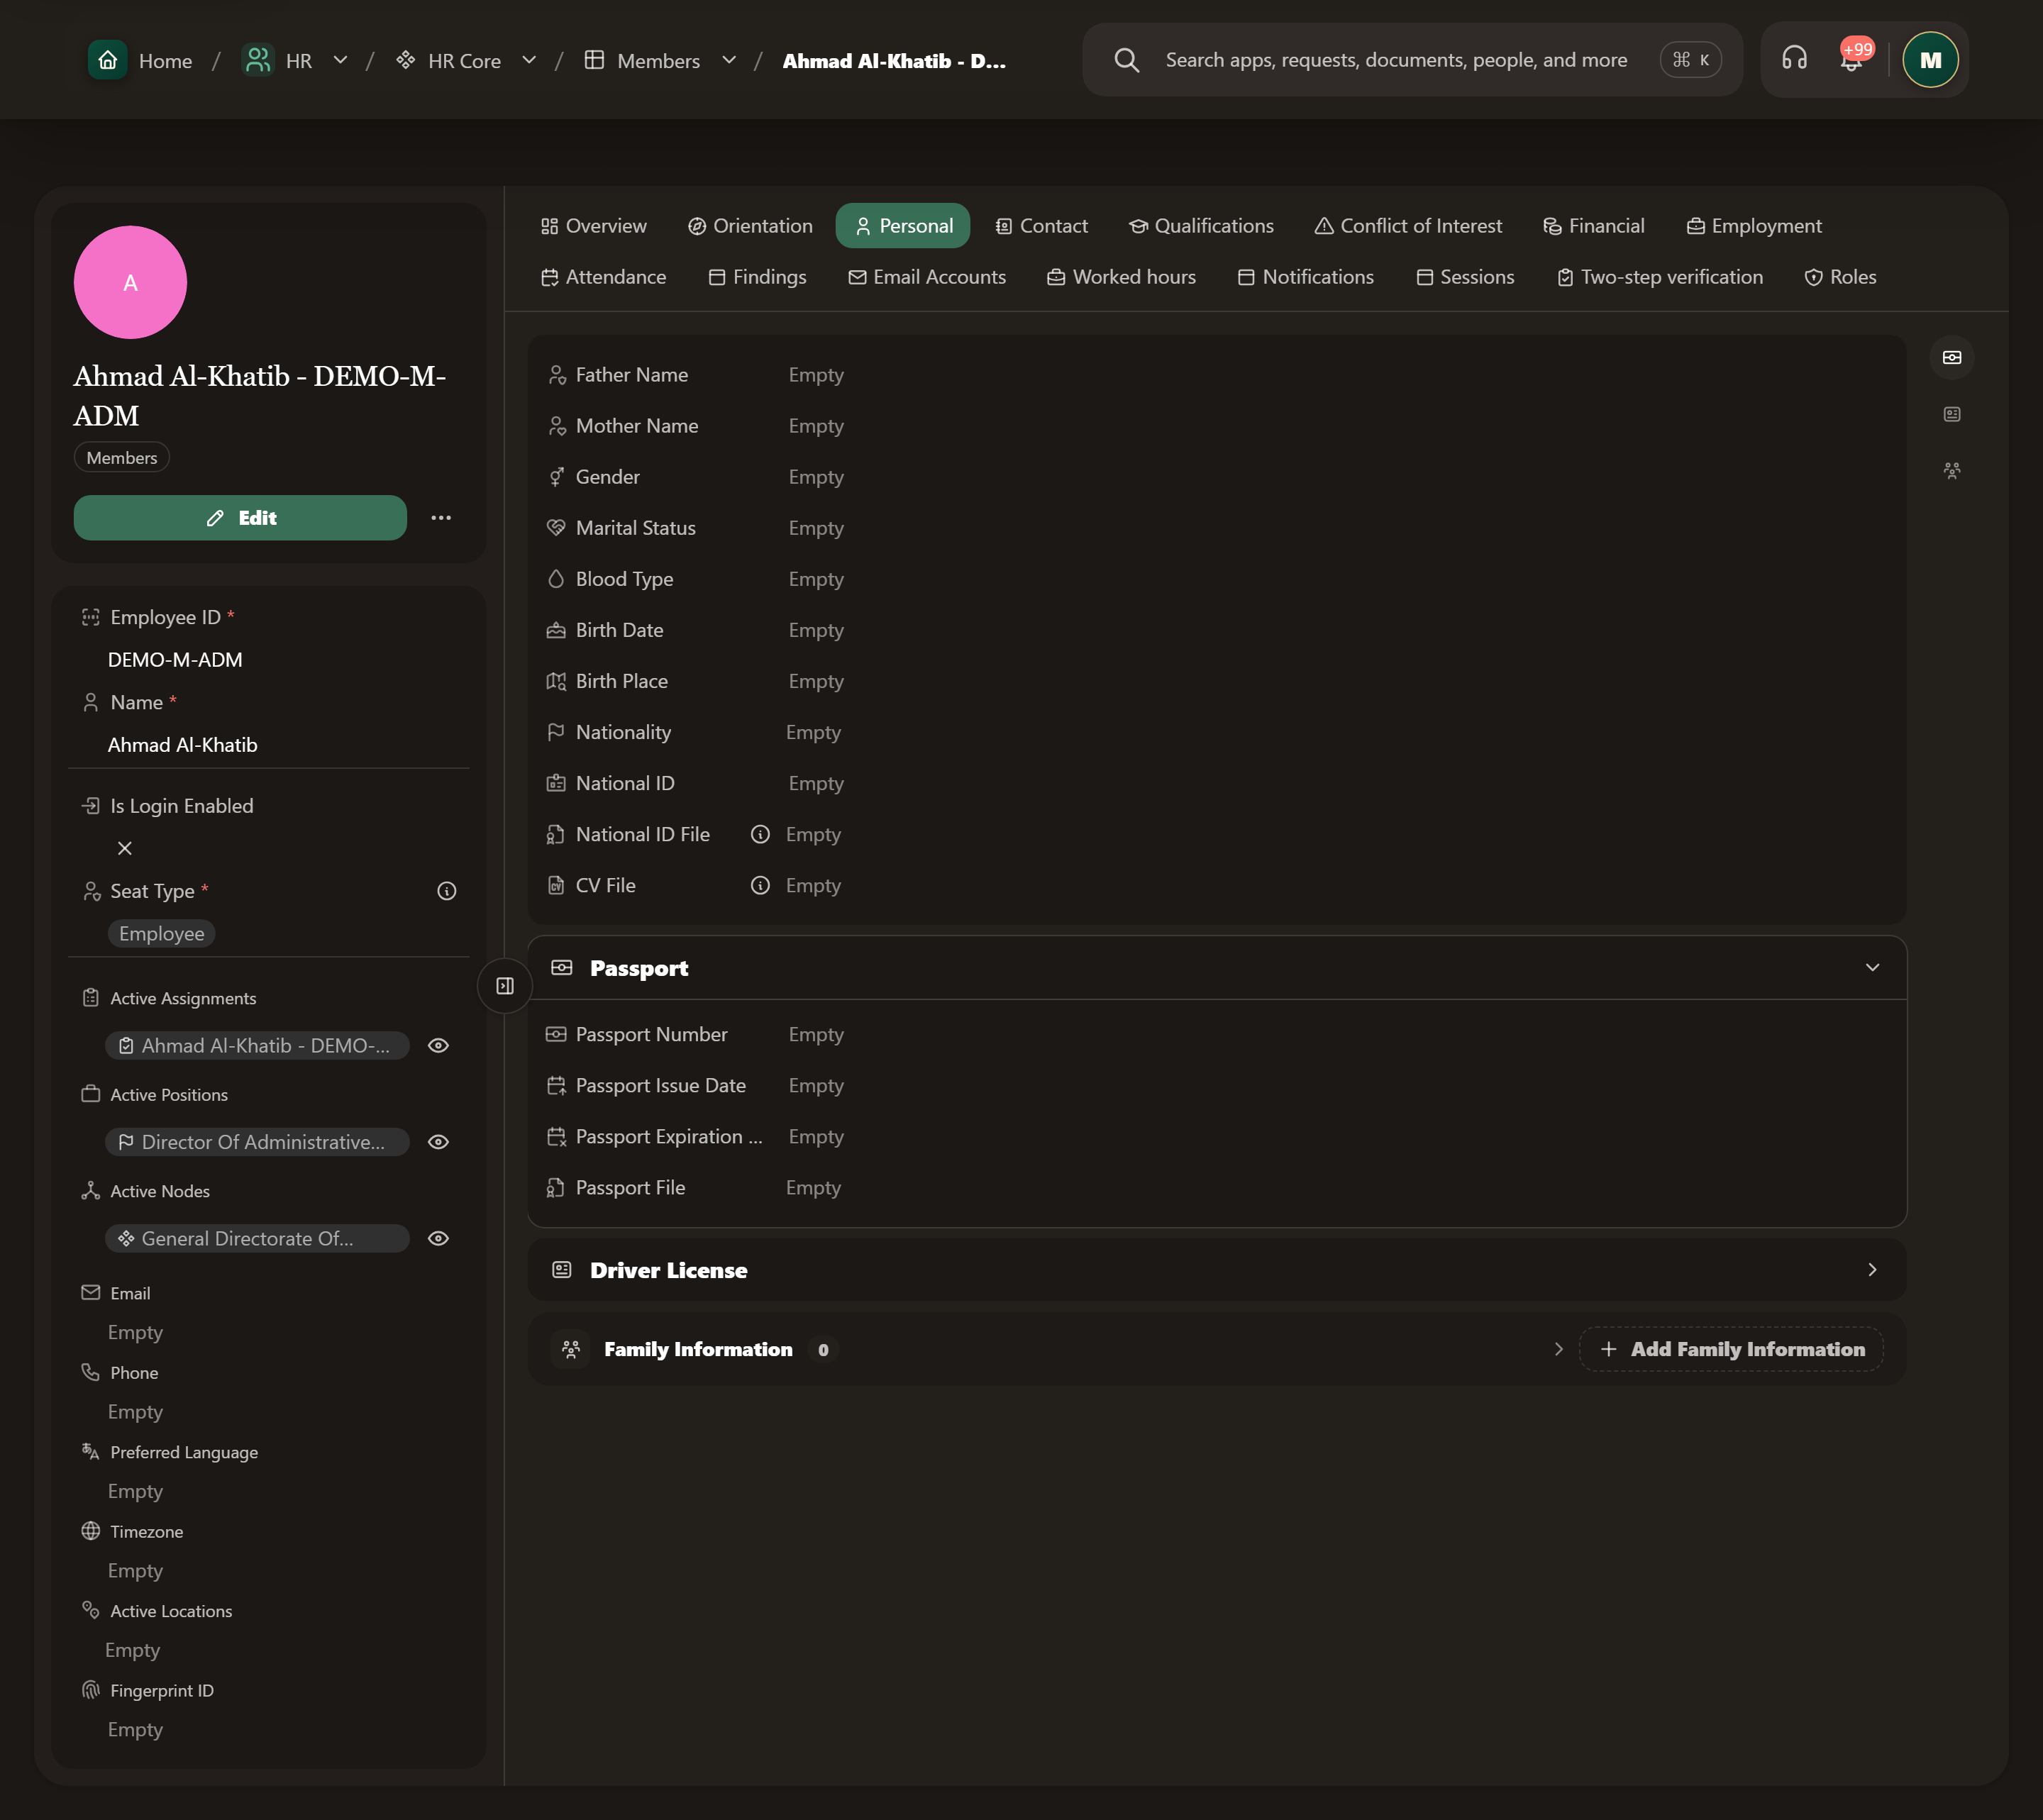
\includegraphics[width=0.95\linewidth]{figures/screens/ch03-member-tab3-en.png}
\caption{Demo employee record — Personal tab}
\label{fig:hr-member-tab3}
\end{figure}

\begin{figure}[H]
\centering
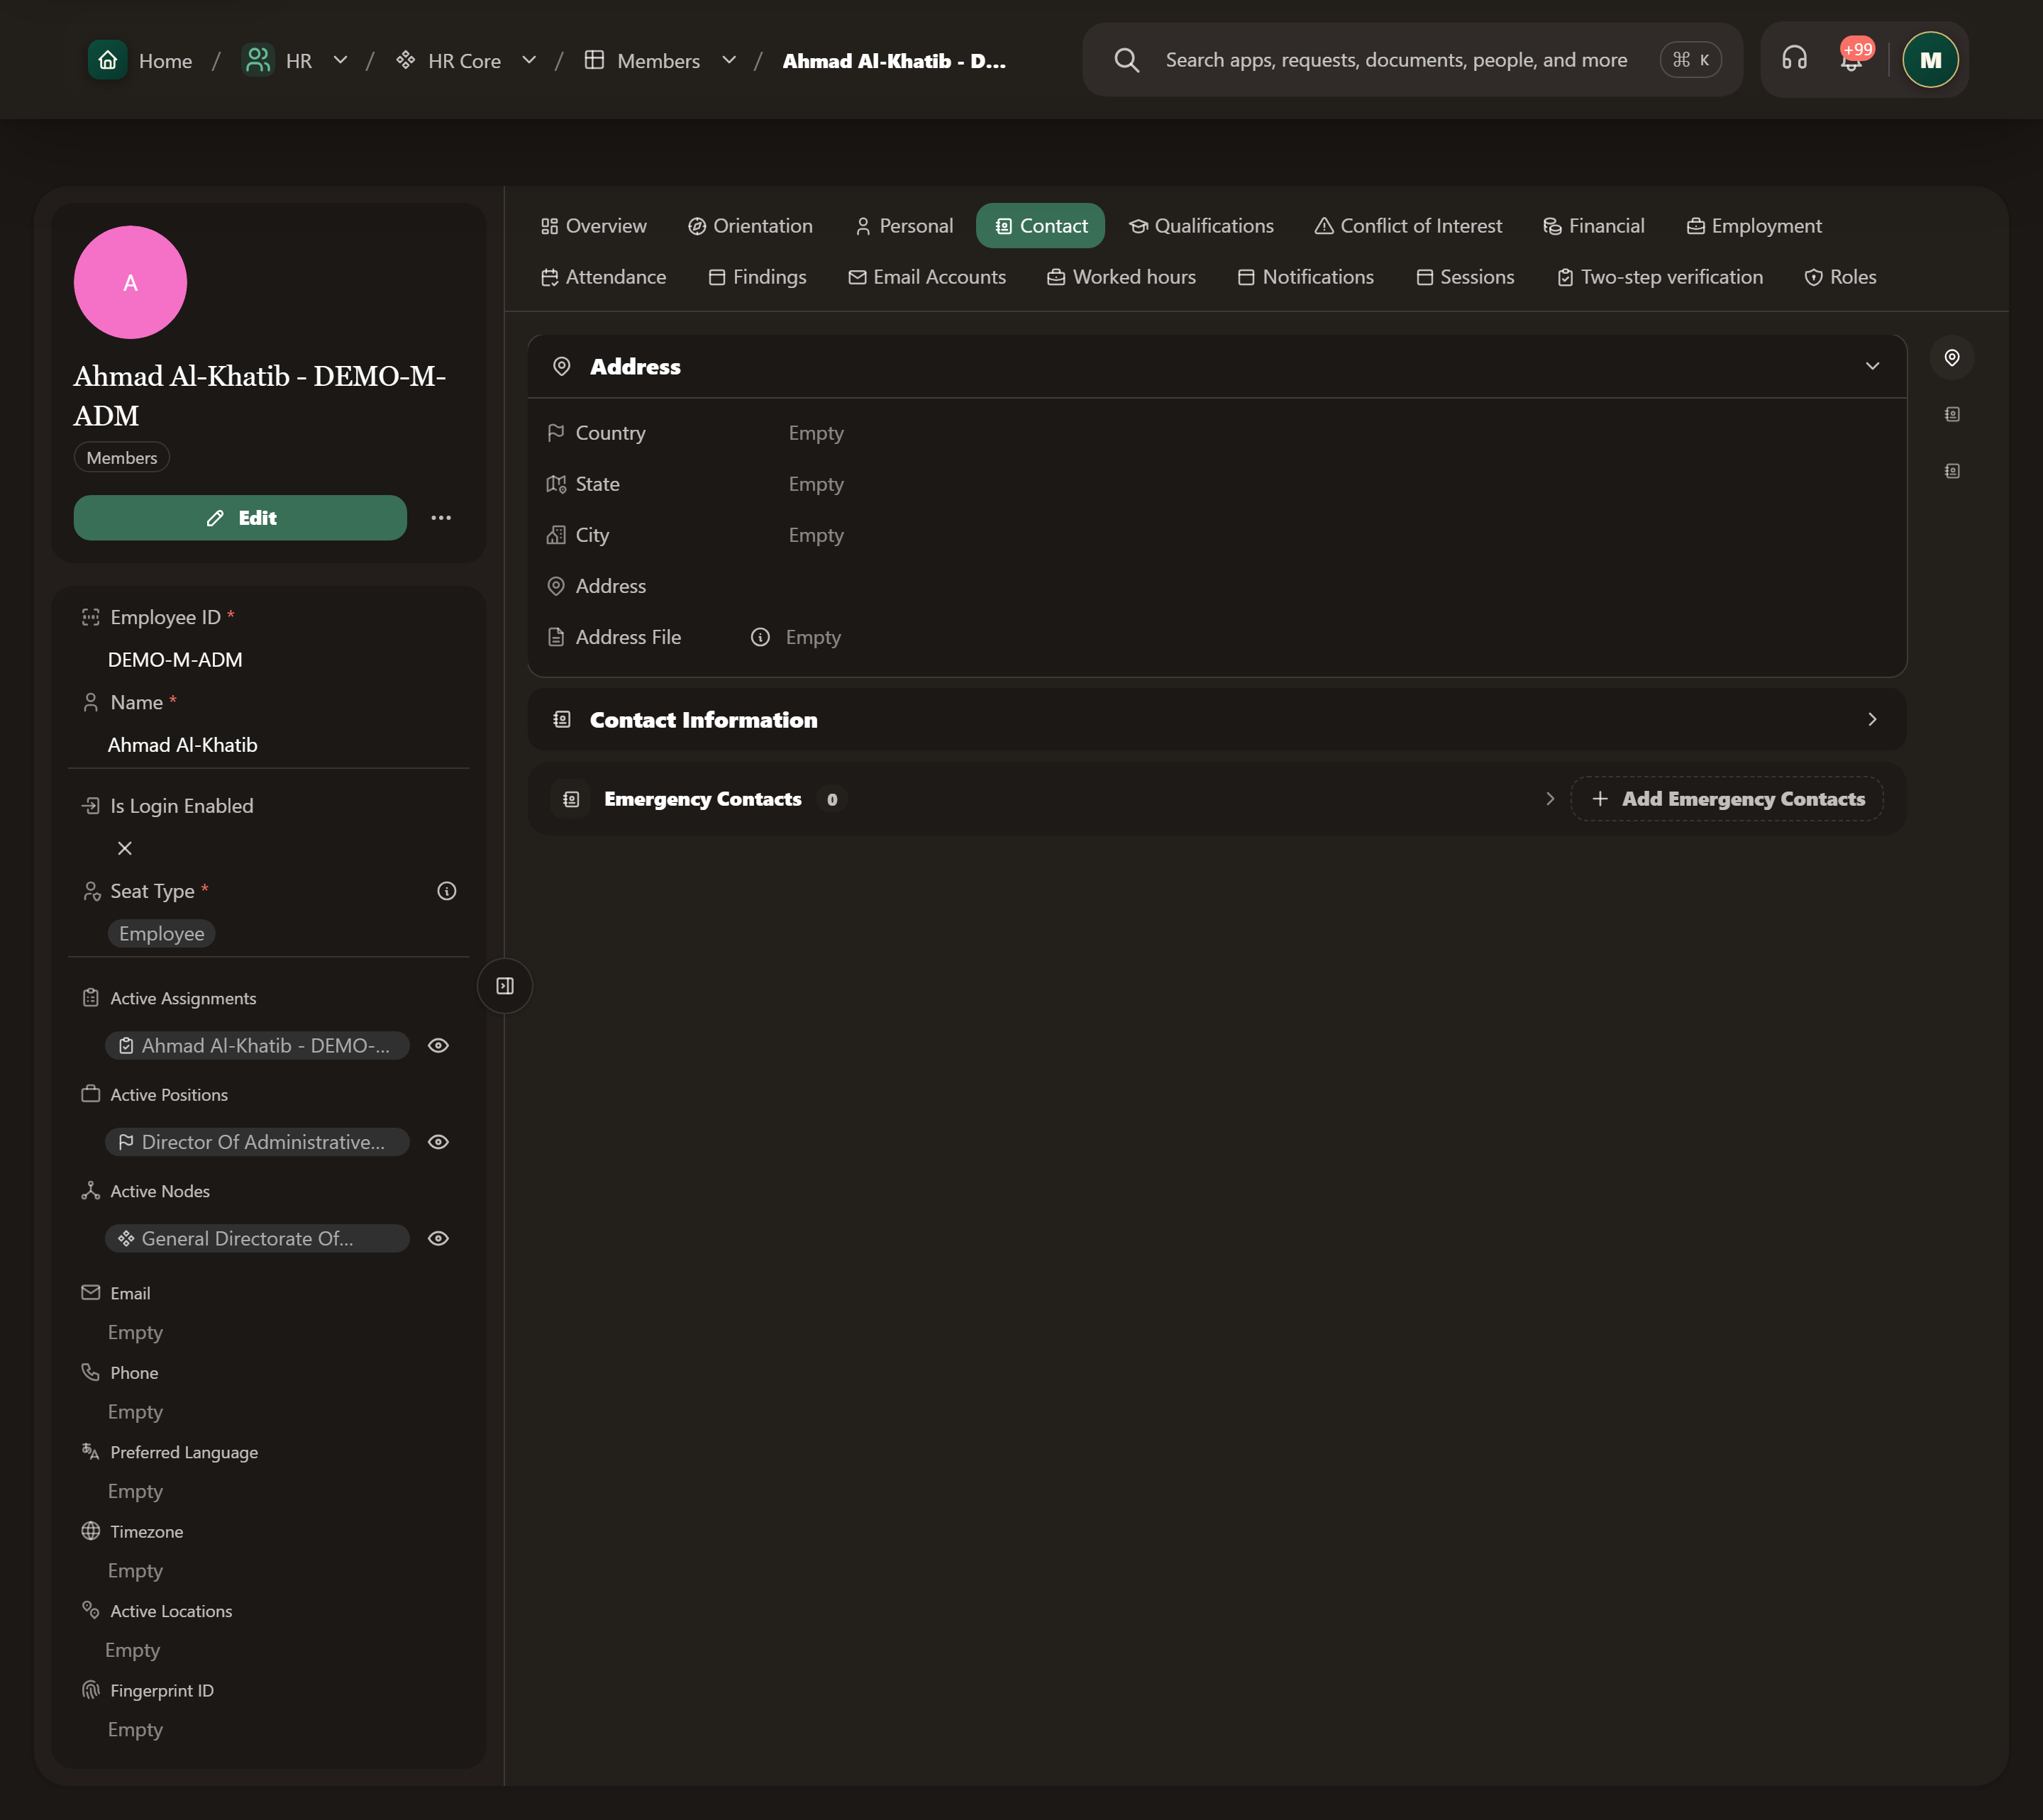
\includegraphics[width=0.95\linewidth]{figures/screens/ch03-member-tab4-en.png}
\caption{Demo employee record — Contact tab}
\label{fig:hr-member-tab4}
\end{figure}

\begin{figure}[H]
\centering
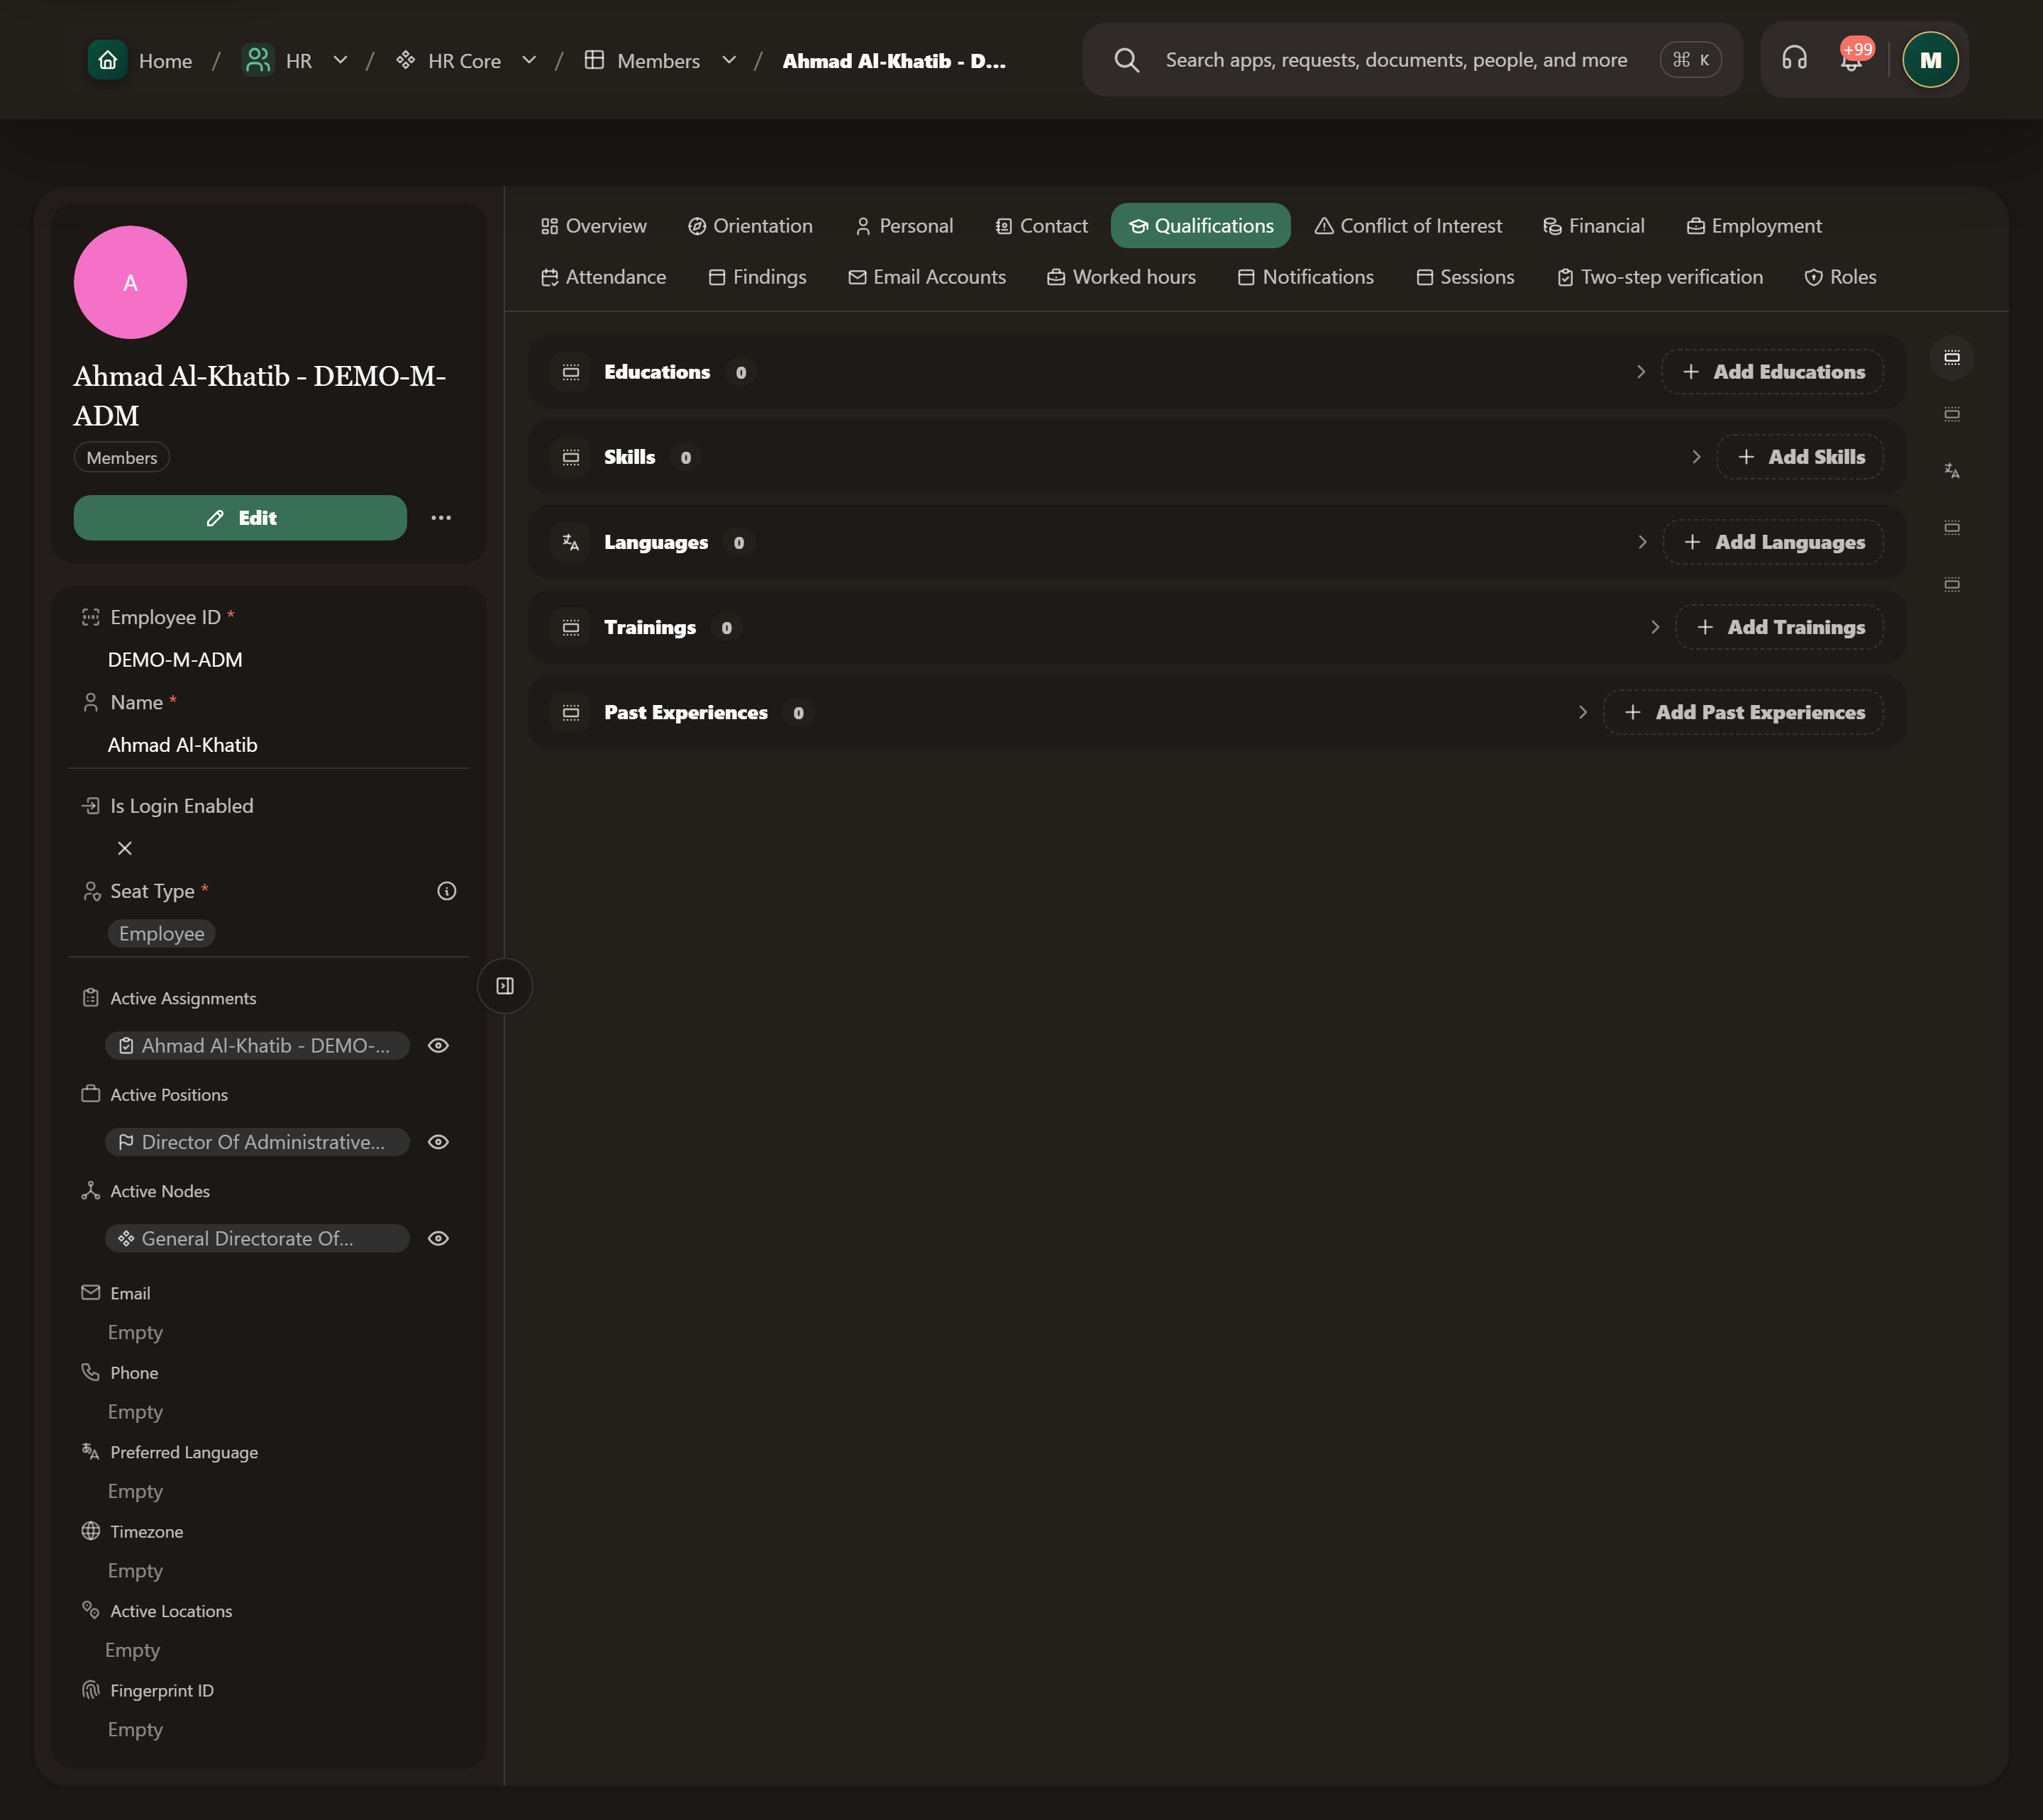
\includegraphics[width=0.95\linewidth]{figures/screens/ch03-member-tab5-en.png}
\caption{Demo employee record — Qualifications tab}
\label{fig:hr-member-tab5}
\end{figure}

\begin{figure}[H]
\centering
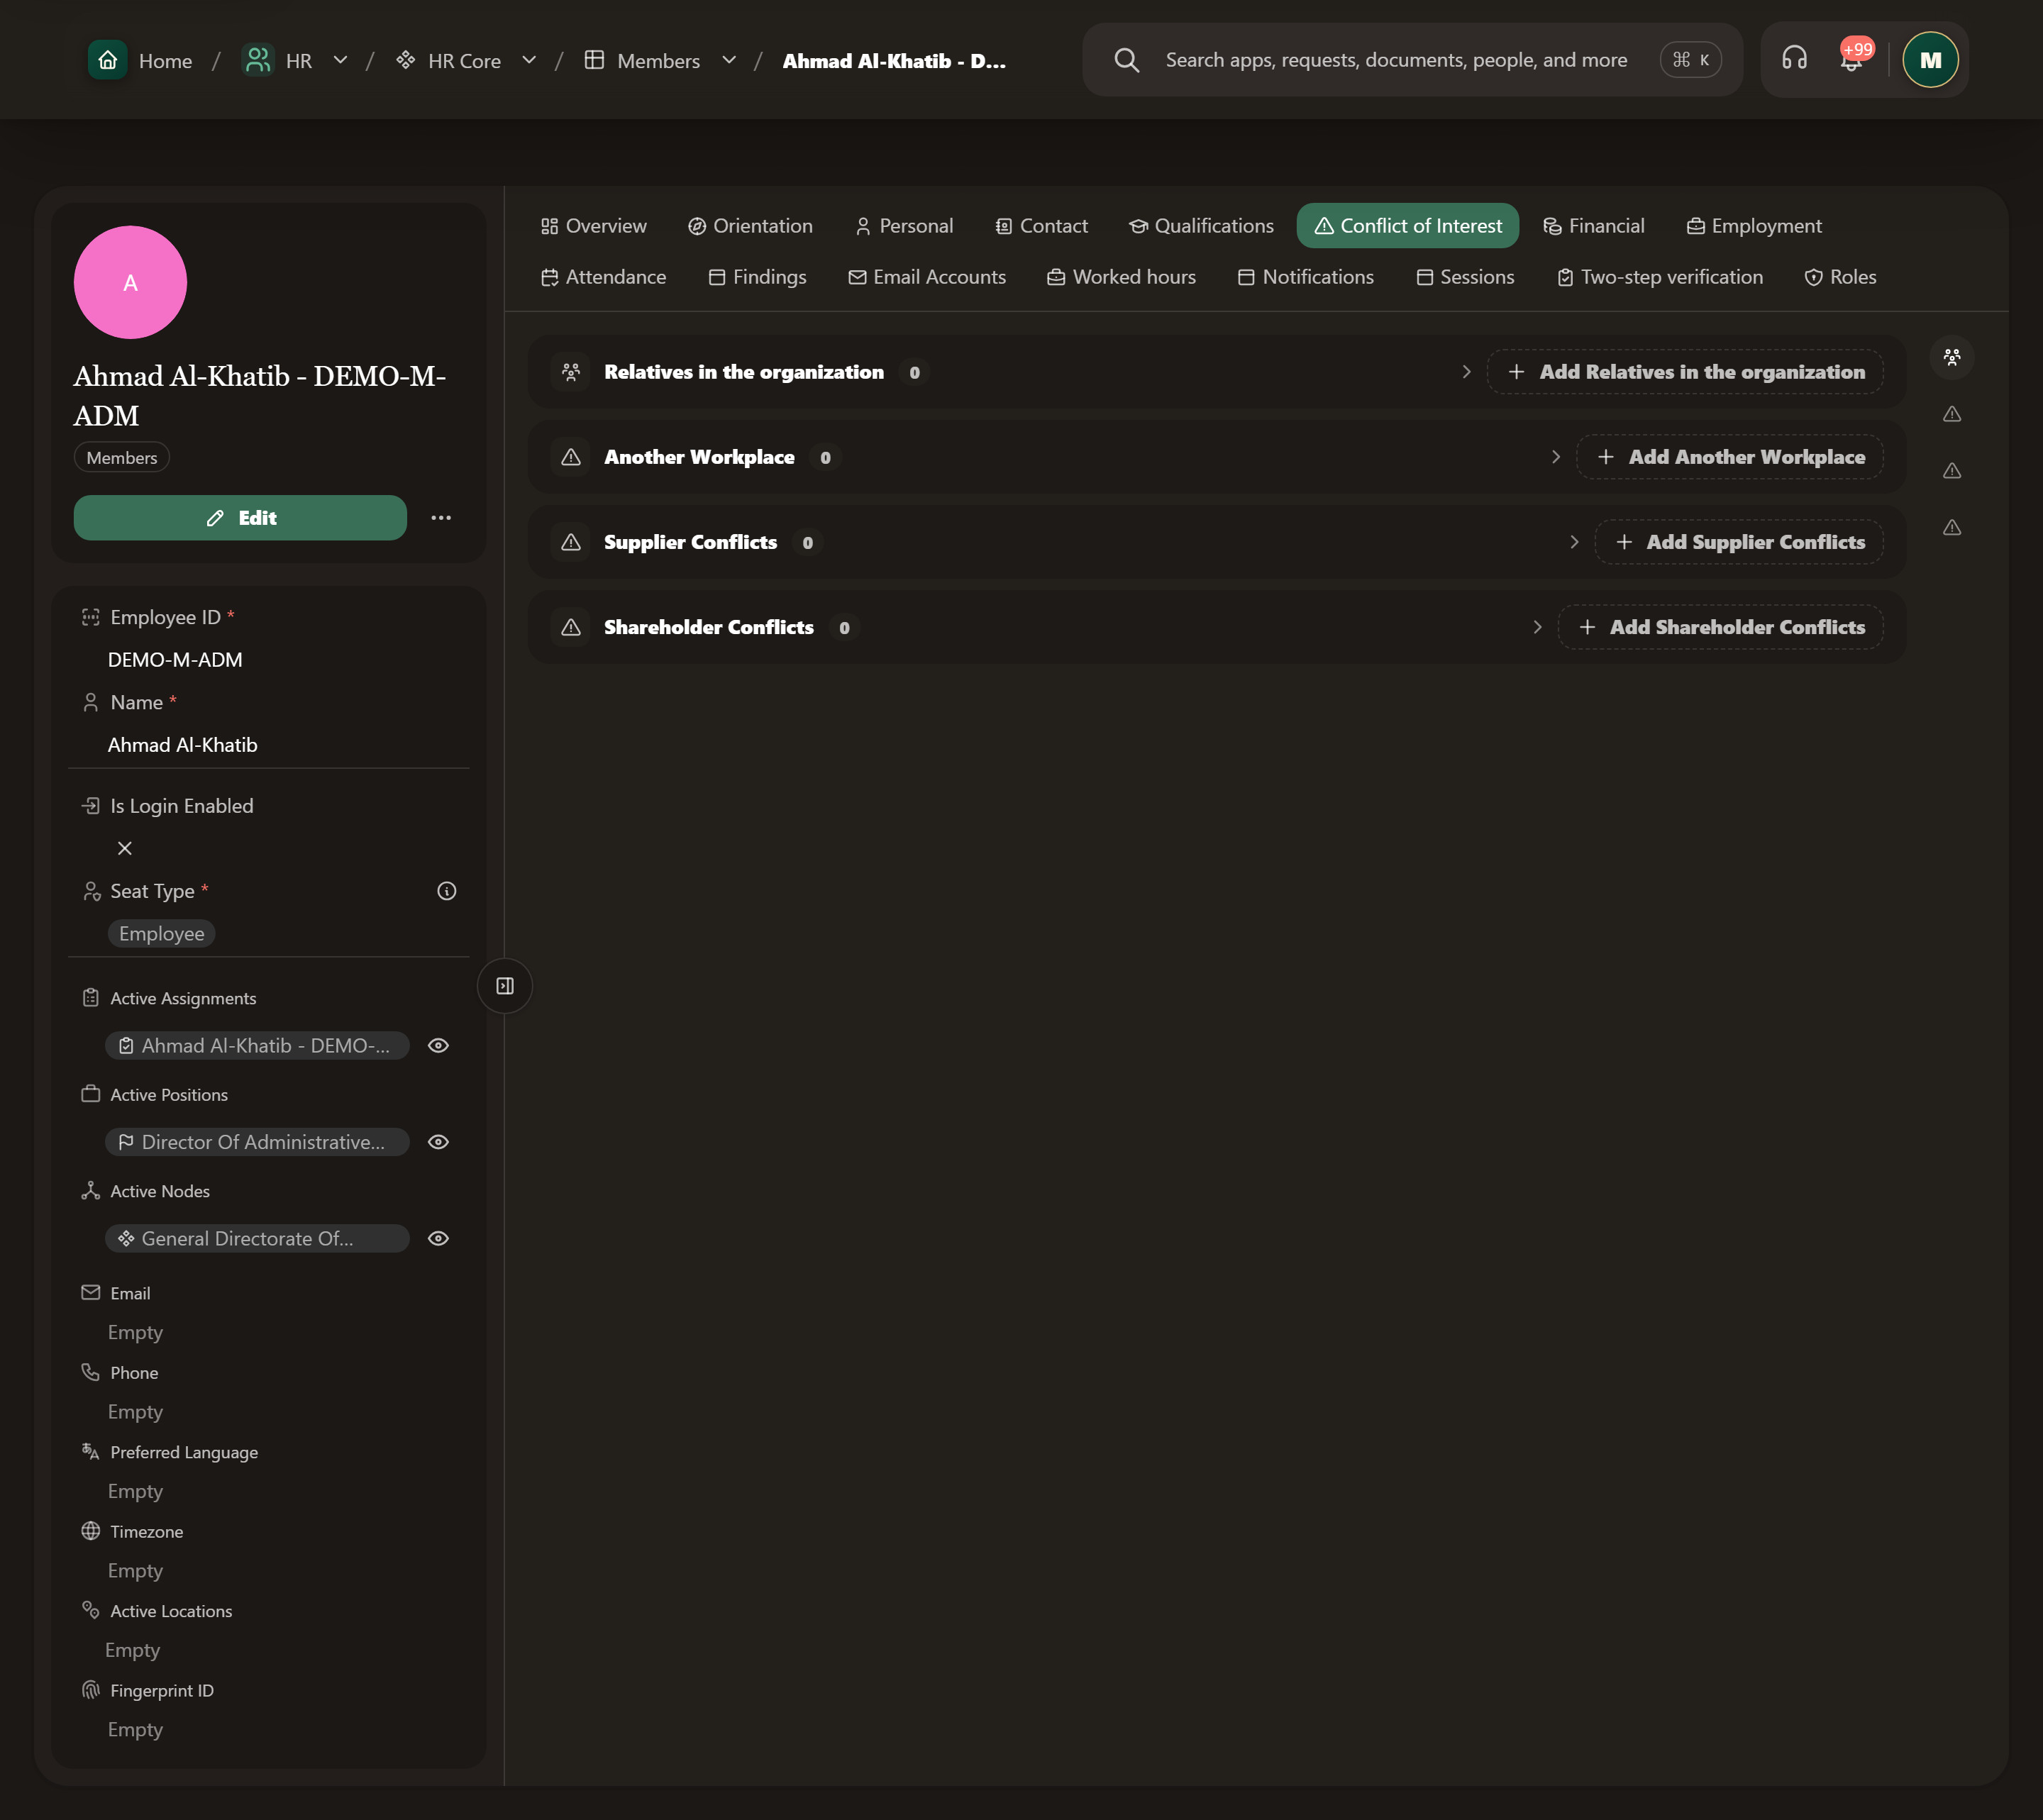
\includegraphics[width=0.95\linewidth]{figures/screens/ch03-member-tab6-en.png}
\caption{Demo employee record — Conflict of interest tab}
\label{fig:hr-member-tab6}
\end{figure}

\begin{figure}[H]
\centering
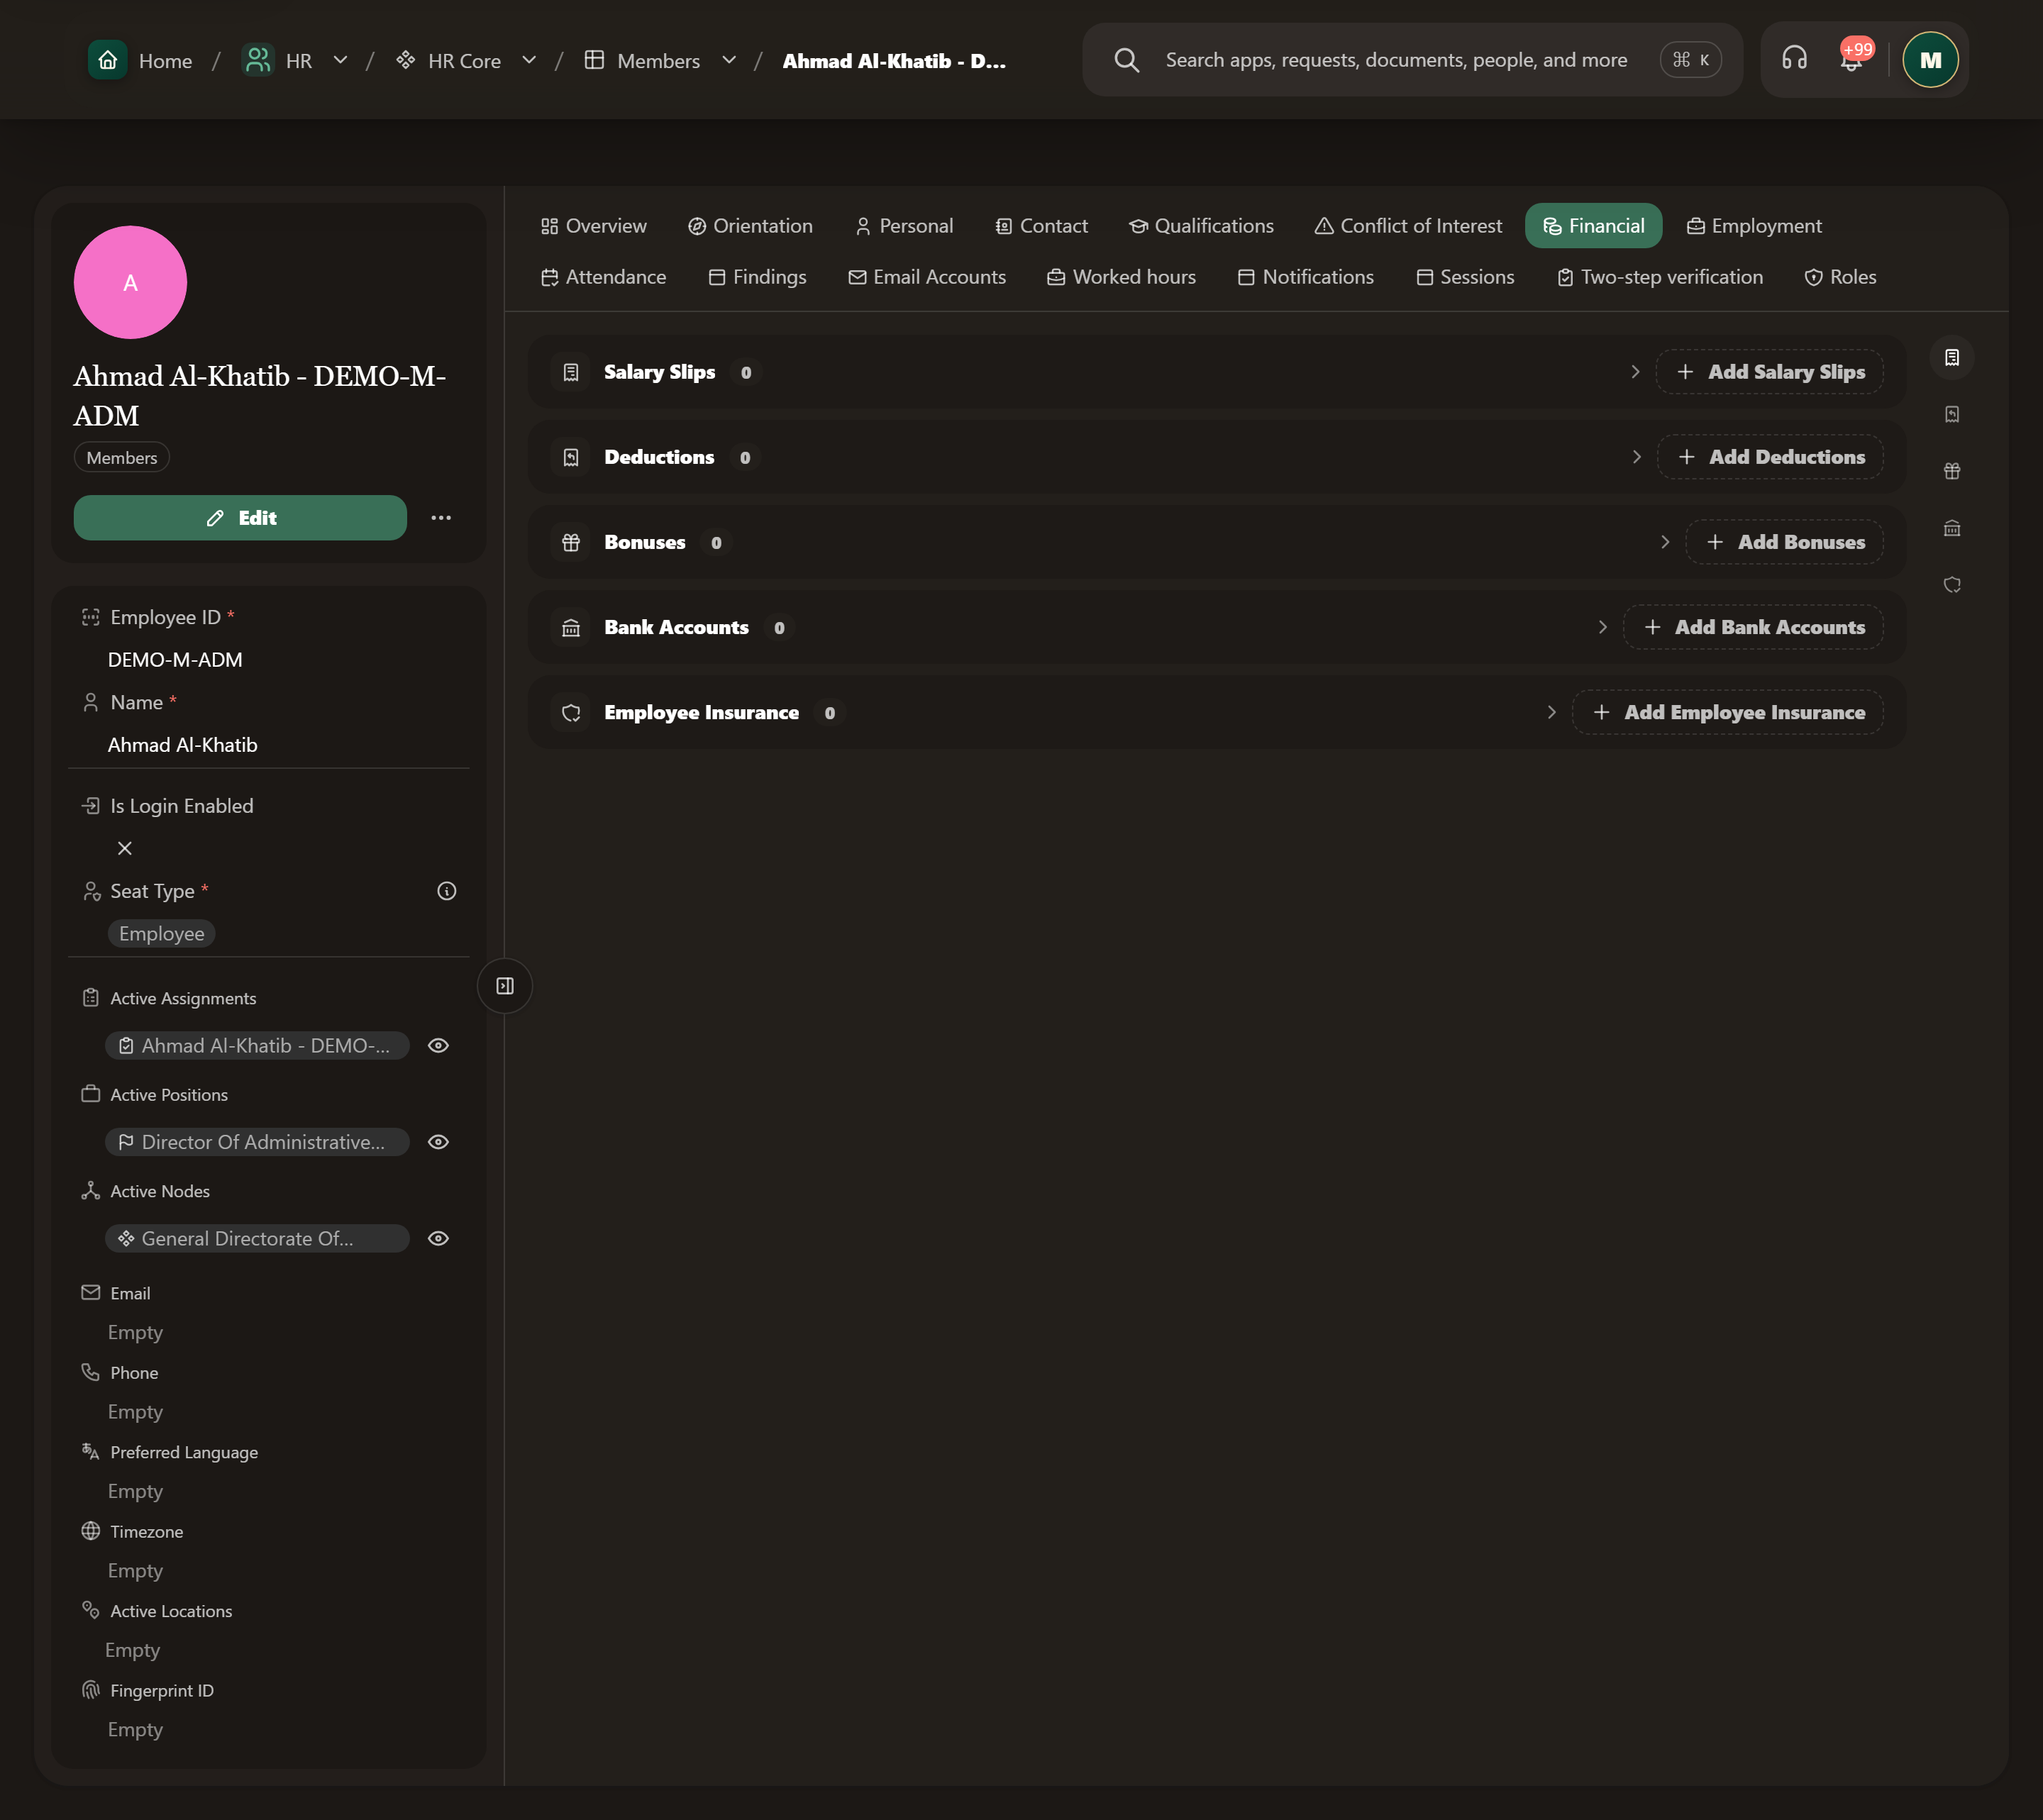
\includegraphics[width=0.95\linewidth]{figures/screens/ch03-member-tab7-en.png}
\caption{Demo employee record — Financial tab}
\label{fig:hr-member-tab7}
\end{figure}

\begin{figure}[H]
\centering
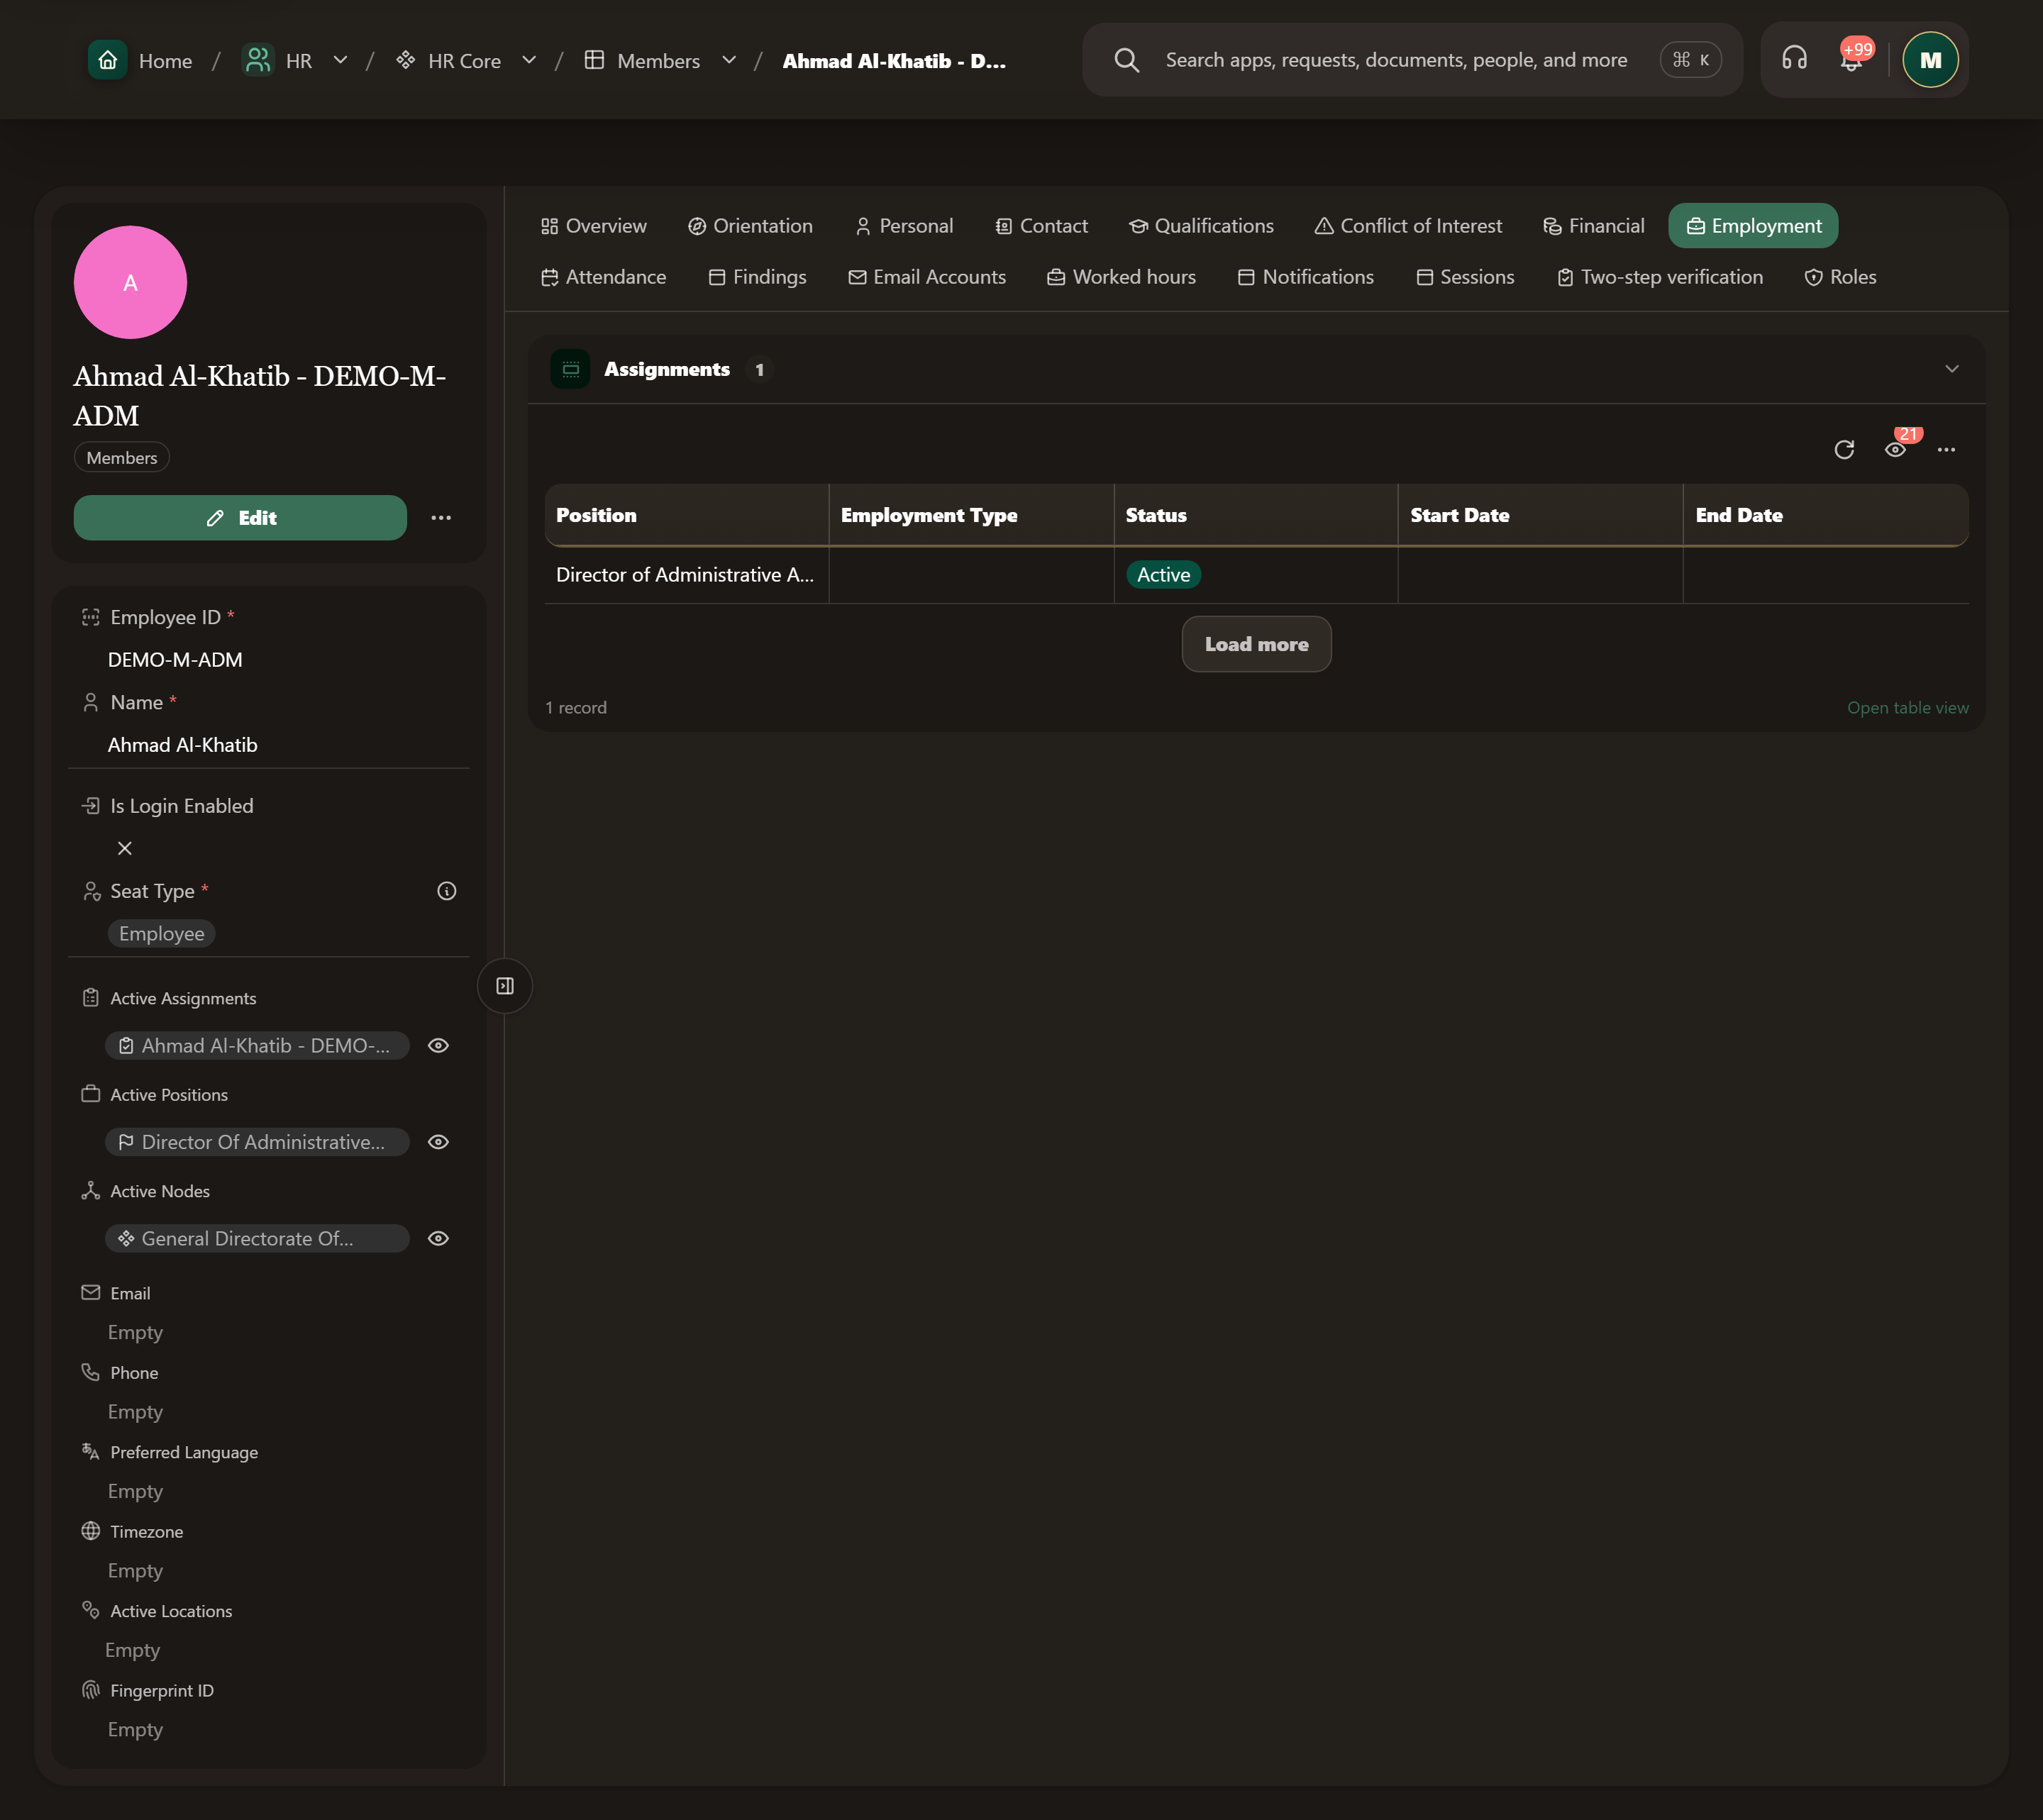
\includegraphics[width=0.95\linewidth]{figures/screens/ch03-member-tab8-en.png}
\caption{Demo employee record — Employment tab}
\label{fig:hr-member-tab8}
\end{figure}

\begin{figure}[H]
\centering
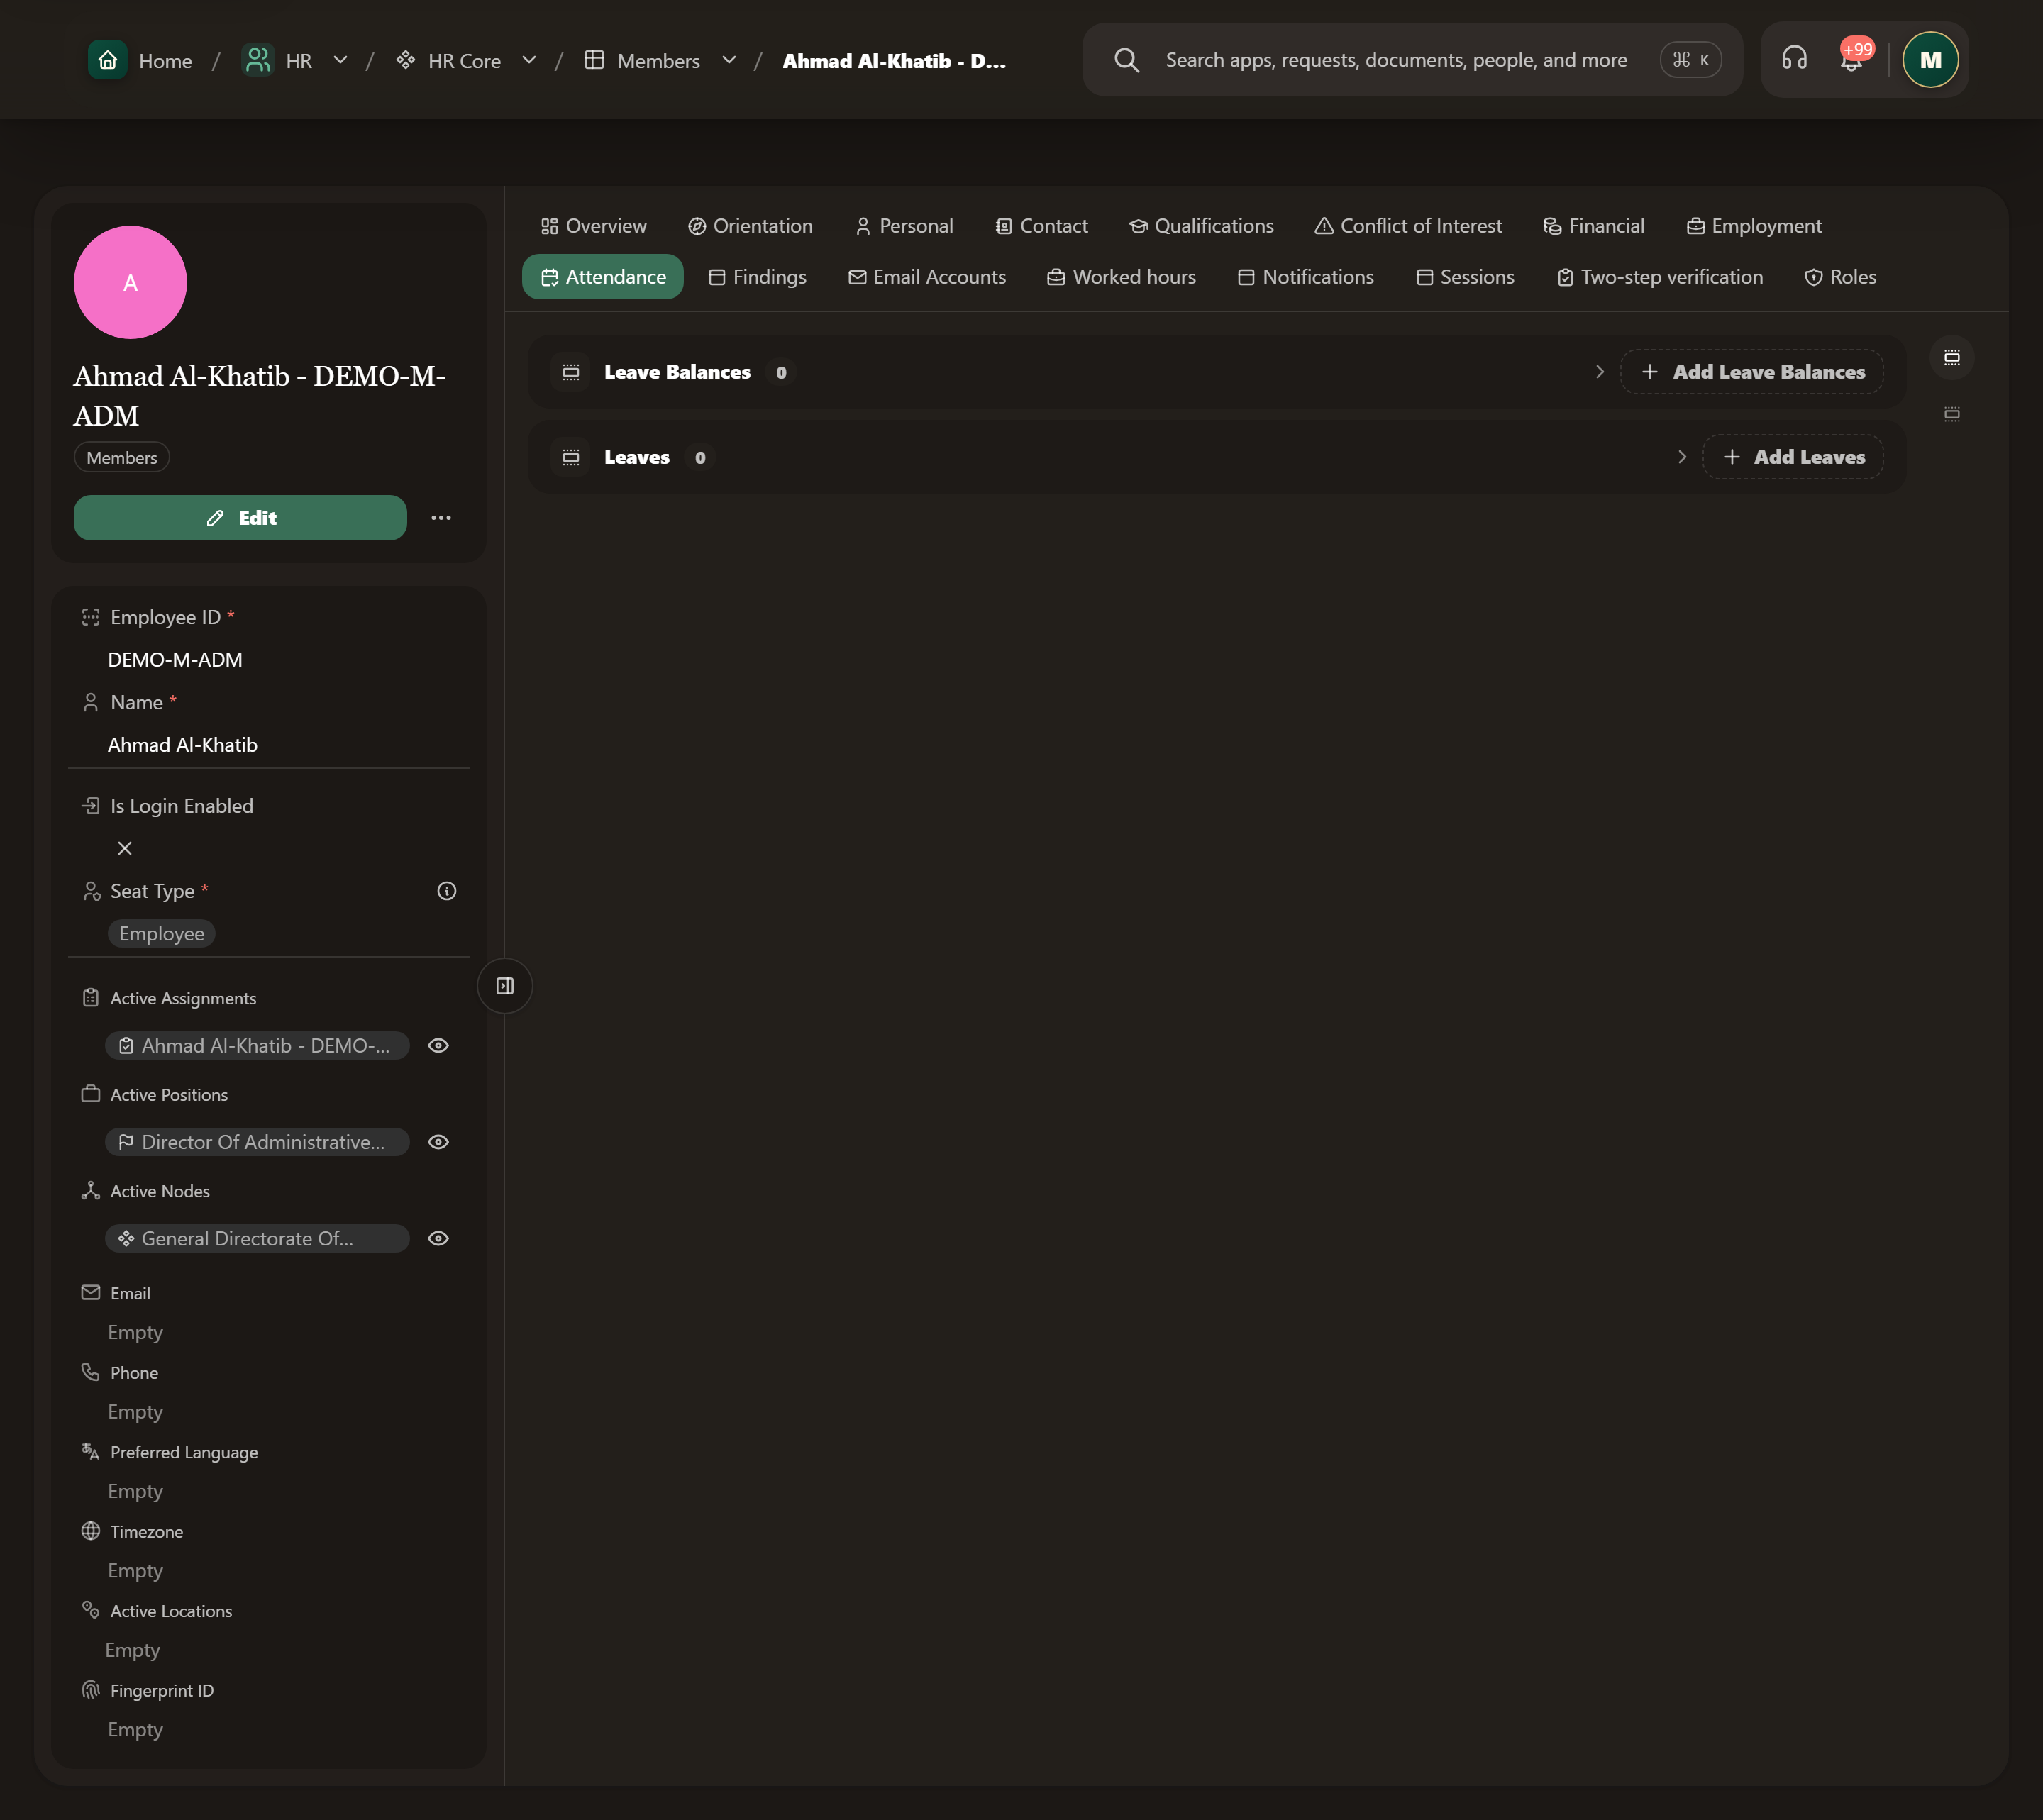
\includegraphics[width=0.95\linewidth]{figures/screens/ch03-member-tab9-en.png}
\caption{Demo employee record — Attendance tab}
\label{fig:hr-member-tab9}
\end{figure}



\begin{figure}[H]
\centering
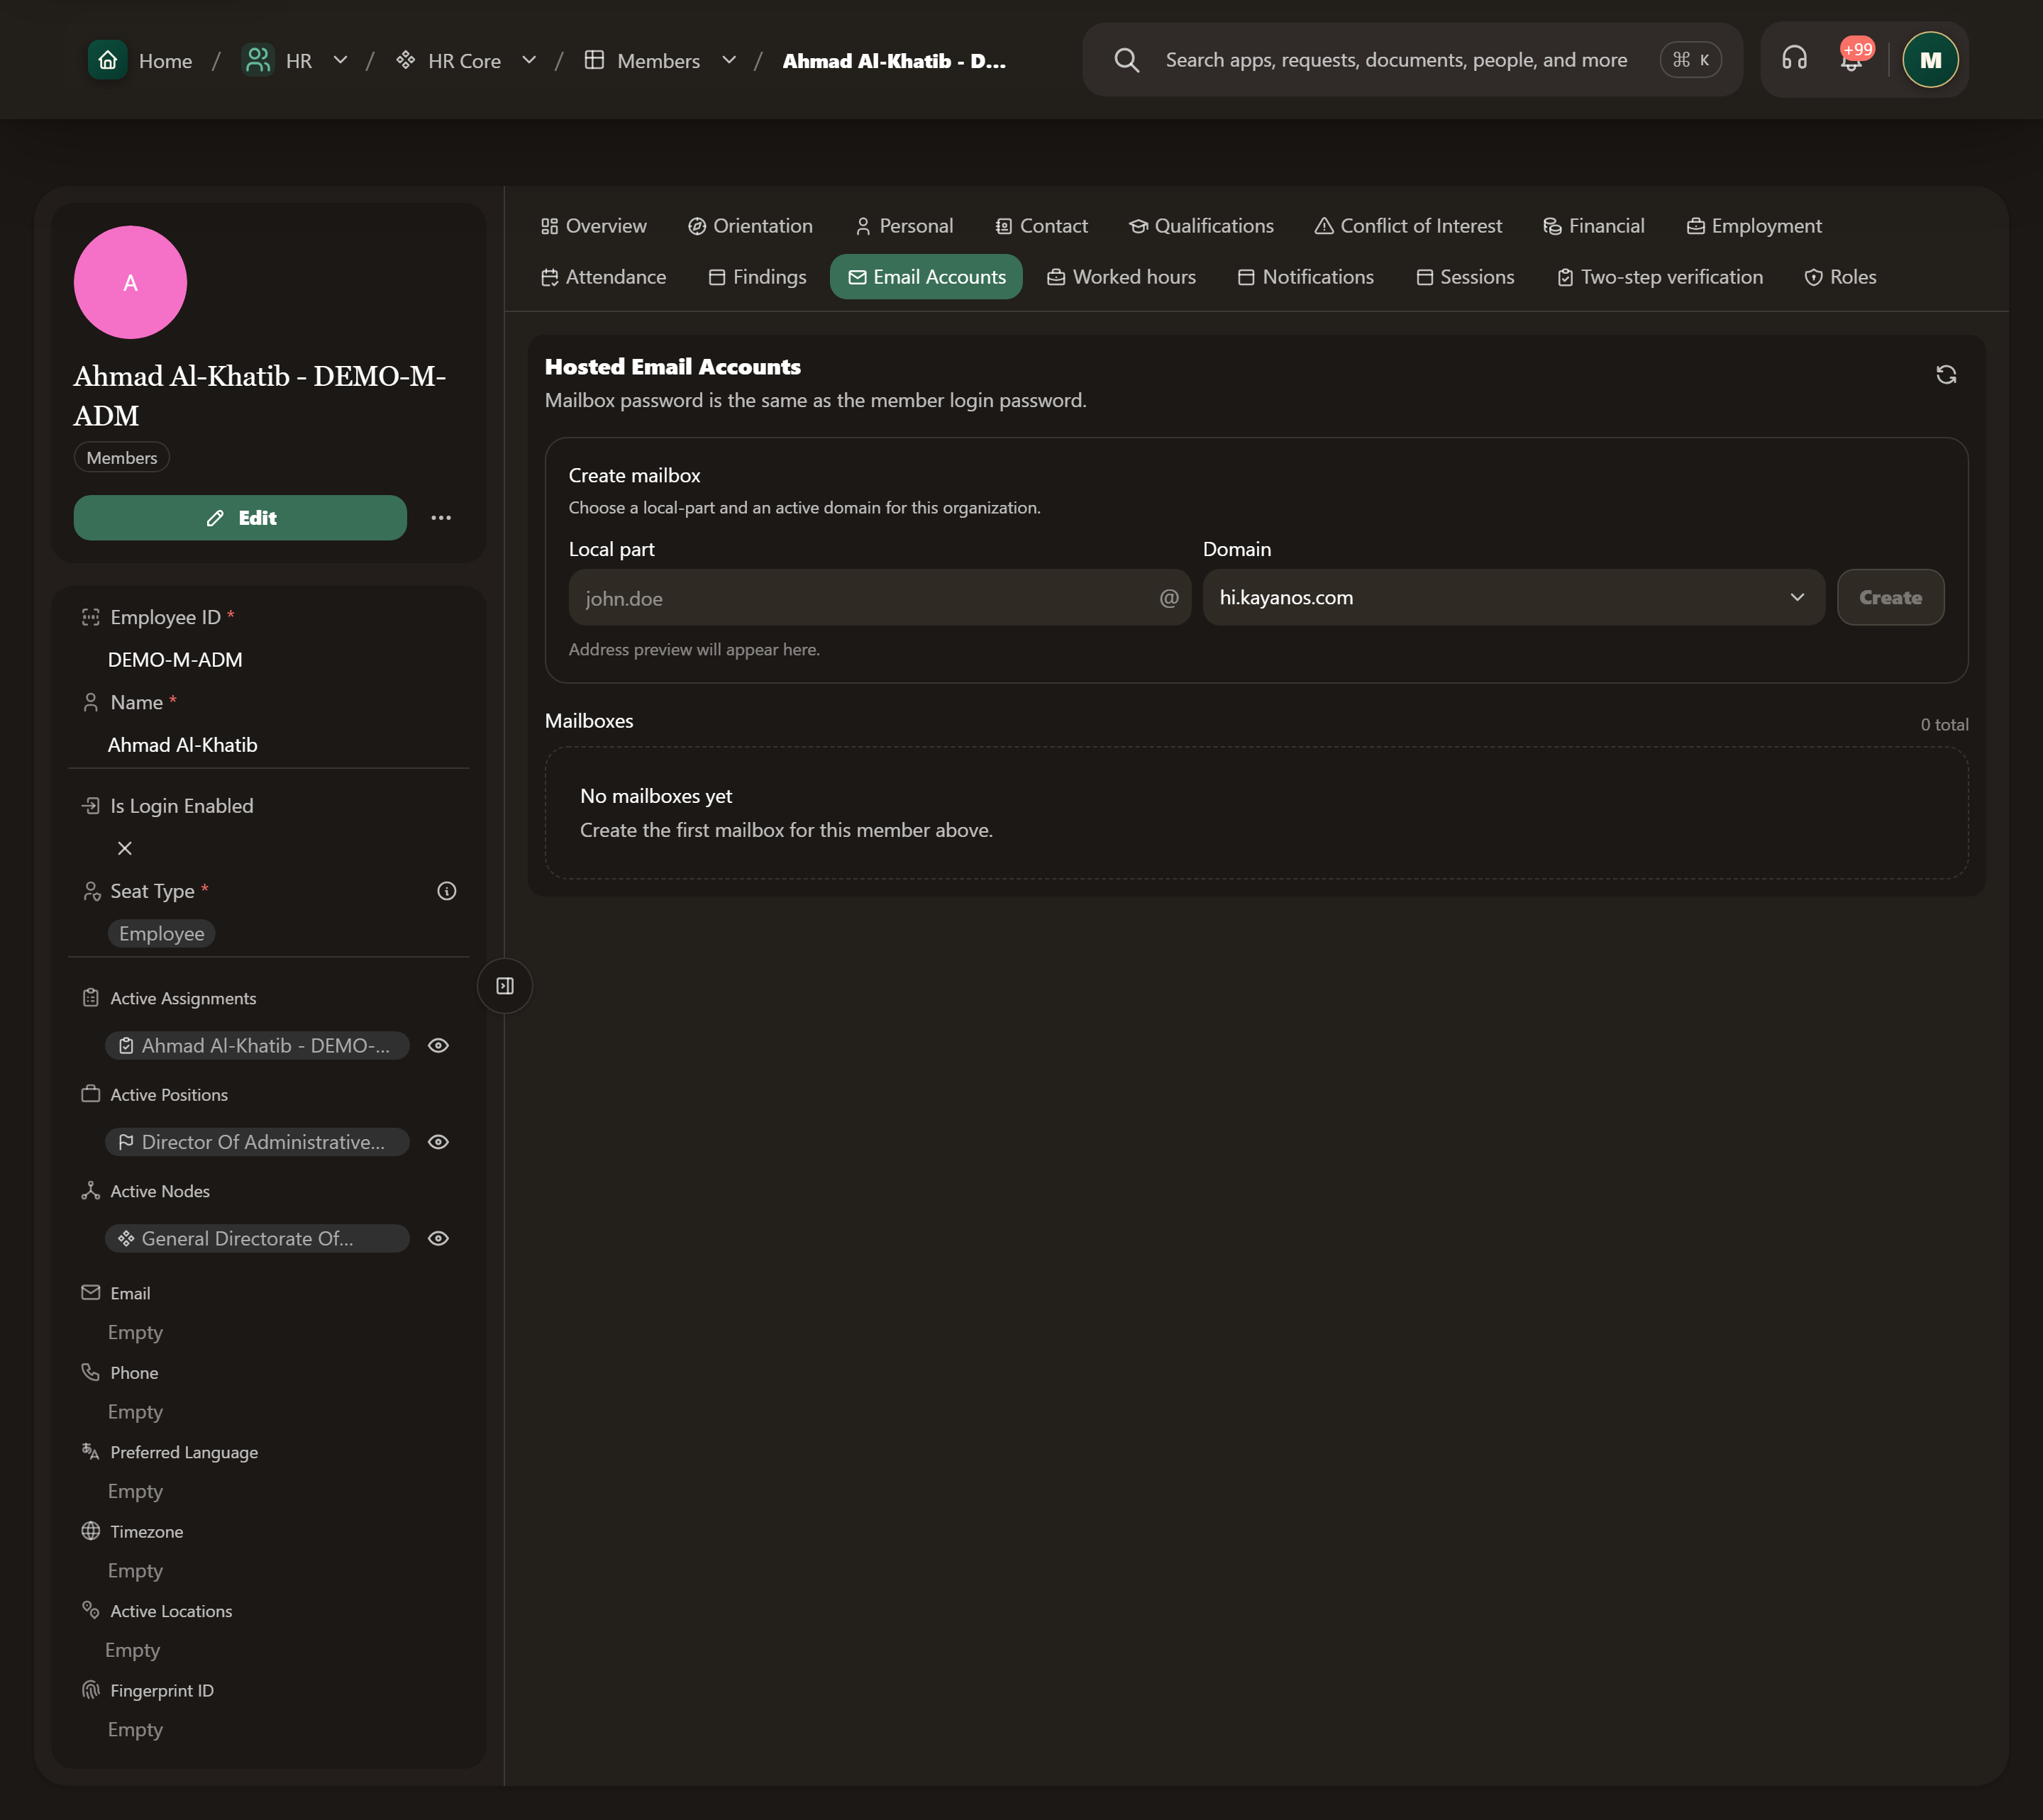
\includegraphics[width=0.95\linewidth]{figures/screens/ch03-member-tab11-en.png}
\caption{Demo employee record — Email accounts tab}
\label{fig:hr-member-tab11}
\end{figure}

\begin{figure}[H]
\centering
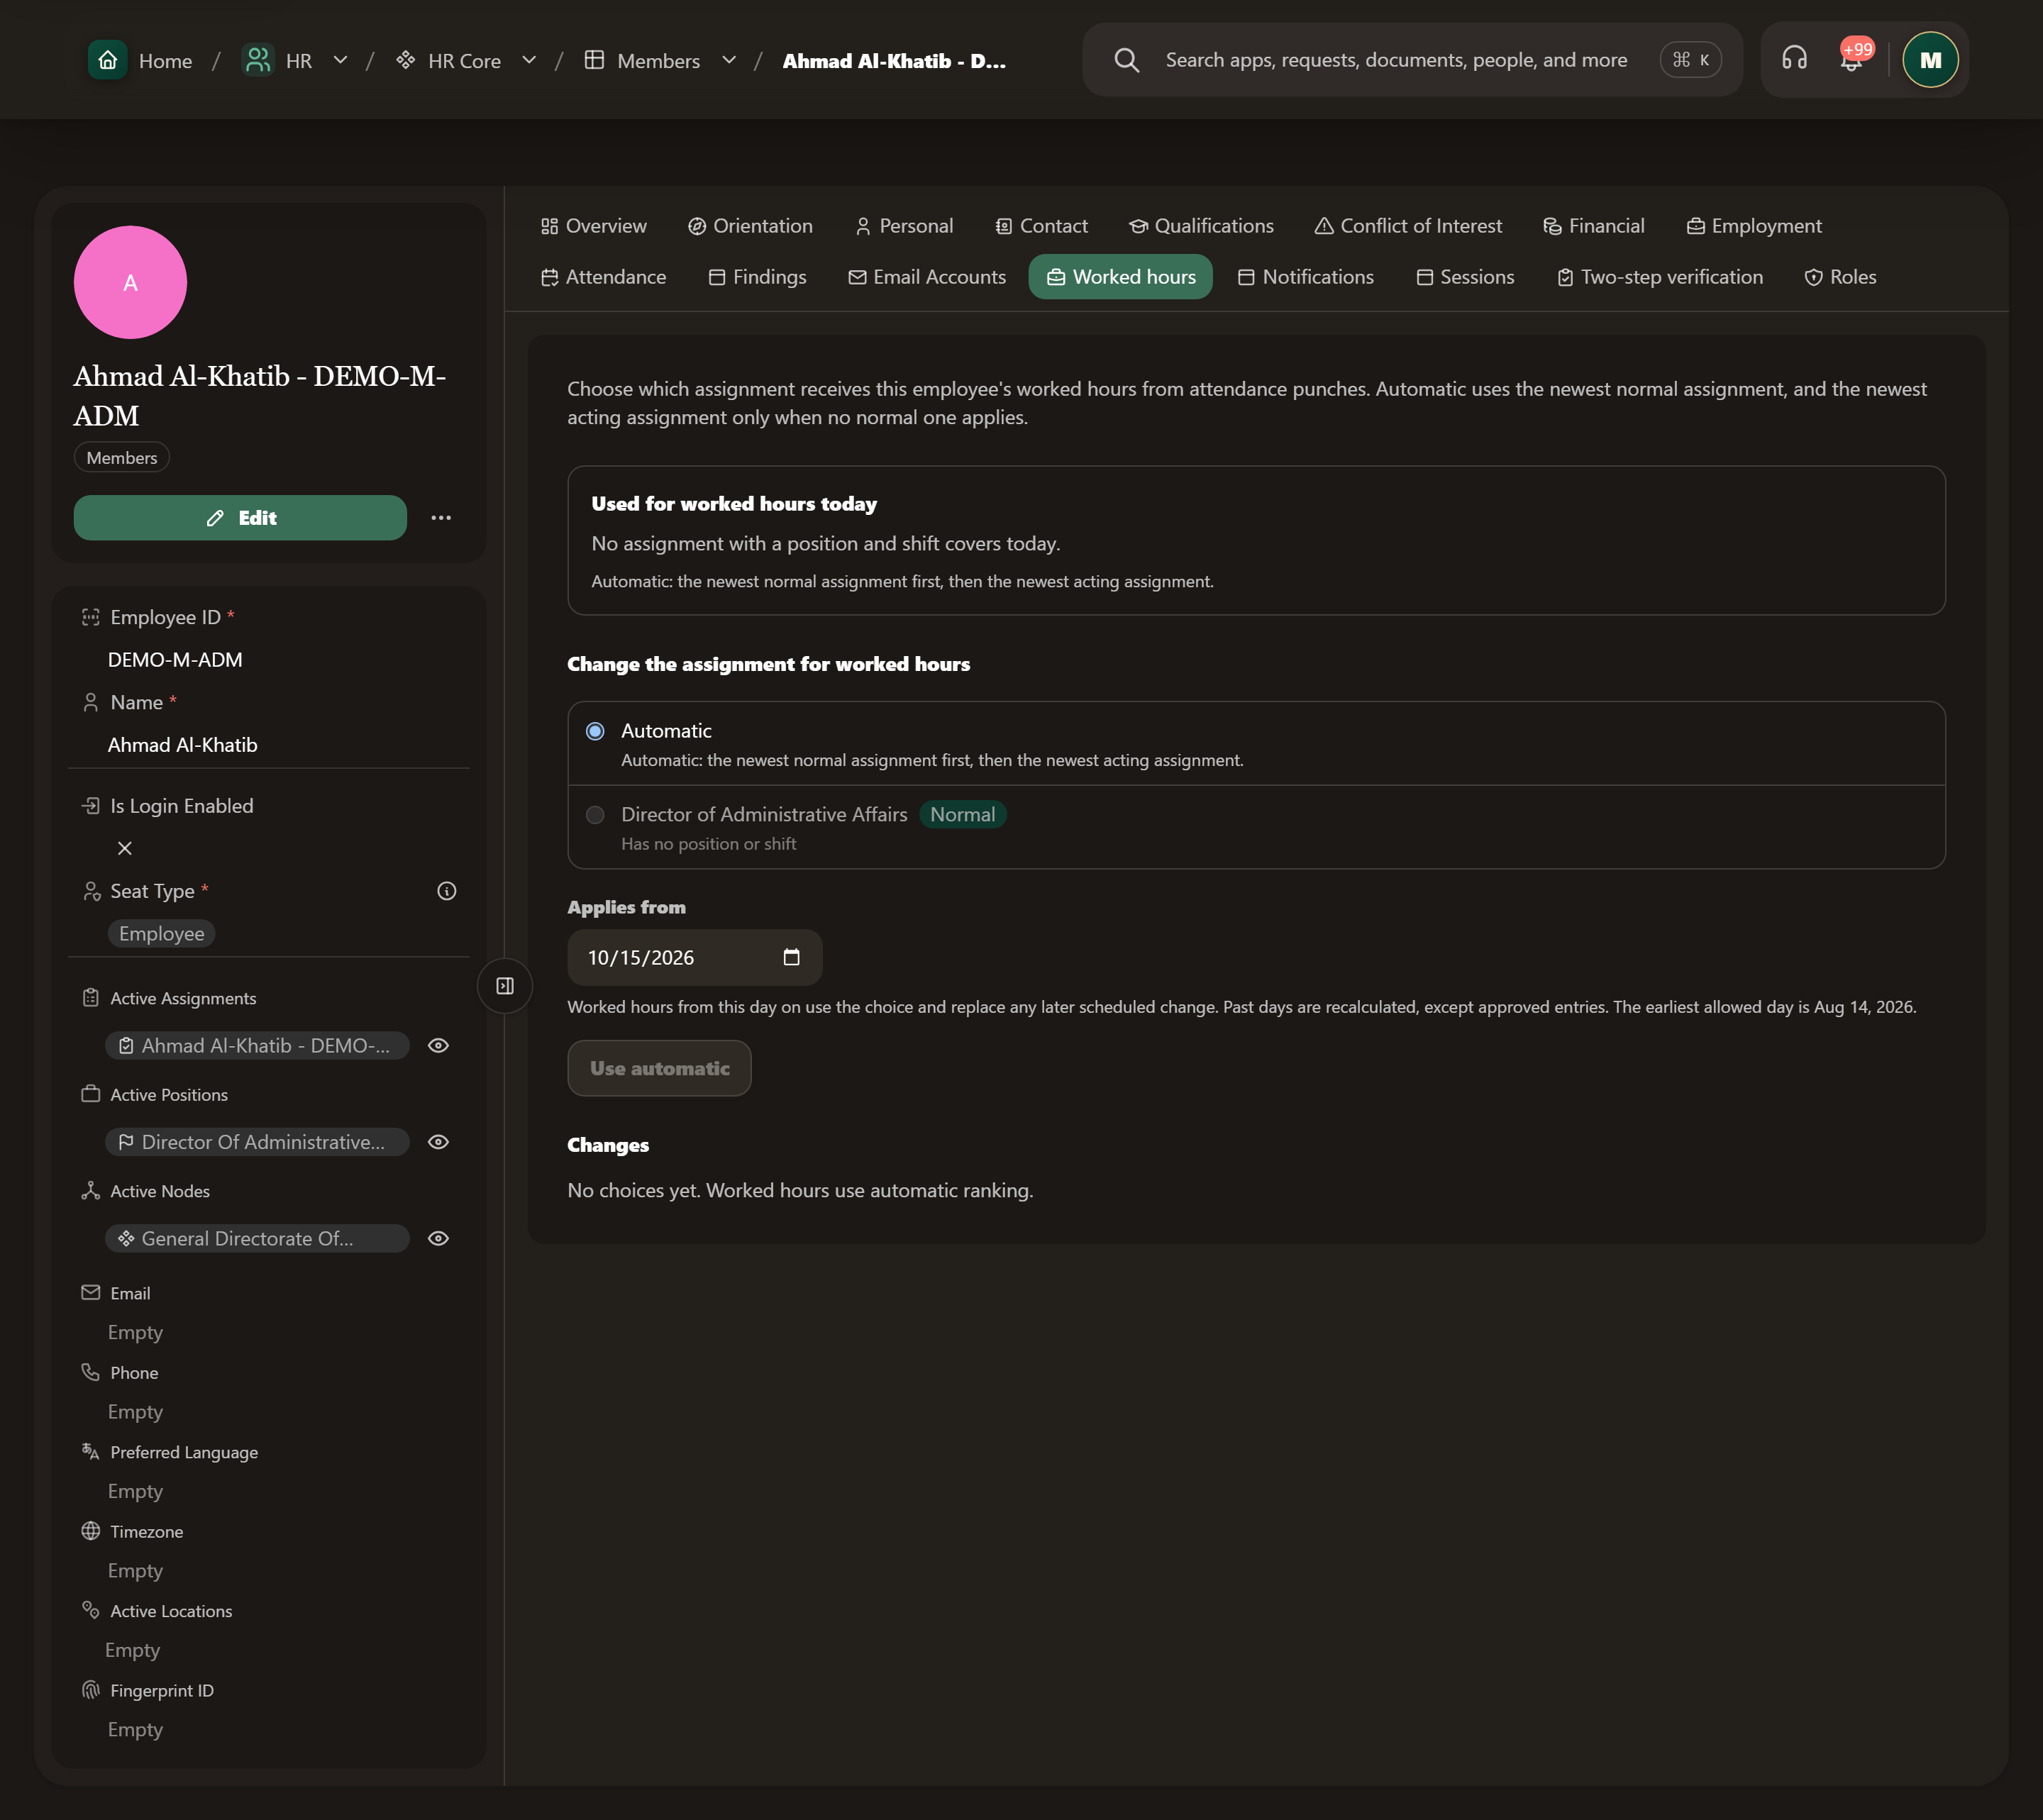
\includegraphics[width=0.95\linewidth]{figures/screens/ch03-member-tab12-en.png}
\caption{Demo employee record — Worked hours tab}
\label{fig:hr-member-tab12}
\end{figure}

\begin{figure}[H]
\centering

\includegraphics[width=0.95\linewidth]{figures/screens/ch03-member-tab13-en.png}
\caption{Demo employee record — Notifications tab}
\label{fig:hr-member-tab13}
\end{figure}

\begin{figure}[H]
\centering
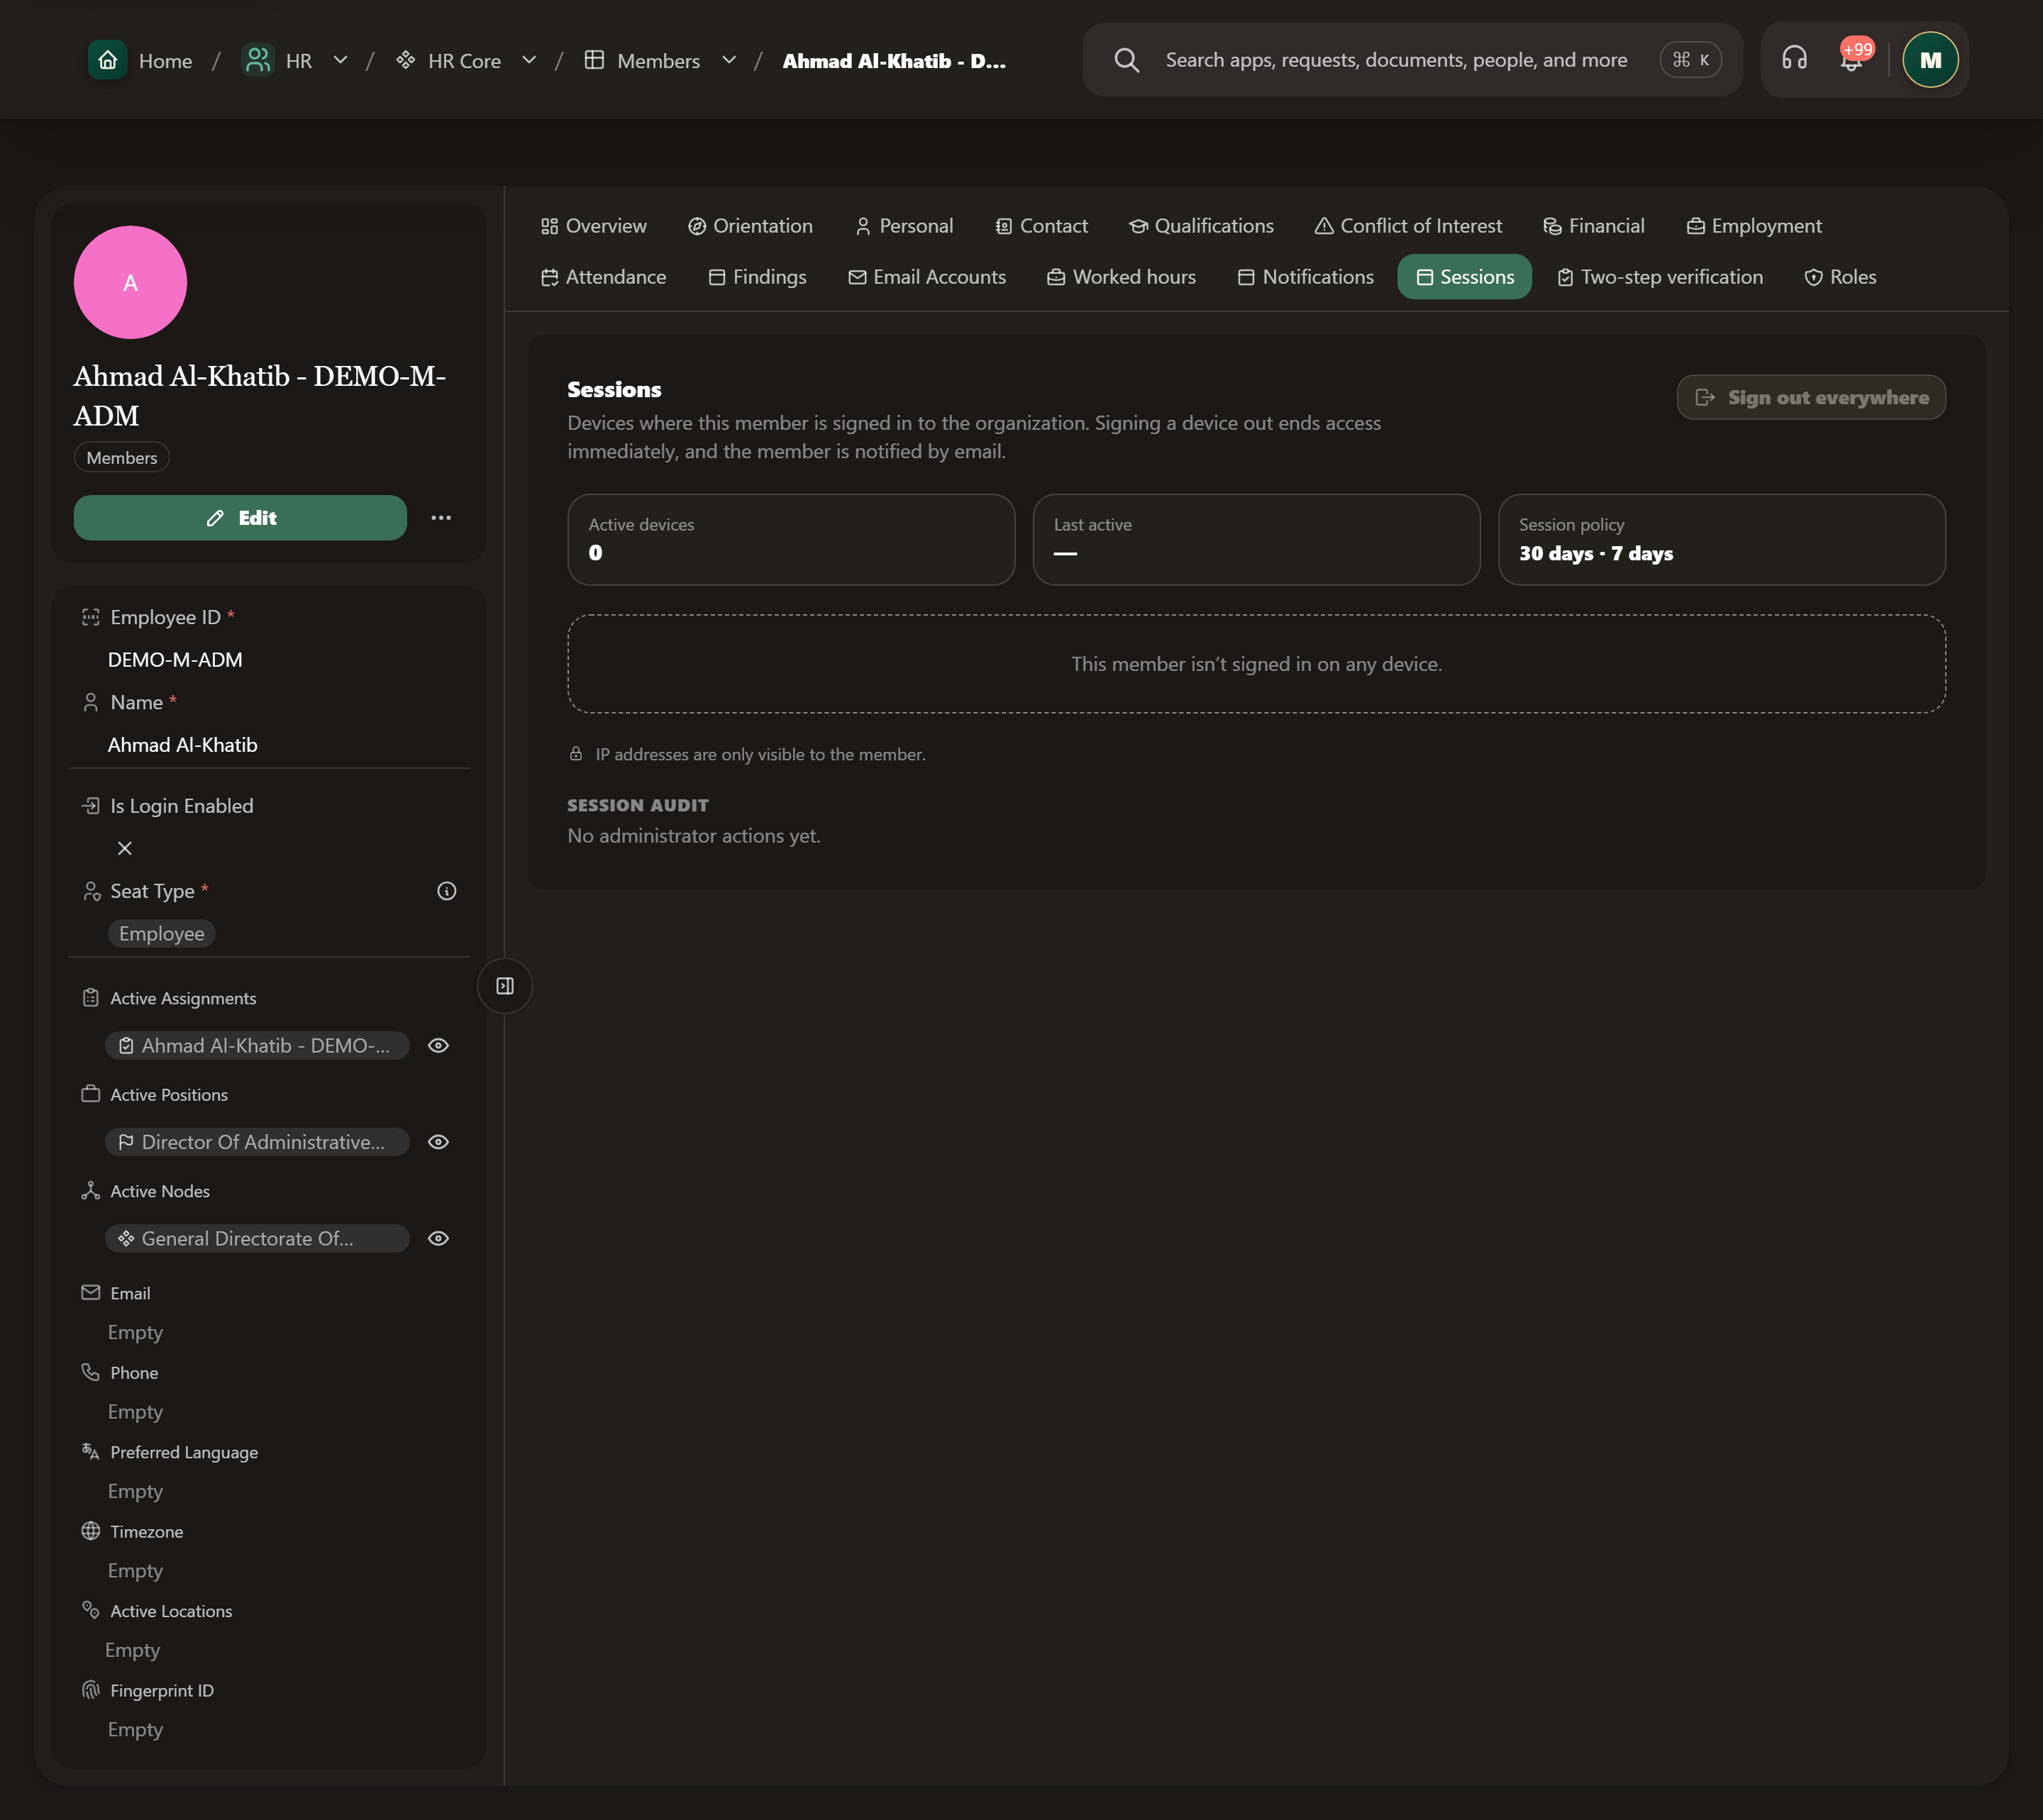
\includegraphics[width=0.95\linewidth]{figures/screens/ch03-member-tab14-en.png}
\caption{Demo employee record — Sessions tab}
\label{fig:hr-member-tab14}
\end{figure}

\begin{figure}[H]
\centering
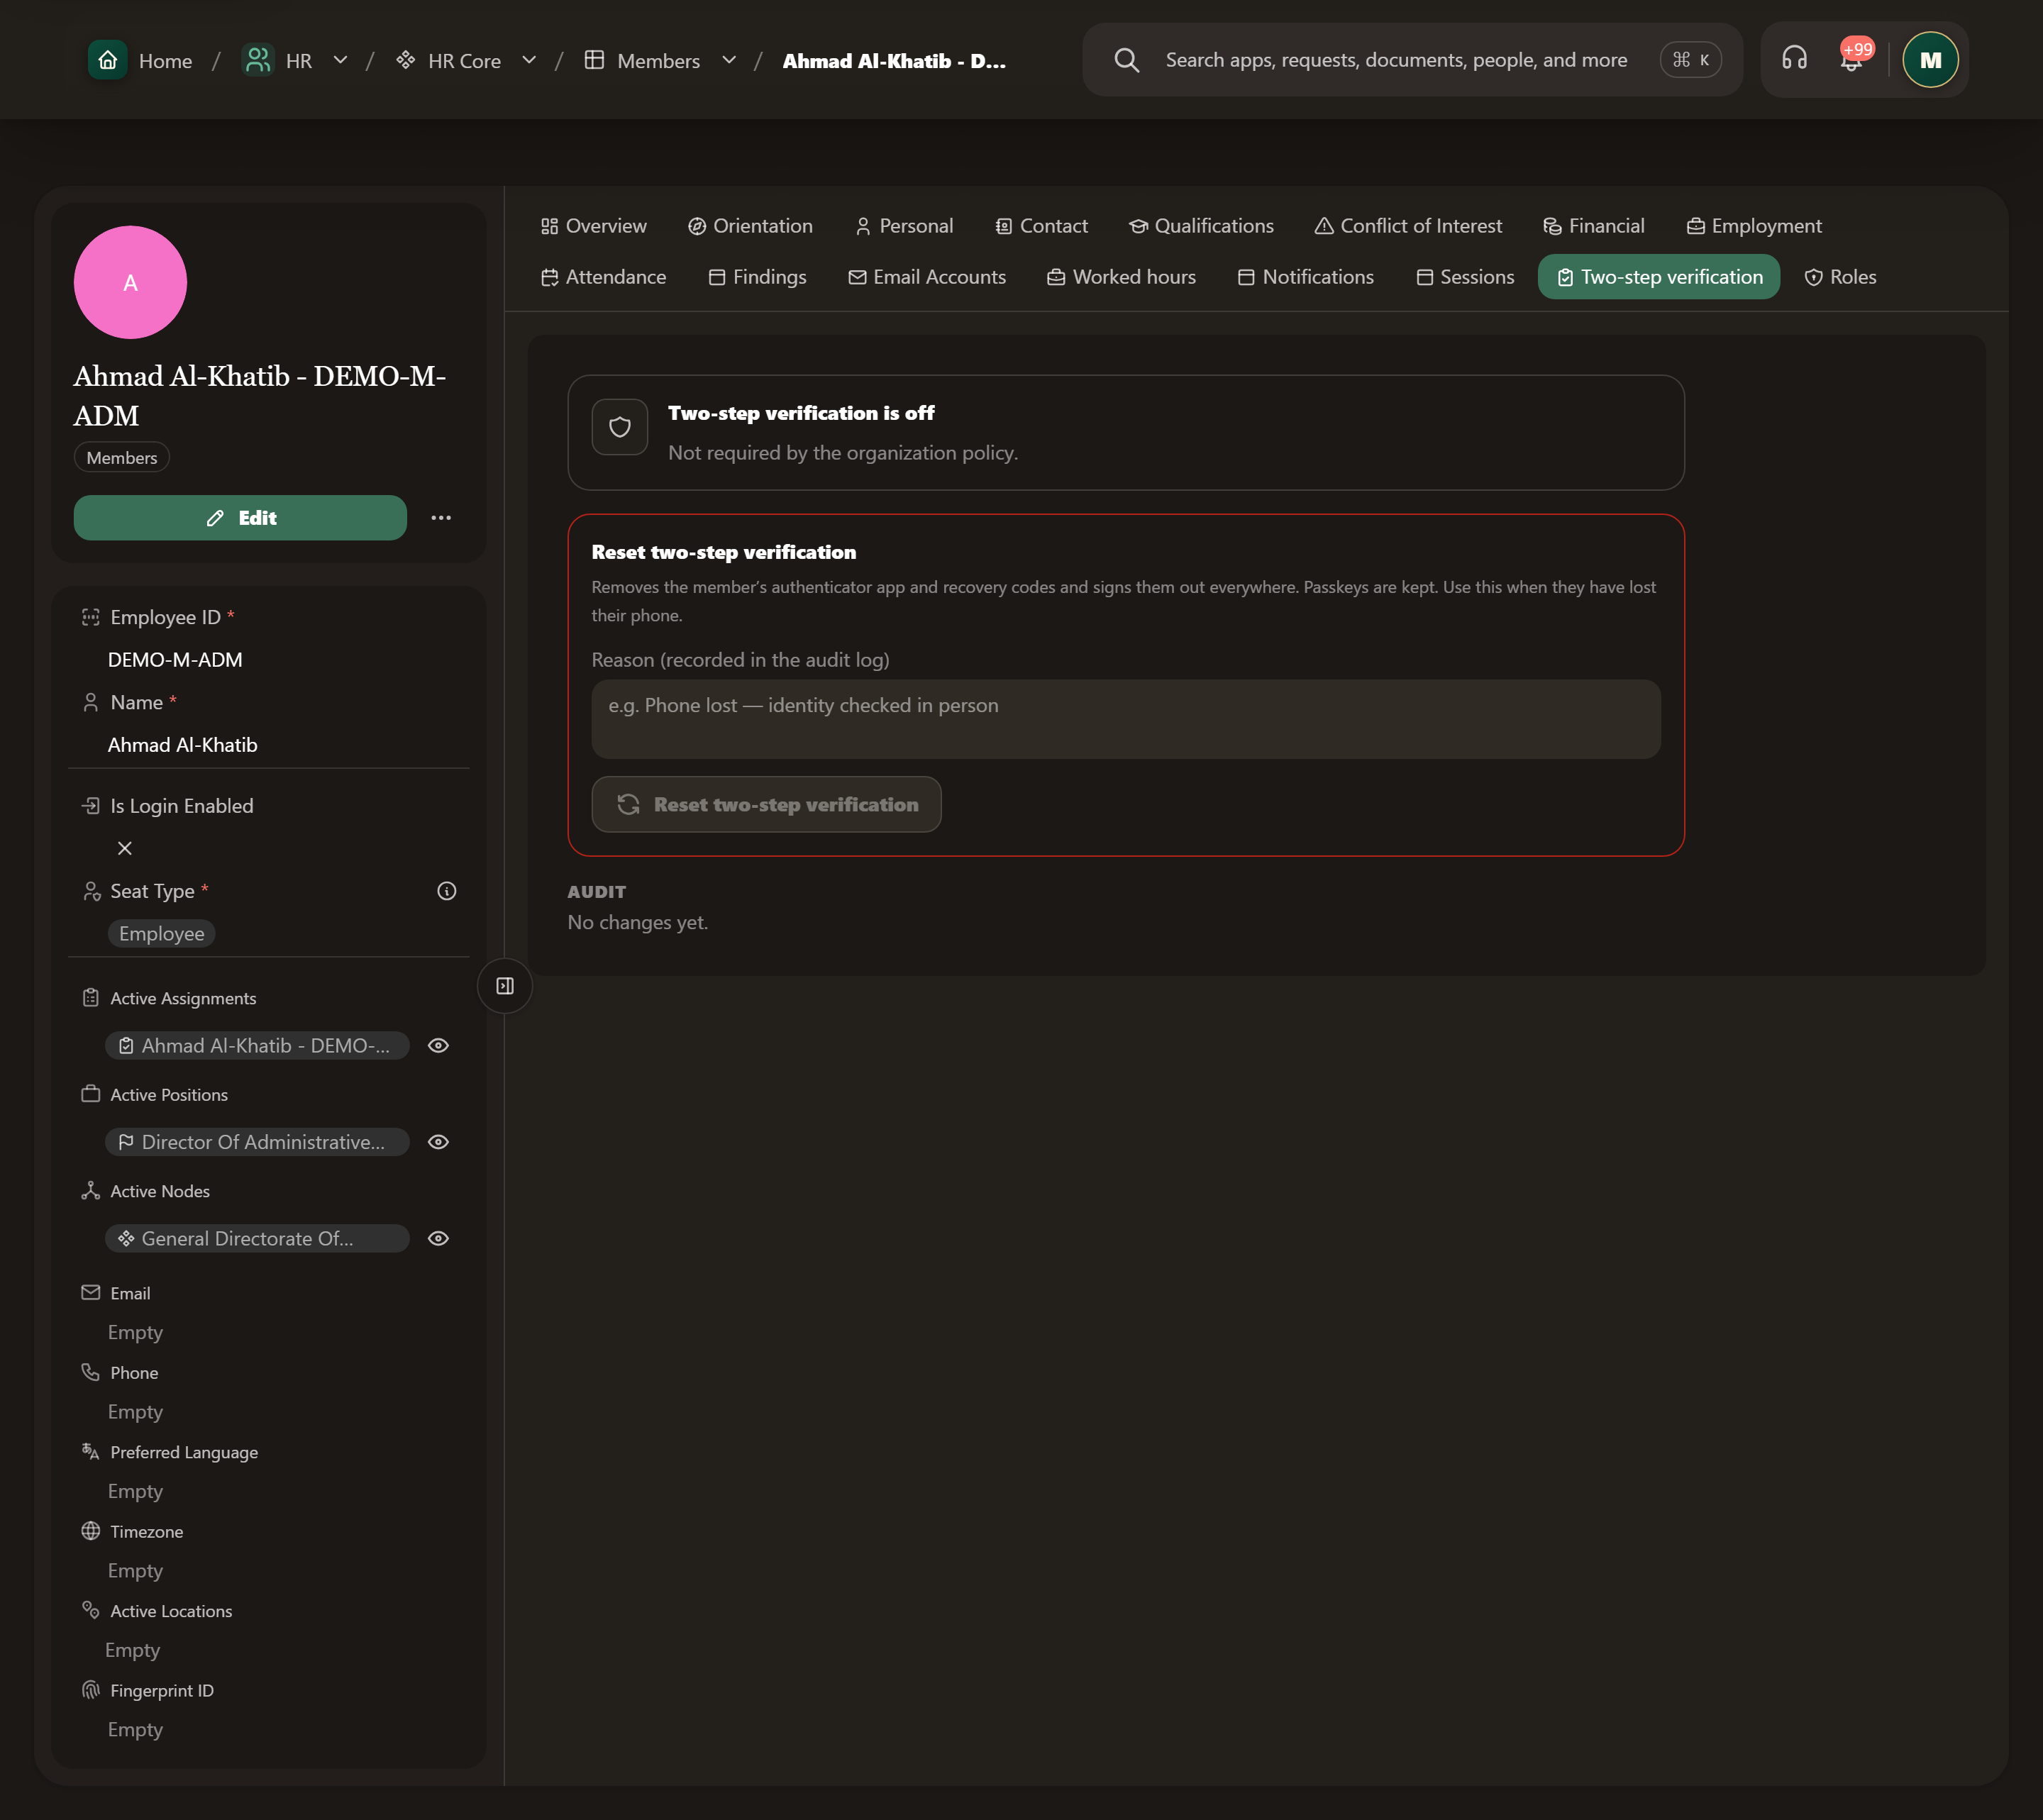
\includegraphics[width=0.95\linewidth]{figures/screens/ch03-member-tab15-en.png}
\caption{Demo employee record — Two-step verification tab}
\label{fig:hr-member-tab15}
\end{figure}

\begin{figure}[H]
\centering
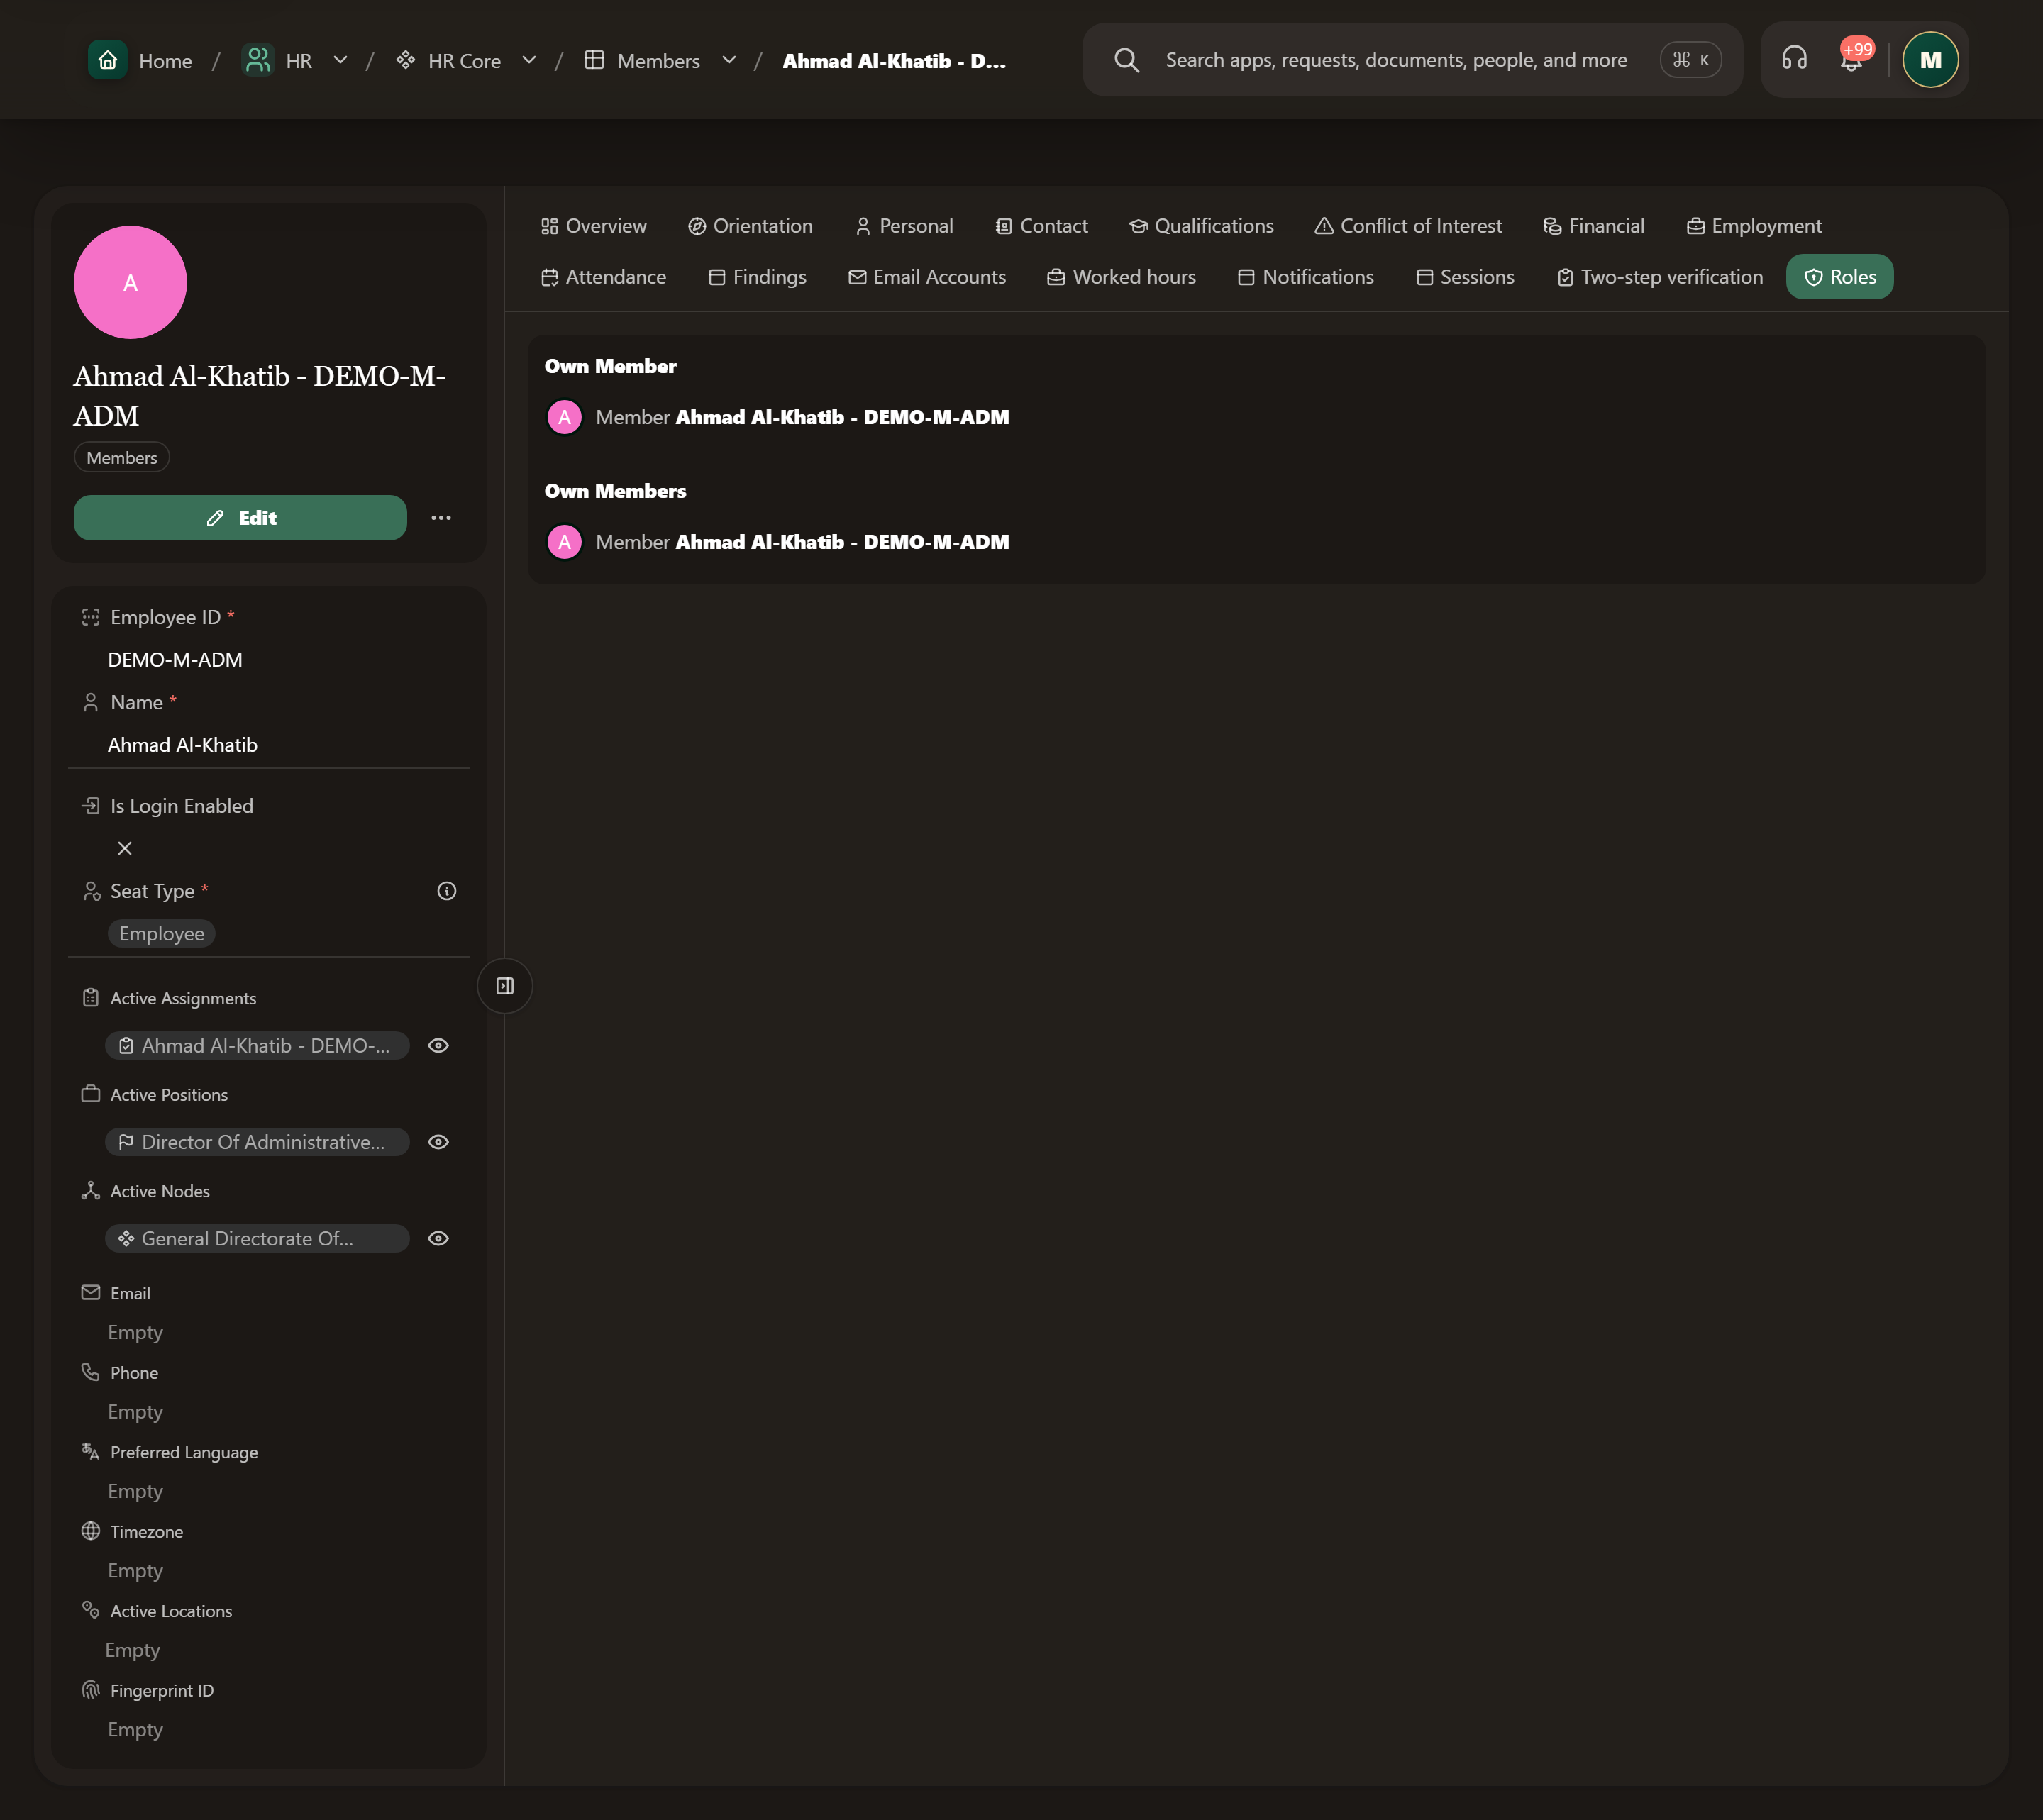
\includegraphics[width=0.95\linewidth]{figures/screens/ch03-member-tab16-en.png}
\caption{Demo employee record — Roles tab}
\label{fig:hr-member-tab16}
\end{figure}

\clearpage
\section{Positions}
\label{sec:hr-feature-positions}

A position is a job such as HR Manager. It sets the reporting line, unit, location and grade; an assignment sets who holds it.

\textbf{When is it useful?} Define the job once, then track who holds it or whether it is vacant. \textbf{Open:} HR / Workforce / Positions.

\begin{figure}[H]
\centering
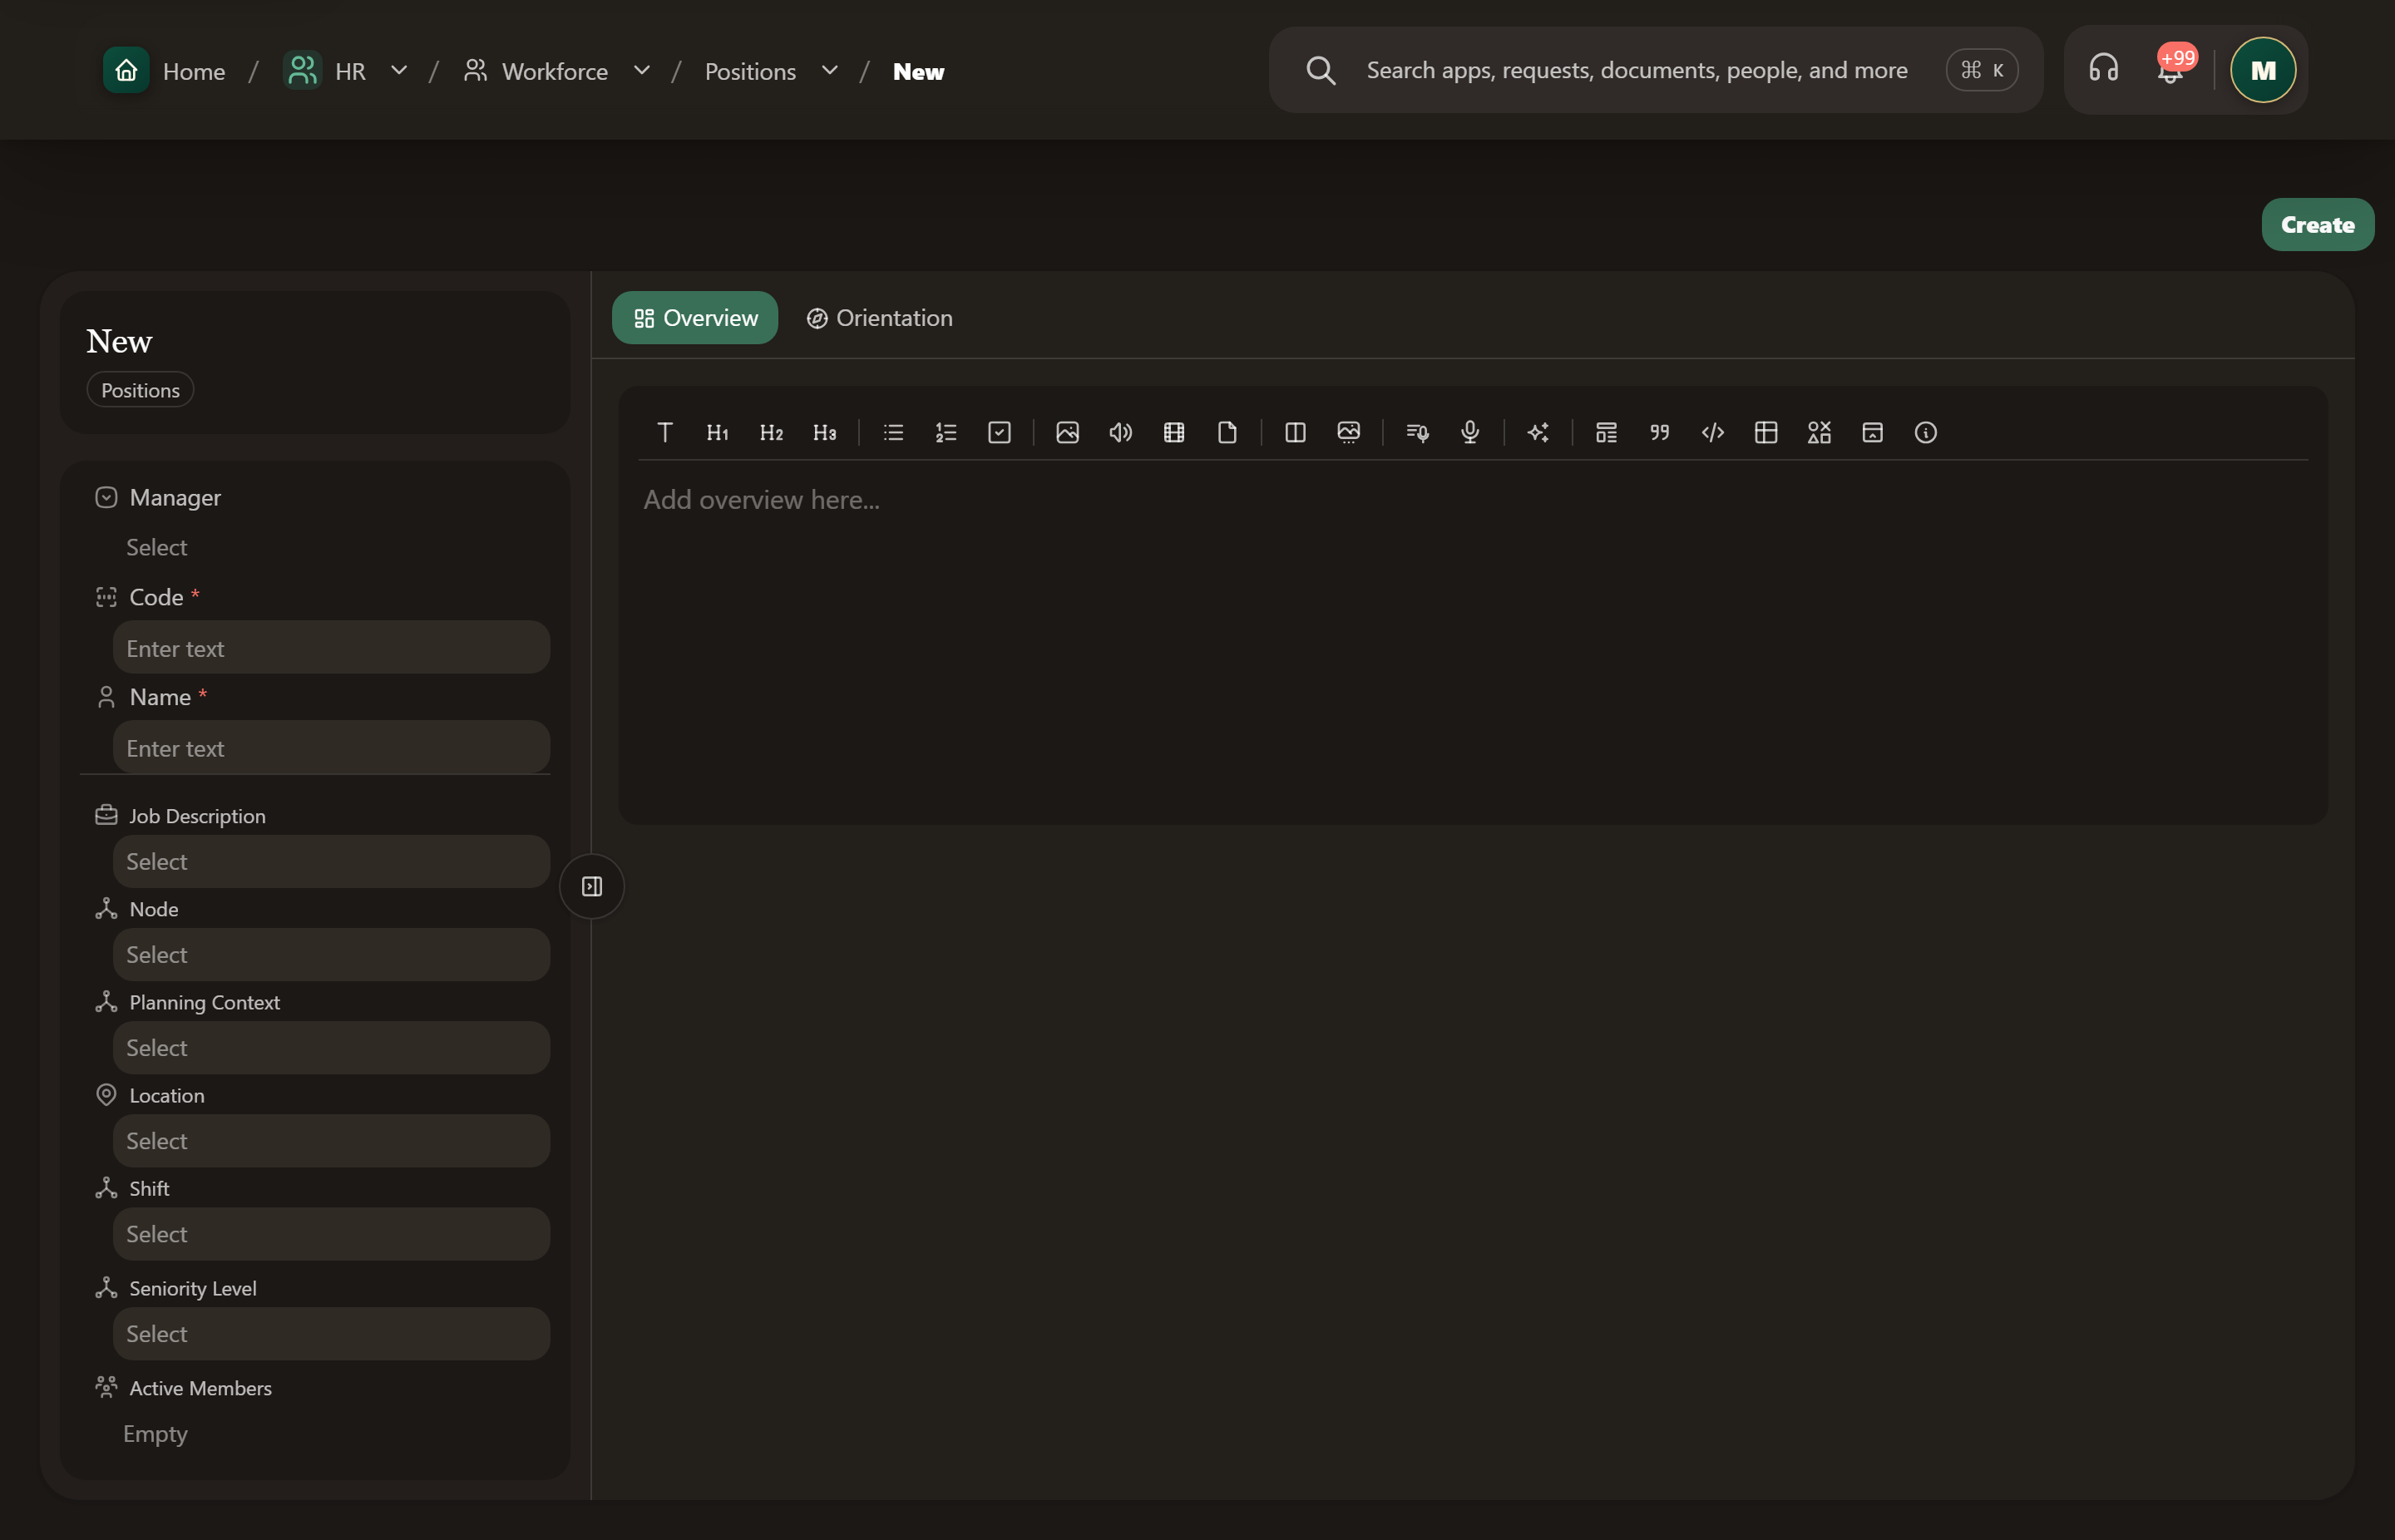
\includegraphics[width=0.95\linewidth]{figures/screens/ch02-position-fields-en.png}
\caption{Positions: Test form; not saved}
\label{fig:hr-feature-positions-screen}
\end{figure}

\begin{table}[H]
\centering
\caption{What do you record in a position?}
\label{tab:hr-feature-positions-data}
\rcZebra
\begin{tabularx}{\linewidth}{R{3.6cm} Y}
\rcHeaderRow
\thh{Field} & \thh{What do you add?}\\
Code and Name & \req{}; for example HZN-P-01 HR Manager.\\
Manager & The higher position; it builds the org chart tree.\\
Job Description & Duties and responsibilities, from the list of descriptions or a new one.\\
Node and Location & The unit and work site \opt{}.\\
Shift and Seniority Level & The job's working time and its grade in the salary scale \opt{}.\\
Planning Context & A plan, project or program the job belongs to \opt{}.\\
\end{tabularx}
\end{table}

\subsection{What can you do?}

\begin{itemize}
  \item “Tree” view: search positions, codes or people, expand or collapse, and “Show only this branch”.
  \item Each tree card shows the holder or “Vacant”, and the number of reports.
  \item The system shows the active members of the position \gen{}.
\end{itemize}

\begin{figure}[H]
\centering
\begin{tikzpicture}[node distance=0.5cm,stepBox/.append style={minimum width=6.5cm,text width=6.1cm,minimum height=0.8cm}]
  \node[stepBox] (a) {Define the job};
  \node[stepBox,below=of a] (b) {Choose unit and location};
  \node[stepBox,below=of b] (c) {Assign the employee};
  \draw[flowsTo] (a) -- (b);
  \draw[flowsTo] (b) -- (c);
\end{tikzpicture}
\rclegend
\caption{Steps of use; arrows do not mean automatic processing}
\label{fig:hr-feature-positions-flow}
\end{figure}

\subsection{Try it and check}

\begin{enumerate}
  \item Prepare the unit and location if you want to link them. Open Positions and search for the job.
  \item Add “HR Manager” with code HZN-P-01, choose the HR unit and Head Office Damascus, then save.
\end{enumerate}

\textbf{Check:} reopen the position and check its links, then open the tree. Creating the position does not assign Sarah to it.

\begin{figure}[H]
\centering
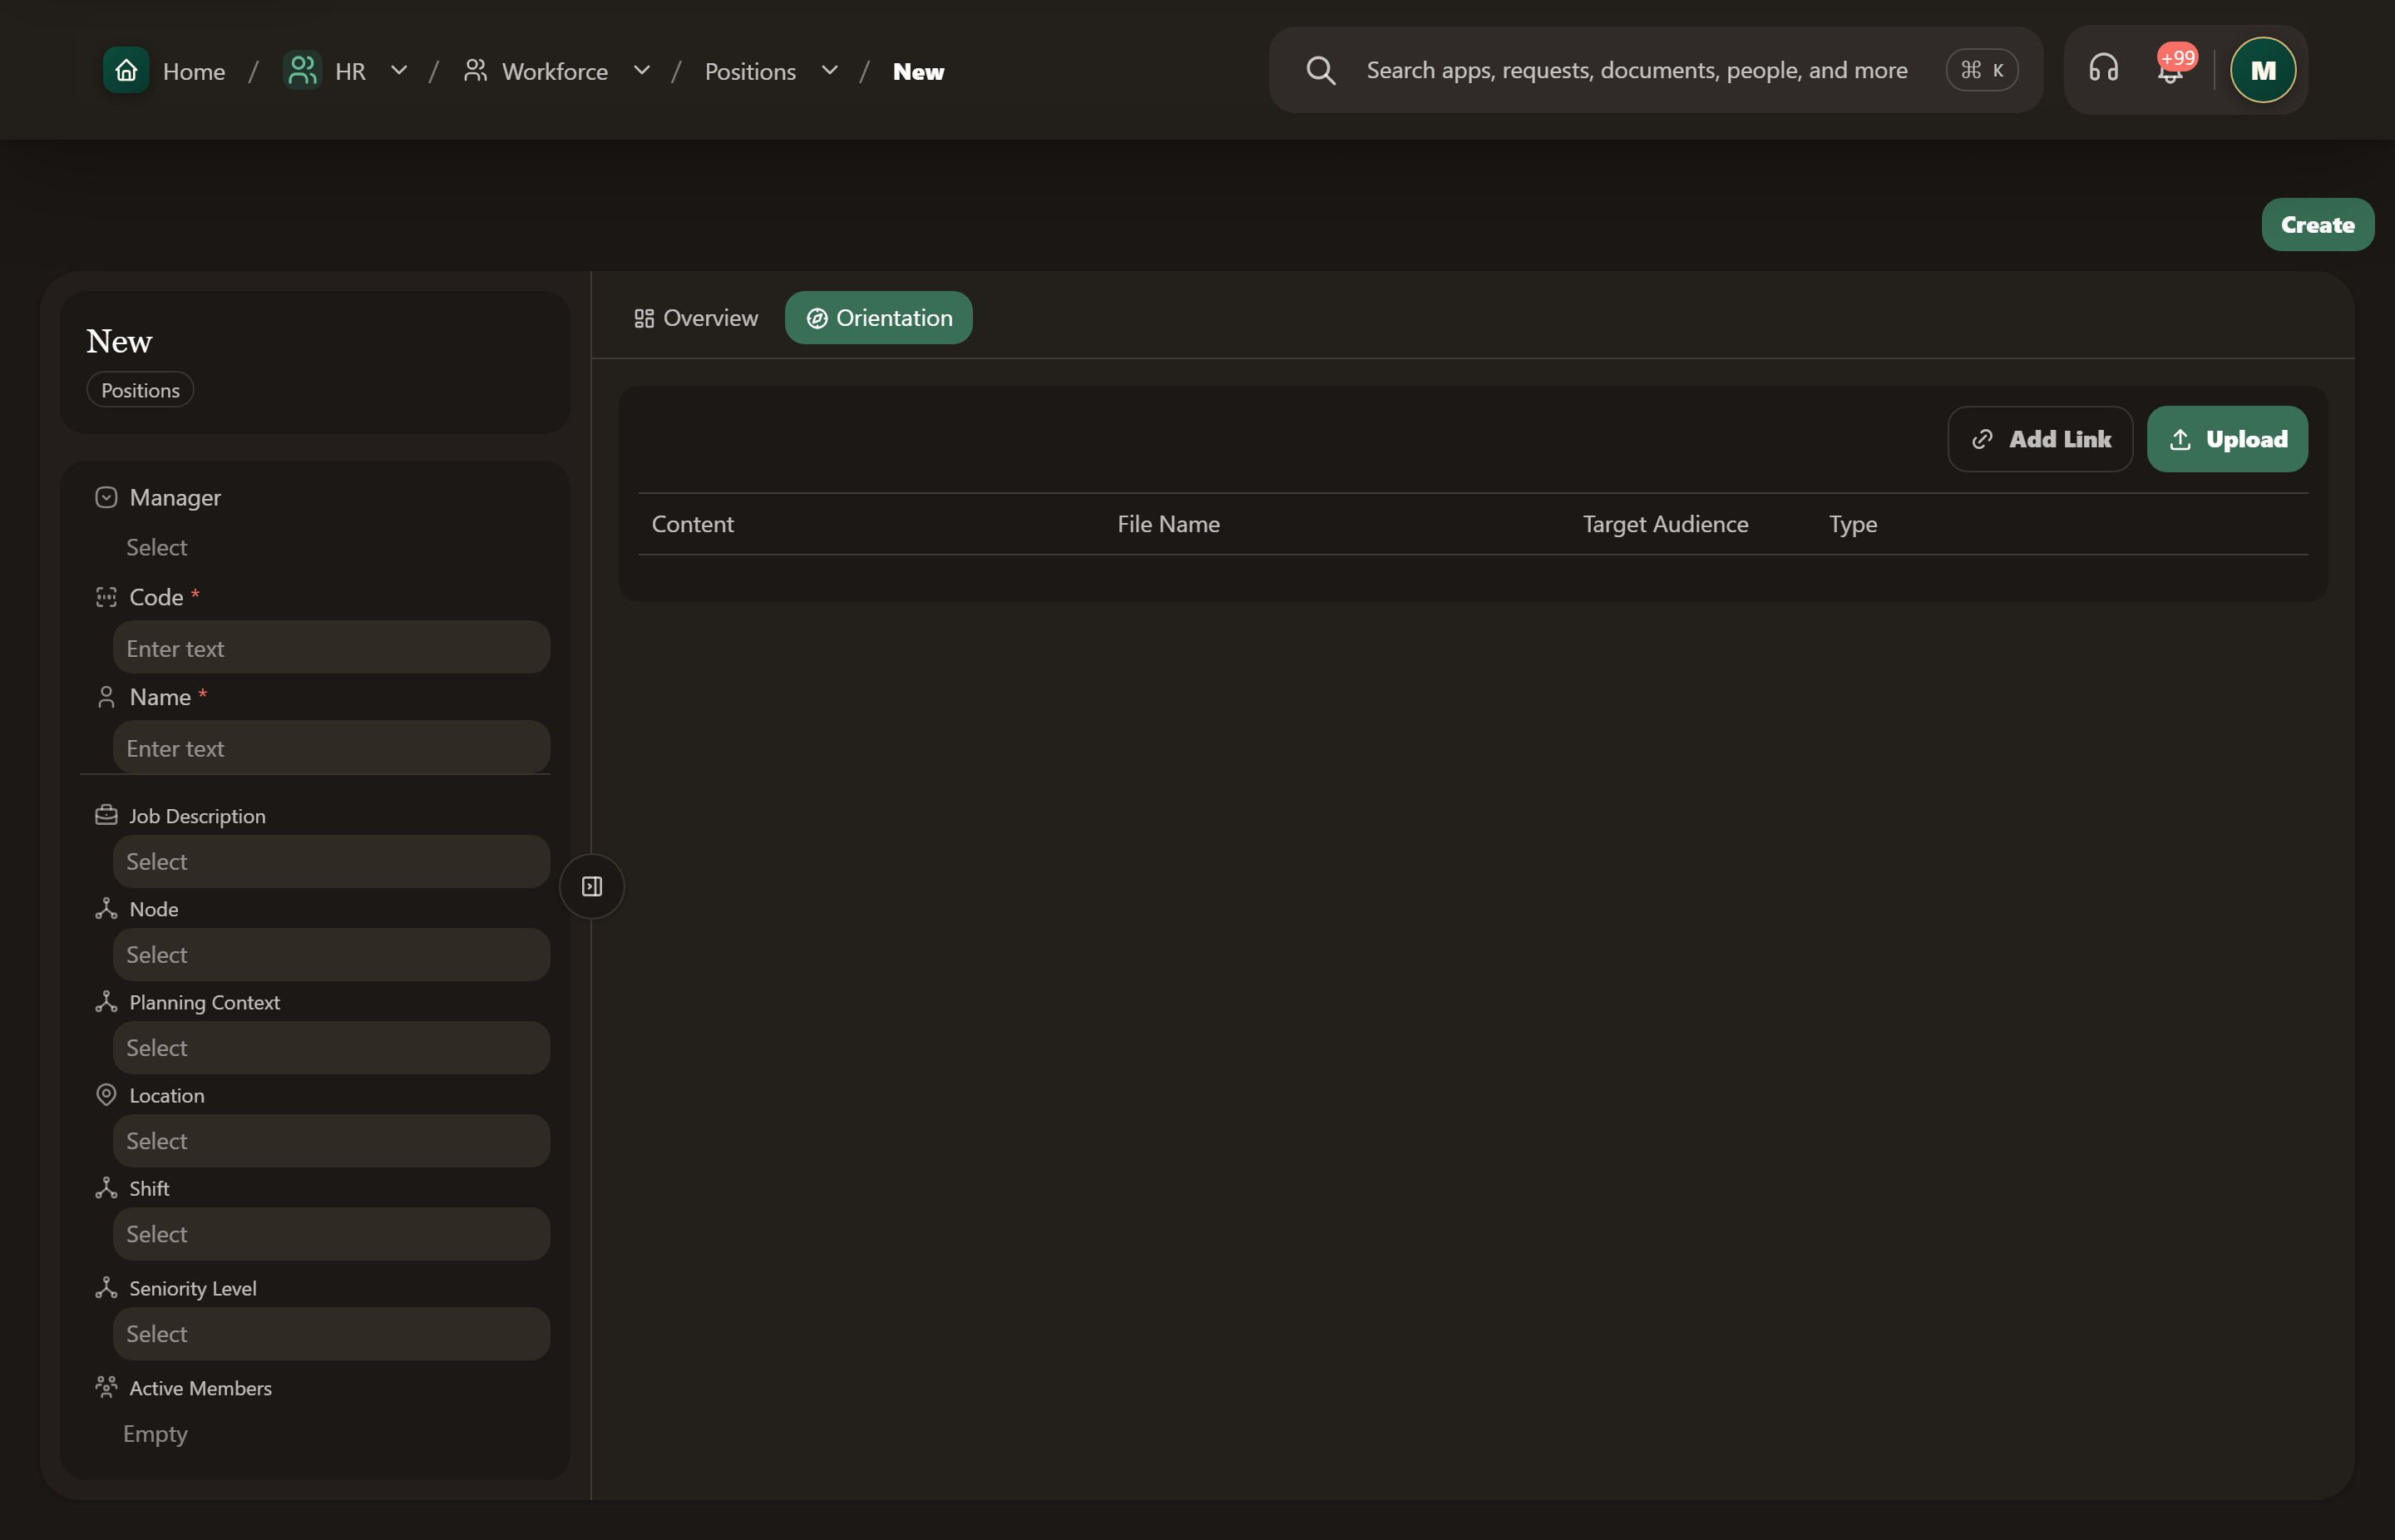
\includegraphics[width=0.95\linewidth]{figures/screens/ch02-position-fields-tab2-en.png}
\caption{Orientation tab in full; unsaved form}
\label{fig:hr-positions-fulltab1}
\end{figure}

\clearpage
\section{Assignments}
\label{sec:hr-feature-assignments}

An assignment records who holds the position, since when, and on which contract, salary and shift.

\textbf{When is it useful?} When Sarah joins or moves to another job; her jobs and dates stay separate from her personal file. \textbf{Open:} HR / Workforce / Assignments.

\begin{figure}[H]
\centering
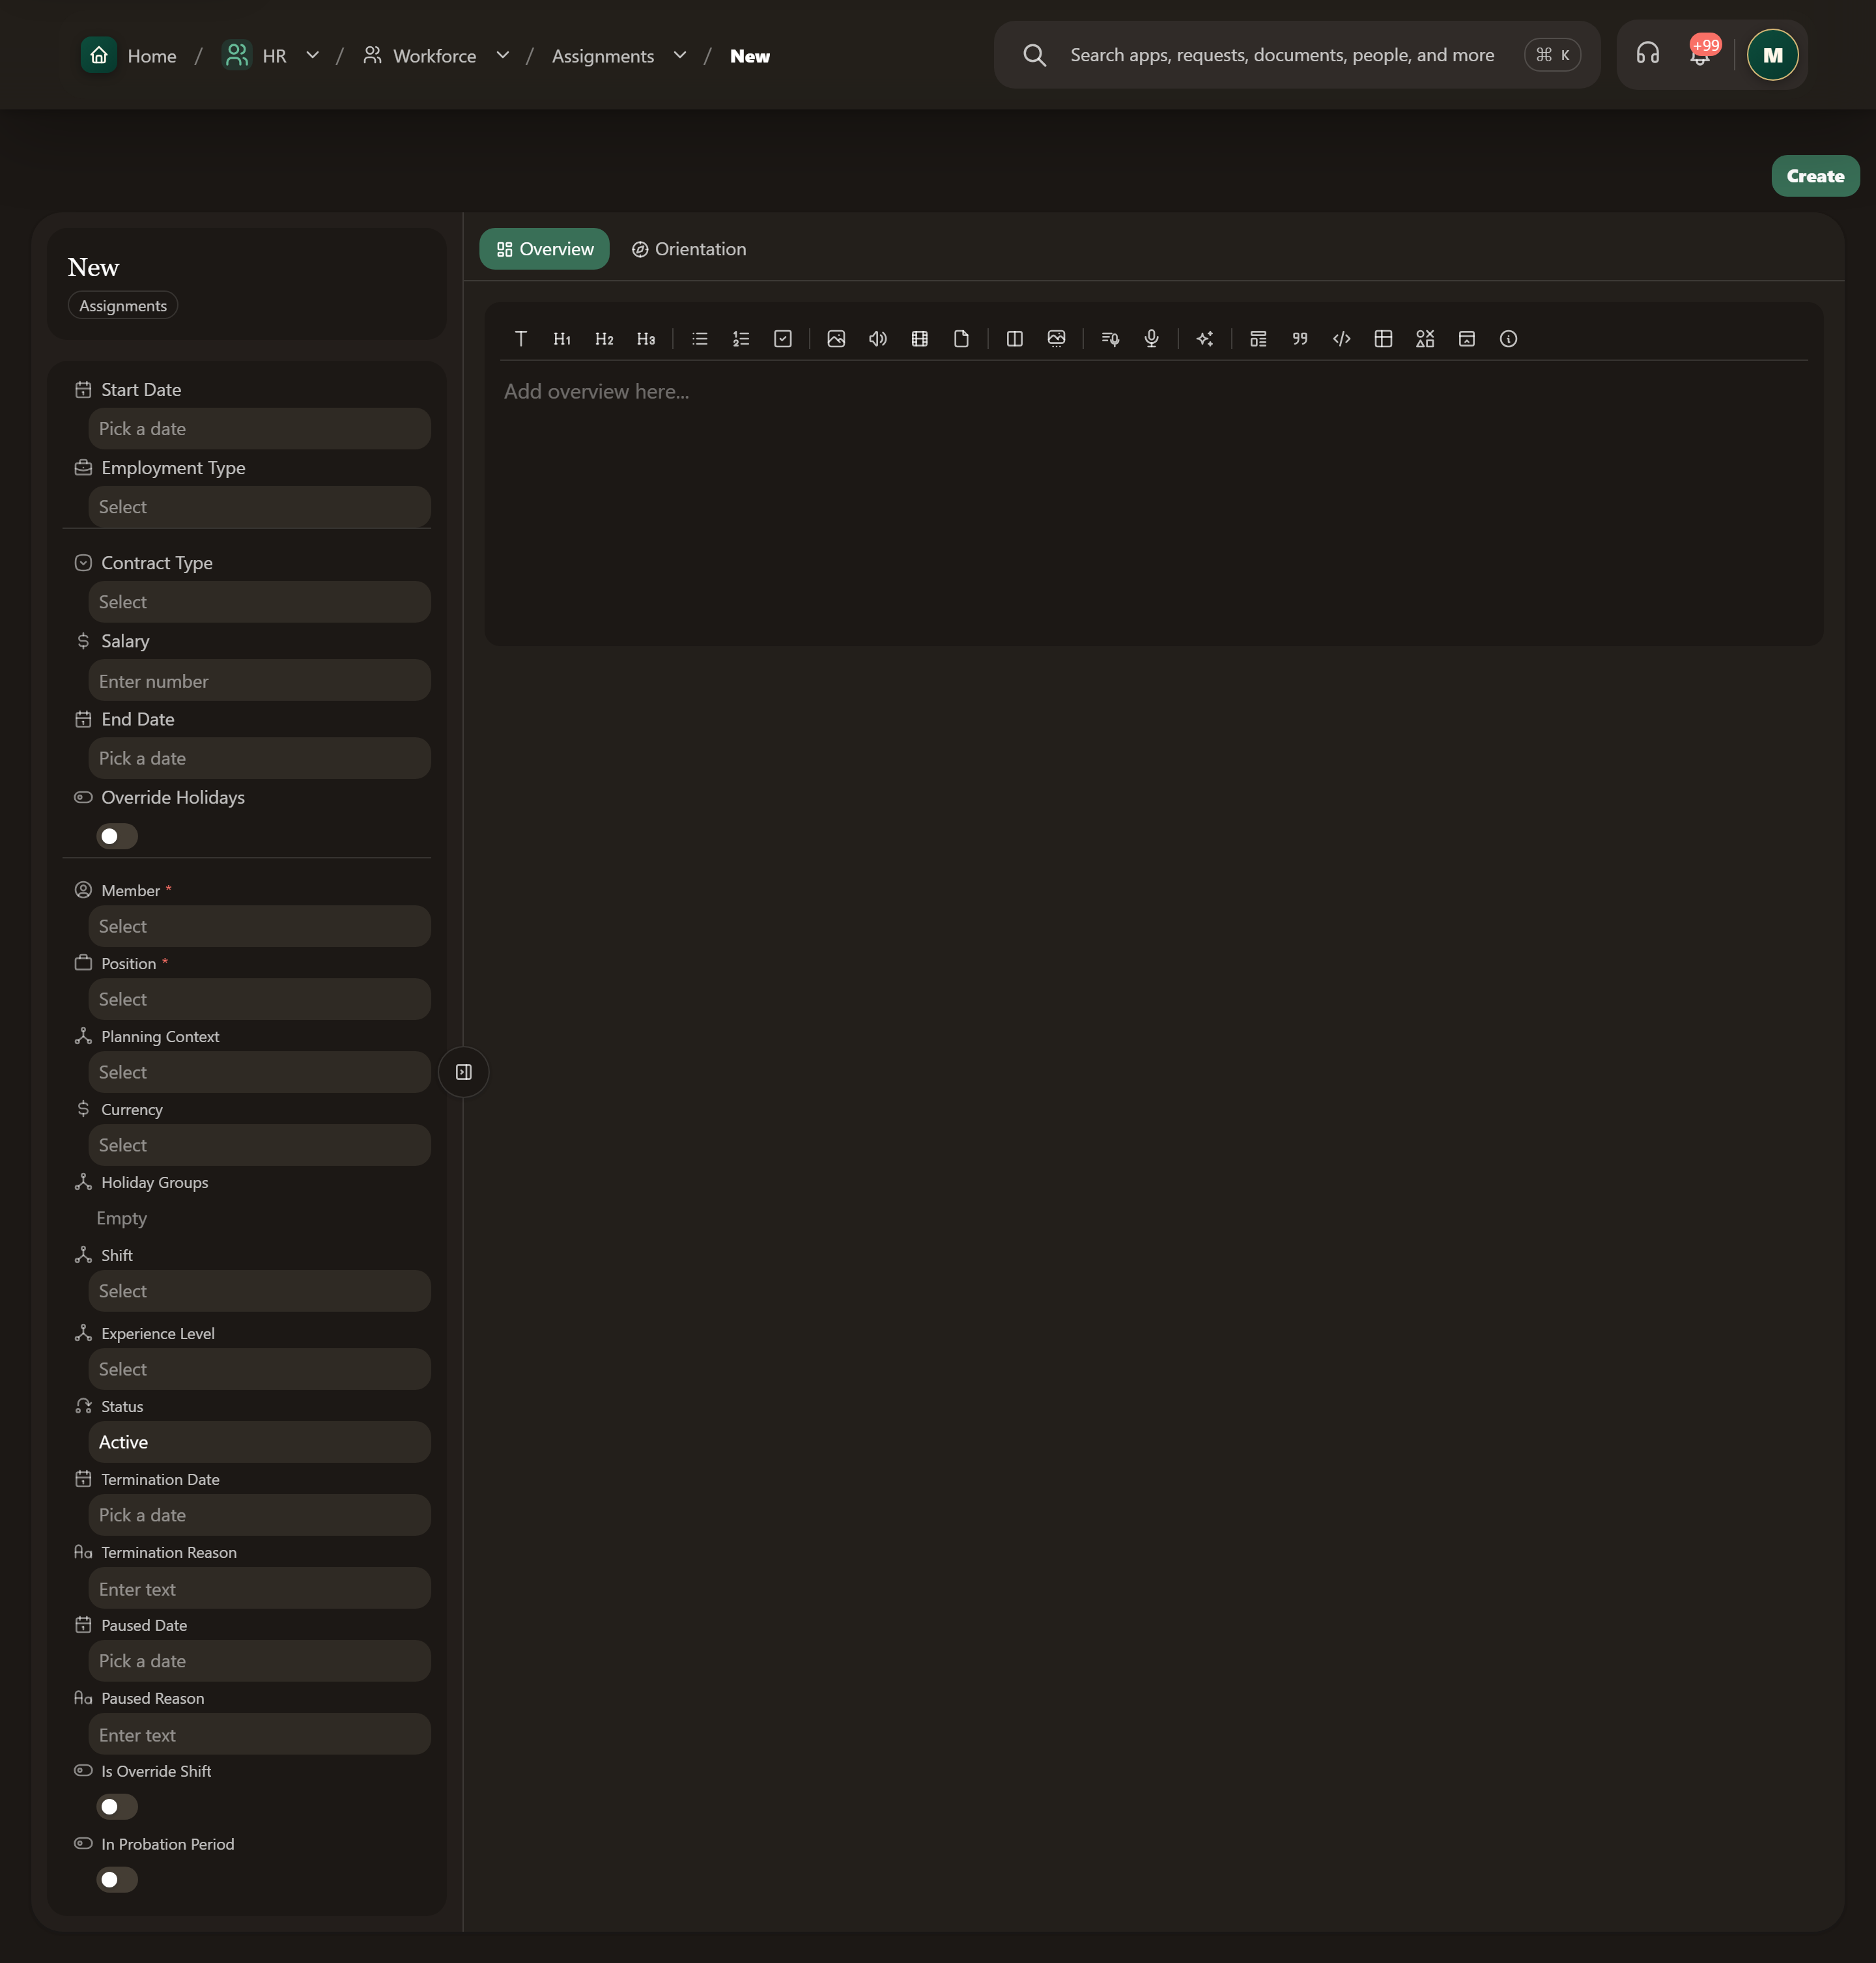
\includegraphics[width=0.95\linewidth]{figures/screens/ch02-assignment-fields-en.png}
\caption{Assignments: Test form; not saved}
\label{fig:hr-feature-assignments-screen}
\end{figure}

\begin{table}[H]
\centering
\caption{What do you record in an assignment?}
\label{tab:hr-feature-assignments-data}
\rcZebra
\begin{tabularx}{\linewidth}{R{3.6cm} Y}
\rcHeaderRow
\thh{Group} & \thh{What do you add?}\\
Person and job & Member \req{} and Position \req{}.\\
Contract & Employment Type: Employee, Contractor, Volunteer, Intern, Acting As, On Demand. Contract Type: Permanent, Fixed Term, Temporary.\\
Period & Start and end date, and the probation period with its end date.\\
Pay & Salary, currency and experience level.\\
Time & Shift and its override, holiday groups and their override.\\
Status & Active, Paused, Terminated, Finished; with the pause or termination date and reason.\\
\end{tabularx}
\end{table}

\subsection{What can you do?}

\begin{itemize}
  \item View the list as a table, a kanban by status, or a calendar and timeline by start and end dates.
  \item Start an assignment from the member file with “Add Assignment”.
  \item Saving updates the member's active positions and the position's holders \gen{}.
\end{itemize}

\begin{figure}[H]
\centering
\begin{tikzpicture}[node distance=0.5cm,stepBox/.append style={minimum width=6.5cm,text width=6.1cm,minimum height=0.8cm}]
  \node[stepBox] (a) {Prepare member and position};
  \node[stepBox,below=of a] (b) {Save the assignment};
  \node[stepBox,below=of b] (c) {Review period\\and shift};
  \draw[flowsTo] (a) -- (b);
  \draw[flowsTo] (b) -- (c);
\end{tikzpicture}
\rclegend
\caption{Steps of use; arrows do not mean automatic processing}
\label{fig:hr-feature-assignments-flow}
\end{figure}

\subsection{Try it and check}

\begin{enumerate}
  \item Prepare Sarah's record and the HR Manager position, or search for them.
  \item Add an assignment: Sarah, the position, “Employee”, “Permanent”, and the actual start date. Keep the status “Active” and save.
\end{enumerate}

\textbf{Check:} reopen it and check the person, position, period and status. When the job changes, end the old assignment and add a new one; do not create another member.

\begin{figure}[H]
\centering
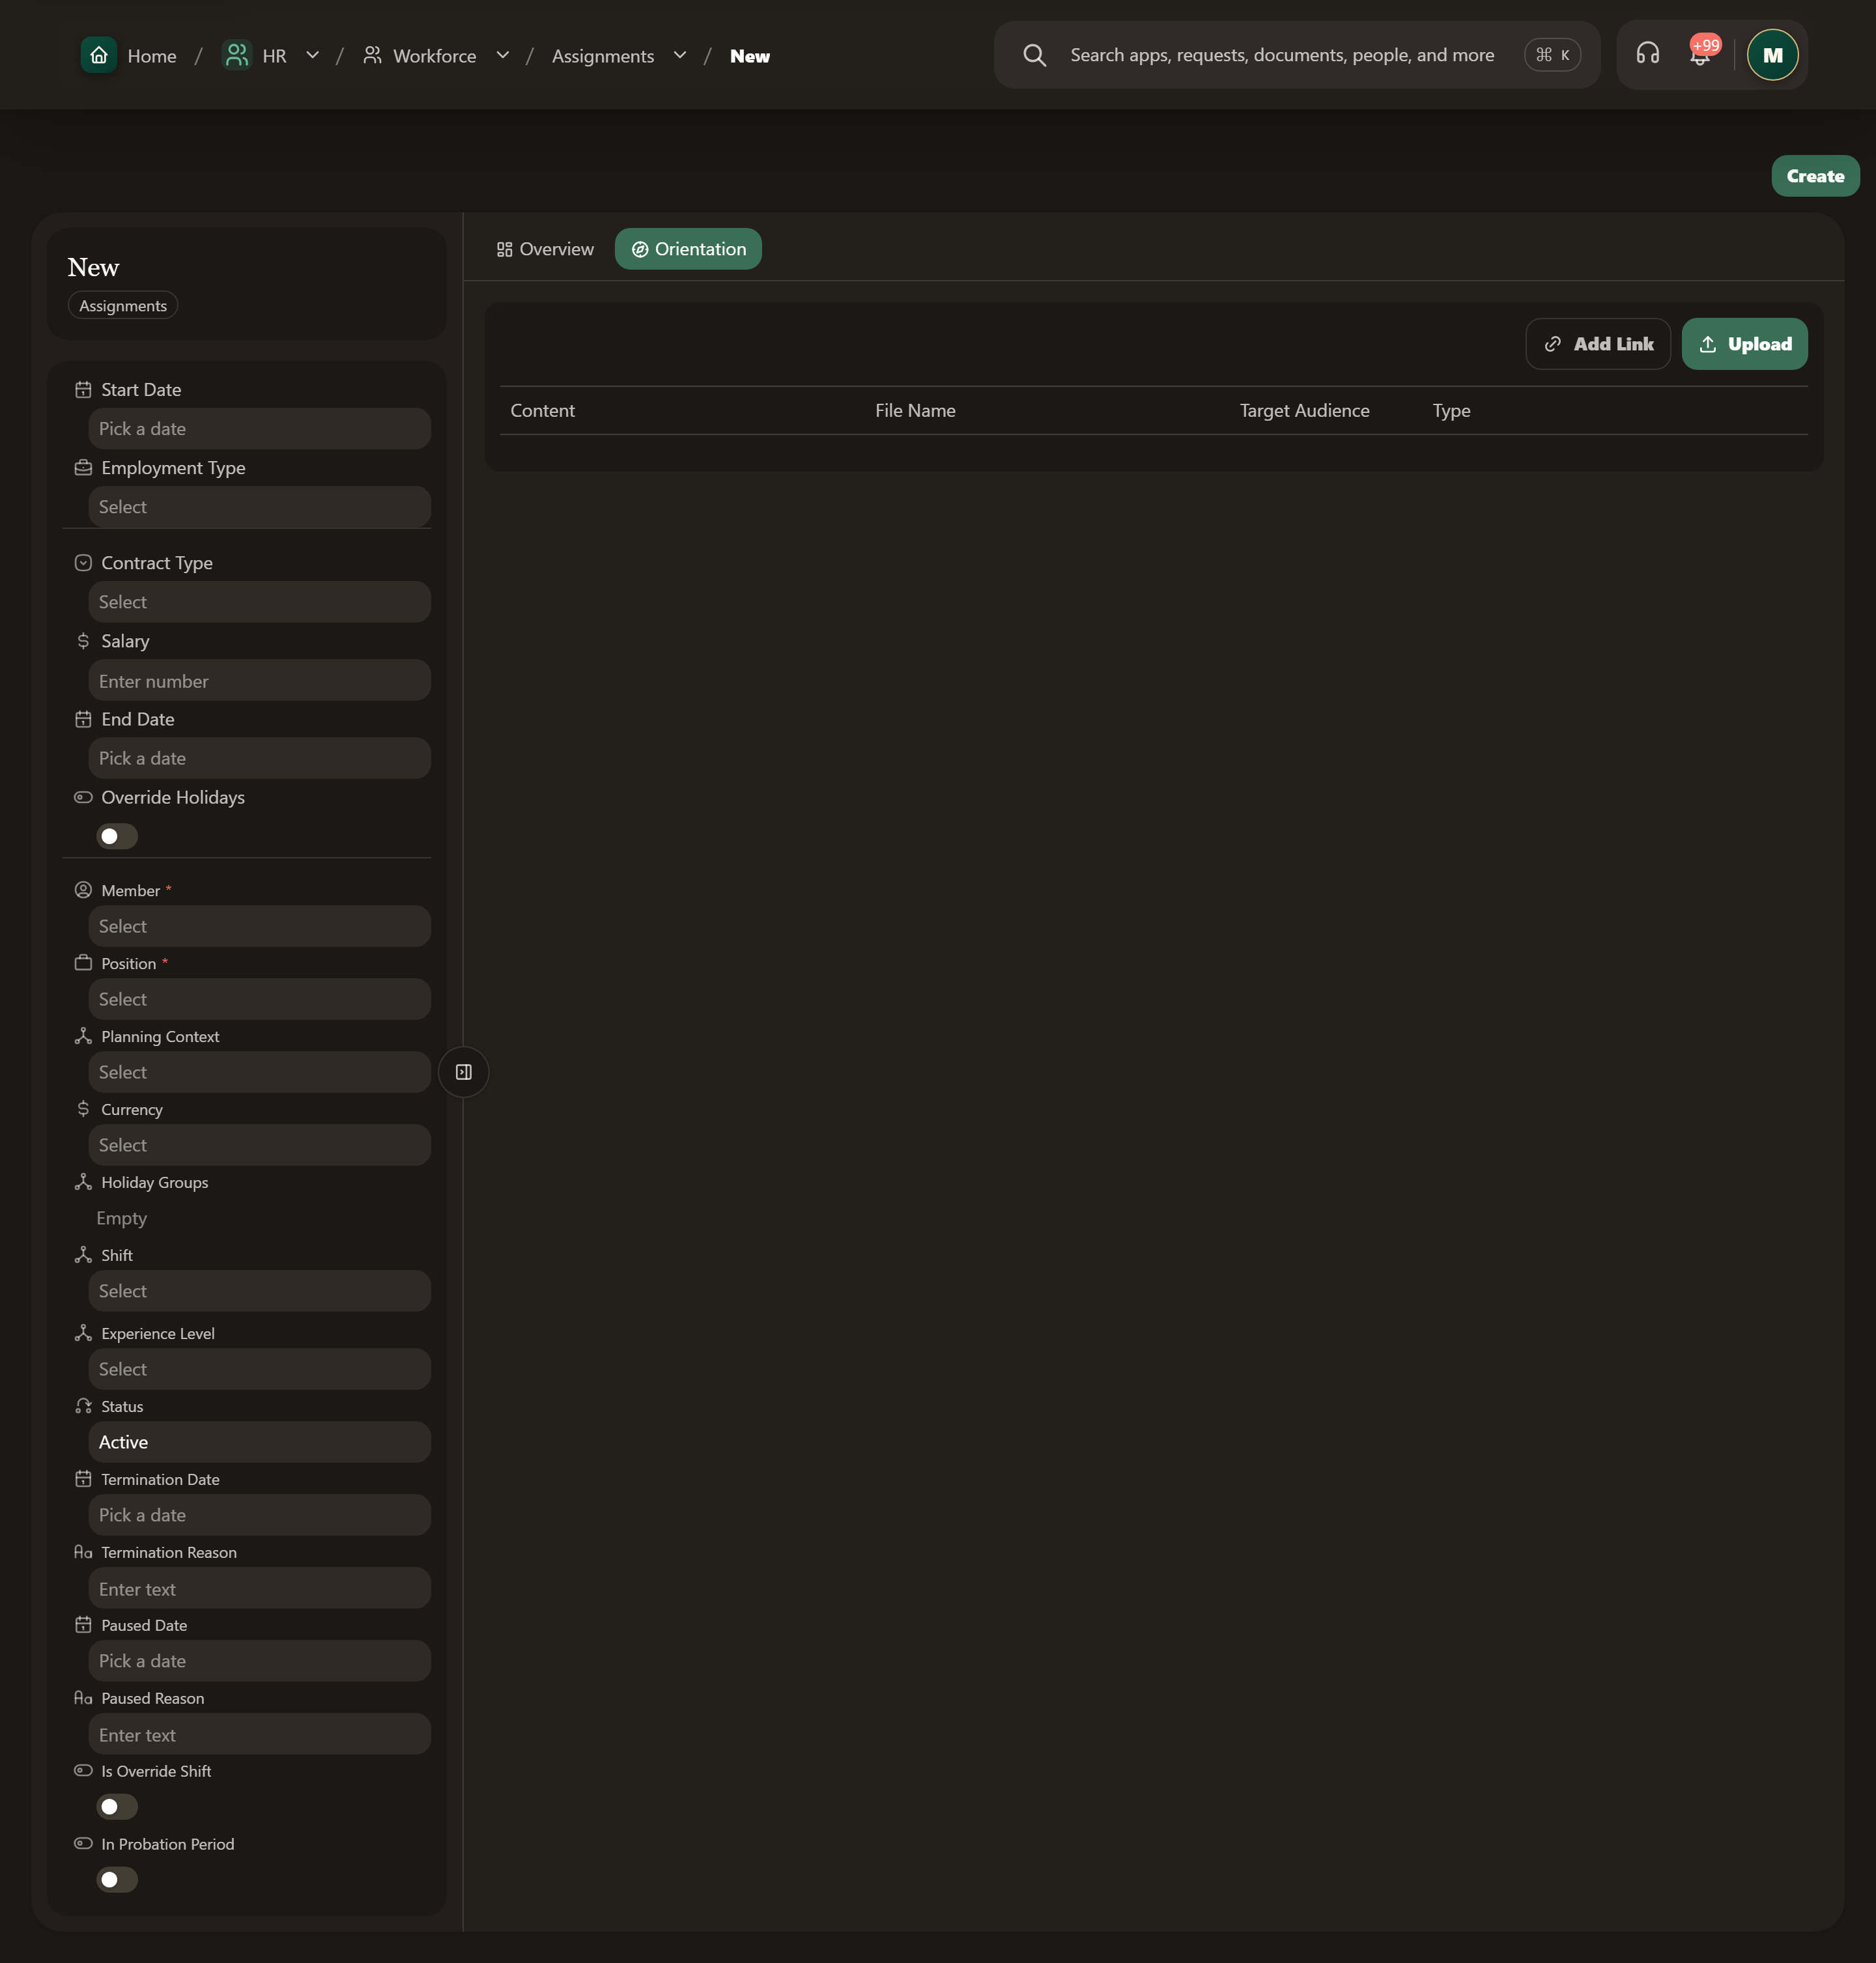
\includegraphics[width=0.95\linewidth]{figures/screens/ch02-assignment-fields-tab2-en.png}
\caption{Orientation tab in full; unsaved form}
\label{fig:hr-assignments-fulltab1}
\end{figure}

\clearpage
\section{Nodes}
\label{sec:hr-feature-nodes}

A node is a department or division. The “Parent” field places it in the structure tree. It is the job's reporting unit, not a work address.

\textbf{When is it useful?} It keeps the structure clear as the team grows. At Horizon, HR belongs to General Management. \textbf{Open:} HR / Core / Nodes.

\begin{figure}[H]
\centering
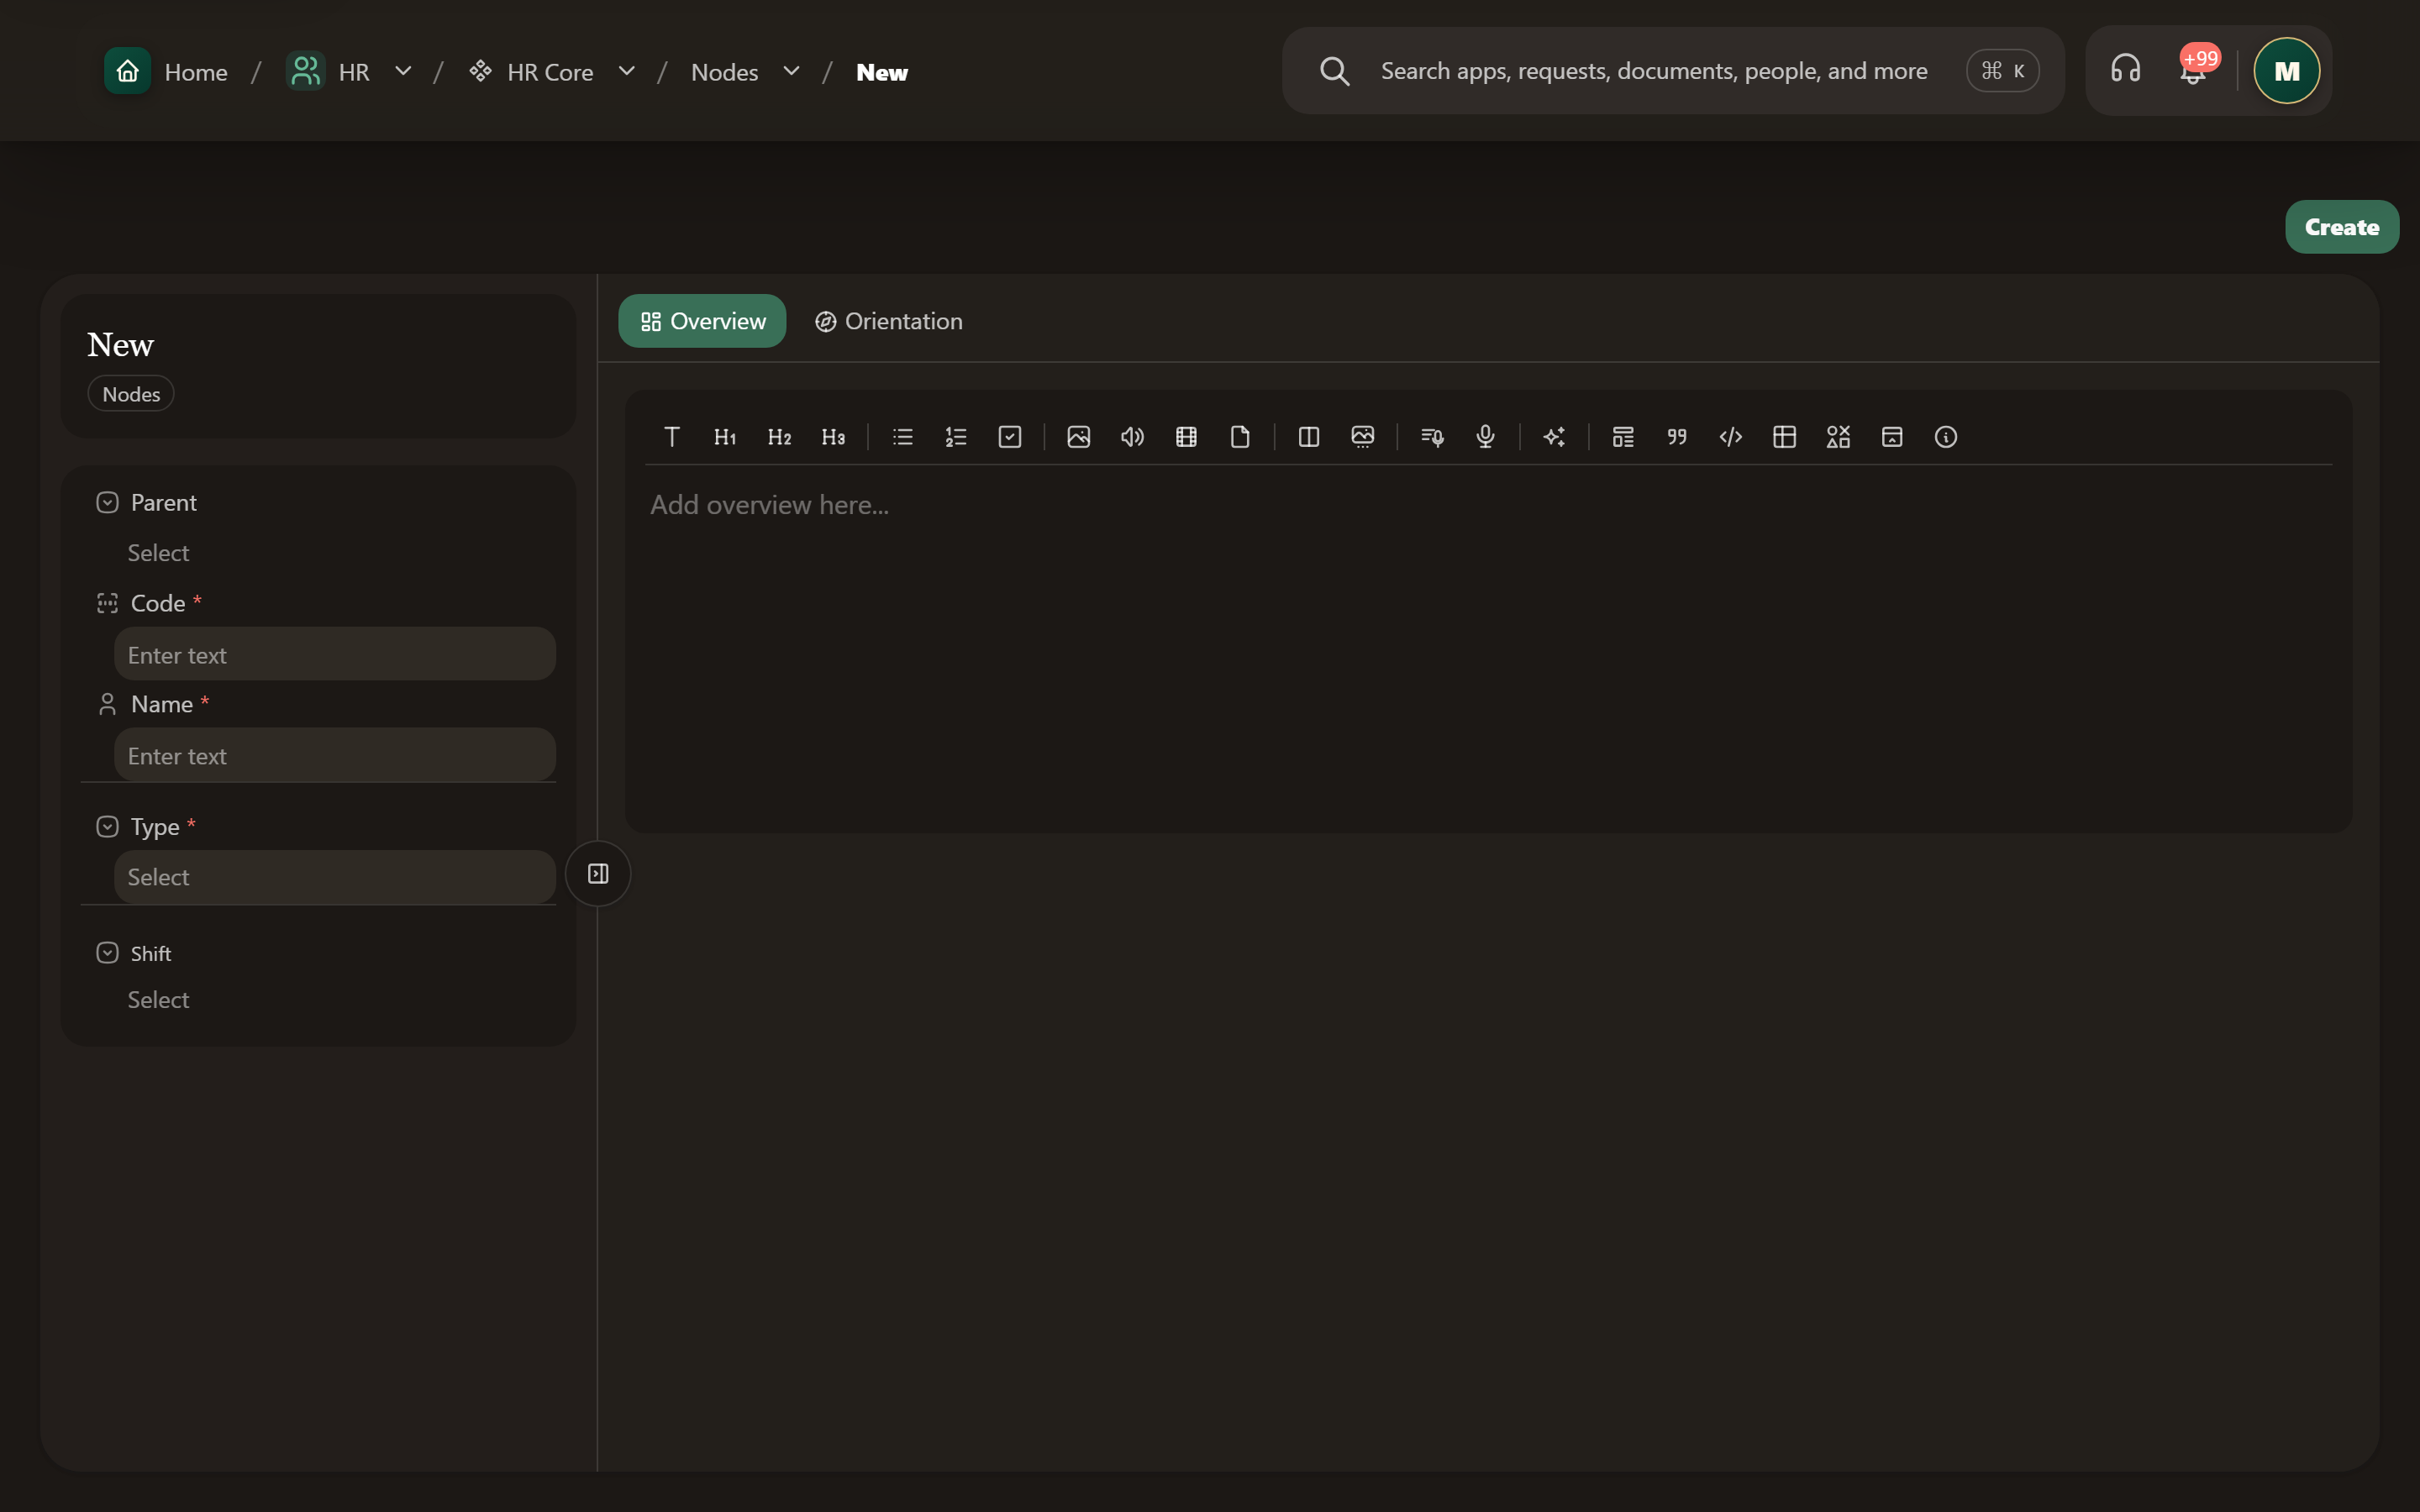
\includegraphics[width=0.95\linewidth]{figures/screens/ch02-node-fields-en.png}
\caption{Nodes: Test form; not saved}
\label{fig:hr-feature-nodes-screen}
\end{figure}

\begin{table}[H]
\centering
\caption{What do you record in a node?}
\label{tab:hr-feature-nodes-data}
\rcZebra
\begin{tabularx}{\linewidth}{R{3.6cm} Y}
\rcHeaderRow
\thh{Field} & \thh{What do you add?}\\
Code, Name and Type & \req{}; types are defined by the organization's administrator, such as division or department.\\
Parent & The parent unit, such as HZN-GM for HR.\\
Shift & Inherited from the parent unit, or overridden with its own shift.\\
Overview and Orientation & A description of the unit, and material that introduces it to new employees.\\
\end{tabularx}
\end{table}

\subsection{What can you do?}

\begin{itemize}
  \item “Tree” view with search; each card shows positions, staff and vacancies.
  \item “With Descendants” or “Without Descendants”: whether counts include sub-units.
  \item “Override” the inherited shift, and “Reset” to restore inheritance.
\end{itemize}

\begin{figure}[H]
\centering
\begin{tikzpicture}[node distance=0.5cm,stepBox/.append style={minimum width=6.5cm,text width=6.1cm,minimum height=0.8cm}]
  \node[stepBox] (a) {Create General\\Management};
  \node[stepBox,below=of a] (b) {Add HR under it};
  \node[stepBox,below=of b] (c) {Link the HR Manager\\position};
  \draw[flowsTo] (a) -- (b);
  \draw[flowsTo] (b) -- (c);
\end{tikzpicture}
\rclegend
\caption{Steps of use; arrows do not mean automatic processing}
\label{fig:hr-feature-nodes-flow}
\end{figure}

\subsection{Try it and check}

\begin{enumerate}
  \item Open Nodes. If General Management does not exist, add it with code HZN-GM, choose its type and save.
  \item Add “Human Resources” with code HZN-HR, choose the type, and General Management in “Parent”, then save.
\end{enumerate}

\textbf{Check:} open the tree and confirm HR sits under General Management. Linking a position to a unit is optional and does not replace Sarah's assignment.

\begin{figure}[H]
\centering
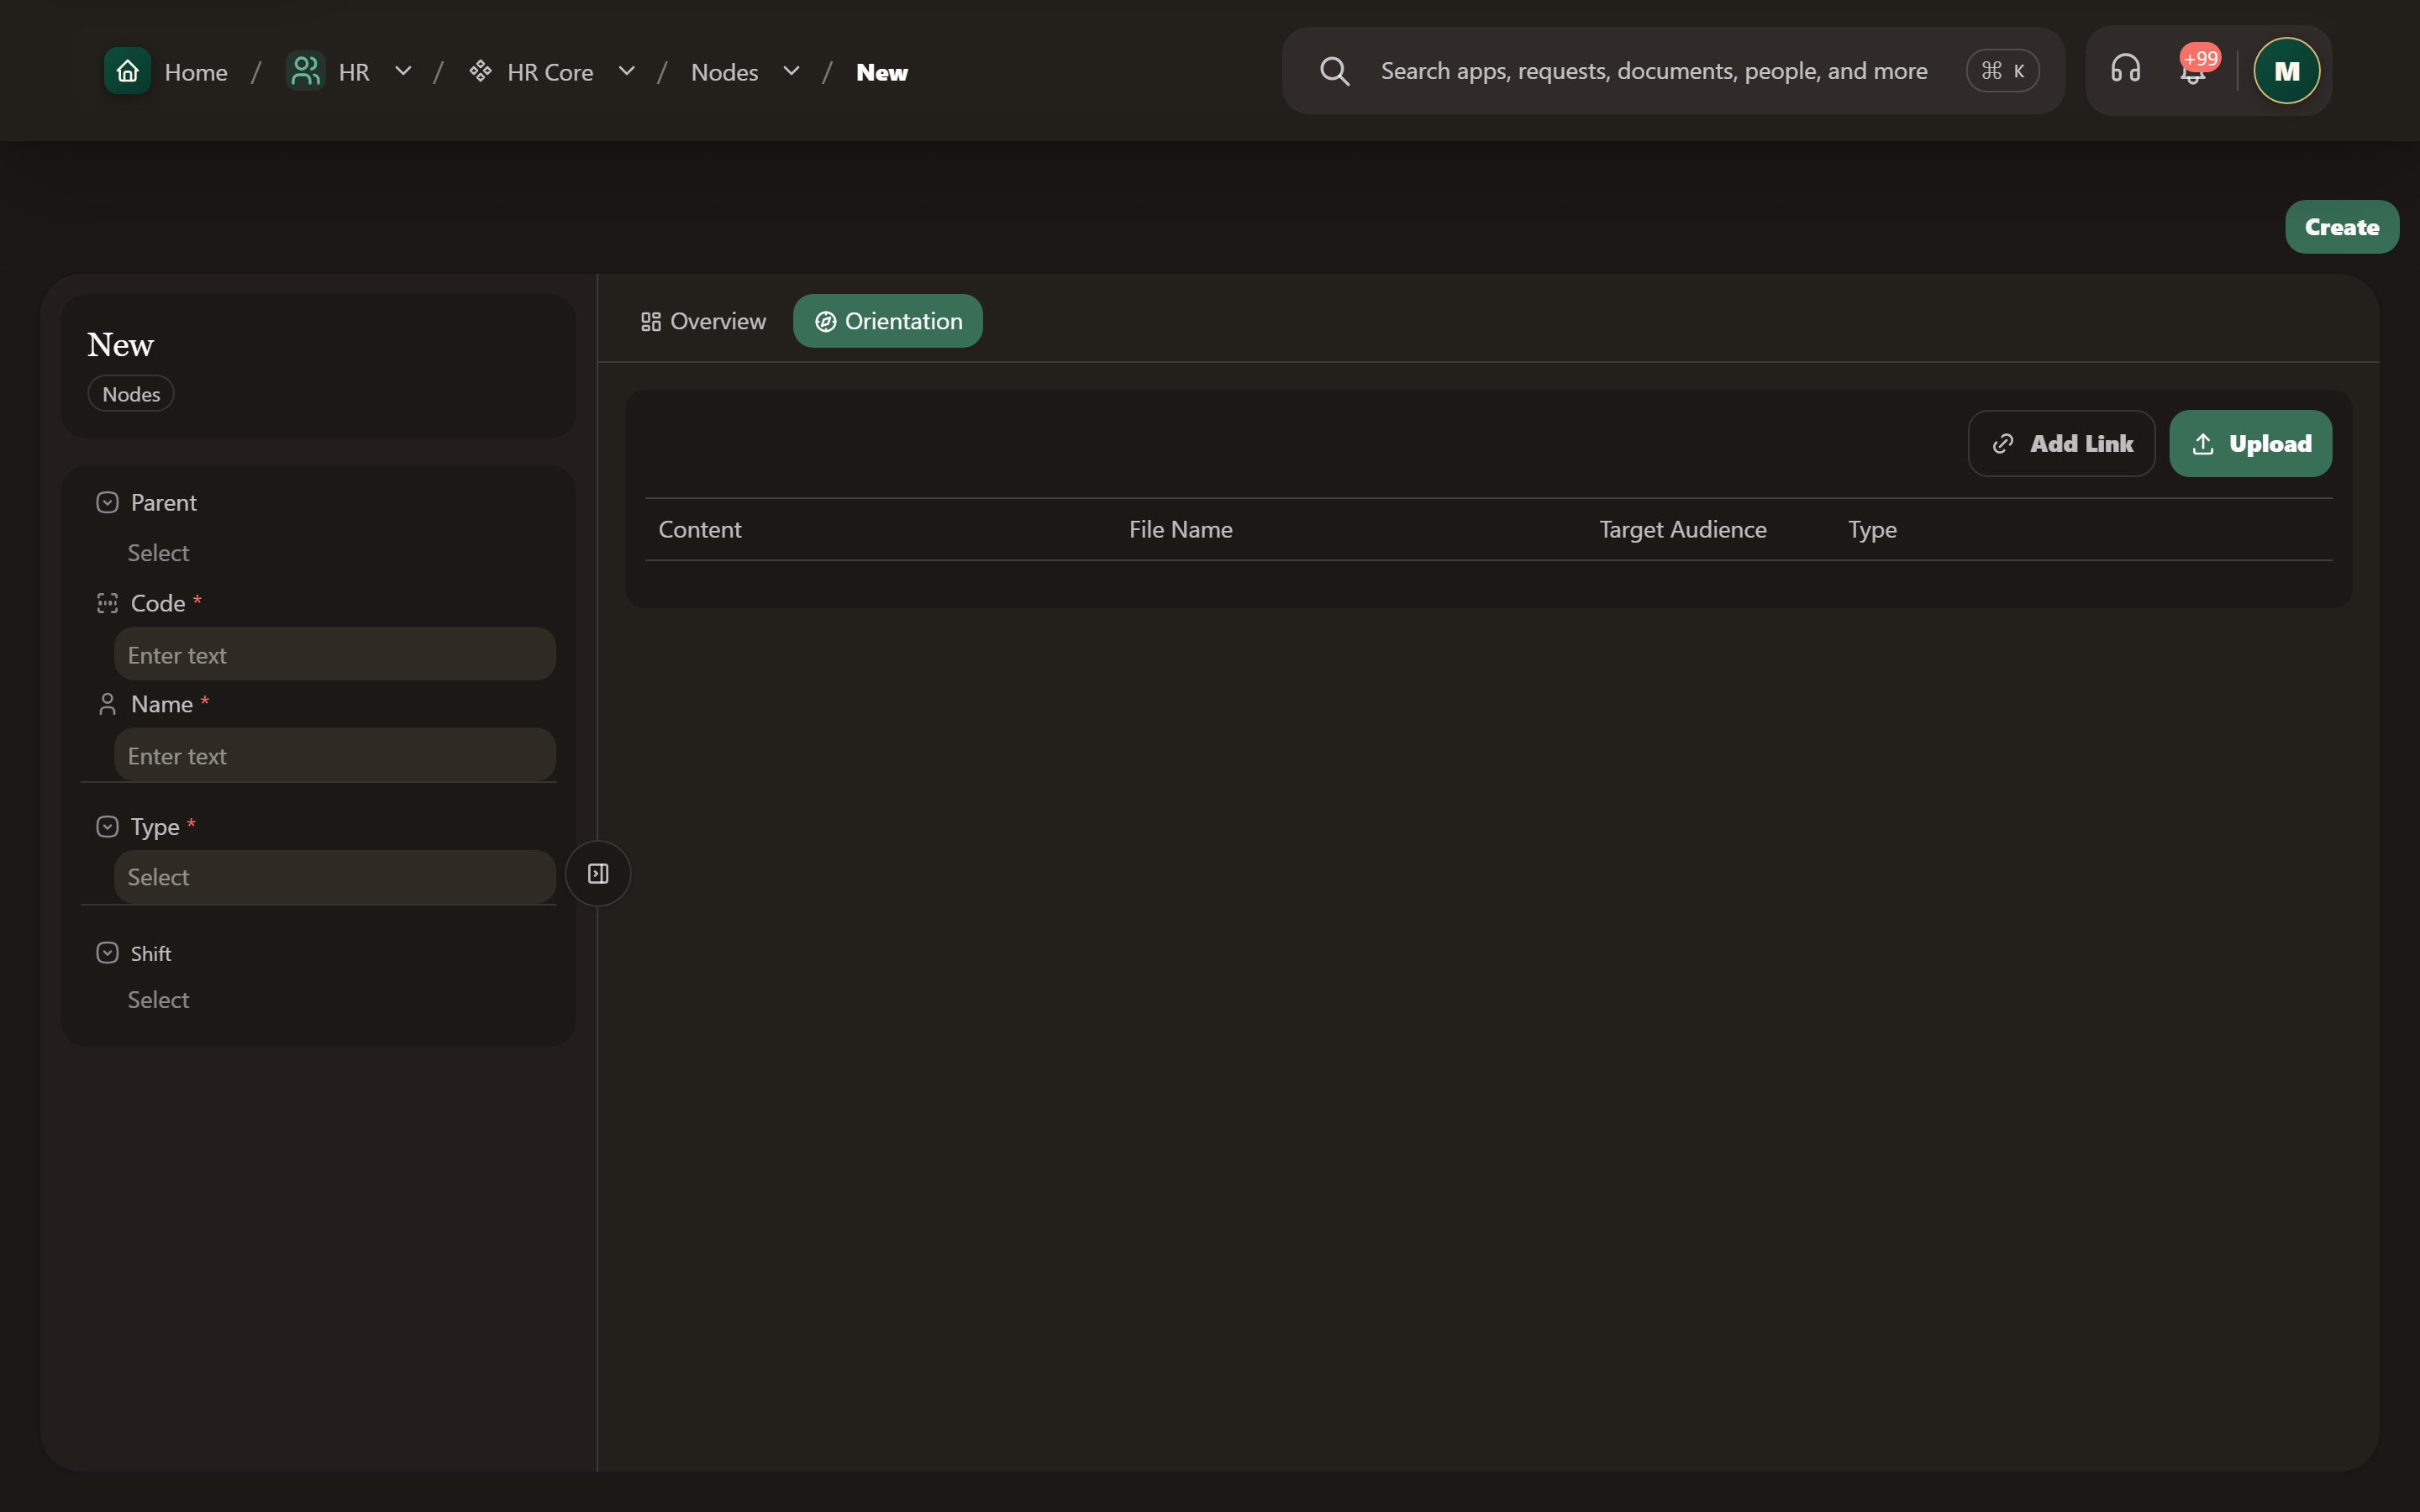
\includegraphics[width=0.95\linewidth]{figures/screens/ch02-node-fields-tab2-en.png}
\caption{Orientation tab in full; unsaved form}
\label{fig:hr-nodes-fulltab1}
\end{figure}

\clearpage
\section{Locations}
\label{sec:hr-feature-locations}

A location is a work site, such as an office or branch, with its address and map point. It can belong to another location.

\textbf{When is it useful?} It separates place from unit: two units in the Damascus office, or one unit across several sites. \textbf{Open:} HR / Core / Locations.

\begin{figure}[H]
\centering
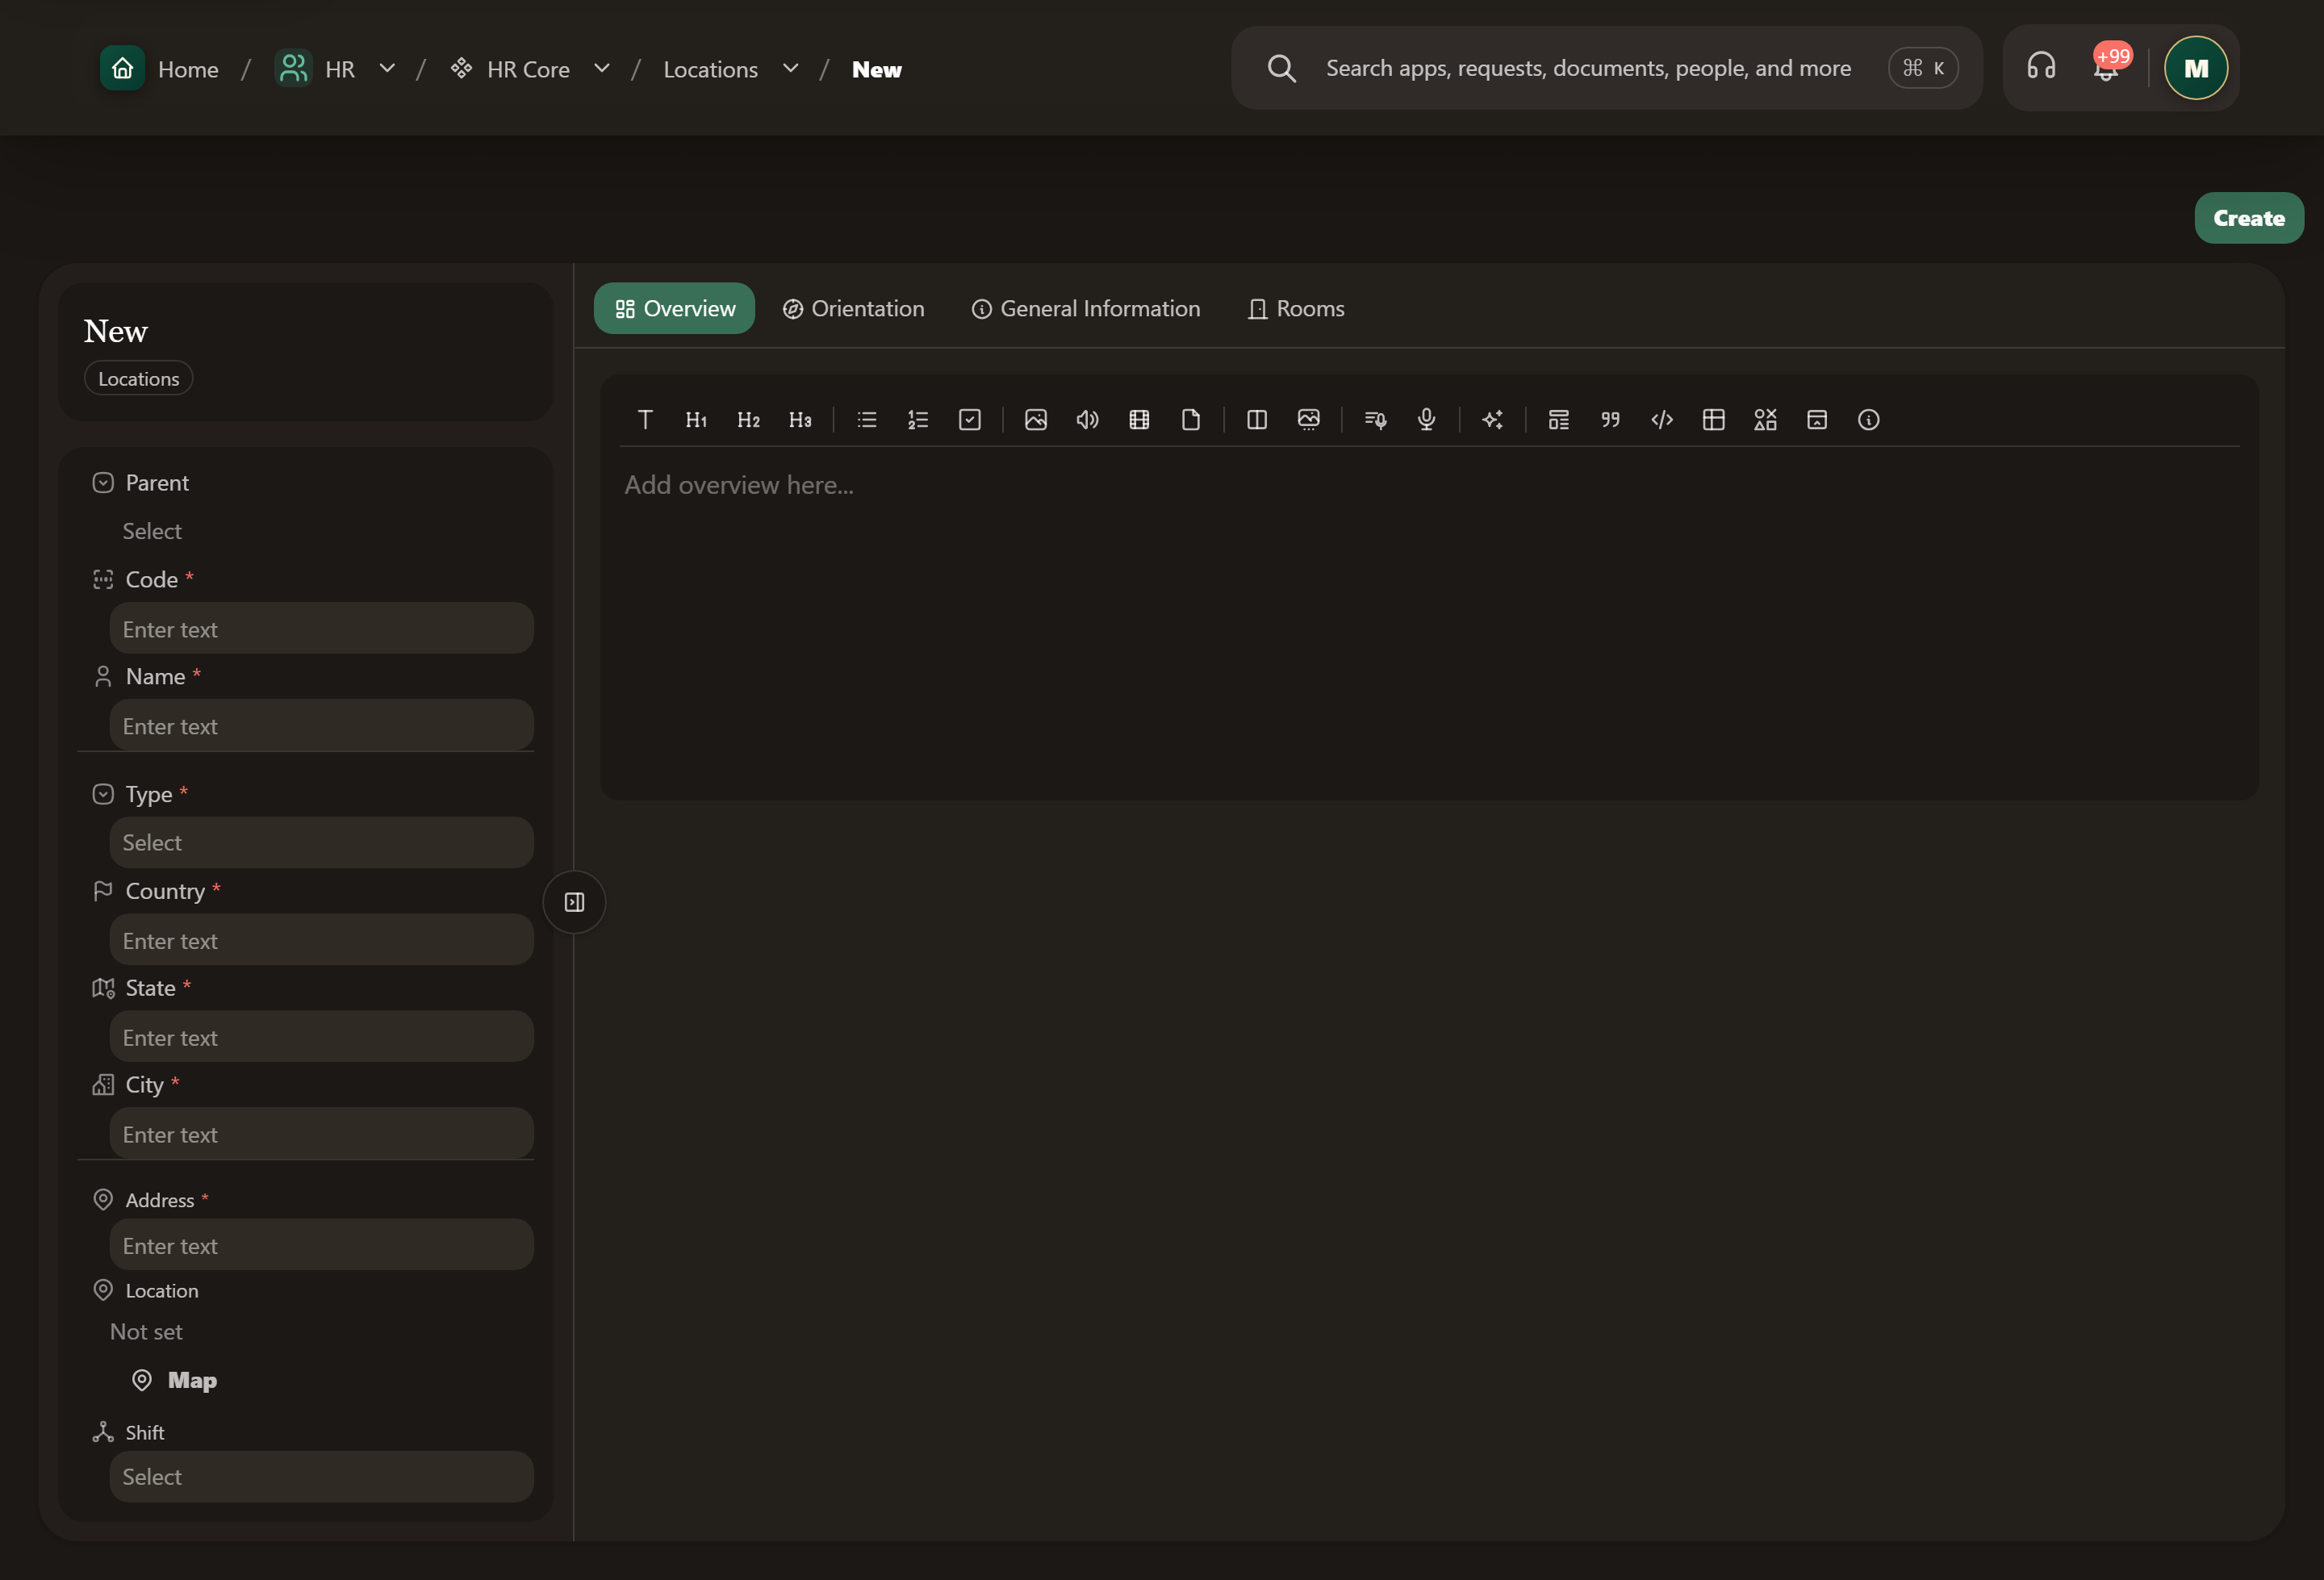
\includegraphics[width=0.95\linewidth]{figures/screens/ch02-location-fields-en.png}
\caption{Locations: Test form; not saved}
\label{fig:hr-feature-locations-screen}
\end{figure}

\begin{table}[H]
\centering
\caption{What do you record in a location?}
\label{tab:hr-feature-locations-data}
\rcZebra
\begin{tabularx}{\linewidth}{R{3.6cm} Y}
\rcHeaderRow
\thh{Tab or field} & \thh{What do you add?}\\
Main & Code, Name and Type \req{}; parent location and shift \opt{}.\\
Address & Country, State, City and Address \req{}, and a point on the map.\\
General Information & Ownership, area in square metres, contract file.\\
Rooms & Rooms: type, code, floor, capacity and area, and equipment such as a screen or projector.\\
\end{tabularx}
\end{table}

\subsection{What can you do?}

\begin{itemize}
  \item “Map” view with location pins, or the “Tree” of sub-locations.
  \item Search by name, code, city or address, and filter by type and country.
\end{itemize}

\begin{figure}[H]
\centering
\begin{tikzpicture}[node distance=0.5cm,stepBox/.append style={minimum width=6.5cm,text width=6.1cm,minimum height=0.8cm}]
  \node[stepBox] (a) {Define the work site};
  \node[stepBox,below=of a] (b) {Review the address};
  \node[stepBox,below=of b] (c) {Link the position};
  \draw[flowsTo] (a) -- (b);
  \draw[flowsTo] (b) -- (c);
\end{tikzpicture}
\rclegend
\caption{Steps of use; arrows do not mean automatic processing}
\label{fig:hr-feature-locations-flow}
\end{figure}

\subsection{Try it and check}

\begin{enumerate}
  \item Open Locations and search for Head Office Damascus.
  \item If needed, add HZN-DAM with name, type, country, state, city and address, set the point on the map, then save. Choose a parent location only if it belongs to one.
\end{enumerate}

\textbf{Check:} open the map view and confirm the pin. Link the location from the position; a location alone does not assign anyone.

\begin{figure}[H]
\centering
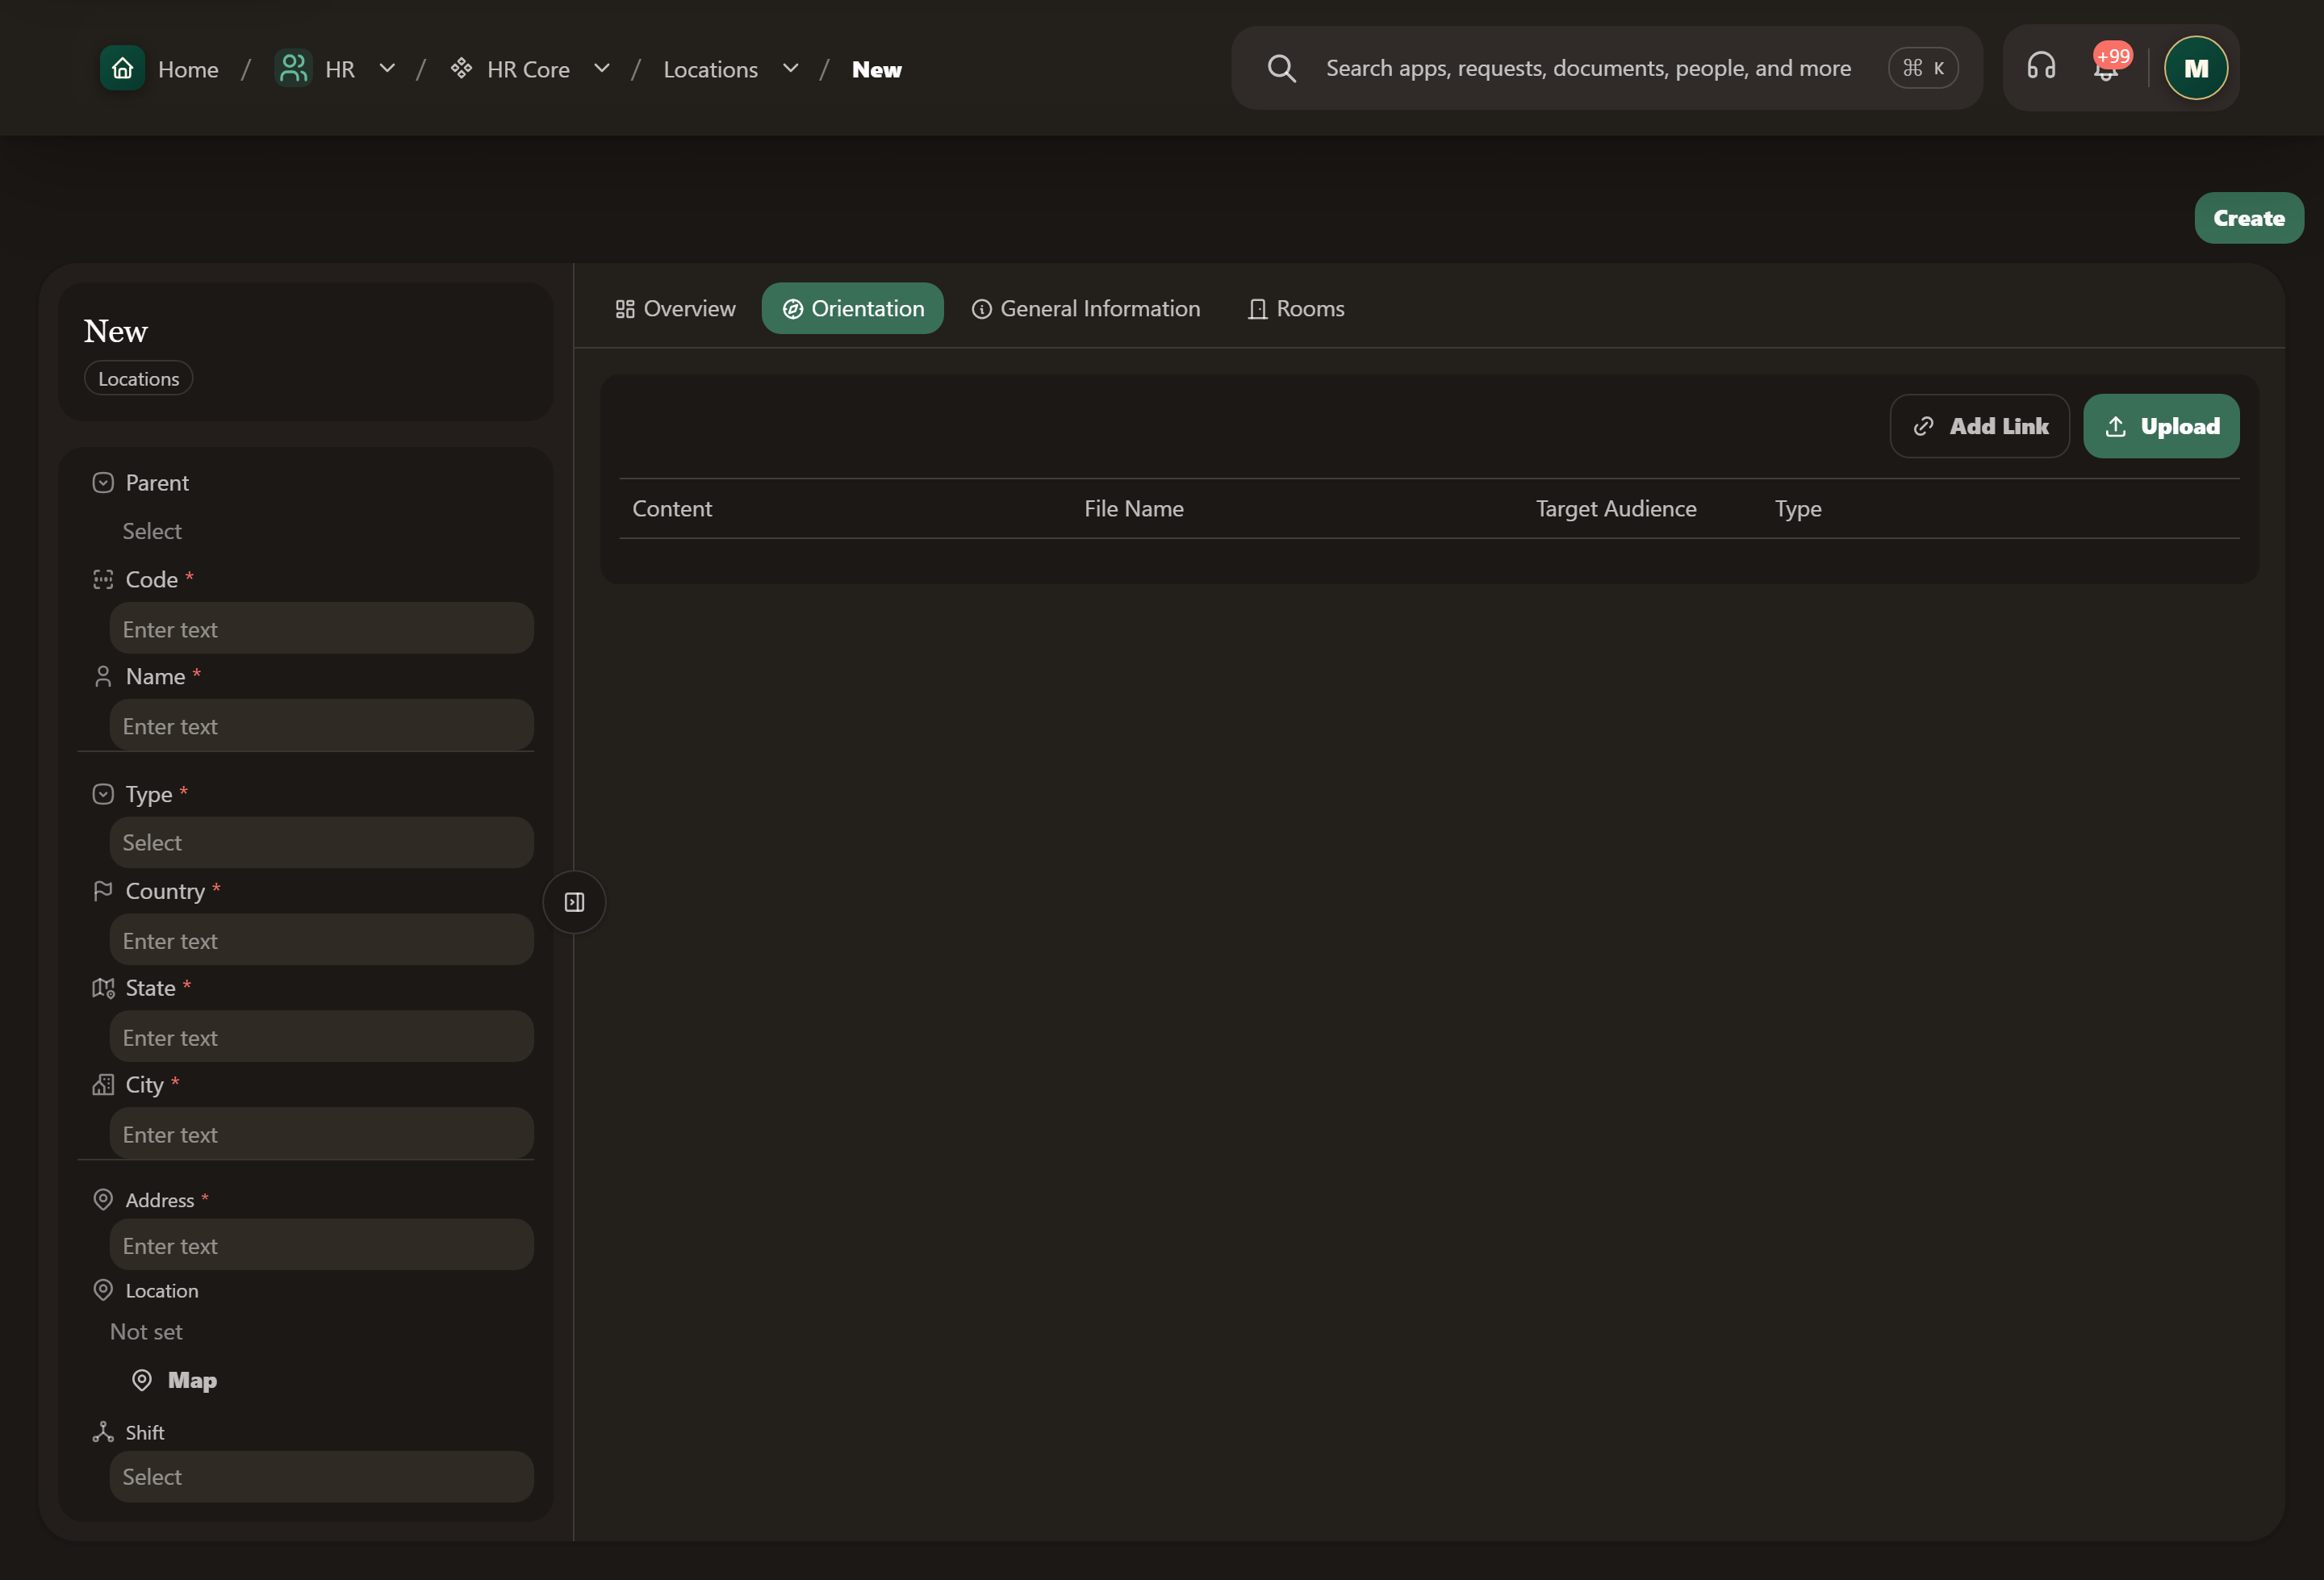
\includegraphics[width=0.95\linewidth]{figures/screens/ch02-location-fields-tab2-en.png}
\caption{Orientation tab in full; unsaved form}
\label{fig:hr-locations-fulltab1}
\end{figure}

\begin{figure}[H]
\centering
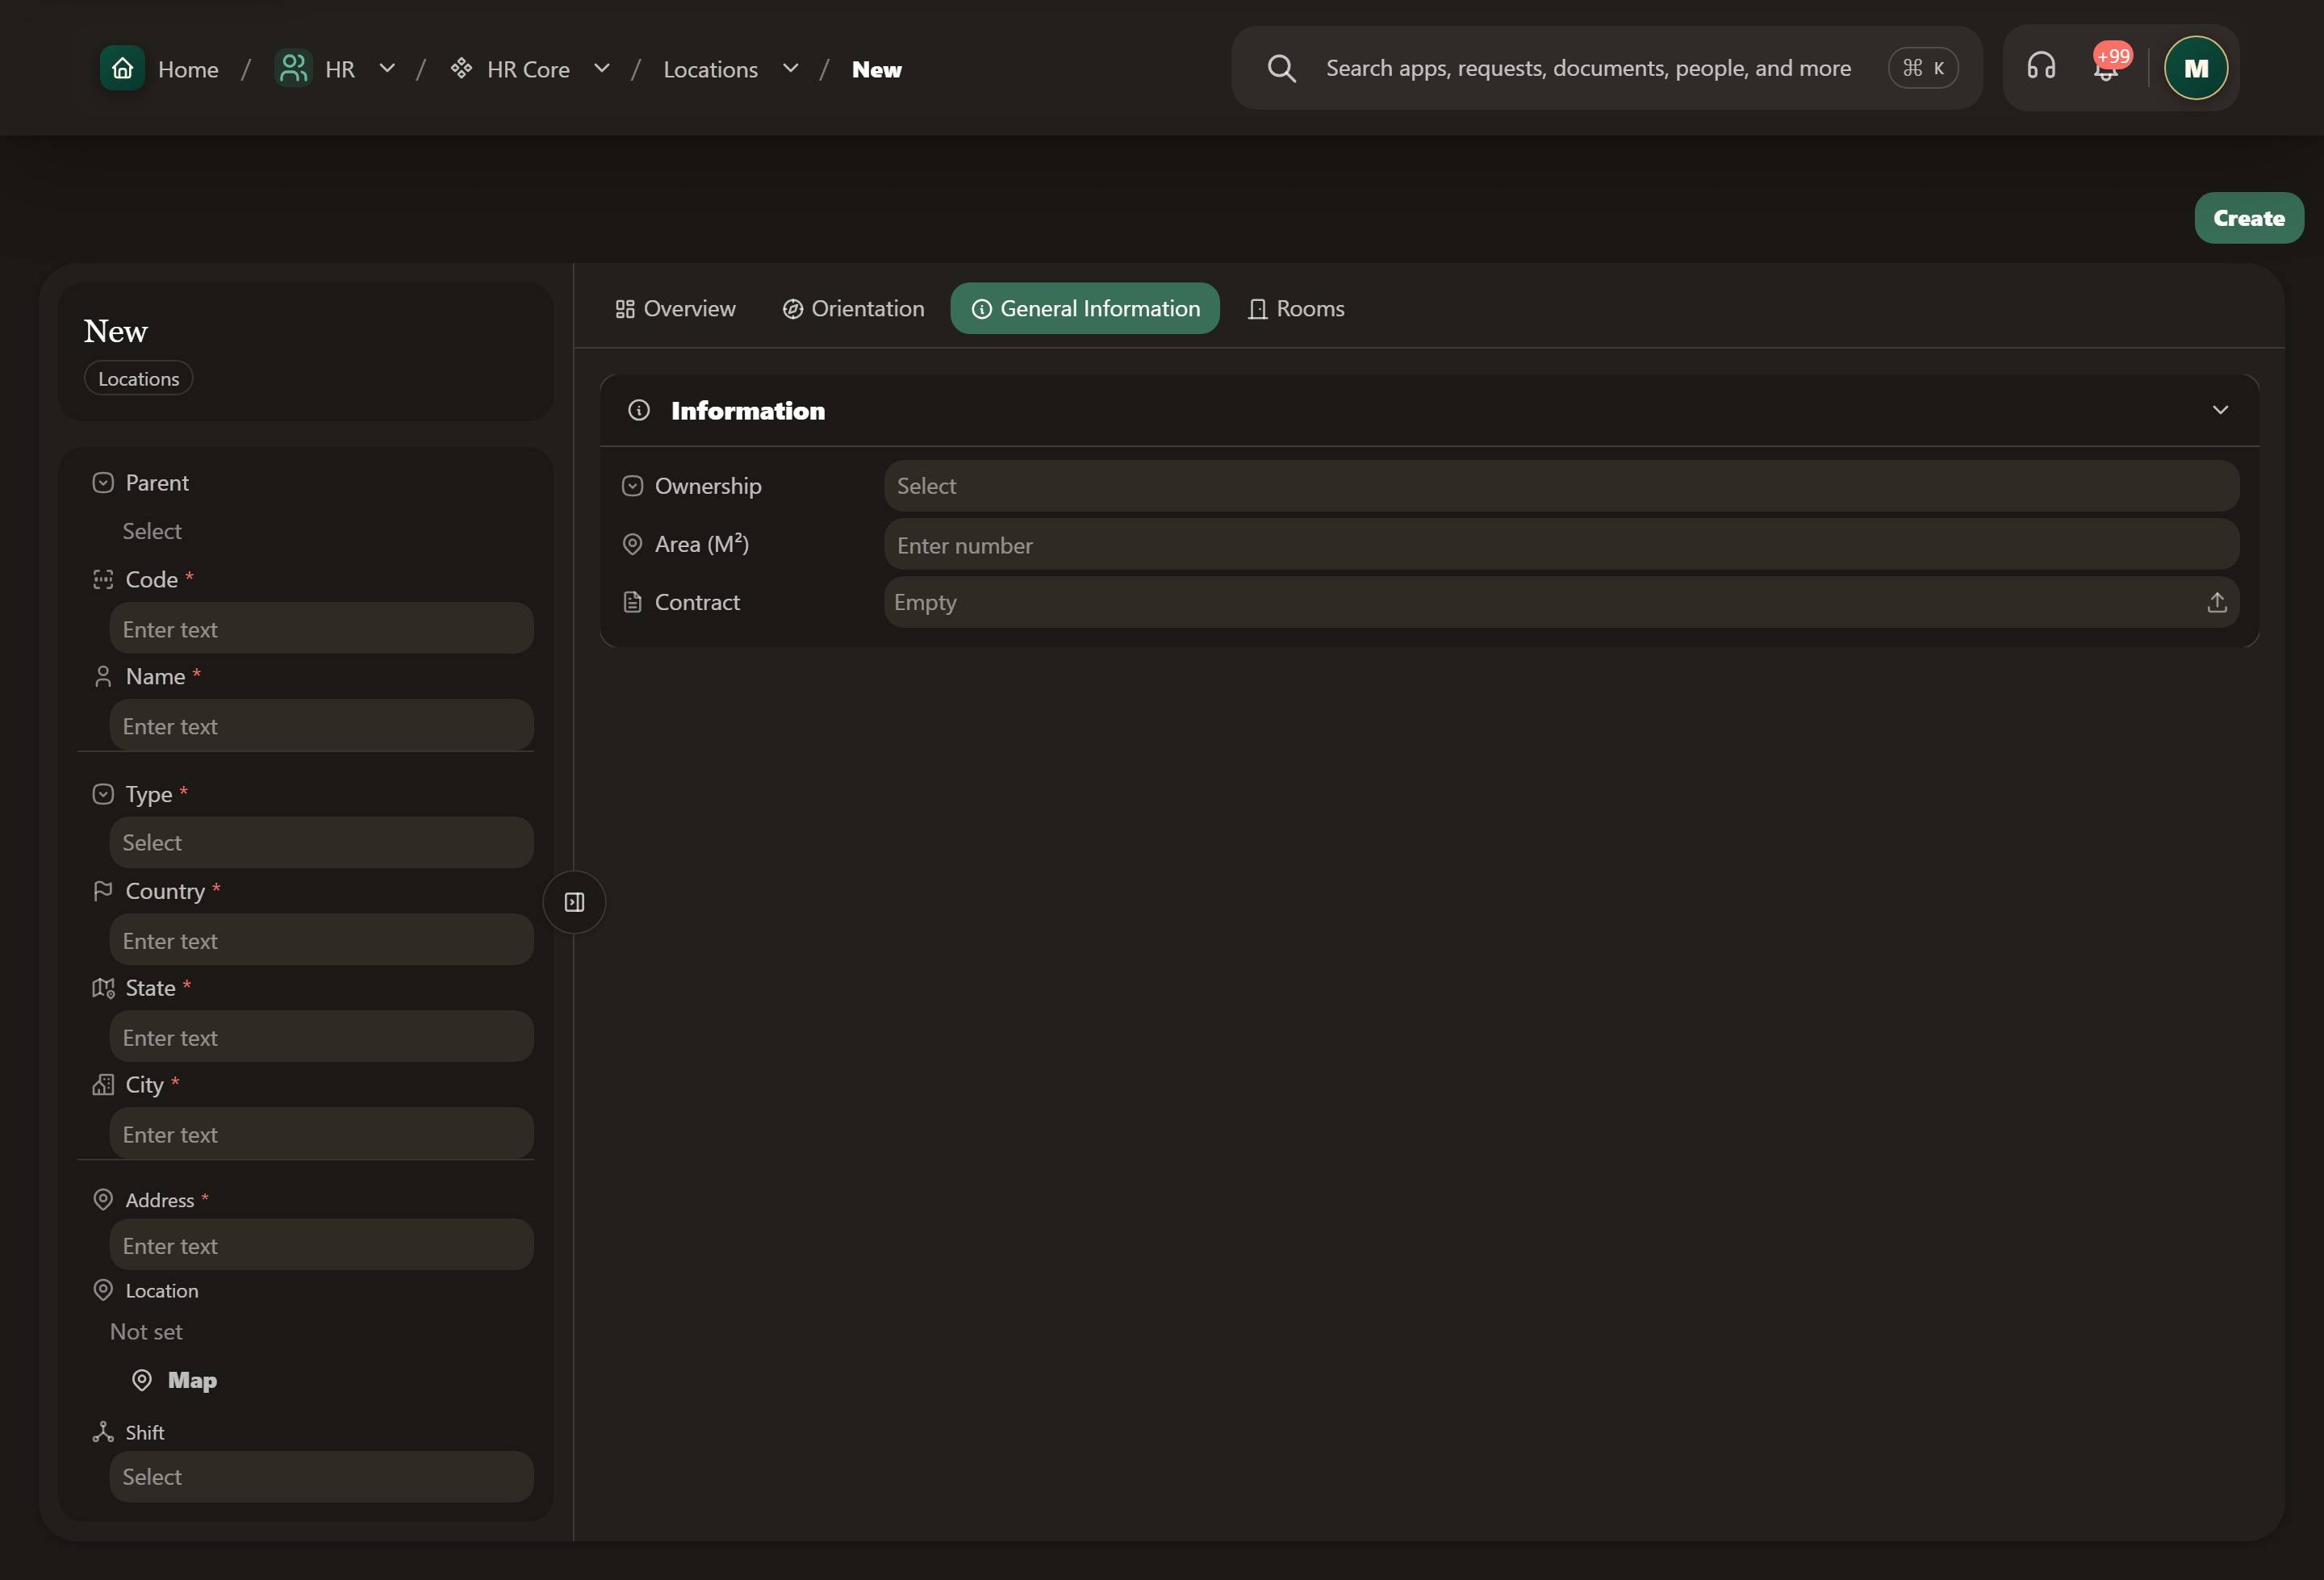
\includegraphics[width=0.95\linewidth]{figures/screens/ch02-location-fields-tab3-en.png}
\caption{General Information tab in full; unsaved form}
\label{fig:hr-locations-fulltab2}
\end{figure}

\begin{figure}[H]
\centering
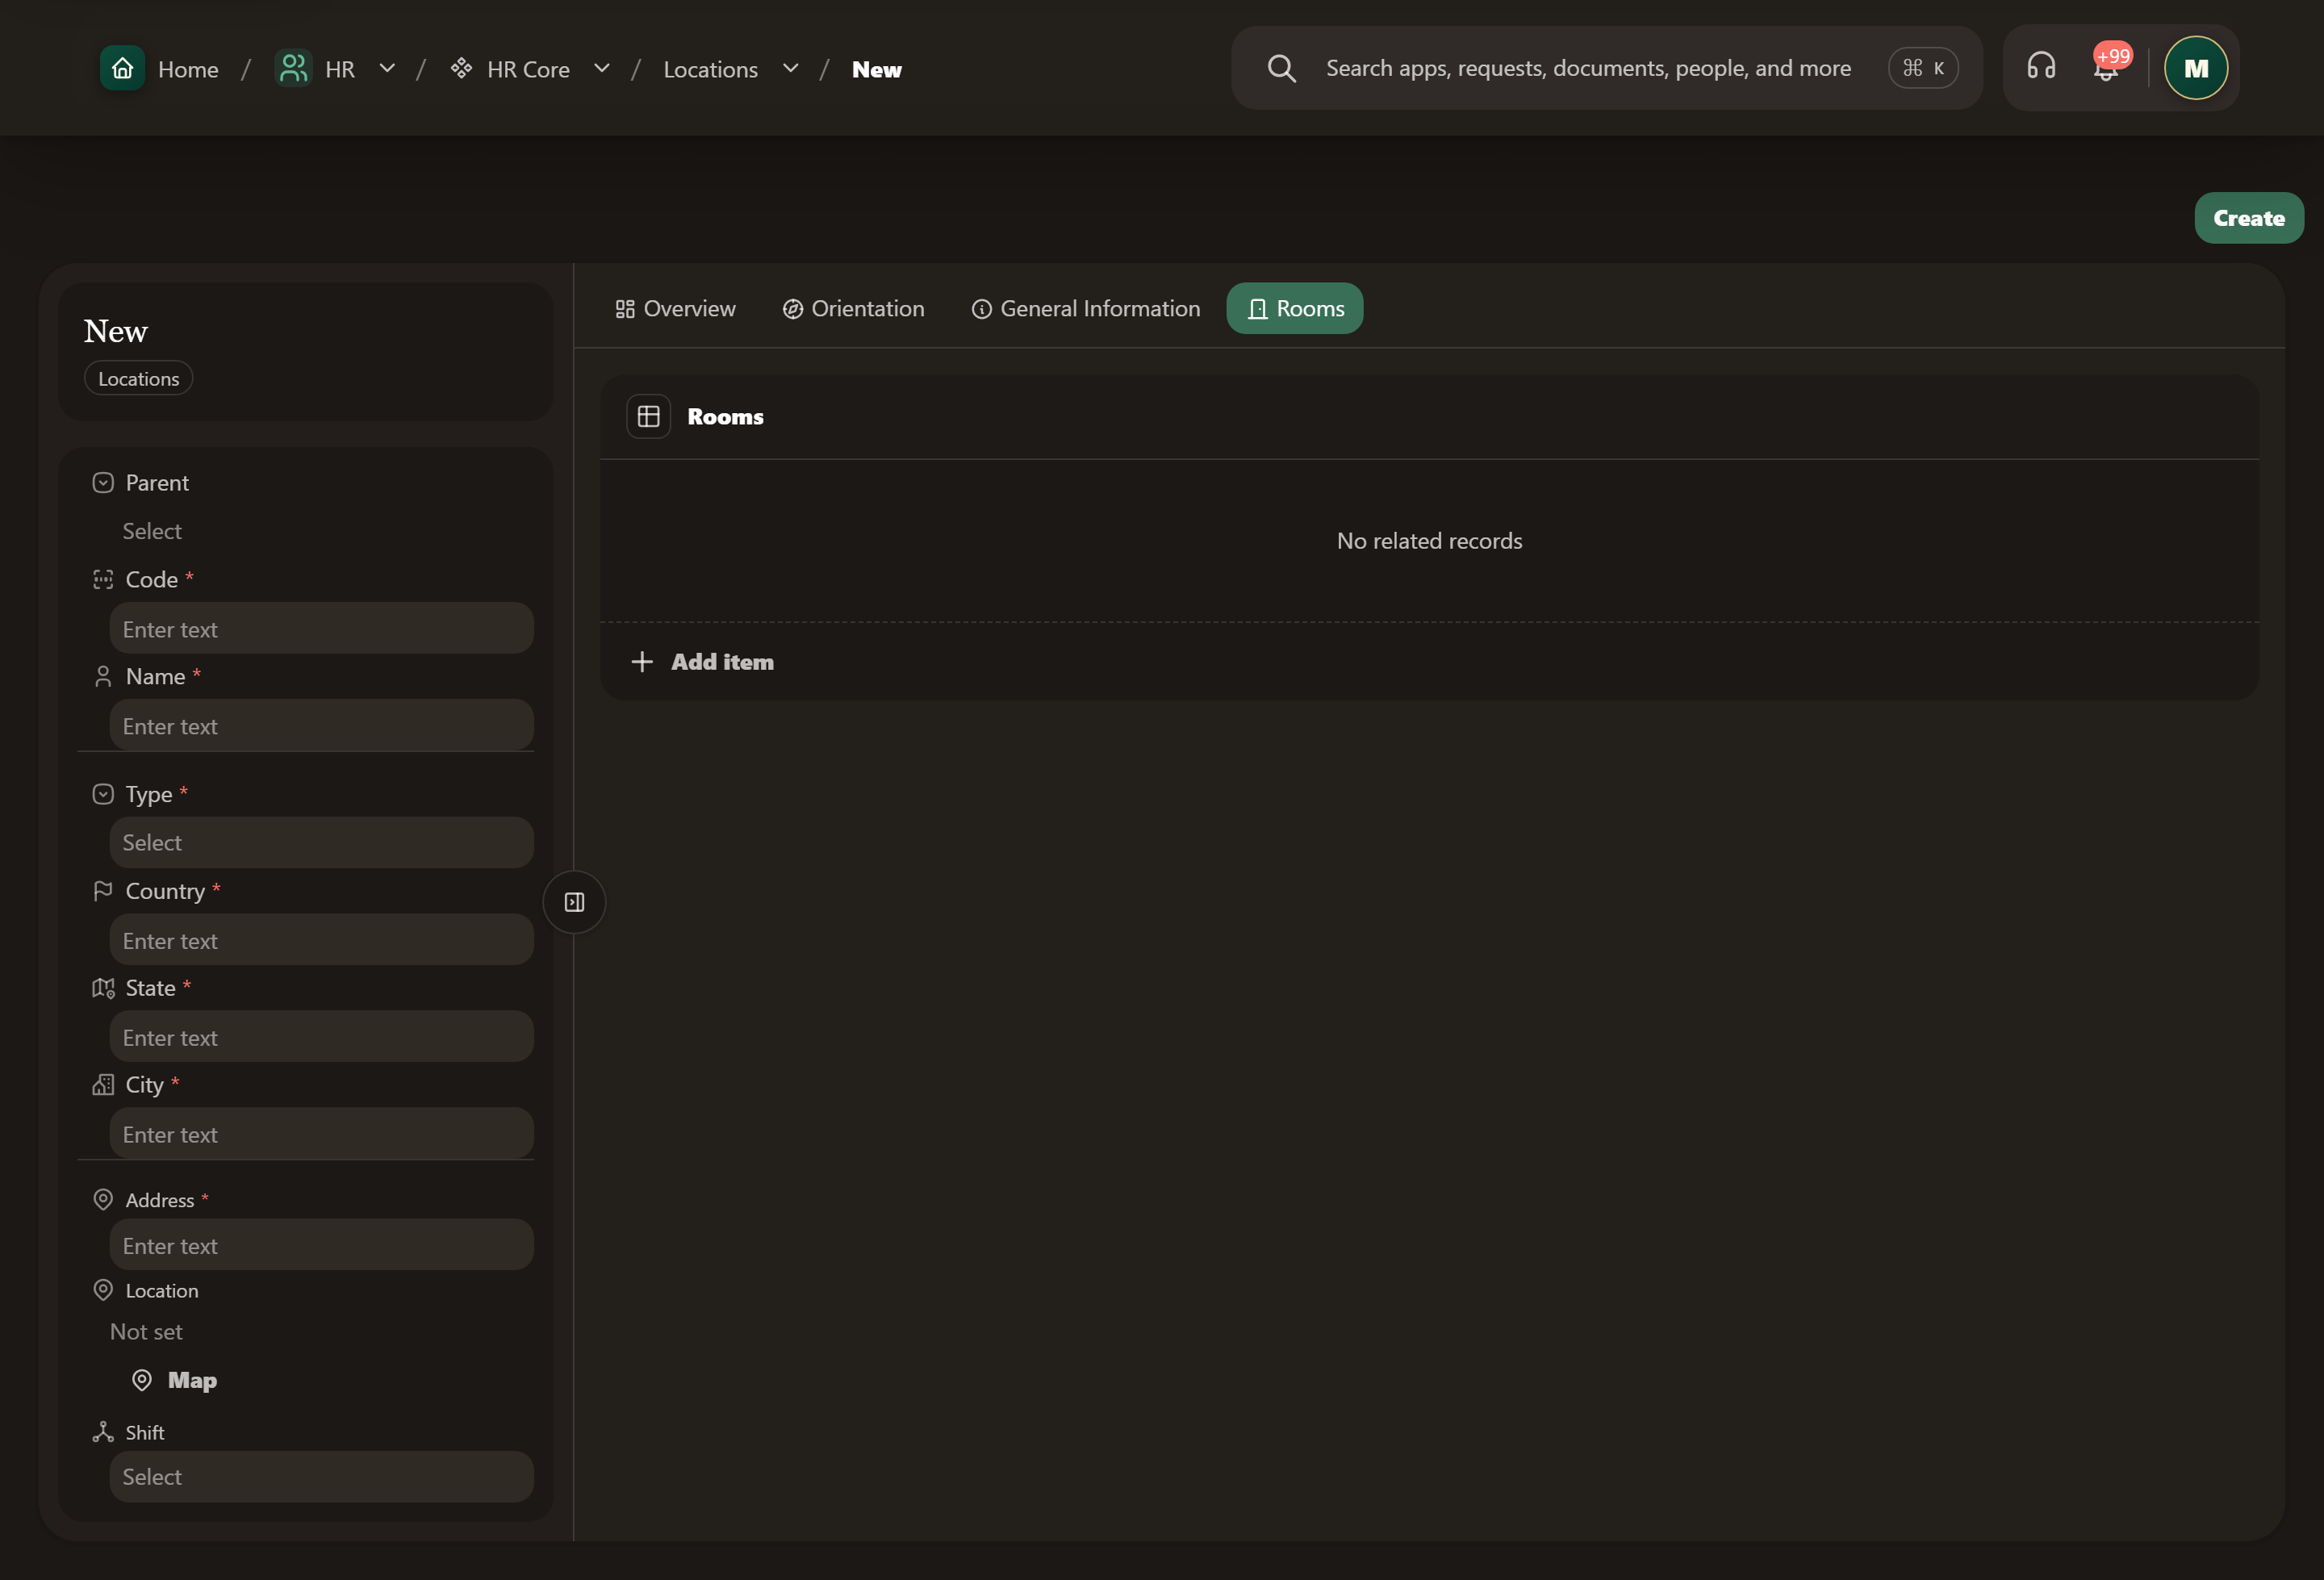
\includegraphics[width=0.95\linewidth]{figures/screens/ch02-location-fields-tab4-en.png}
\caption{Rooms tab in full; unsaved form}
\label{fig:hr-locations-fulltab3}
\end{figure}

\clearpage
\section{Groups}
\label{sec:hr-feature-groups}

A group is a team or committee with members from different units, without changing their jobs.

\textbf{When is it useful?} For example, Horizon's office setup team, or a committee of everyone at the Aleppo Branch. \textbf{Open:} HR / Workforce / Groups.

\begin{figure}[H]
\centering
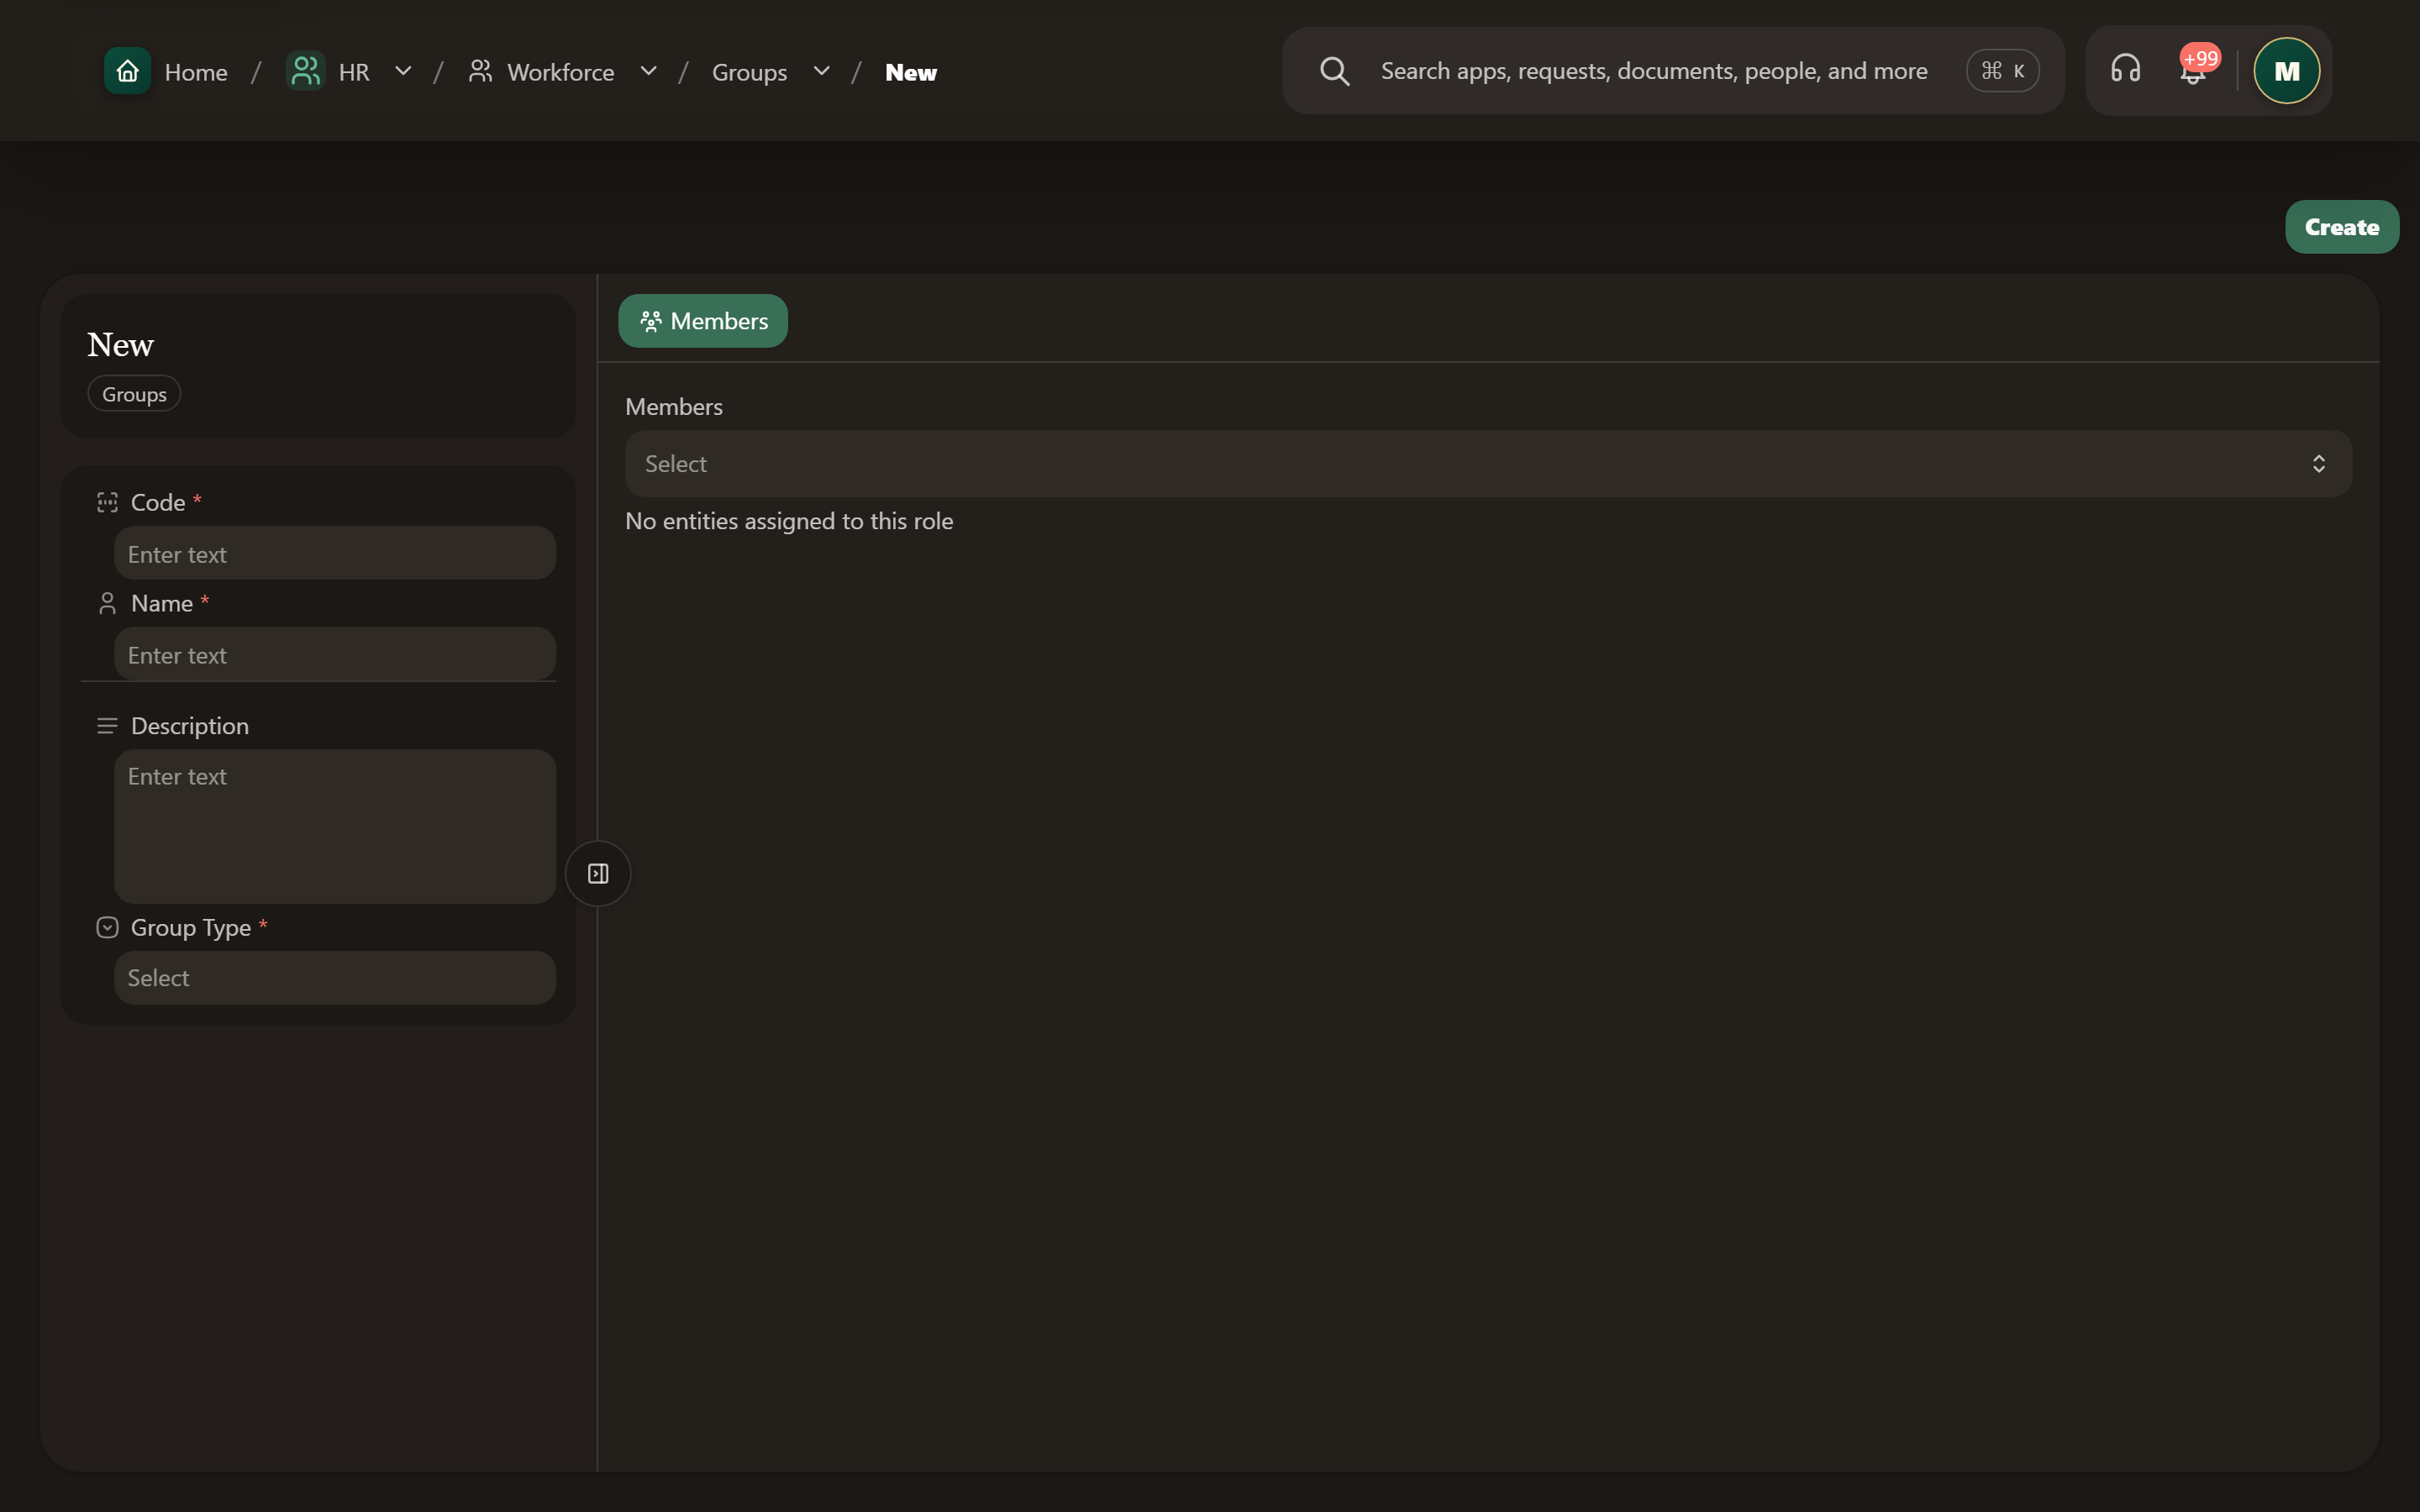
\includegraphics[width=0.95\linewidth]{figures/screens/ch03-feature-groups-en.png}
\caption{Groups: Unsaved form in the test environment}
\label{fig:hr-feature-groups-screen}
\end{figure}

\begin{table}[H]
\centering
\caption{What do you record in a group?}
\label{tab:hr-feature-groups-data}
\rcZebra
\begin{tabularx}{\linewidth}{R{3.6cm} Y}
\rcHeaderRow
\thh{Tab or field} & \thh{What do you add?}\\
Main & Code and Name \req{}, and Description.\\
Group Type & \req{}: “Manual”, where you choose members, or “Code Based”, where a condition selects members and the system counts them \gen{}.\\
Members & People, or everyone in a unit, location, position or group, or the whole organization.\\
Email Accounts & A shared mailbox or a mailing list for the group.\\
\end{tabularx}
\end{table}

\begin{figure}[H]
\centering
\begin{tikzpicture}[node distance=0.5cm,stepBox/.append style={minimum width=6.5cm,text width=6.1cm,minimum height=0.8cm}]
  \node[stepBox] (a) {Define the team};
  \node[stepBox,below=of a] (b) {Choose membership};
  \node[stepBox,below=of b] (c) {Review members};
  \draw[flowsTo] (a) -- (b);
  \draw[flowsTo] (b) -- (c);
\end{tikzpicture}
\rclegend
\caption{Steps of use; arrows do not mean automatic processing}
\label{fig:hr-feature-groups-flow}
\end{figure}

\subsection{Try it and check}

\begin{enumerate}
  \item Open Groups and check that the team does not exist.
  \item Add a code and name, choose “Manual”, then open “Members”, choose Sarah and Omar, and save.
\end{enumerate}

\textbf{Check:} reopen the group and review its members. Joining a group does not change Sarah's assignment as HR Manager.

\begin{figure}[H]
\centering
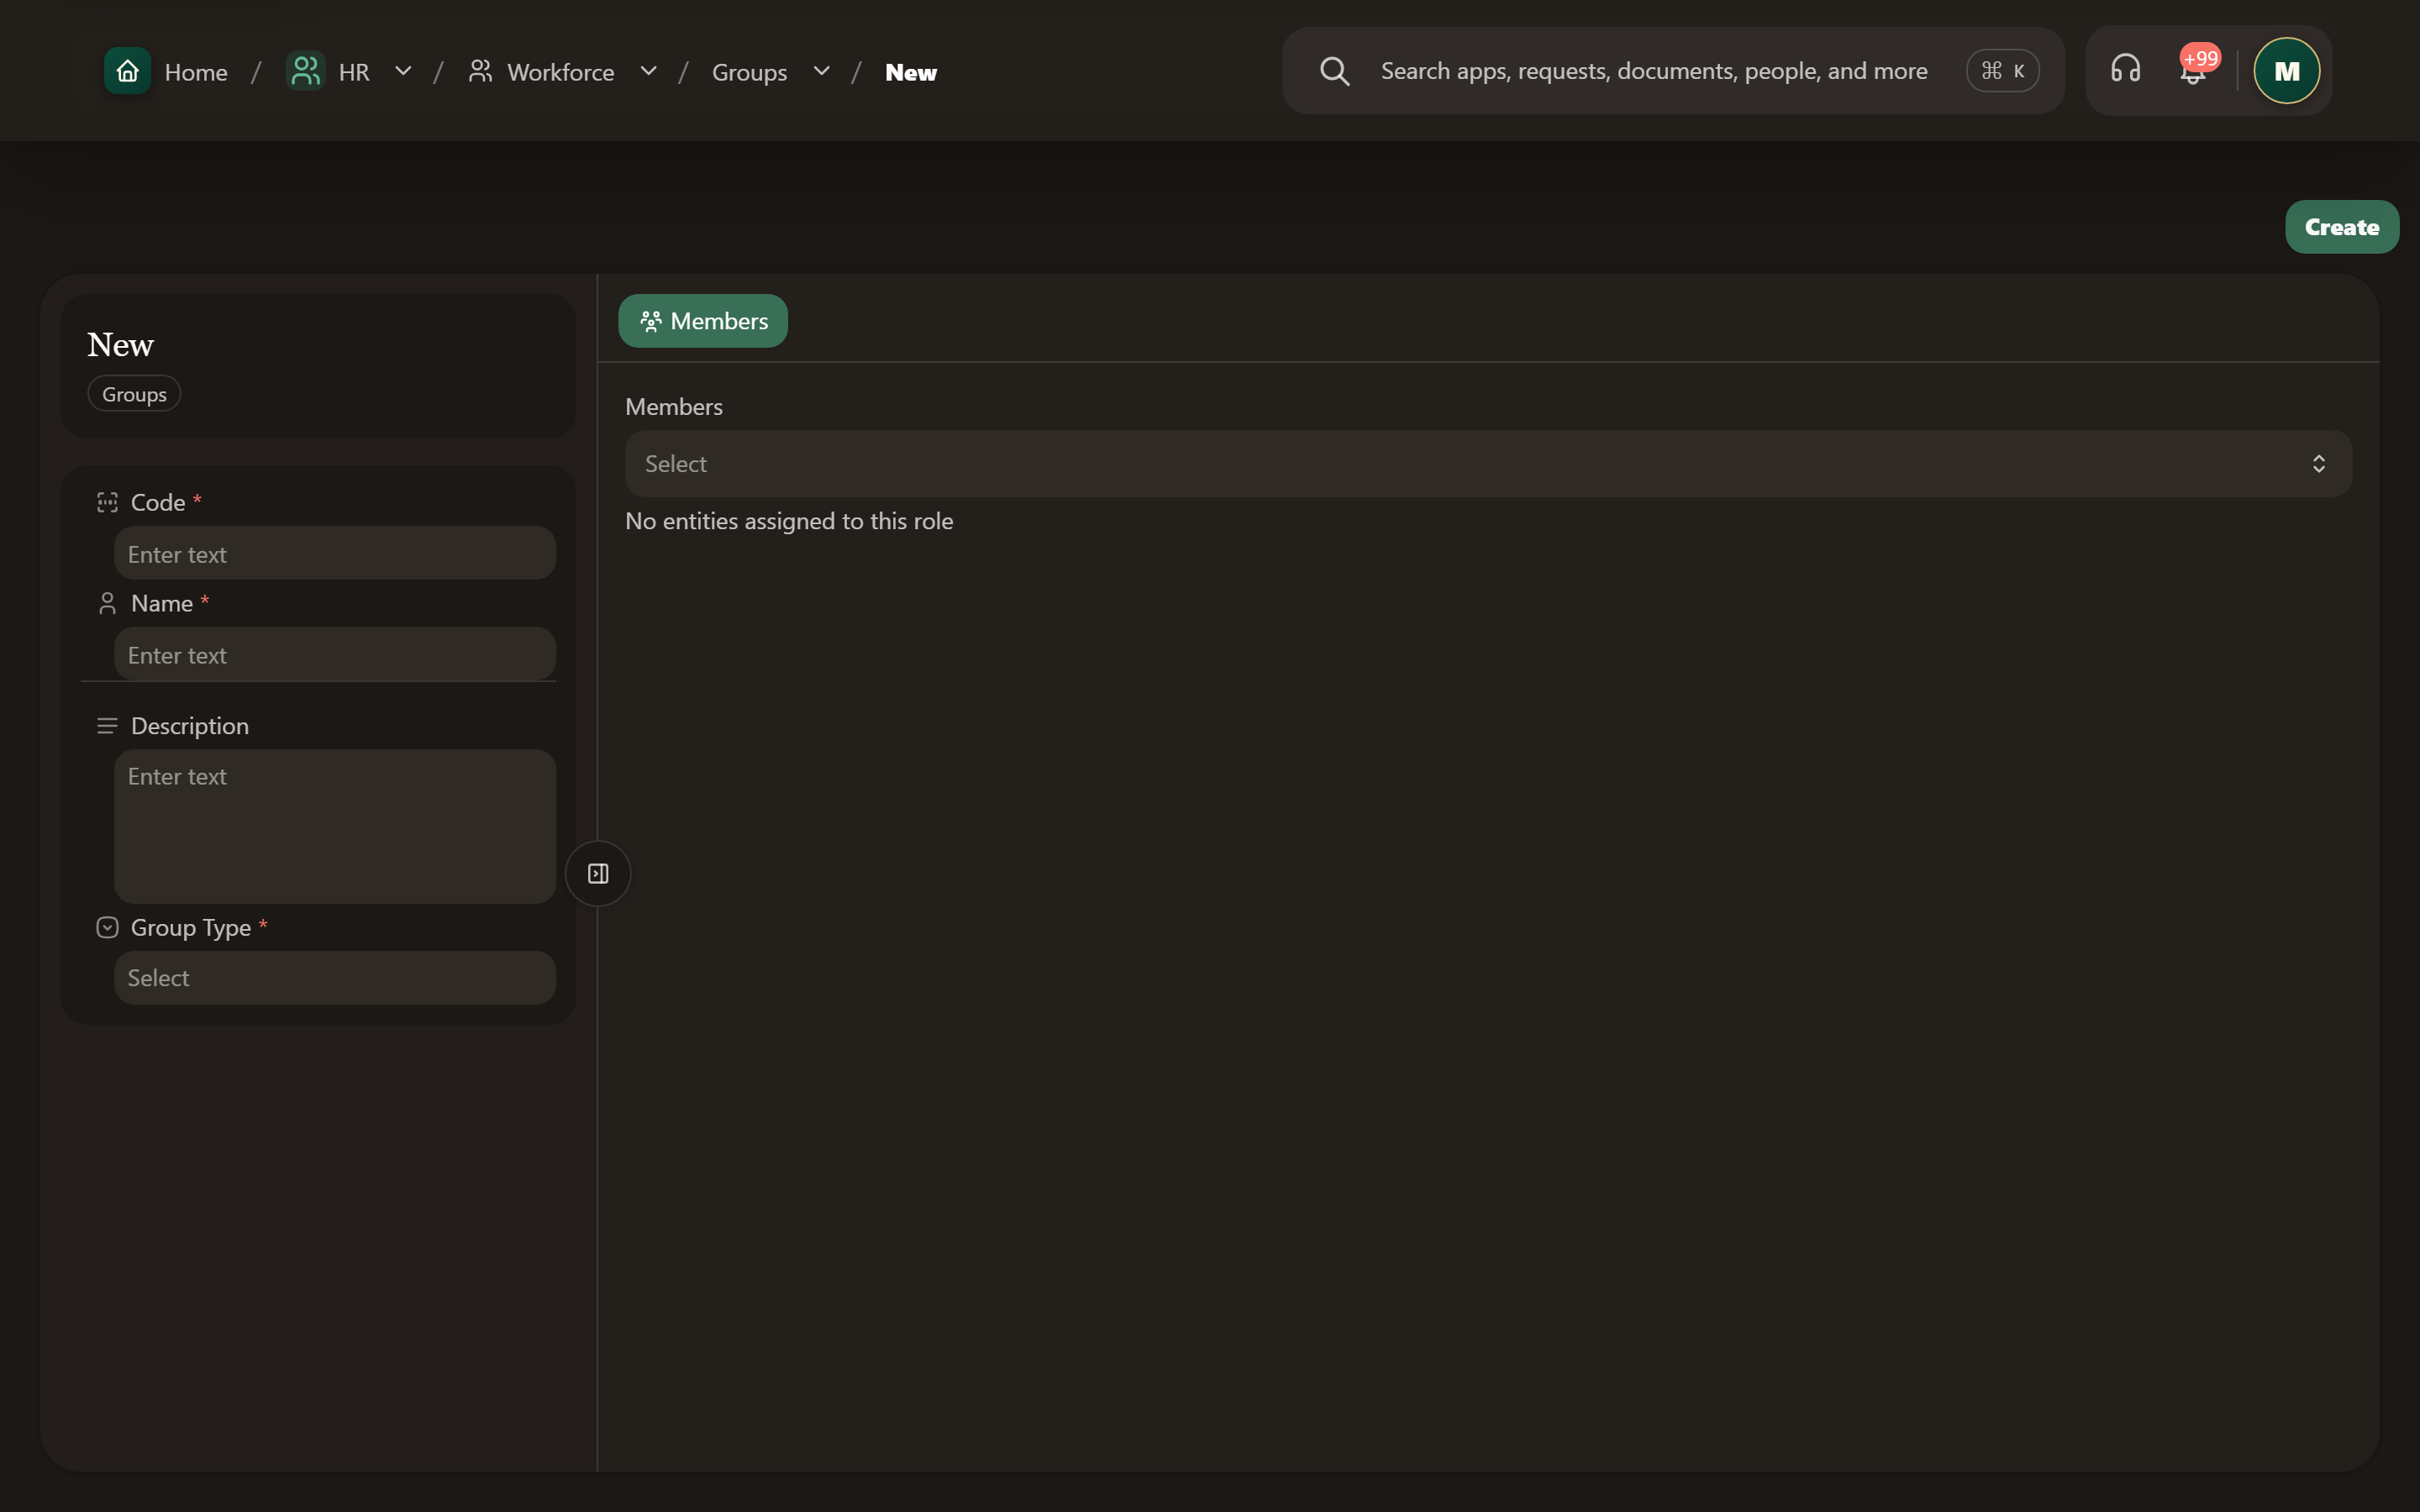
\includegraphics[width=0.95\linewidth]{figures/screens/ch03-feature-groups-tab1-en.png}
\caption{Members tab in full; unsaved form}
\label{fig:hr-groups-fulltab1}
\end{figure}

\clearpage
\section{Shifts}
\label{sec:hr-feature-shifts}

A shift sets the expected working days, hours and breaks. Attendance records what actually happened.

\textbf{When is it useful?} One schedule for everyone with the same pattern, instead of repeating times for each employee. \textbf{Open:} HR / Time / Shifts.

\begin{figure}[H]
\centering
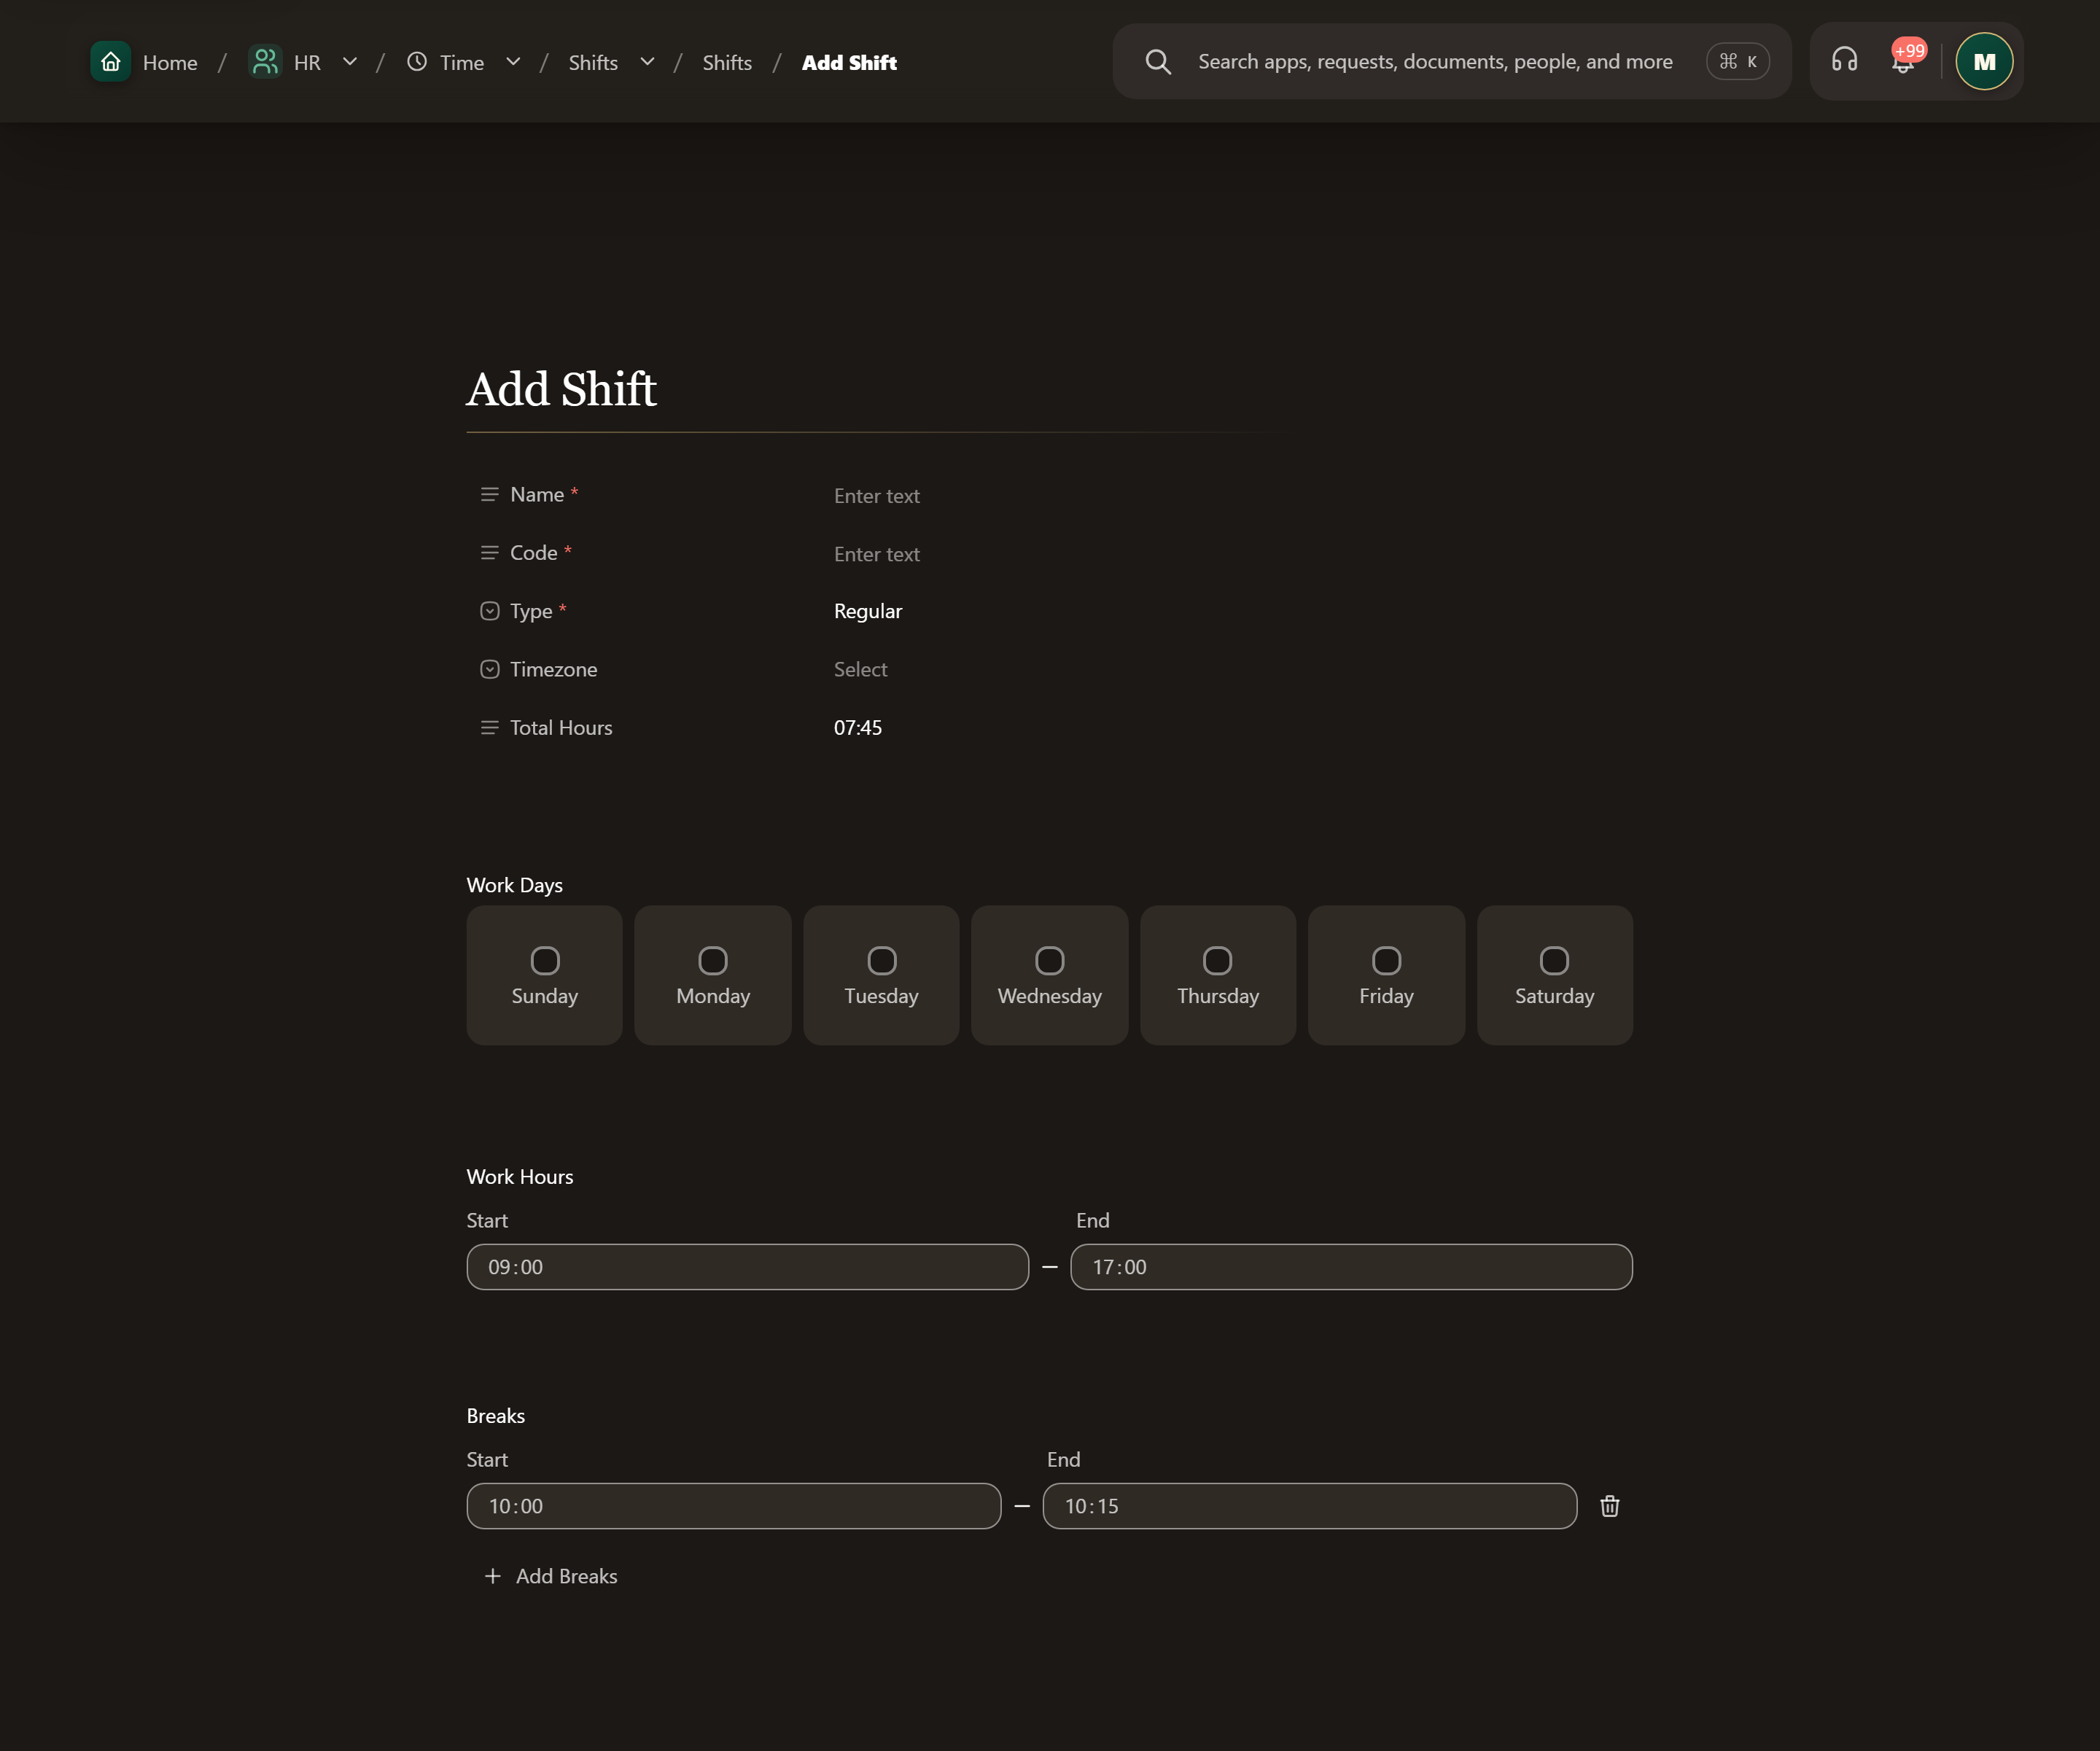
\includegraphics[width=0.95\linewidth]{figures/screens/ch03-shift-example-en.png}
\caption{Shifts: full add form; not saved}
\label{fig:hr-feature-shifts-screen}
\end{figure}

\begin{table}[H]
\centering
\caption{Choosing the shift type}
\label{tab:hr-shift-types}
\rcZebra
\begin{tabularx}{\linewidth}{R{2.4cm} Y Y}
\rcHeaderRow
\thh{Type} & \thh{What do you enter?} & \thh{Example}\\
Regular & One work period, with breaks when needed. & From 09:00 to 17:00.\\
Split & More than one work period, without overlap. & From 09:00 to 13:00, then from 16:00 to 20:00.\\
Flexible & The work duration in hours and minutes. & A duration of 08:00, with no start or end.\\
Marathon & The work duration in hours and minutes. & The guide does not assume a work–rest cycle from the name alone.\\
\end{tabularx}
\end{table}

\begin{table}[H]
\centering
\caption{What do you record in a shift?}
\label{tab:hr-feature-shifts-data}
\rcZebra
\begin{tabularx}{\linewidth}{R{3.6cm} Y}
\rcHeaderRow
\thh{Field} & \thh{What do you add?}\\
Name, Code and Type & \req{}; the code must be unique.\\
Work Days & \req{}: at least one day from Sunday to Saturday.\\
Timezone & Such as Asia/Damascus \opt{}.\\
Work Hours and Breaks & For Regular and Split; a break stays inside working time \opt{}.\\
Duration & For Flexible and Marathon; it cannot be 00:00.\\
Total Hours & Work hours minus breaks \gen{}.\\
\end{tabularx}
\end{table}

\subsection{Create the shift step by step}
\label{sec:hr-shifts}

\begin{enumerate}
  \item Open Shifts and add “Office Hours”, code HZN-S-01, type “Regular”.
  \item Choose Sunday to Thursday and Asia/Damascus.
  \item Work Hours: 09:00–17:00. Edit the existing break to 13:00–13:30; do not add a second one.
  \item Check Total Hours = 07:30, then “Save”. Reopen the shift and check the values.
\end{enumerate}

\begin{rcnote}[Avoid time errors]
Periods must not overlap; breaks stay inside working time. 22:00–06:00 ends the next day. Equal start and end is not allowed.
\end{rcnote}

\subsection{How the shift reaches the employee}
\label{sec:hr-shift-inheritance}

Inheritance: the employee uses the shift of a higher record instead of repeating it.

\begin{figure}[H]
\centering
\begin{tikzpicture}[node distance=0.4cm,stepBox/.append style={minimum width=6.5cm,text width=6.1cm,minimum height=0.7cm}]
  \node[stepBox] (a) {Assignment shift};
  \node[stepBox,below=of a] (p) {Position shift};
  \node[stepBox,below=of p] (n) {Unit shift, then its\\parent units};
  \node[stepBox,below=of n] (l) {Location shift, then\\its parent locations};
  \draw[flowsTo] (a) -- (p);
  \draw[flowsTo] (p) -- (n);
  \draw[flowsTo] (n) -- (l);
\end{tikzpicture}
\rclegend
\caption{Order of the shift search: move to the next level only if no shift is found}
\label{fig:hr-shift-order}
\end{figure}

Stop at the first shift found; shifts are not combined.

\begin{enumerate}
  \item Open Nodes / HZN-HR. Choose “Office Hours” in “Shift”; if needed choose “Override” first, then save.
  \item Open Positions / HR Manager and check the unit and shift.
  \item Open Sarah's assignment and check the shift. If it differs, check the assignment, then the position, as in the diagram.
\end{enumerate}

\textbf{Check:} the right shift appears in Sarah's assignment. “Reset” restores inheritance. Shift does not save? Check name, code, days and overlapping periods. Duration lower than expected? Breaks are subtracted. Cannot delete? It is used by assignments, positions or attendance.

\clearpage
\section{My attendance}
\label{sec:hr-feature-my-attendance}

My attendance shows your calculated month: working days and holidays, and for each day the punches, totals and their effect on pay.

\textbf{When is it useful?} Understand your day before requesting a correction. An empty day calls for checking the source; it does not prove absence. \textbf{Open:} HR / Time / My attendance.

\begin{figure}[H]
\centering
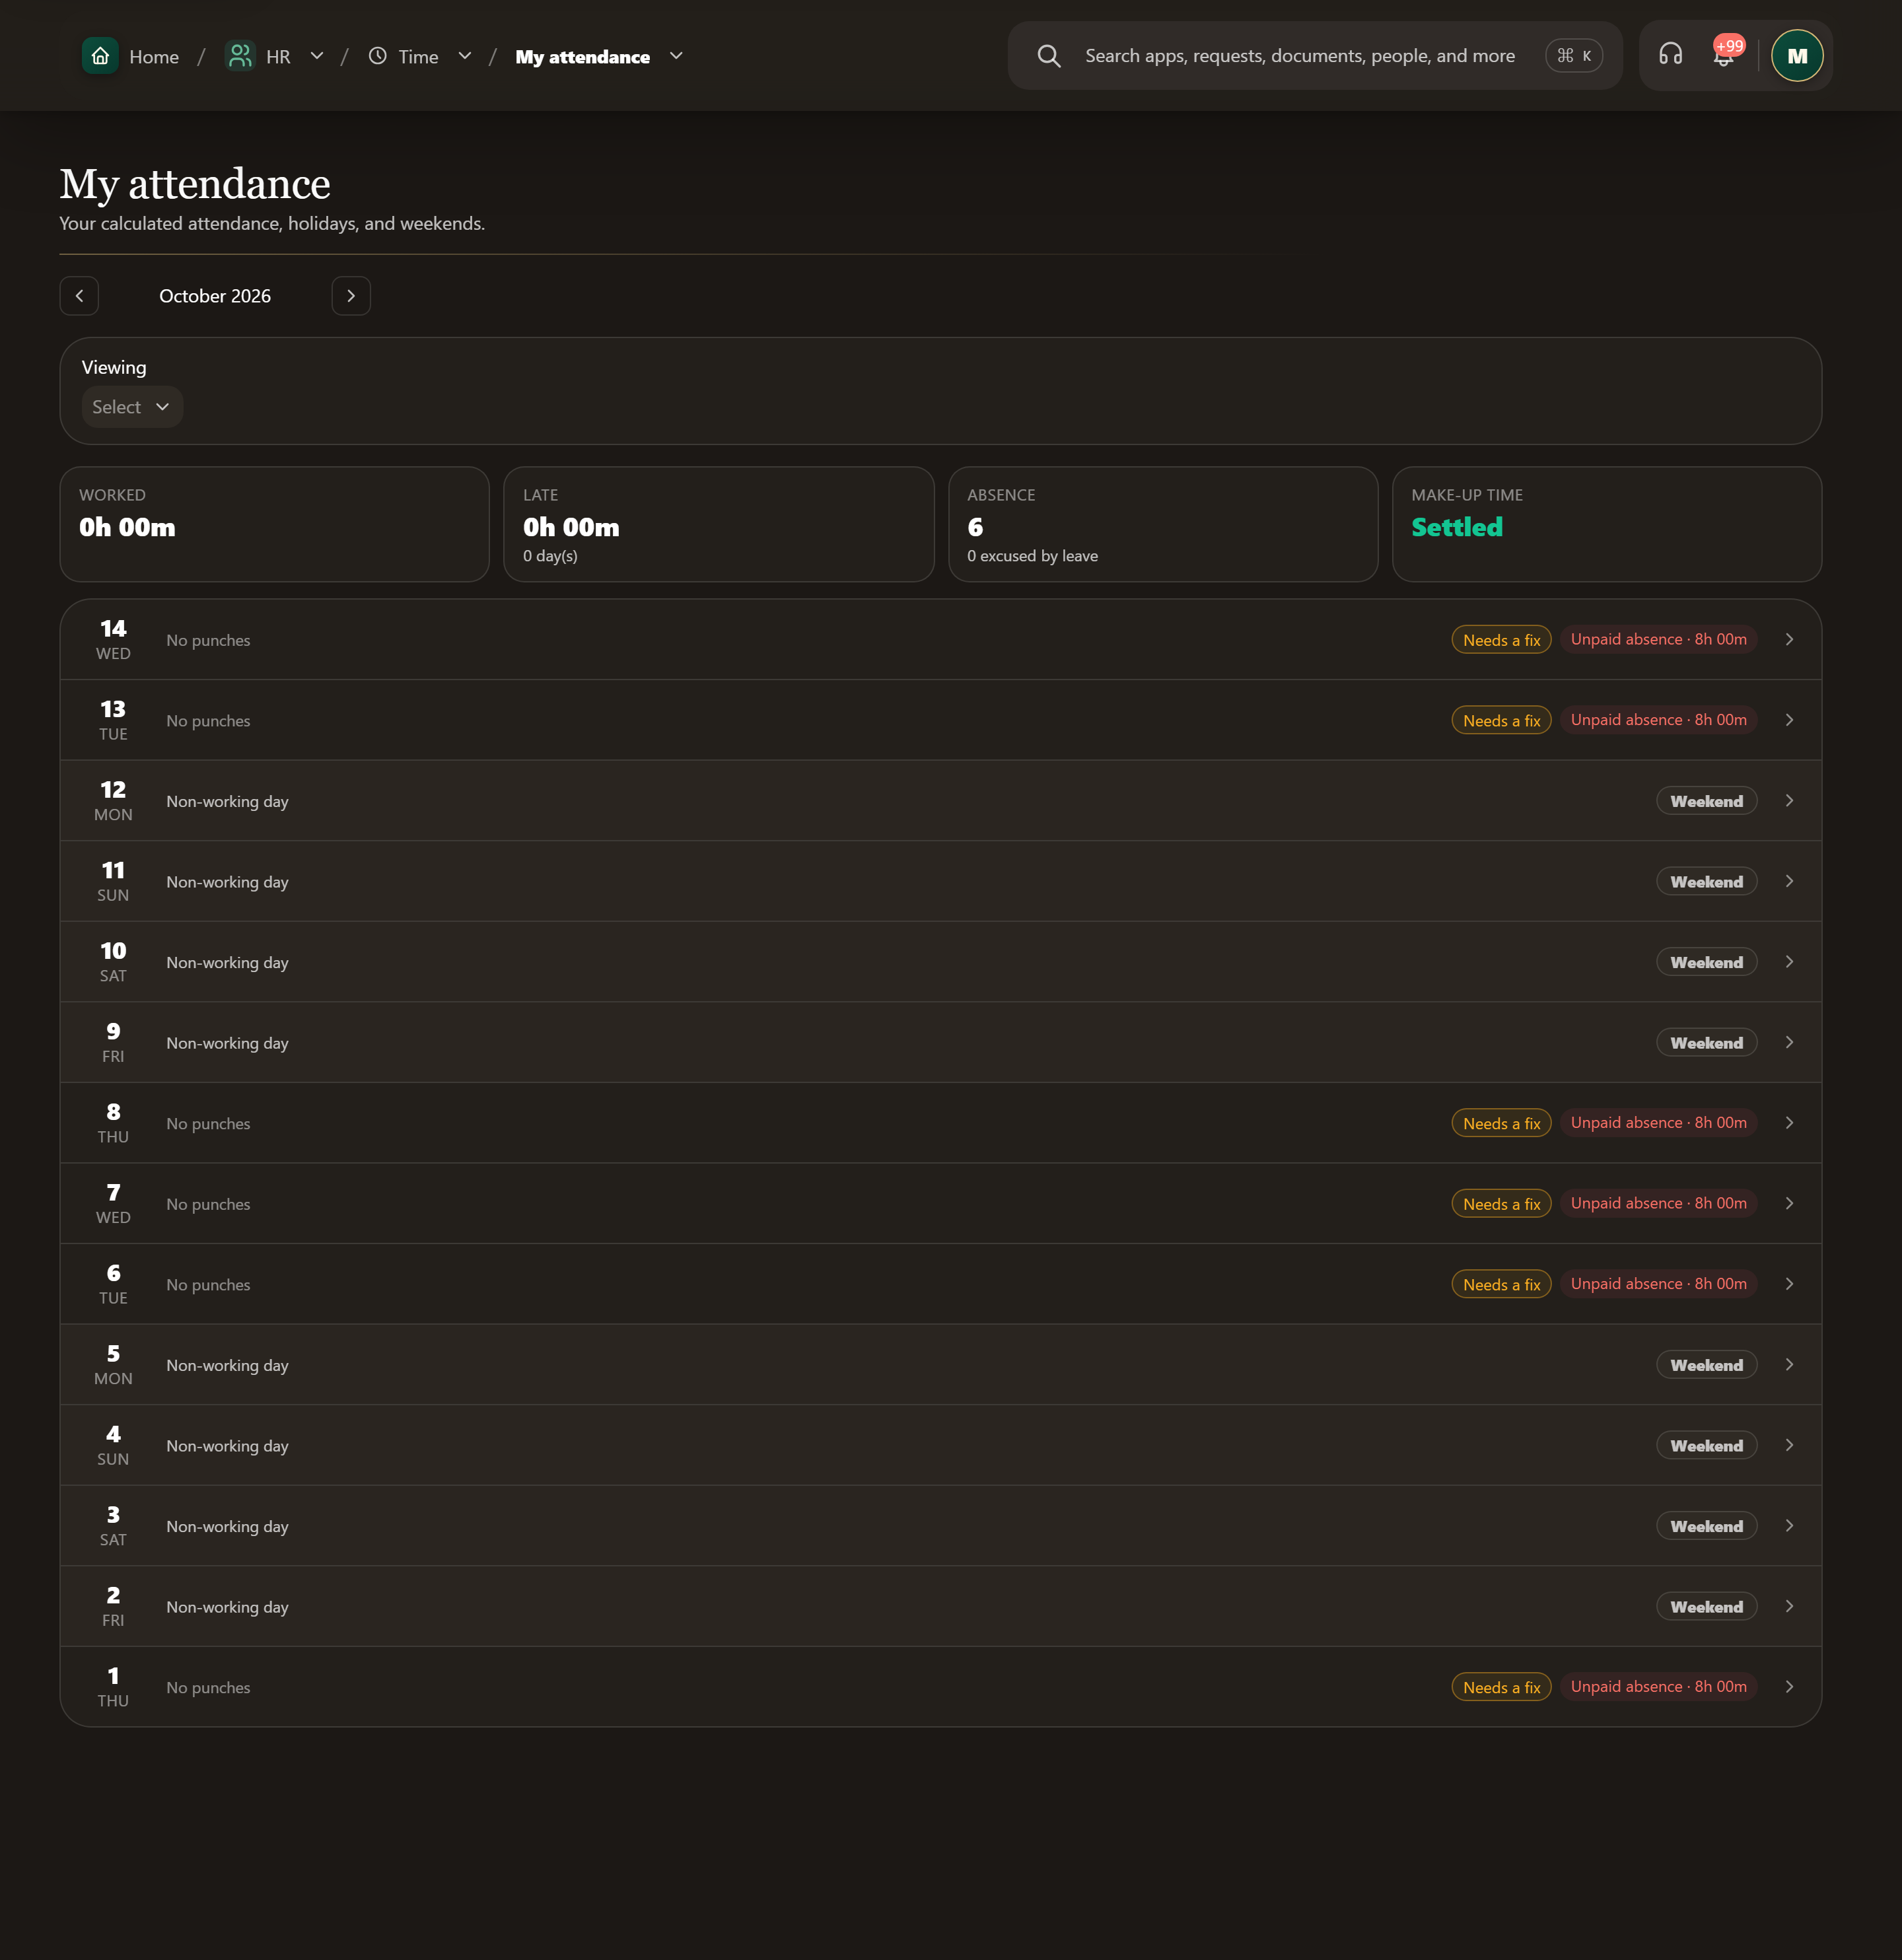
\includegraphics[width=0.95\linewidth]{figures/screens/ch03-feature-my-attendance-en.png}
\caption{My attendance: English interface in the test environment}
\label{fig:hr-feature-my-attendance-screen}
\end{figure}

\begin{table}[H]
\centering
\caption{What do you see in My attendance?}
\label{tab:hr-feature-my-attendance-data}
\rcZebra
\begin{tabularx}{\linewidth}{R{3.6cm} Y}
\rcHeaderRow
\thh{Part} & \thh{What does it show?}\\
Month summary & Worked, Late and its days, Absence and how much leave excused, Make-up time.\\
Days of the month & For each day: Normal, Holiday, Weekend, No punches, Needs a fix, Locked.\\
Day page & Shift and policy, the punch timeline, “Totals for the day”, “On the slip”, “How this was calculated”.\\
\end{tabularx}
\end{table}

\subsection{What can you do?}

\begin{itemize}
  \item Move between months, and from one day to the next.
  \item “Fix this day”: add an In or Out punch and choose a reason: Forgot to punch, Device failure, Duplicated scan, Wrong direction read, Off-site work, or Other with a justification.
  \item “Send for review”, and “Withdraw” while the request is pending.
  \item View another member's attendance with permission; the correction remains theirs to request.
\end{itemize}

\begin{figure}[H]
\centering
\begin{tikzpicture}[node distance=0.4cm,stepBox/.append style={minimum width=6cm,text width=5.6cm,minimum height=0.7cm}]
  \node[stepBox] (s0) {My attendance: month\\and day};
  \node[stepBox,below=of s0] (s1) {Compare shift and\\clocking times};
  \node[stepBox,below=of s1] (s2) {Check any leave or\\holiday};
  \node[stepBox,below=of s2] (s3) {Check correction and\\decision};
  \draw[flowsTo] (s0) -- (s1);
  \draw[flowsTo] (s1) -- (s2);
  \draw[flowsTo] (s2) -- (s3);
\end{tikzpicture}
\rclegend
\caption{Review one day}
\label{fig:hr-day-review}
\end{figure}

\subsection{Try it and check}

\begin{enumerate}
  \item Open My attendance, choose the month, then the day.
  \item Compare the shift with clock-in, clock-out and duration, and read “How this was calculated”.
  \item If a punch is missing, choose “Fix this day”, add it with a reason, then “Send for review”.
\end{enumerate}

\textbf{Check:} the day shows that a correction is pending review. The shift sets expected time; the policy decides lateness and overtime; do not assume an automatic deduction. If the fix button is missing, its deadline may have passed.

\clearpage
\section{Timesheets}
\label{sec:hr-feature-timesheets}

Timesheets show the team's attendance for a day, week or month, and let you approve recorded time.

\textbf{When is it useful?} Reviewing the team's week, or preparing time before payroll. \textbf{Open:} HR / Time / Timesheets.

\begin{figure}[H]
\centering
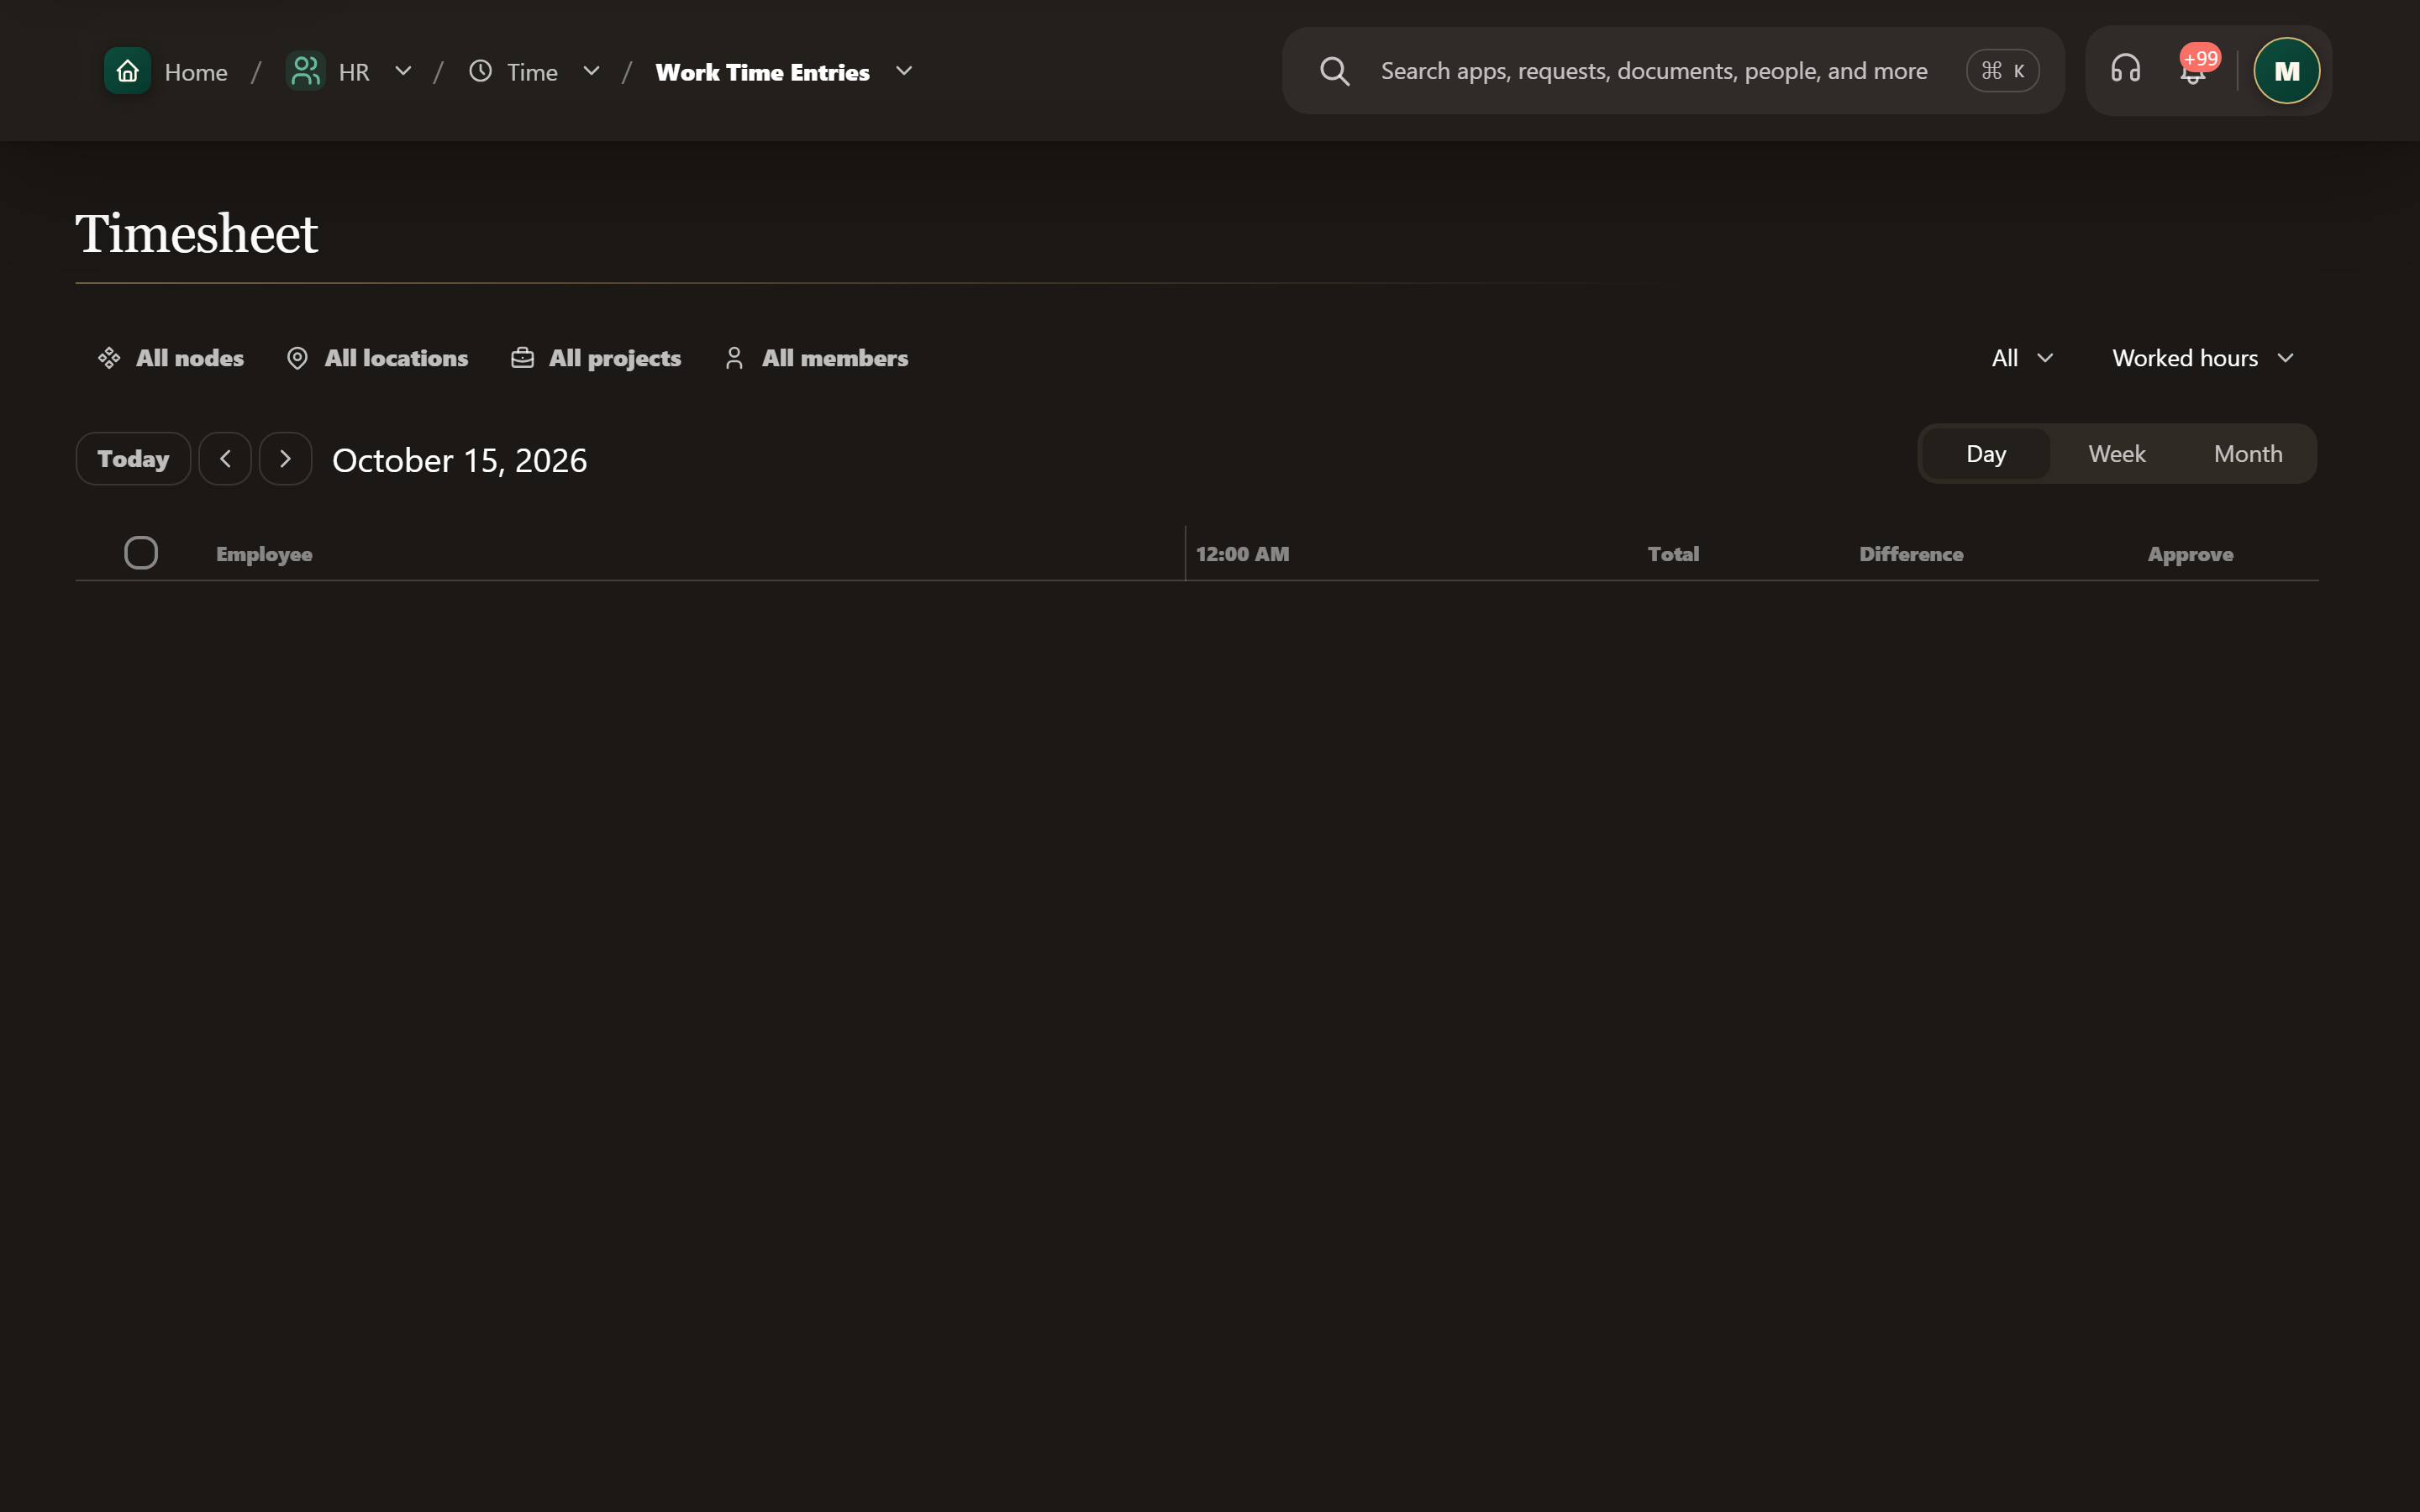
\includegraphics[width=0.95\linewidth]{figures/screens/ch03-feature-timesheets-en.png}
\caption{Timesheets: English interface in the test environment}
\label{fig:hr-feature-timesheets-screen}
\end{figure}

\begin{table}[H]
\centering
\caption{What do you see in Timesheets?}
\label{tab:hr-feature-timesheets-data}
\rcZebra
\begin{tabularx}{\linewidth}{R{3.6cm} Y}
\rcHeaderRow
\thh{Part} & \thh{What does it show?}\\
Filters & Nodes, locations, projects and members, and hours: worked only, with justified leaves, or with paid leaves.\\
Period & “Today”, or Day, Week or Month.\\
Day cell & Entry, break, leave time and total work; or the holiday name.\\
Totals & Avg worktime, Avg delay, Total, Difference.\\
\end{tabularx}
\end{table}

\subsection{What can you do?}

\begin{itemize}
  \item Day view: a timeline per employee with work, breaks and unjustified absence.
  \item “Approve” one row, or select several rows and approve them together; filter approved or not approved.
  \item A discrepancy flag opens Attendance Corrections. There is no add or import on this page.
\end{itemize}

\begin{figure}[H]
\centering
\begin{tikzpicture}[node distance=0.5cm,stepBox/.append style={minimum width=6.5cm,text width=6.1cm,minimum height=0.8cm}]
  \node[stepBox] (a) {Choose people\\and period};
  \node[stepBox,below=of a] (b) {Review days\\and totals};
  \node[stepBox,below=of b] (c) {Check discrepancies};
  \draw[flowsTo] (a) -- (b);
  \draw[flowsTo] (b) -- (c);
\end{tikzpicture}
\rclegend
\caption{Steps of use; arrows do not mean automatic processing}
\label{fig:hr-feature-timesheets-flow}
\end{figure}

\subsection{Try it and check}

\begin{enumerate}
  \item Open Timesheets, choose the HR unit and “Week”.
  \item Read each employee's days and totals. For an unexpected value, open the day and the employee's shift.
  \item In Day view, approve the correct rows.
\end{enumerate}

\textbf{Check:} the approved rows change status. Check people and dates before treating an empty sheet as missing attendance.

\clearpage
\section{Leave Types}
\label{sec:hr-feature-leave-types}

A leave type is a reusable rule, such as “Annual (paid)”: whether it is paid, how it affects attendance, and its balance.

\textbf{When is it useful?} Define the rule once so all leaves use one classification. A type is not an employee's dated leave. \textbf{Open:} HR / Time / Leave Types.

\begin{figure}[H]
\centering
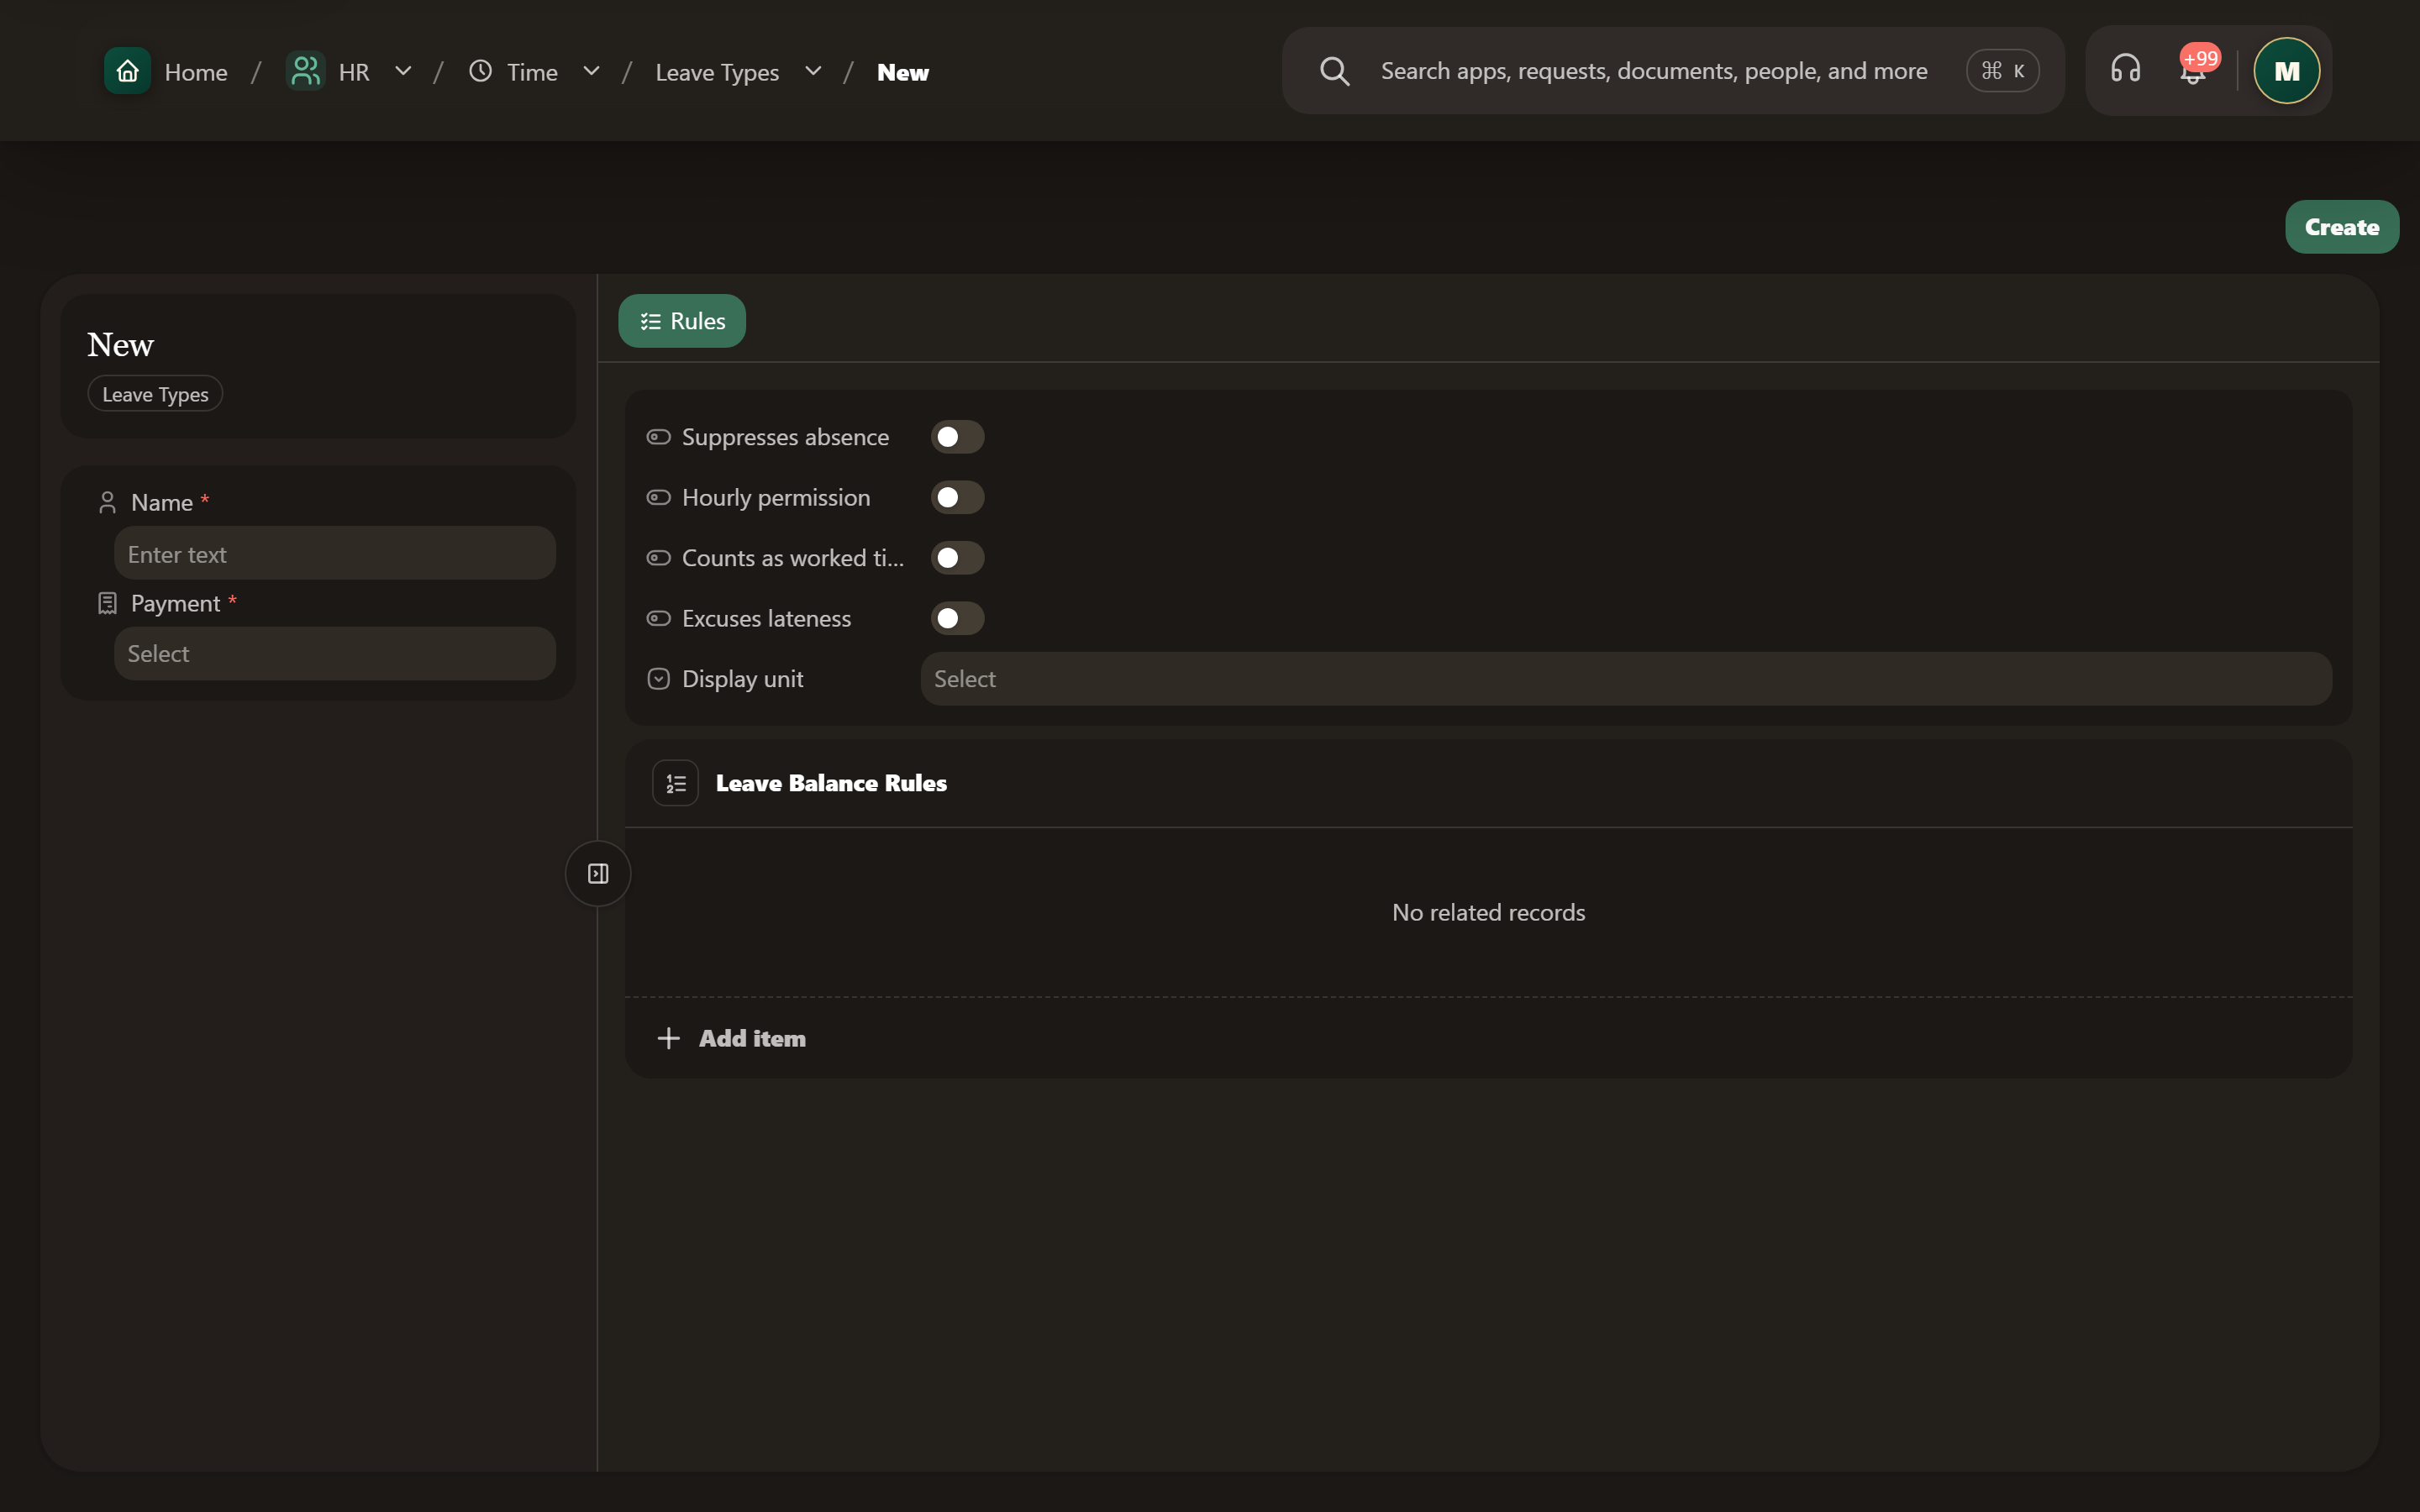
\includegraphics[width=0.95\linewidth]{figures/screens/ch03-leave-type-fields-en.png}
\caption{Leave Types: payment and rules; not saved}
\label{fig:hr-feature-leave-types-screen}
\end{figure}

\begin{table}[H]
\centering
\caption{What do you record in a leave type?}
\label{tab:hr-feature-leave-types-data}
\rcZebra
\begin{tabularx}{\linewidth}{R{3.6cm} Y}
\rcHeaderRow
\thh{Tab or field} & \thh{What do you add?}\\
Name & \req{}; for example annual paid, sick, hourly permission.\\
Payment & \req{}: Paid, Unpaid, or Partially Paid with the payment percentage.\\
Rules & Suppresses absence, hourly permission, counts as worked time, excuses lateness, display unit.\\
Leave Balance Rules & Assigned to, days or hours and their amount, frequency: weekly, monthly, yearly or once, expiry, effective date, status.\\
\end{tabularx}
\end{table}

A balance comes from a balance rule and who it is assigned to; the type alone does not give everyone a balance. A type used by leaves cannot be deleted.

\begin{figure}[H]
\centering
\begin{tikzpicture}[node distance=0.5cm,stepBox/.append style={minimum width=6.5cm,text width=6.1cm,minimum height=0.8cm}]
  \node[stepBox] (a) {Define the leave type};
  \node[stepBox,below=of a] (b) {Balance rule and who};
  \node[stepBox,below=of b] (c) {Record a dated leave};
  \draw[flowsTo] (a) -- (b);
  \draw[flowsTo] (b) -- (c);
\end{tikzpicture}
\rclegend
\caption{Steps of use; arrows do not mean automatic processing}
\label{fig:hr-feature-leave-types-flow}
\end{figure}

\subsection{Try it and check}

\begin{enumerate}
  \item Open Leave Types and search for the type before adding it.
  \item If authorized, add “Annual (paid)”, choose “Paid”, then save.
  \item In the “Rules” tab add a balance rule: assigned to, “Days”, the amount, “Yearly”, expiry, effective date, “Active”. Save.
\end{enumerate}

\textbf{Check:} reopen it and review the payment and rule. The balance appears in the member file, Attendance tab.

\begin{figure}[H]
\centering
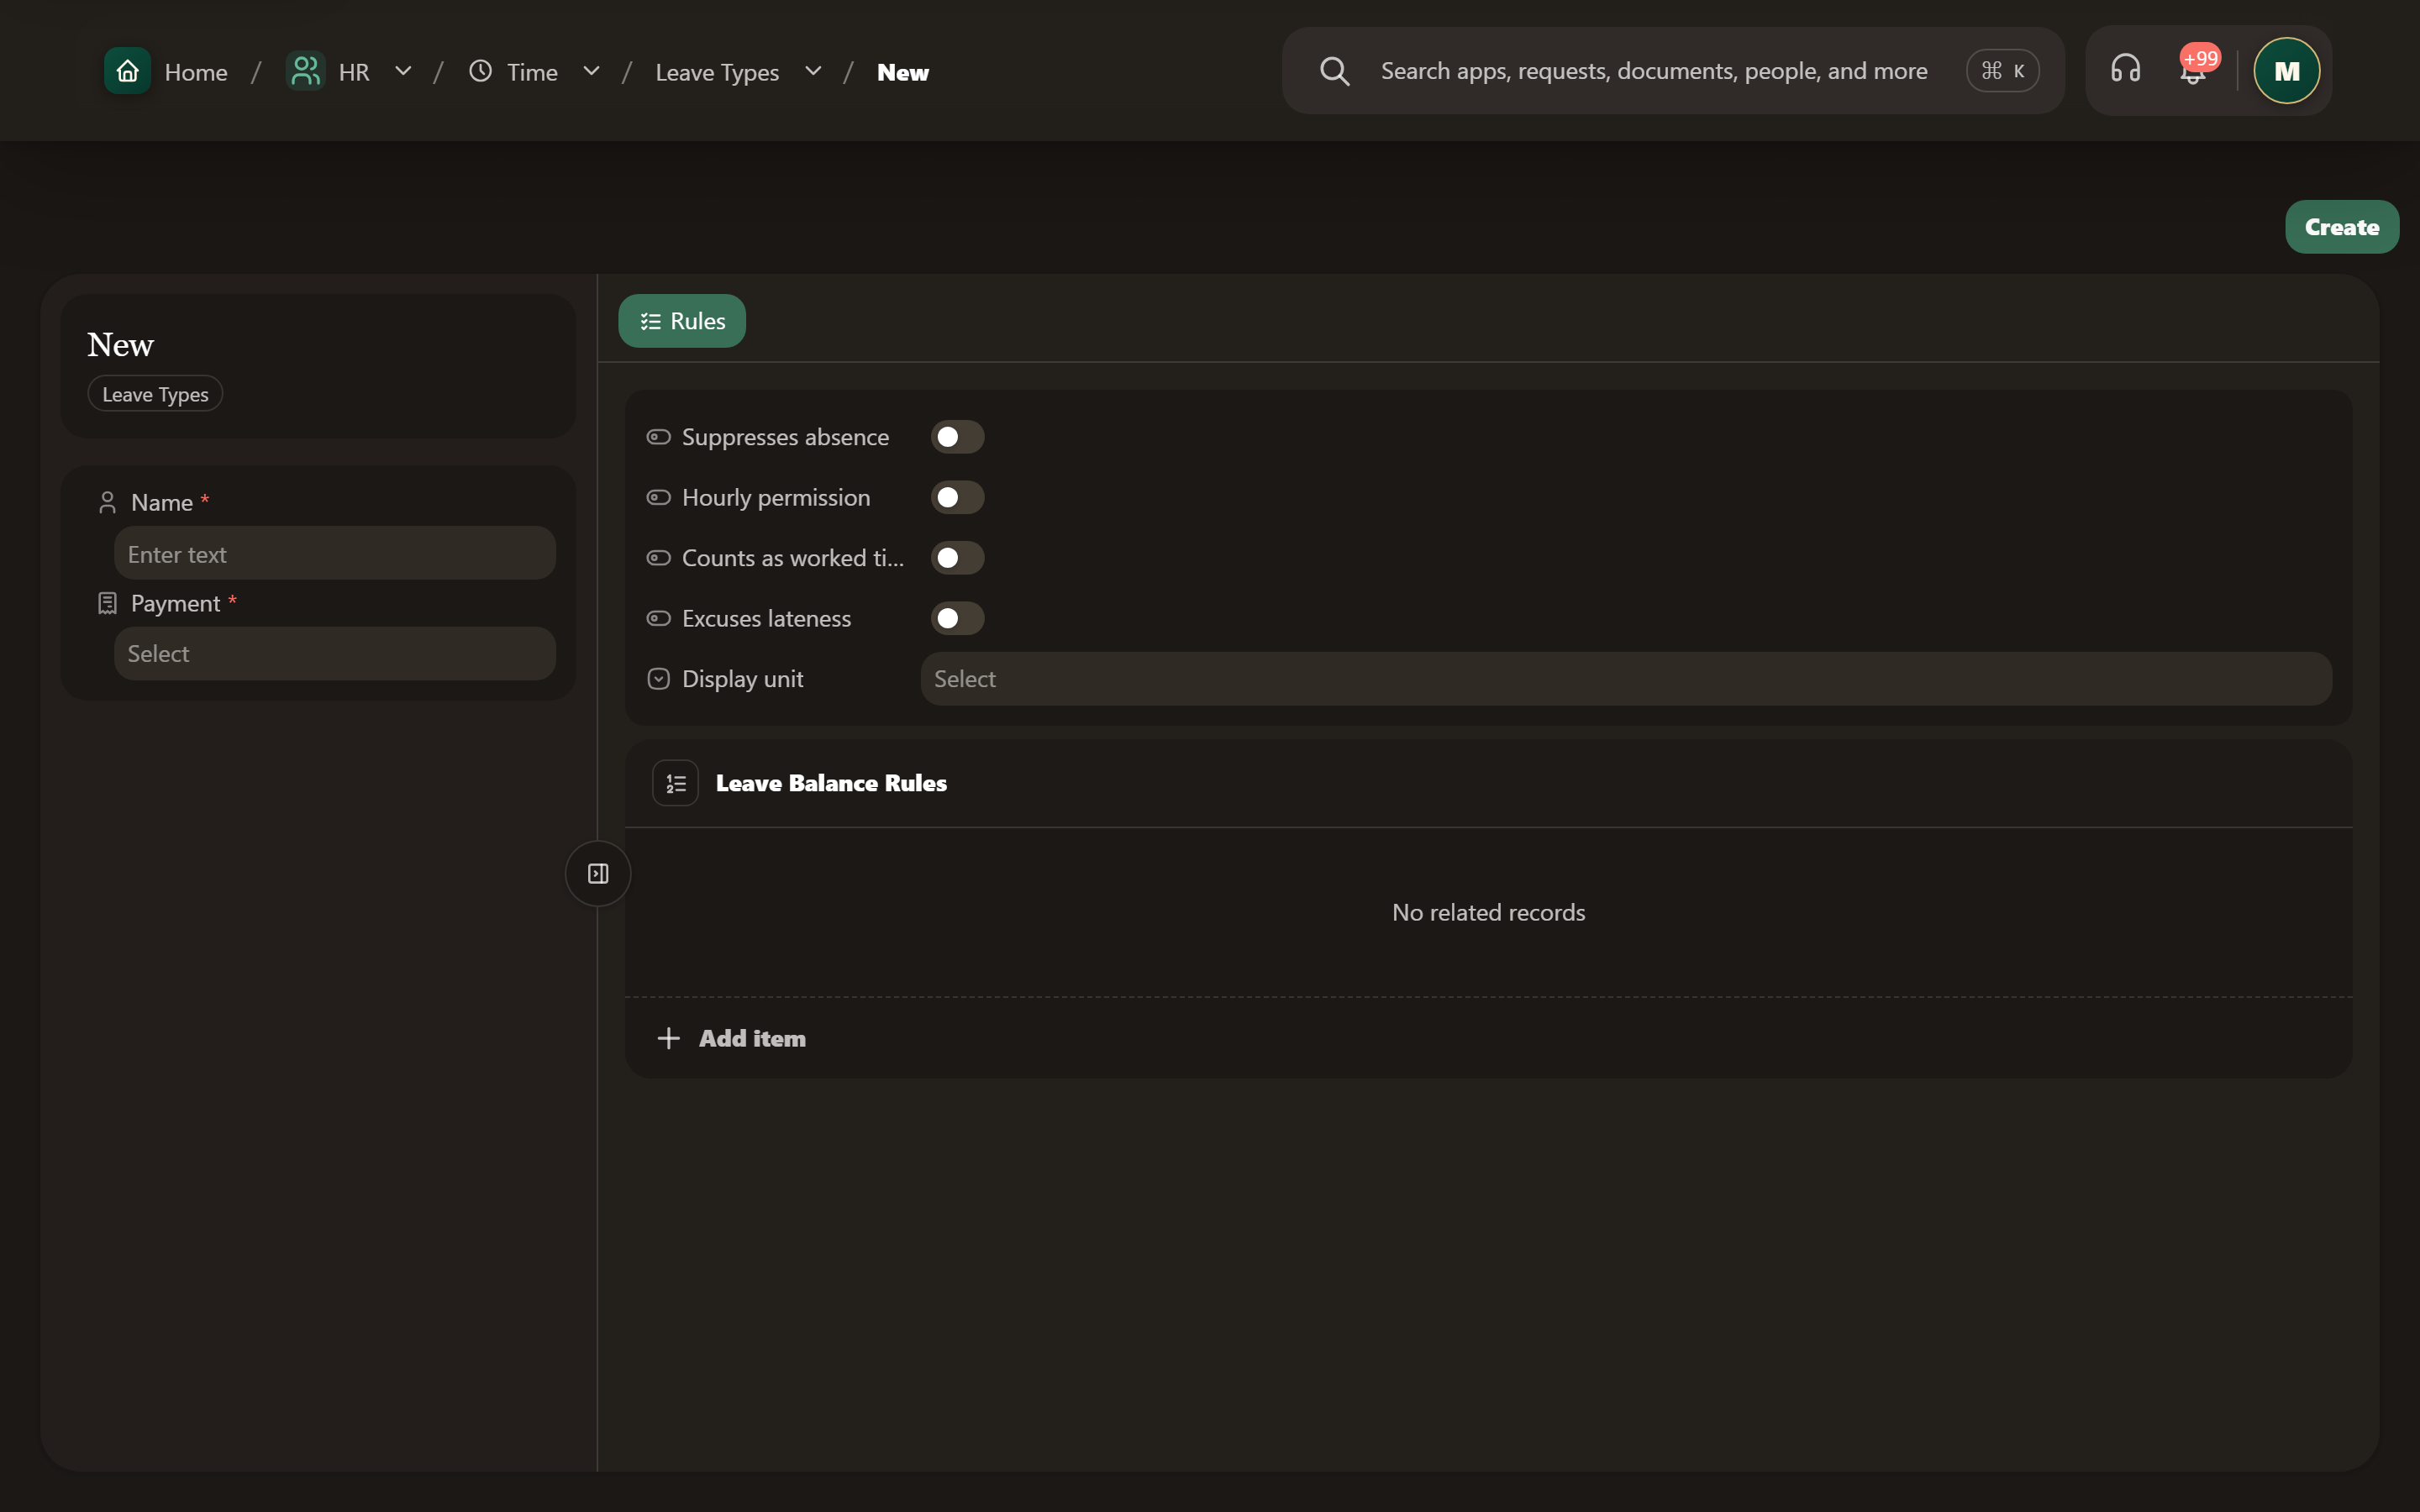
\includegraphics[width=0.95\linewidth]{figures/screens/ch03-leave-type-fields-tab1-en.png}
\caption{Rules tab in full; unsaved form}
\label{fig:hr-leave-types-fulltab1}
\end{figure}

\clearpage
\section{Leaves}
\label{sec:hr-feature-leaves}

A leave record applies a type to an employee between two dates and times, with a status: Pending, Approved or Rejected.

\textbf{When is it useful?} Record Sarah's approved absence so it shows in her attendance and pay. A holiday is shared by the team; a leave belongs to one employee. \textbf{Open:} HR / Time / Leaves.

\begin{figure}[H]
\centering
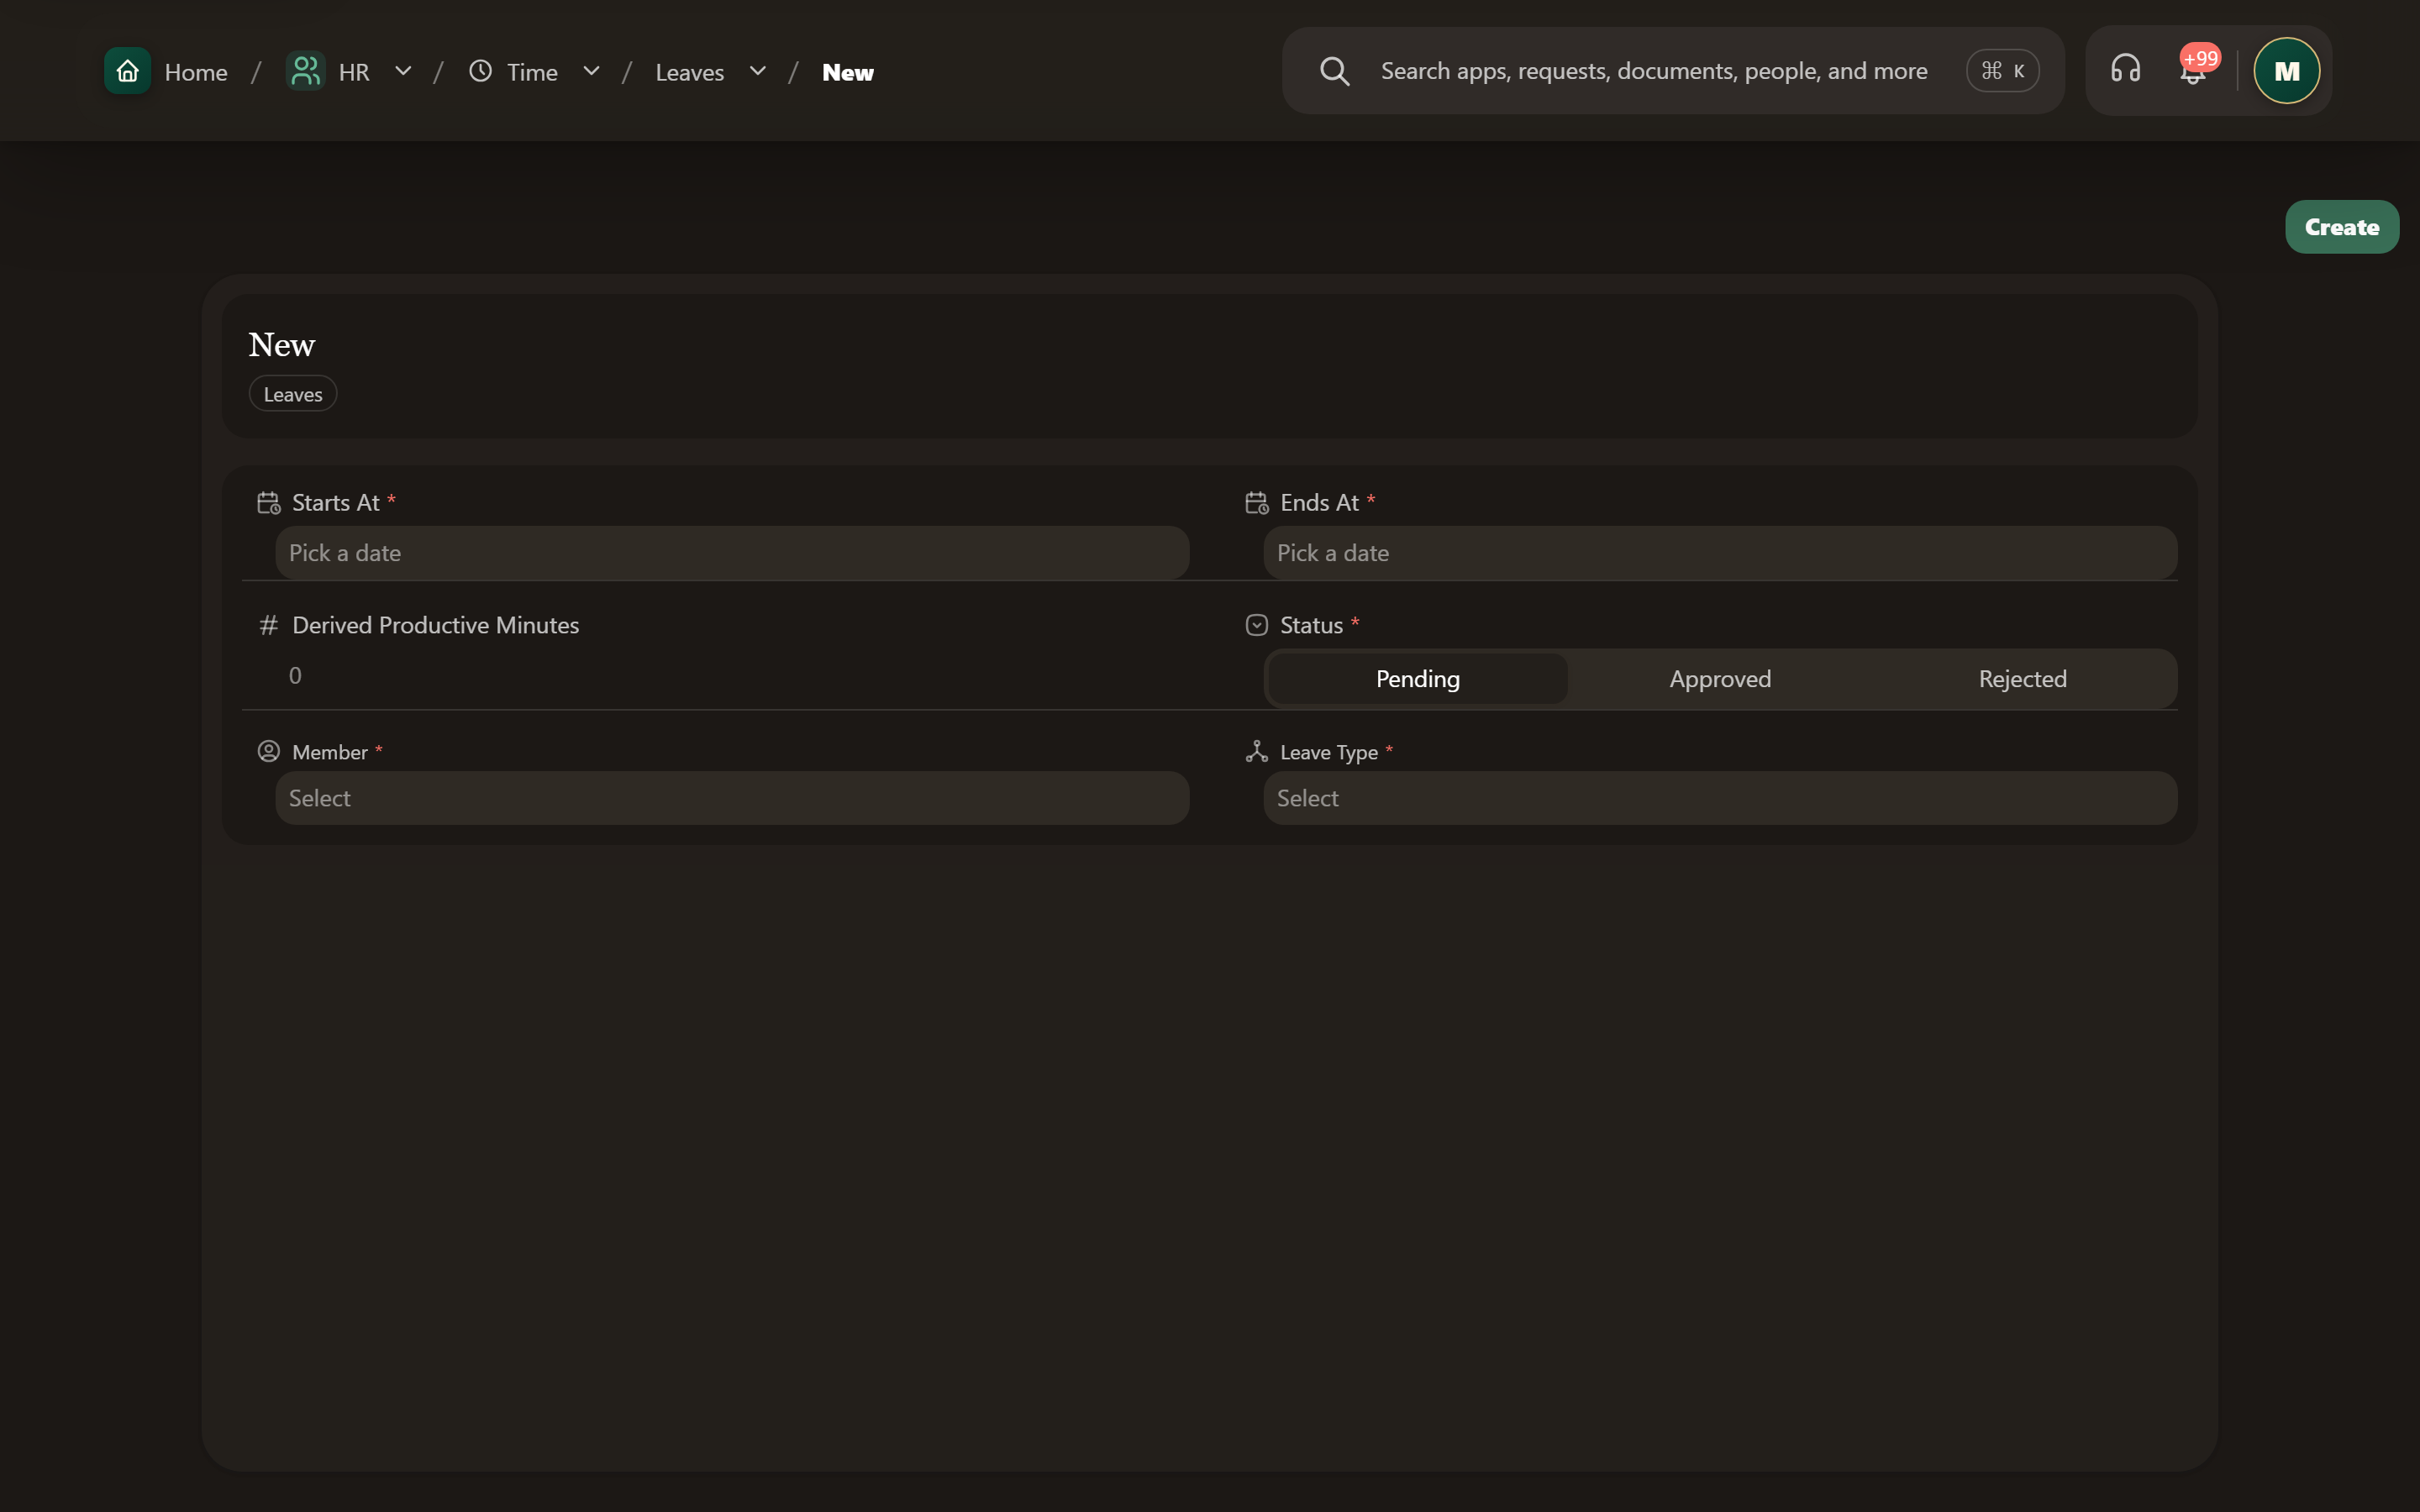
\includegraphics[width=0.95\linewidth]{figures/screens/ch03-leave-fields-en.png}
\caption{Leaves: employee, dates and status; not saved}
\label{fig:hr-feature-leaves-screen}
\end{figure}

\begin{table}[H]
\centering
\caption{What do you record in a leave?}
\label{tab:hr-feature-leaves-data}
\rcZebra
\begin{tabularx}{\linewidth}{R{3.6cm} Y}
\rcHeaderRow
\thh{Field} & \thh{What do you add?}\\
Member and Leave Type & \req{}.\\
Starts at and Ends at & \req{}: date and time.\\
Status & \req{}: Pending by default, then Approved or Rejected.\\
Derived Productive Minutes & The actual leave duration \gen{}.\\
\end{tabularx}
\end{table}

The leave also appears in the member file, Attendance tab. There is no separate approve button; the status is set on the record according to the approval.

\begin{figure}[H]
\centering
\begin{tikzpicture}[node distance=0.4cm,stepBox/.append style={minimum width=6cm,text width=5.6cm,minimum height=0.7cm}]
  \node[stepBox] (s0) {Review type and\\payment};
  \node[stepBox,below=of s0] (s1) {Obtain required\\approval};
  \node[stepBox,below=of s1] (s2) {Record employee, date\\and duration};
  \node[stepBox,below=of s2] (s3) {Save; review the day\\and pay};
  \draw[flowsTo] (s0) -- (s1);
  \draw[flowsTo] (s1) -- (s2);
  \draw[flowsTo] (s2) -- (s3);
\end{tikzpicture}
\rclegend
\caption{From leave type to reviewing the employee’s day}
\label{fig:hr-leave-flow}
\end{figure}

\subsection{Try it and check}

\begin{enumerate}
  \item Confirm the approval, dates and Sarah's balance. Open Leaves and search for an earlier record.
  \item Add: Sarah, “Annual (paid)”, the start and end times, and the status “Approved”. Save.
  \item Reopen the record and review the calculated duration, then open the day in My attendance.
\end{enumerate}

\textbf{Check:} the day shows as excused by leave. If the effect is missing, check the date, type and status; “Pending” does not excuse absence.

\clearpage
\section{Holiday Groups}
\label{sec:hr-feature-holiday-groups}

A holiday group is a shared calendar of public holidays, followed by those it is assigned to.

\textbf{When is it useful?} The team follows one holiday calendar, without recording each holiday as leave for every employee. \textbf{Open:} HR / Time / Holiday Groups.

\begin{figure}[H]
\centering
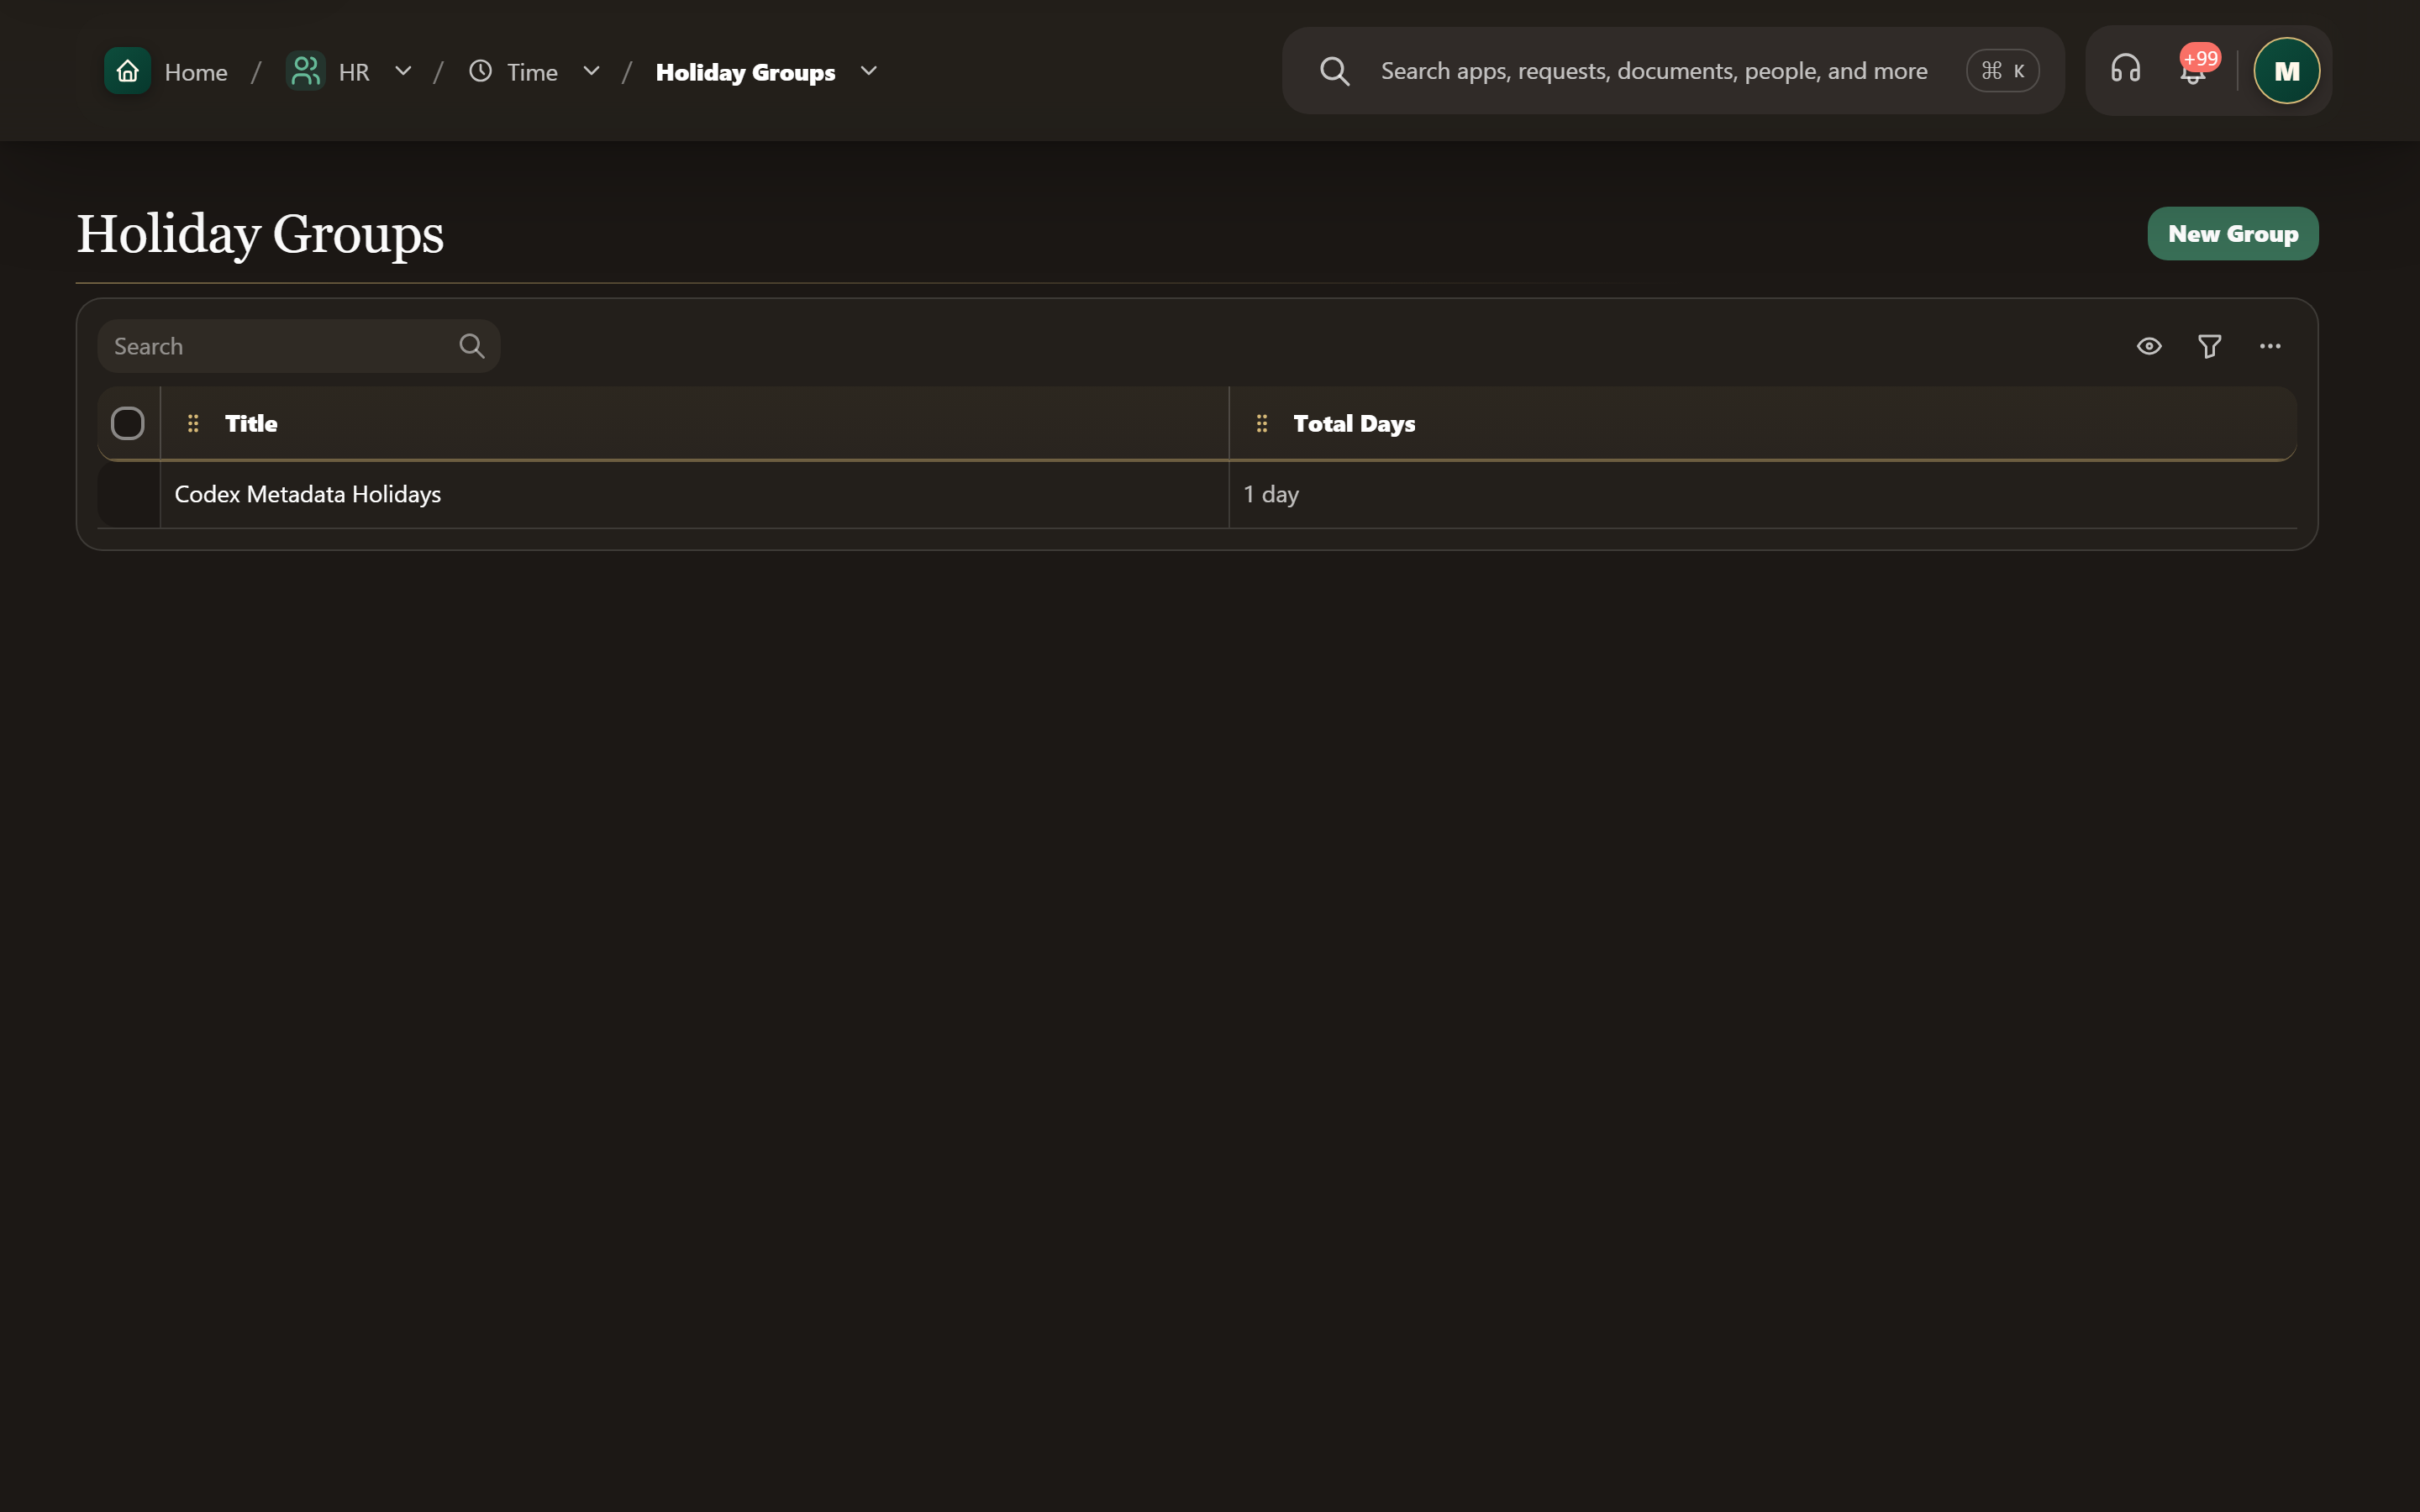
\includegraphics[width=0.95\linewidth]{figures/screens/ch03-feature-holiday-groups-en.png}
\caption{Holiday Groups: English interface in the test environment}
\label{fig:hr-feature-holiday-groups-screen}
\end{figure}

\begin{table}[H]
\centering
\caption{What do you record in a holiday group?}
\label{tab:hr-feature-holiday-groups-data}
\rcZebra
\begin{tabularx}{\linewidth}{R{3.6cm} Y}
\rcHeaderRow
\thh{Tab or field} & \thh{What do you add?}\\
Group & Group Name \req{}; holidays count and total days \gen{}.\\
Holidays & Name \req{}, then a full day with its date, a partial day with its hours, or a range from one date to another.\\
Assignee & Who follows the group: members, units or the whole organization.\\
\end{tabularx}
\end{table}

\begin{itemize}
  \item “New Group”, “Add Holiday”, and searching, editing or deleting holidays.
  \item Two holidays cannot share a date. An assignment can override its holiday groups.
\end{itemize}

\begin{figure}[H]
\centering
\begin{tikzpicture}[node distance=0.5cm,stepBox/.append style={minimum width=6.5cm,text width=6.1cm,minimum height=0.8cm}]
  \node[stepBox] (a) {Prepare the shared calendar};
  \node[stepBox,below=of a] (b) {Add holiday dates};
  \node[stepBox,below=of b] (c) {Review assignees};
  \draw[flowsTo] (a) -- (b);
  \draw[flowsTo] (b) -- (c);
\end{tikzpicture}
\rclegend
\caption{Steps of use; arrows do not mean automatic processing}
\label{fig:hr-feature-holiday-groups-flow}
\end{figure}

\subsection{Try it and check}

\begin{enumerate}
  \item Open Holiday Groups, then the right group or “New Group”.
  \item “Add Holiday”: name and date, choose full day, partial day or range, then save.
  \item In “Assignee” choose the HR unit or the whole organization, and save.
\end{enumerate}

\textbf{Check:} the holiday shows as “Holiday” in My attendance for an employee it covers.

\clearpage
\section{Attendance Corrections}
\label{sec:hr-feature-attendance-corrections}

This page gathers days that need fixing, such as a missing punch, so you can correct their punches and approve or reject the decision.

\textbf{When is it useful?} To handle the team's wrong days before payroll, instead of hunting for them day by day. \textbf{Open:} HR / Time / Attendance Corrections.

\begin{figure}[H]
\centering
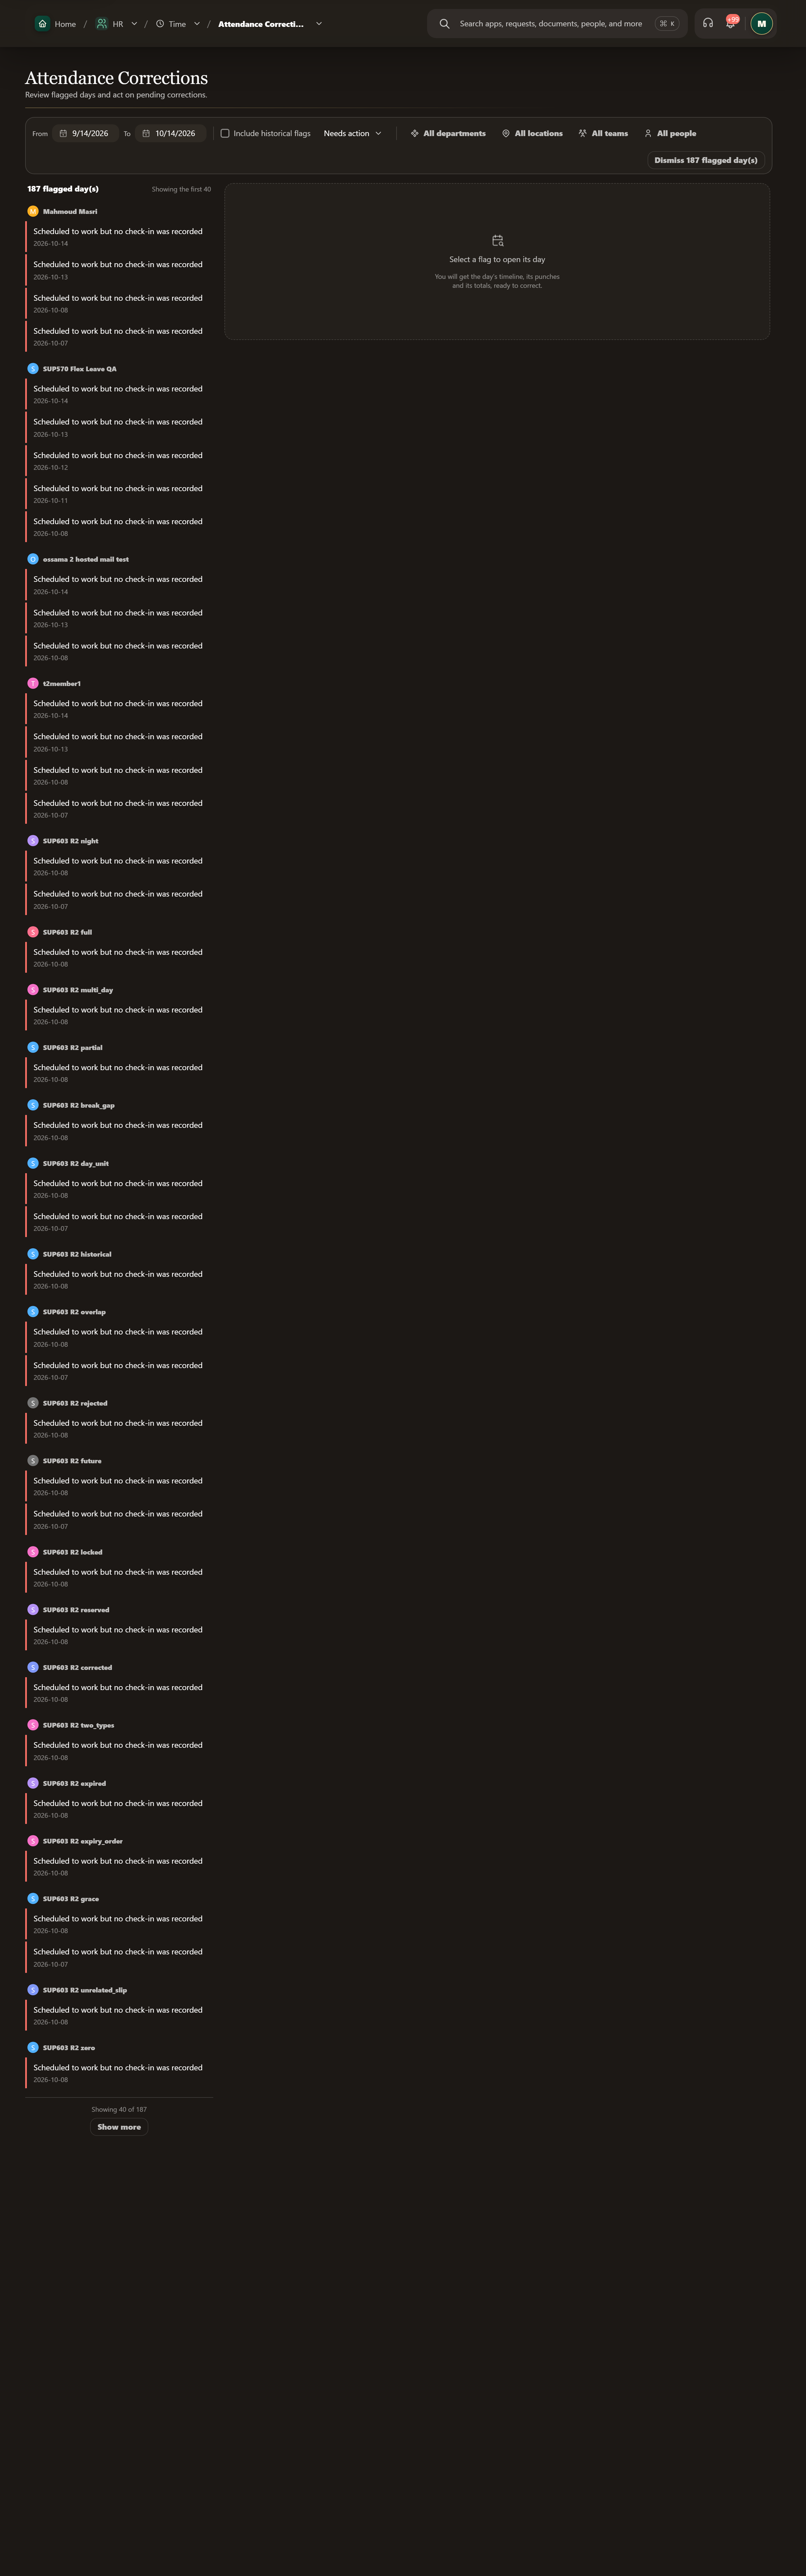
\includegraphics[width=0.95\linewidth]{figures/screens/ch03-feature-attendance-corrections-en.png}
\caption{Attendance Corrections: English interface in the test environment}
\label{fig:hr-feature-attendance-corrections-screen}
\end{figure}

\begin{table}[H]
\centering
\caption{What do you see in Attendance Corrections?}
\label{tab:hr-feature-attendance-corrections-data}
\rcZebra
\begin{tabularx}{\linewidth}{R{3.6cm} Y}
\rcHeaderRow
\thh{Part} & \thh{What does it show?}\\
Filters & From and To; Needs action, Awaiting approval, Resolved, All; departments, locations, teams and people.\\
Flag reason & No check-out, no check-in, duplicate check-in, implausible duration, punch outside the shift window, absent though scheduled.\\
Day panel & Punches and their source: device or manual; the timeline; work and breaks against the shift.\\
Request & Reason and justification, who requested it, the changes, and the approval deadline.\\
\end{tabularx}
\end{table}

\subsection{What can you do?}

\begin{itemize}
  \item Add a punch, change its time or direction, or remove it. For a day with no punches: “Register leave”.
  \item “Save correction”, “Send for approval”, “Approve”, “Reject”; depending on your role.
  \item Dismiss a flag: “Confirm absence” or “Not an issue”. For bulk dismiss, type the number to confirm.
  \item The correction deadline is set at the bottom of the Attendance policy page.
\end{itemize}

\begin{figure}[H]
\centering
\begin{tikzpicture}[node distance=0.5cm,stepBox/.append style={minimum width=6.5cm,text width=6.1cm,minimum height=0.8cm}]
  \node[stepBox] (a) {Review the day};
  \node[stepBox,below=of a] (b) {Send the correction};
  \node[stepBox,below=of b] (c) {Review decision and day};
  \draw[flowsTo] (a) -- (b);
  \draw[flowsTo] (b) -- (c);
\end{tikzpicture}
\rclegend
\caption{Steps of use; arrows do not mean automatic processing}
\label{fig:hr-feature-attendance-corrections-flow}
\end{figure}

\subsection{Try it and check}

\begin{enumerate}
  \item Open Attendance Corrections, choose “Needs action” and the HR unit.
  \item Open the day, add the missing punch, choose the reason, then “Send for approval”.
\end{enumerate}

\textbf{Check:} the day moves to “Awaiting approval”, then “Resolved” after the decision. If the action is unavailable, check the deadline and permissions.

\clearpage
\section{Attendance policy}
\label{sec:hr-feature-attendance-policy}

An attendance policy is a set of rules that evaluates recorded time: when lateness is forgiven, when time counts as overtime, and who it applies to.

\textbf{When is it useful?} Consistent attendance review. The shift sets expected time; the policy evaluates the difference. \textbf{Open:} HR / Time / Attendance policy.

\begin{figure}[H]
\centering
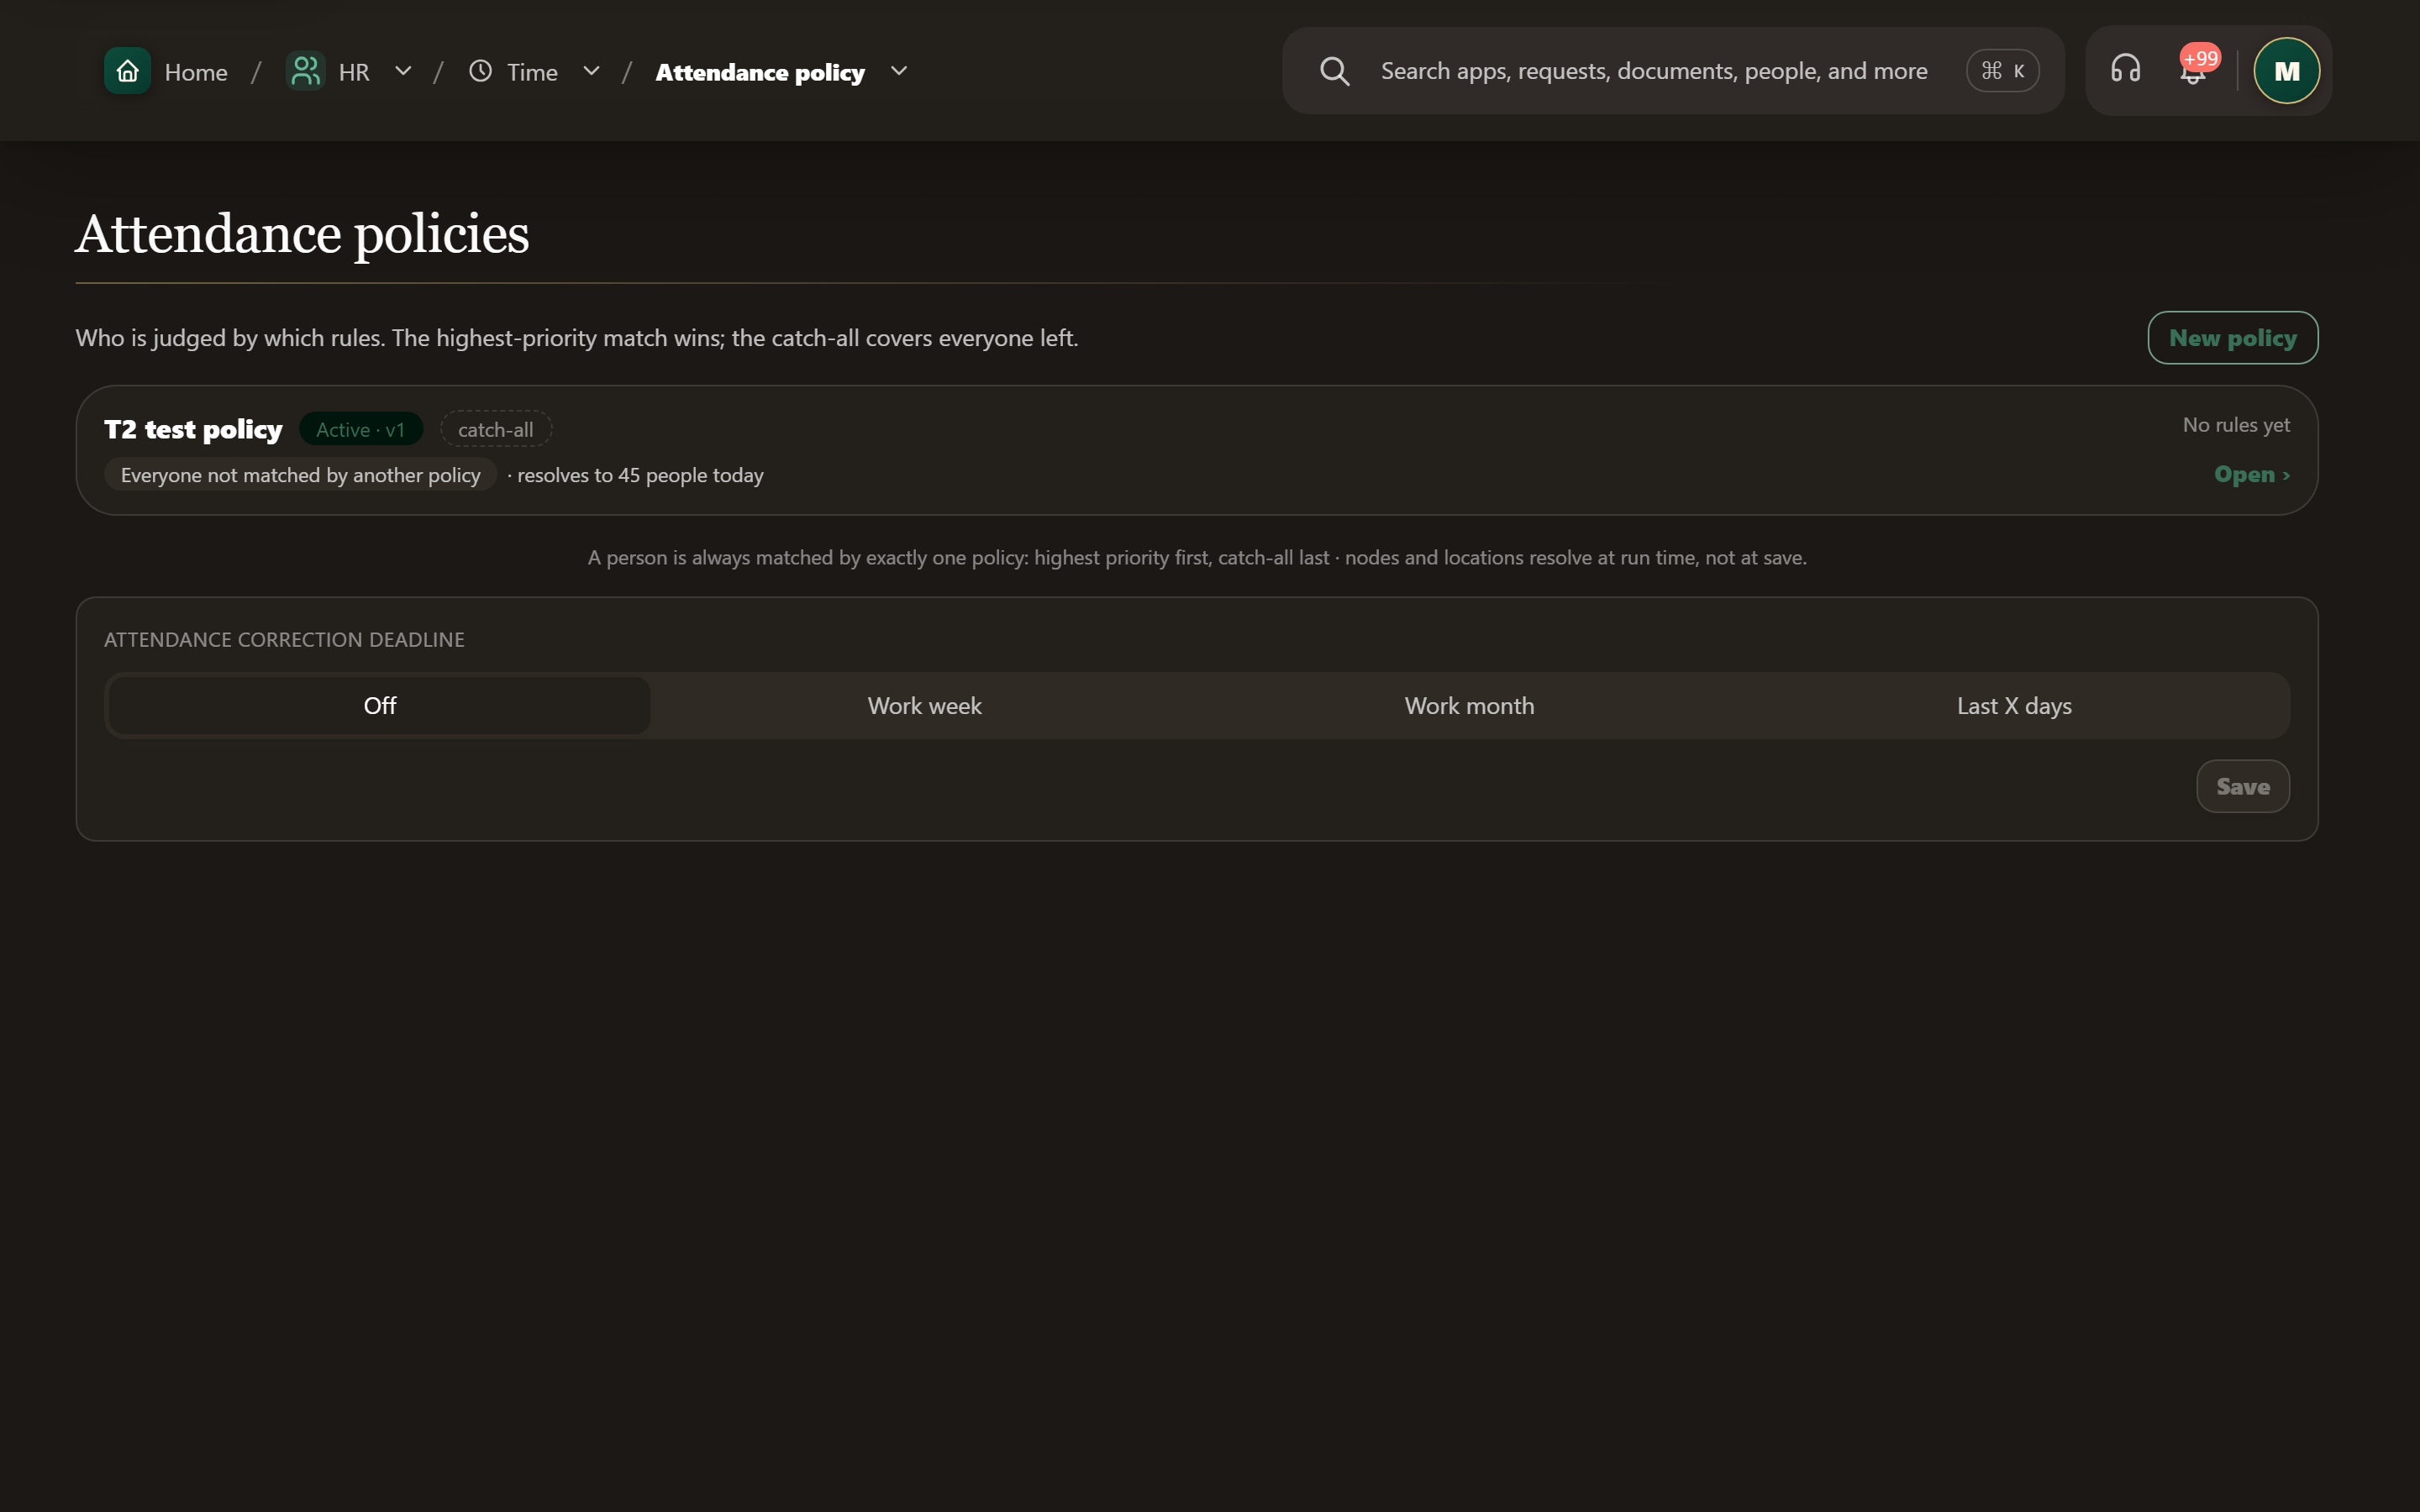
\includegraphics[width=0.95\linewidth]{figures/screens/ch03-feature-attendance-policy-en.png}
\caption{Attendance policy: English interface in the test environment}
\label{fig:hr-feature-attendance-policy-screen}
\end{figure}

\begin{table}[H]
\centering
\caption{What do you set in a policy?}
\label{tab:hr-feature-attendance-policy-data}
\rcZebra
\begin{tabularx}{\linewidth}{R{3.6cm} Y}
\rcHeaderRow
\thh{Tab or part} & \thh{What do you set?}\\
Assigned to & People, units, locations, positions or groups. The catch-all policy covers everyone no other policy matches.\\
Minute rules & Late arrival, early leave, break overrun, shortfall, overtime.\\
Whole-day rules & Absence, rest-day work, holiday work.\\
Bands & From X to Y minutes: forgive or count with a multiplier, and record as a category such as “Late — forgiven”.\\
Status & Draft, Active with a version, Disabled; and priority: the highest match wins.\\
\end{tabularx}
\end{table}

\subsection{What can you do?}

\begin{itemize}
  \item “Create a policy”, which starts as a draft, then “Edit rules”, “Save draft” and “Activate”.
  \item “Try a time” for late arrival: pick a shift and an arrival time and see the result.
  \item “Simulate”: “Replay last month” with the draft before activating it.
  \item “Disable policy”, and “Delete policy” if it was never enabled.
\end{itemize}

\begin{figure}[H]
\centering
\begin{tikzpicture}[node distance=0.5cm,stepBox/.append style={minimum width=6.5cm,text width=6.1cm,minimum height=0.8cm}]
  \node[stepBox] (a) {Choose the policy scope};
  \node[stepBox,below=of a] (b) {Review attendance rules};
  \node[stepBox,below=of b] (c) {Check a trial result};
  \draw[flowsTo] (a) -- (b);
  \draw[flowsTo] (b) -- (c);
\end{tikzpicture}
\rclegend
\caption{Steps of use; arrows do not mean automatic processing}
\label{fig:hr-feature-attendance-policy-flow}
\end{figure}

\subsection{Try it and check}

\begin{enumerate}
  \item The authorized administrator opens Attendance policy, chooses the policy, then “Edit rules”.
  \item In late arrival add a band: from 0 to 10 minutes is forgiven. Save the draft.
  \item Use “Try a time” and “Simulate”, then “Activate” when the result is right.
\end{enumerate}

\textbf{Check:} review a real day in My attendance after activation. A warning flag alone does not mean a pay deduction.

\clearpage
\section{Attendance terminals}
\label{sec:hr-feature-attendance-terminals}

This page connects fingerprint devices to the system. Each site has a network, and an attendance agent on that network sends punches automatically; they are then matched to employees.

\textbf{When is it useful?} When attendance comes from a physical device. A device in the list does not prove its punches arrive. \textbf{Open:} HR / Time / Attendance terminals.

\begin{figure}[H]
\centering
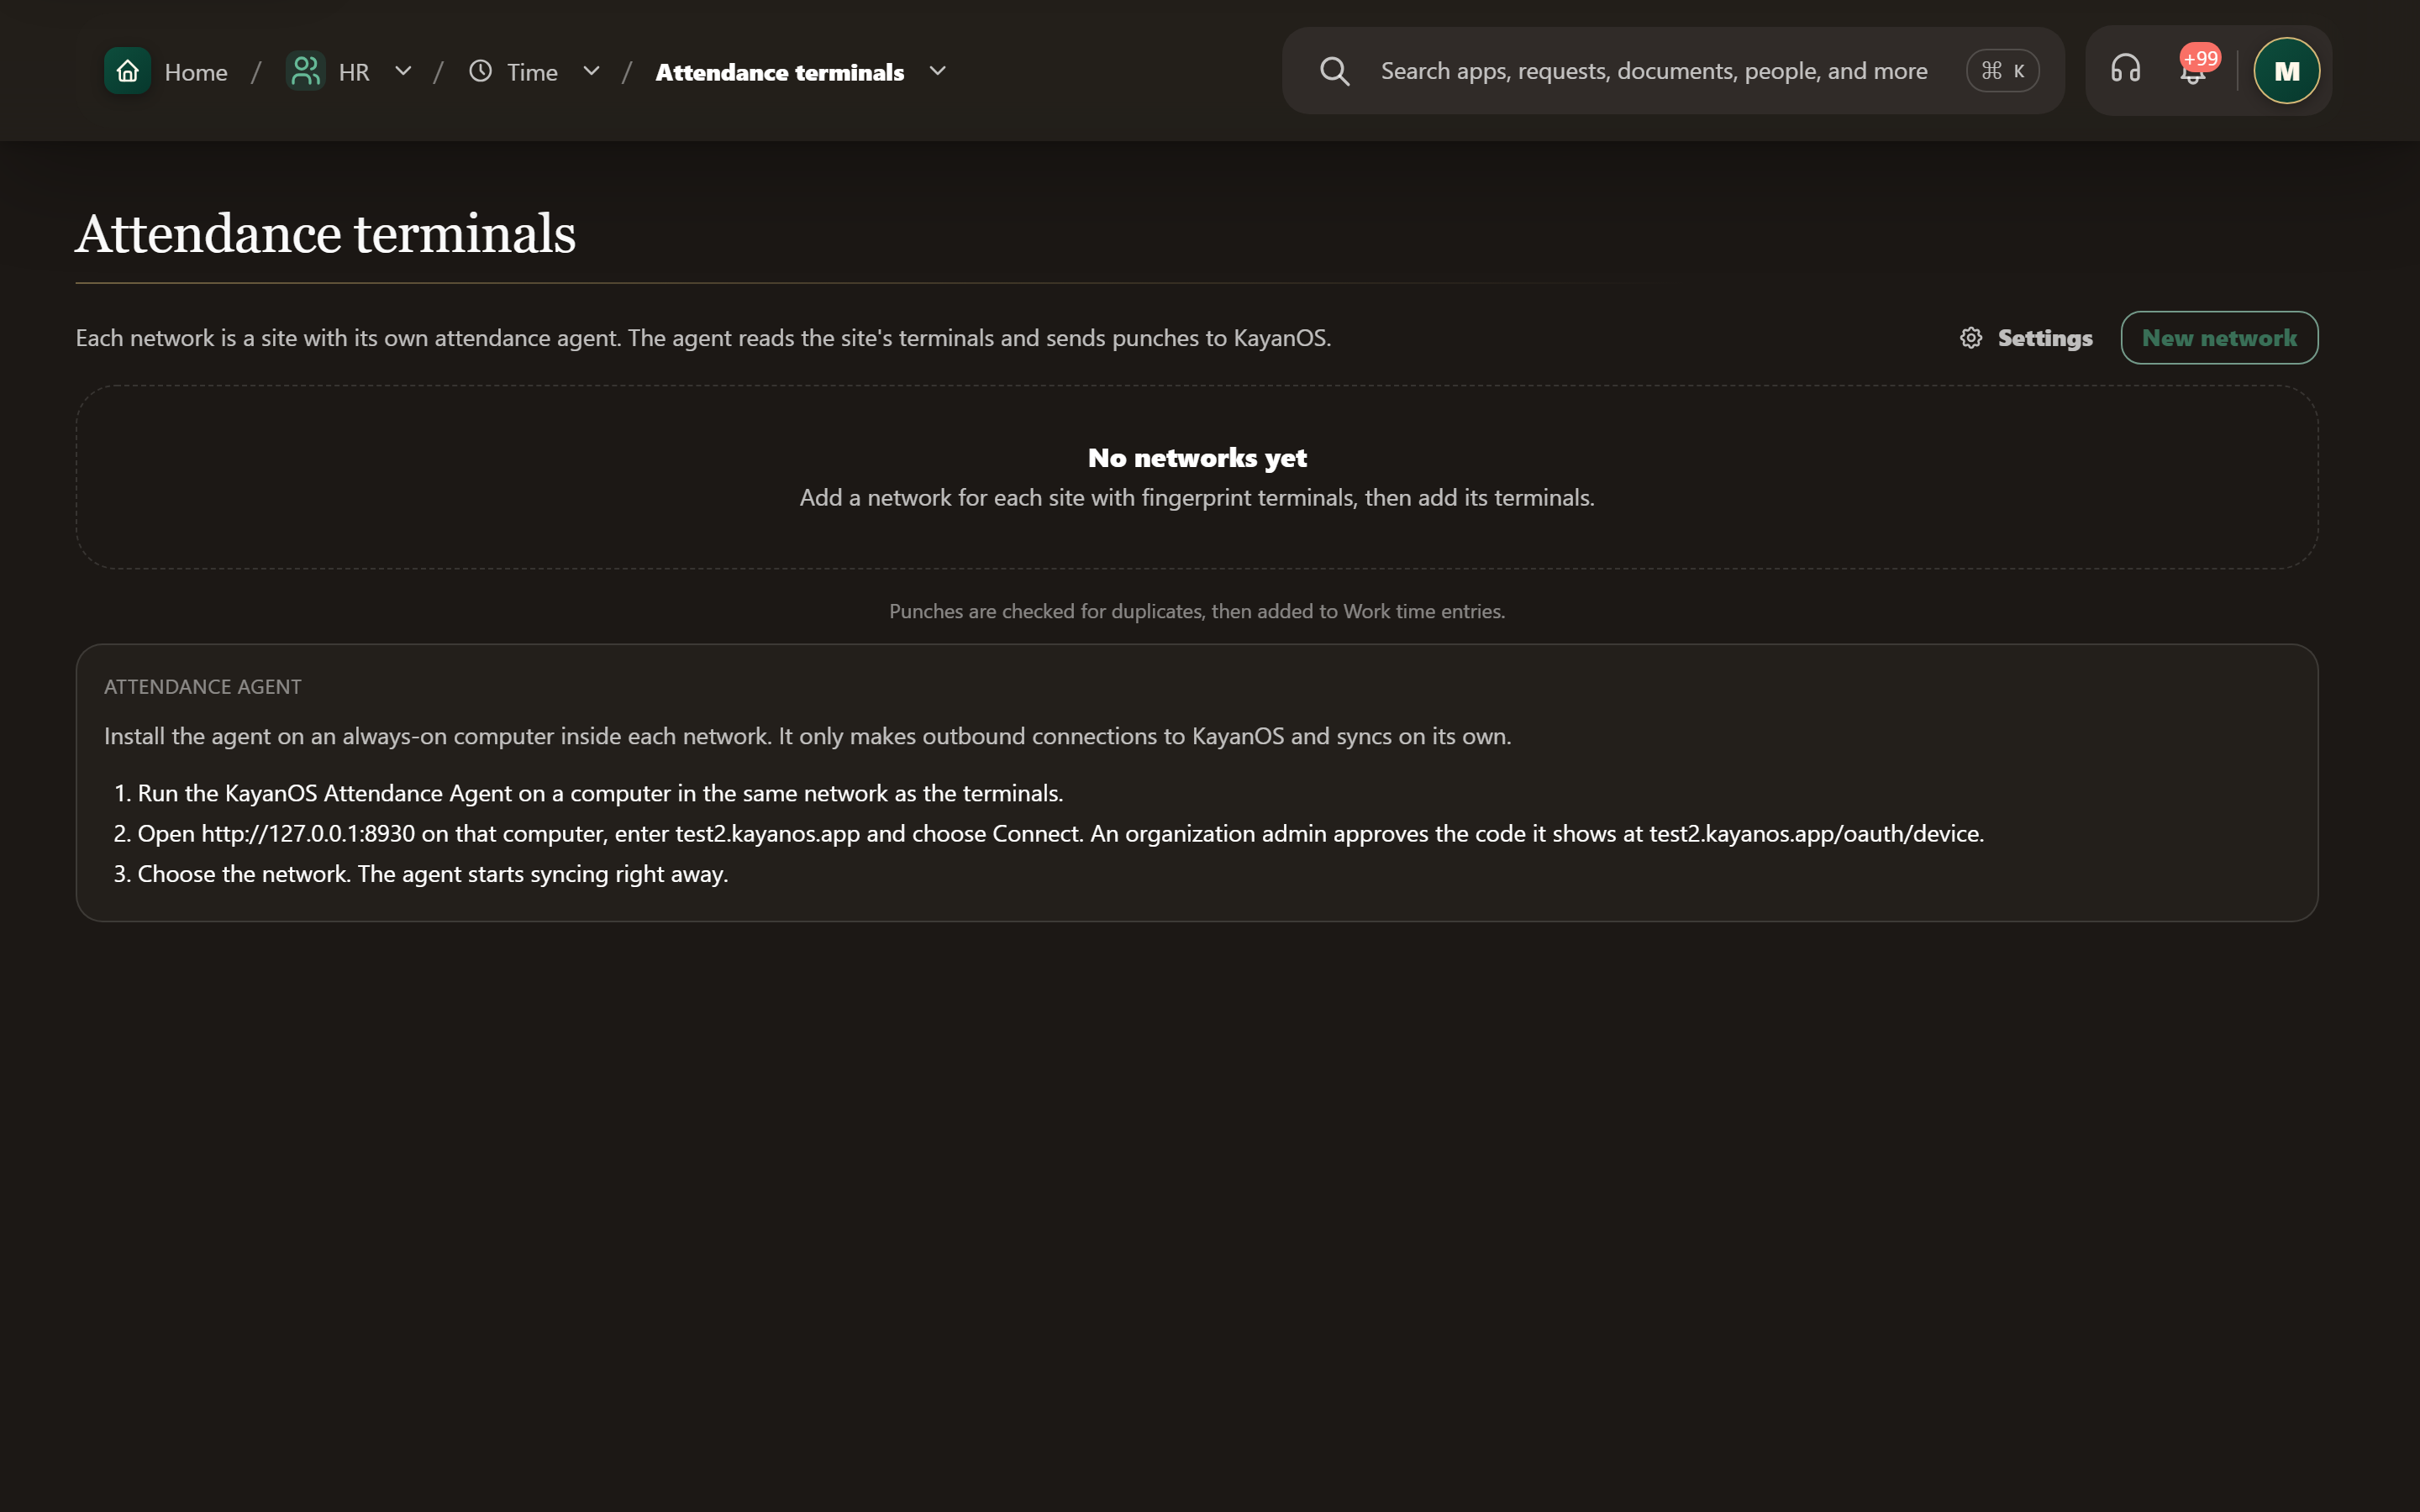
\includegraphics[width=0.95\linewidth]{figures/screens/ch03-feature-attendance-terminals-en.png}
\caption{Attendance terminals: English interface in the test environment}
\label{fig:hr-feature-attendance-terminals-screen}
\end{figure}

\begin{table}[H]
\centering
\caption{What do you record in Attendance terminals?}
\label{tab:hr-feature-attendance-terminals-data}
\rcZebra
\begin{tabularx}{\linewidth}{R{3.6cm} Y}
\rcHeaderRow
\thh{Part} & \thh{What do you add or see?}\\
Network & Name \req{}, location, timezone, sync every 5–60 minutes.\\
Terminal & Name, IP address and port \req{} (4370 by default), communication key, punch direction.\\
Device details & Model, enrolled users, capacity, terminal clock and drift, last punch \gen{}.\\
Settings & Import punches from a date, and automatic matching by member code or manual matching.\\
\end{tabularx}
\end{table}

\subsection{What can you do?}

\begin{itemize}
  \item “New network”, then “Add terminal”.
  \item Network tabs: Terminals, Sync runs, Unmatched punches with “Assign to member”, Agent with “Disconnect agent”.
  \item The agent runs the sync; there is no manual sync button.
\end{itemize}

\begin{figure}[H]
\centering
\begin{tikzpicture}[node distance=0.5cm,stepBox/.append style={minimum width=6.5cm,text width=6.1cm,minimum height=0.8cm}]
  \node[stepBox] (a) {Check the device};
  \node[stepBox,below=of a] (b) {Match users\\to members};
  \node[stepBox,below=of b] (c) {Review a punch};
  \draw[flowsTo] (a) -- (b);
  \draw[flowsTo] (b) -- (c);
\end{tikzpicture}
\rclegend
\caption{Steps of use; arrows do not mean automatic processing}
\label{fig:hr-feature-attendance-terminals-flow}
\end{figure}

\subsection{Try it and check}

\begin{enumerate}
  \item The organization administrator opens Attendance terminals, then the site's network. For a new site: “New network”, then “Add terminal”.
  \item Review the agent status and last sync. In “Unmatched punches”, link each device user to their member.
\end{enumerate}

\textbf{Check:} compare a known punch with the employee's day in My attendance. If missing, check the agent, matching and timezone.

\clearpage
\section{Seniority Levels}
\label{sec:hr-feature-seniority-levels}

A seniority level is a grade in the salary scale, with a rank, two salary limits and an experience group.

\textbf{When is it useful?} A consistent pay reference: each position has a grade. A grade is not a person or a slip. \textbf{Open:} HR / Salary Scale / Seniority Levels.

\begin{figure}[H]
\centering
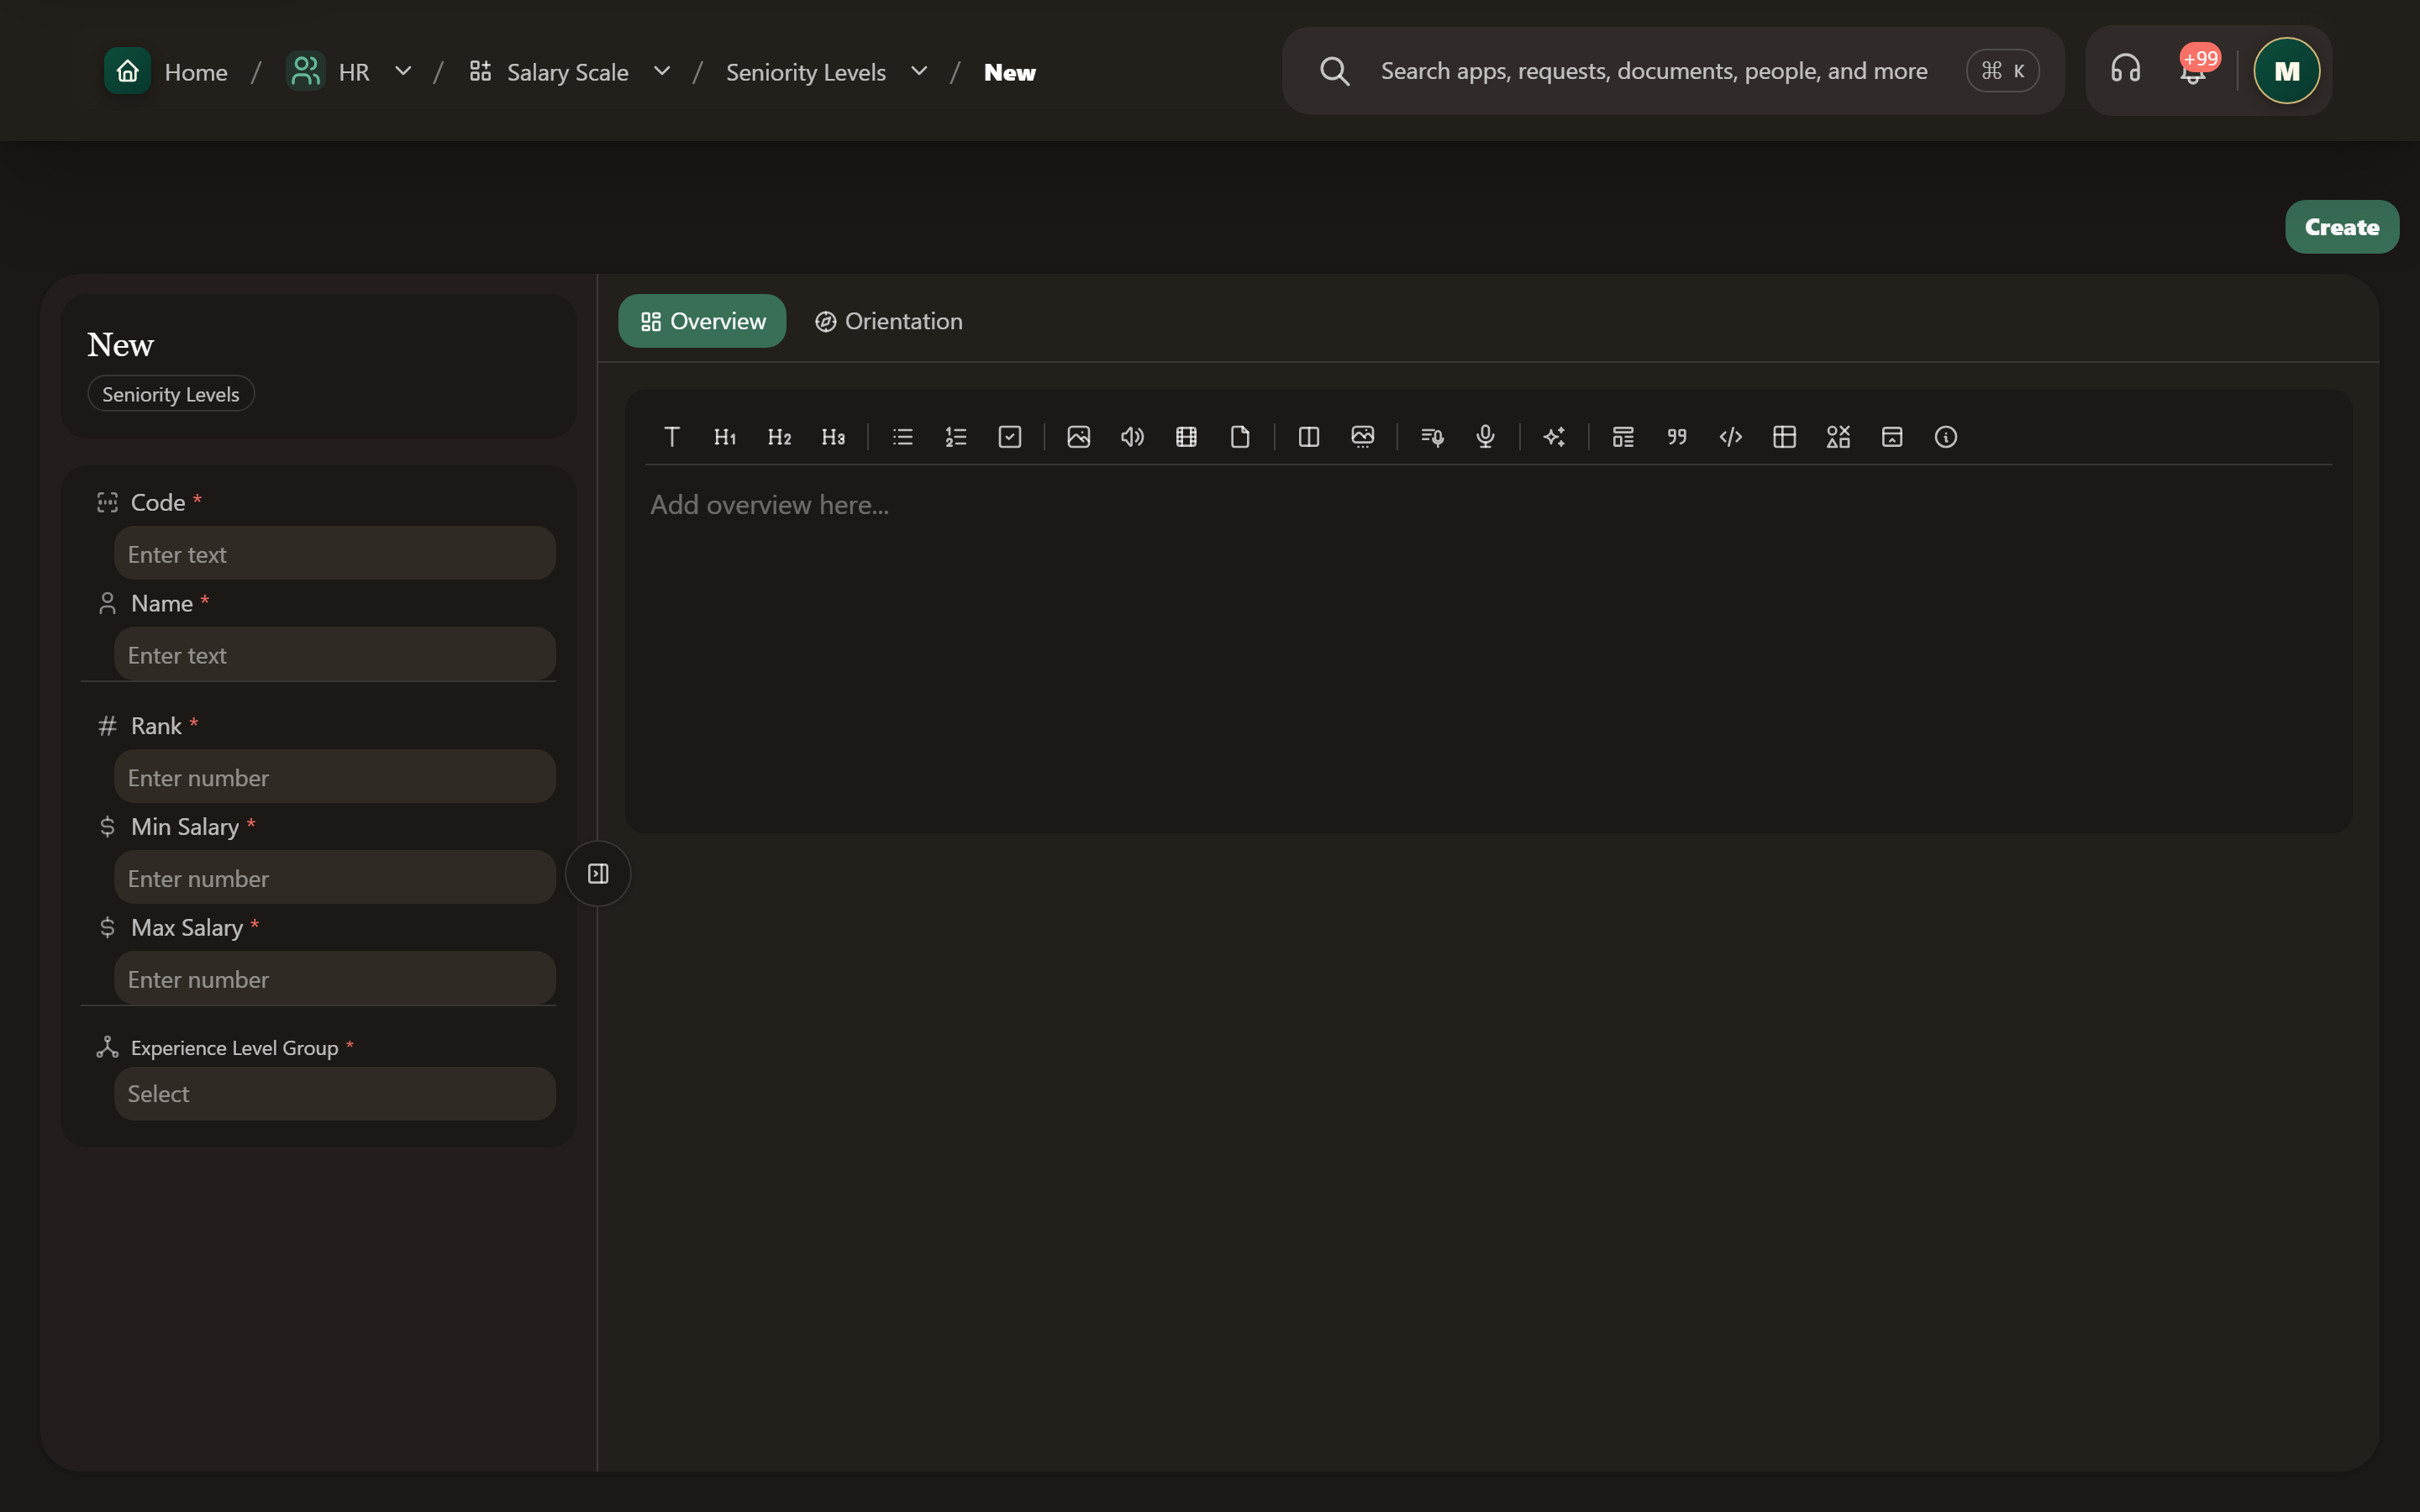
\includegraphics[width=0.95\linewidth]{figures/screens/ch03-feature-seniority-levels-en.png}
\caption{Seniority Levels: Unsaved form in the test environment}
\label{fig:hr-feature-seniority-levels-screen}
\end{figure}

\begin{table}[H]
\centering
\caption{What do you record in a seniority level?}
\label{tab:hr-feature-seniority-levels-data}
\rcZebra
\begin{tabularx}{\linewidth}{R{3.6cm} Y}
\rcHeaderRow
\thh{Field} & \thh{What do you add?}\\
Name and Code & \req{}; the code must be unique.\\
Rank & \req{}: a unique number that orders the grades.\\
Starting Salary and Max Salary & \req{}: the grade's first and highest salary.\\
Experience Level Group & \req{}: the raises added to the starting salary.\\
\end{tabularx}
\end{table}

A position links to a seniority level. The system suggests the assignment salary from the starting salary and experience steps \gen{}.

\begin{figure}[H]
\centering
\begin{tikzpicture}[node distance=0.5cm,stepBox/.append style={minimum width=6.5cm,text width=6.1cm,minimum height=0.8cm}]
  \node[stepBox] (a) {Define the job grade};
  \node[stepBox,below=of a] (b) {Review the pay reference};
  \node[stepBox,below=of b] (c) {Check assignment pay};
  \draw[flowsTo] (a) -- (b);
  \draw[flowsTo] (b) -- (c);
\end{tikzpicture}
\rclegend
\caption{Steps of use; arrows do not mean automatic processing}
\label{fig:hr-feature-seniority-levels-flow}
\end{figure}

\subsection{Try it and check}

\begin{enumerate}
  \item Prepare the experience group first. Open Seniority Levels and add the grade.
  \item Complete name, code, rank, starting and max salary and the experience group with approved values, then save.
\end{enumerate}

\textbf{Check:} open the Salary Scale and review the grade's row. Link the grade to the position, then review the assignment pay.

\clearpage
\section{Experience Levels}
\label{sec:hr-feature-experience-levels}

Here you manage experience groups: each group has ordered levels and a rule that raises the salary from one level to the next.

\textbf{When is it useful?} Consistent experience steps for the salary scale. Order matters; renaming a level does not move it. \textbf{Open:} HR / Salary Scale / Experience Levels.

\begin{figure}[H]
\centering
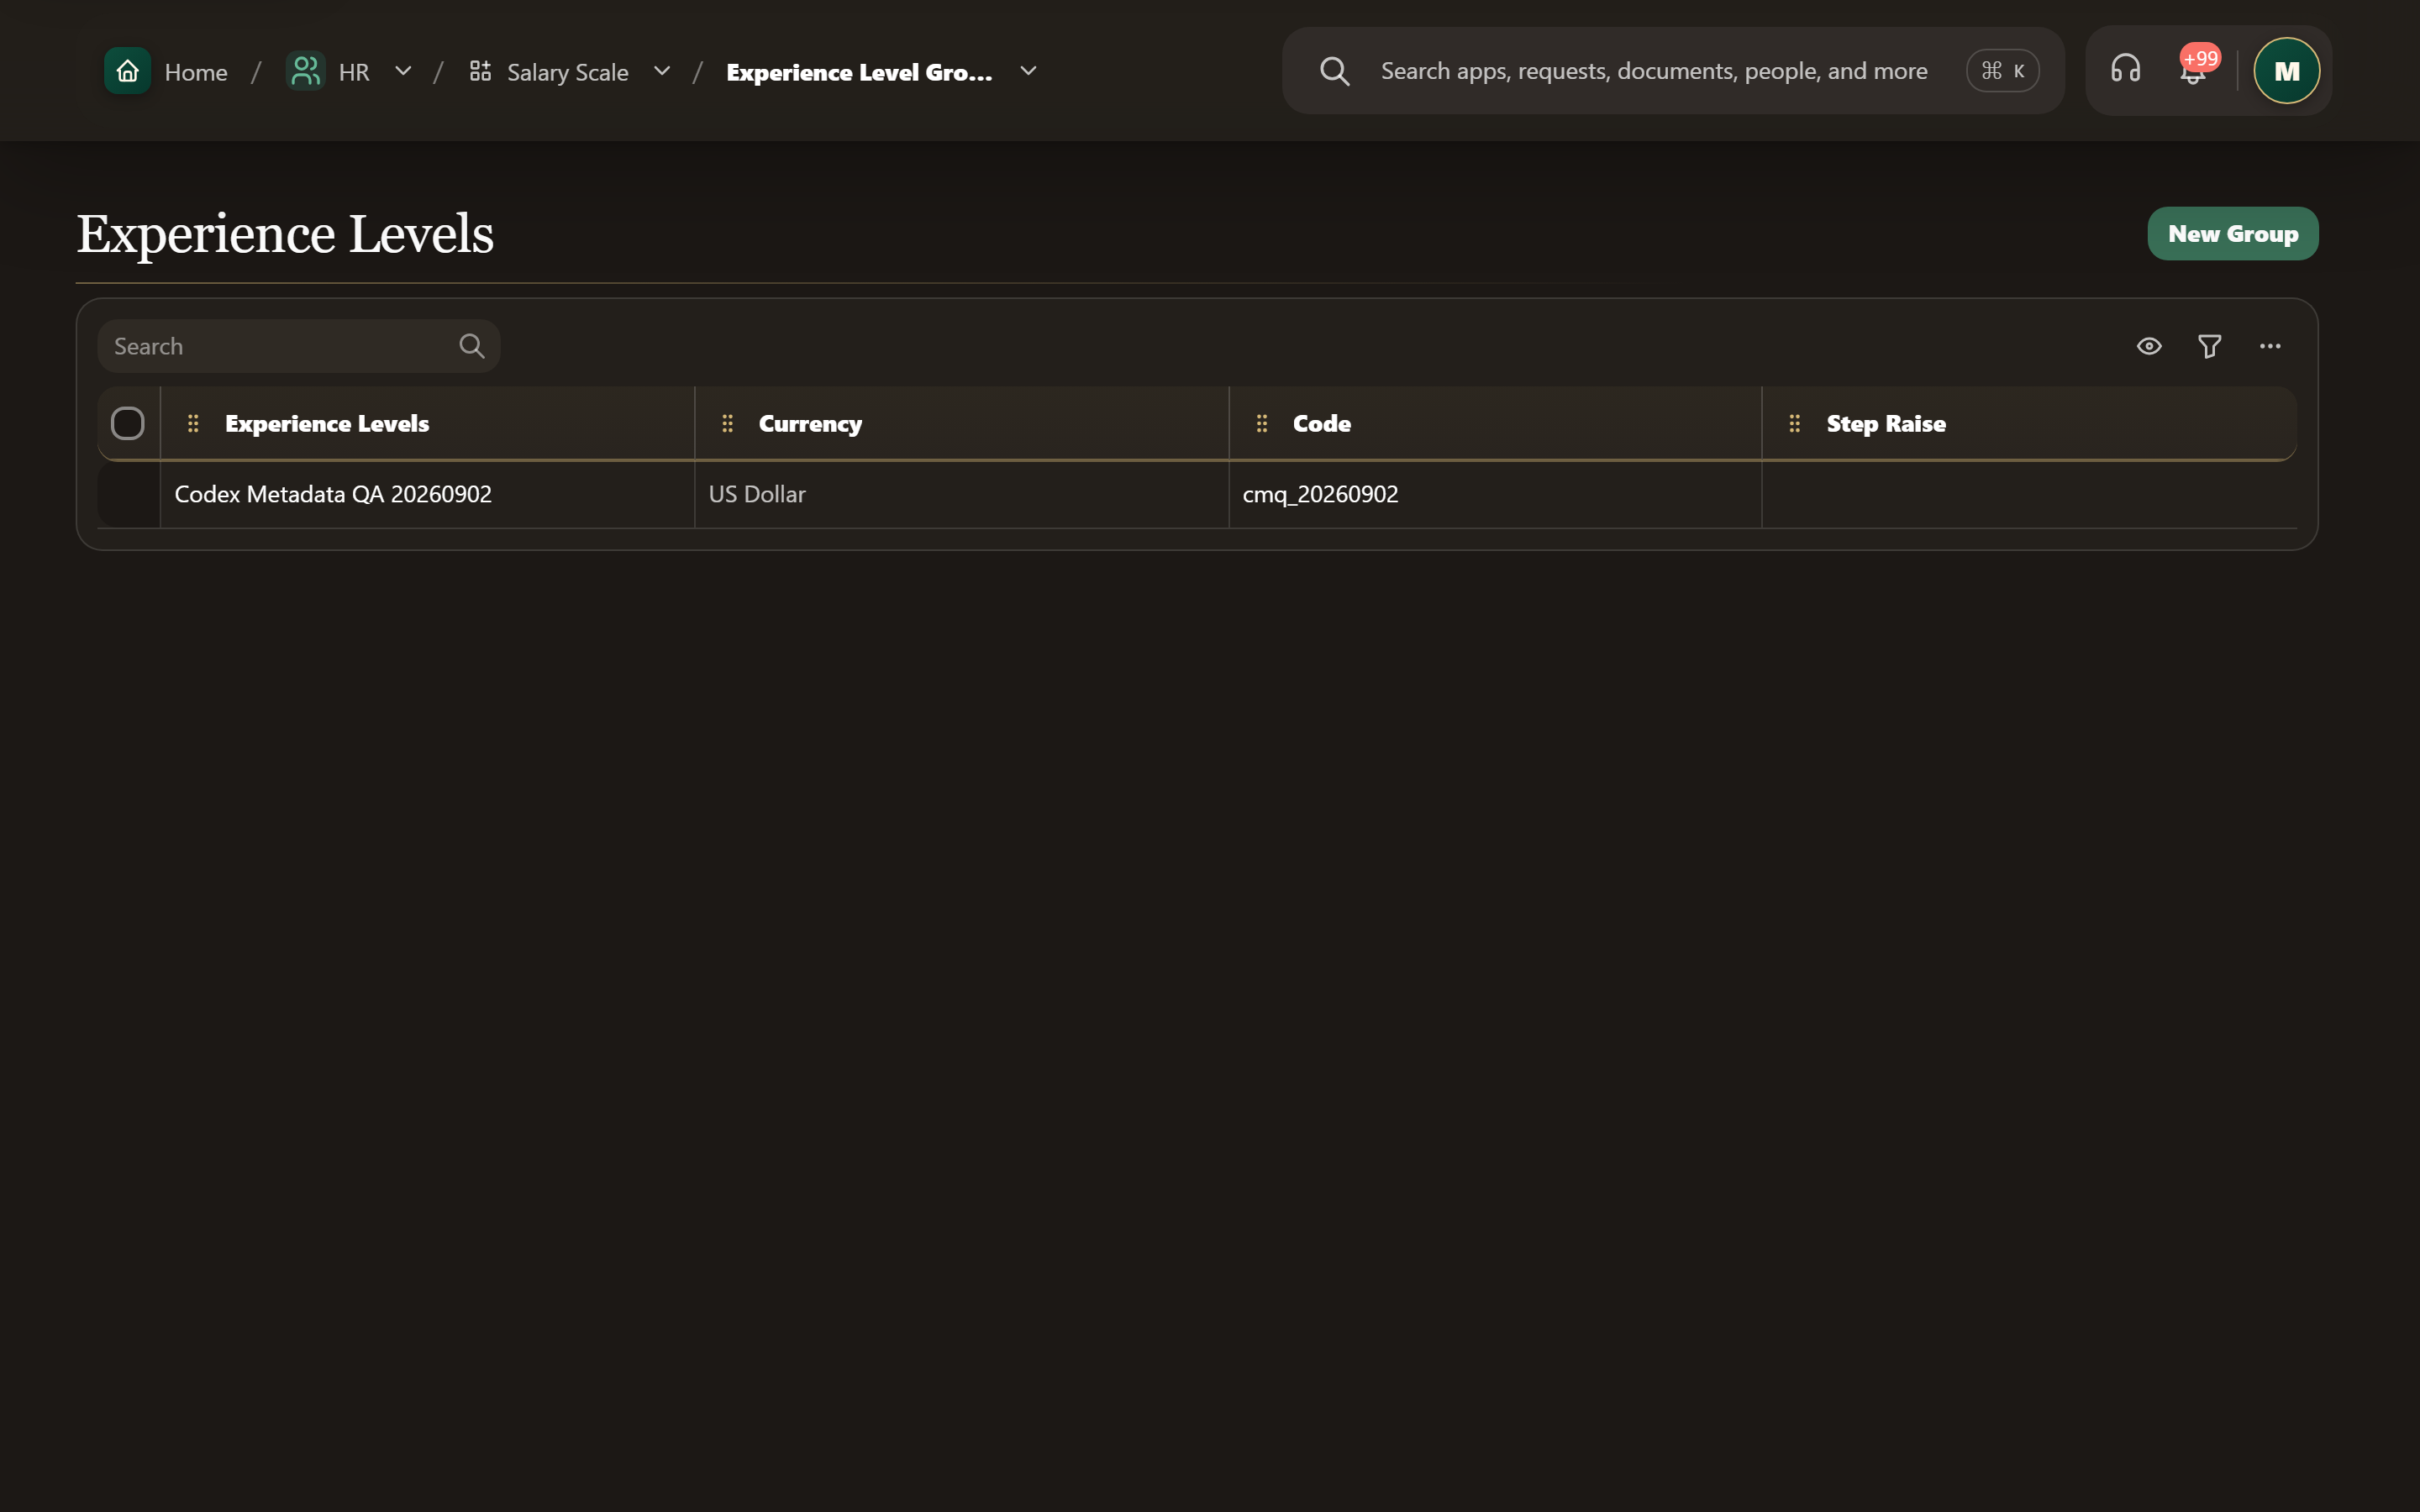
\includegraphics[width=0.95\linewidth]{figures/screens/ch03-feature-experience-levels-en.png}
\caption{Experience Levels: full page in the test environment}
\label{fig:hr-feature-experience-levels-screen}
\end{figure}

\begin{table}[H]
\centering
\caption{What do you record in an experience group?}
\label{tab:hr-feature-experience-levels-data}
\rcZebra
\begin{tabularx}{\linewidth}{R{3.6cm} Y}
\rcHeaderRow
\thh{Tab or field} & \thh{What do you add?}\\
Group & Name, Code and Currency \req{}.\\
Step Raise & “Amount” or “Percentage”.\\
Fixed Raise & When on: one raise per step; otherwise an amount per level.\\
Levels & Name, code and description for each level, ordered by drag and drop.\\
\end{tabularx}
\end{table}

\begin{itemize}
  \item “New Group” and “Add Level”. A level used by assignments cannot be deleted; their list is shown.
\end{itemize}

\begin{figure}[H]
\centering
\begin{tikzpicture}[node distance=0.5cm,stepBox/.append style={minimum width=6.5cm,text width=6.1cm,minimum height=0.8cm}]
  \node[stepBox] (a) {Define the experience group};
  \node[stepBox,below=of a] (b) {Order its levels};
  \node[stepBox,below=of b] (c) {Review the scale};
  \draw[flowsTo] (a) -- (b);
  \draw[flowsTo] (b) -- (c);
\end{tikzpicture}
\rclegend
\caption{Steps of use; arrows do not mean automatic processing}
\label{fig:hr-feature-experience-levels-flow}
\end{figure}

\subsection{Try it and check}

\begin{enumerate}
  \item Open Experience Levels, then “New Group”.
  \item Enter name, code and currency, choose “Amount” and turn on the fixed raise with its amount. Save.
  \item In “Levels” add the levels and order them from least experienced.
\end{enumerate}

\textbf{Check:} open the Salary Scale and review the raises. Do not reorder shared levels to change one person's pay.

\clearpage
\section{Salary Scale}
\label{sec:hr-feature-salary-scale}

The salary scale is a read-only table: a reference salary for each job grade and experience level, calculated from their settings.

\textbf{When is it useful?} Comparing reference pay fairly. The number is a reference, not pay due. \textbf{Open:} HR / Salary Scale / Salary Scale.

\begin{figure}[H]
\centering
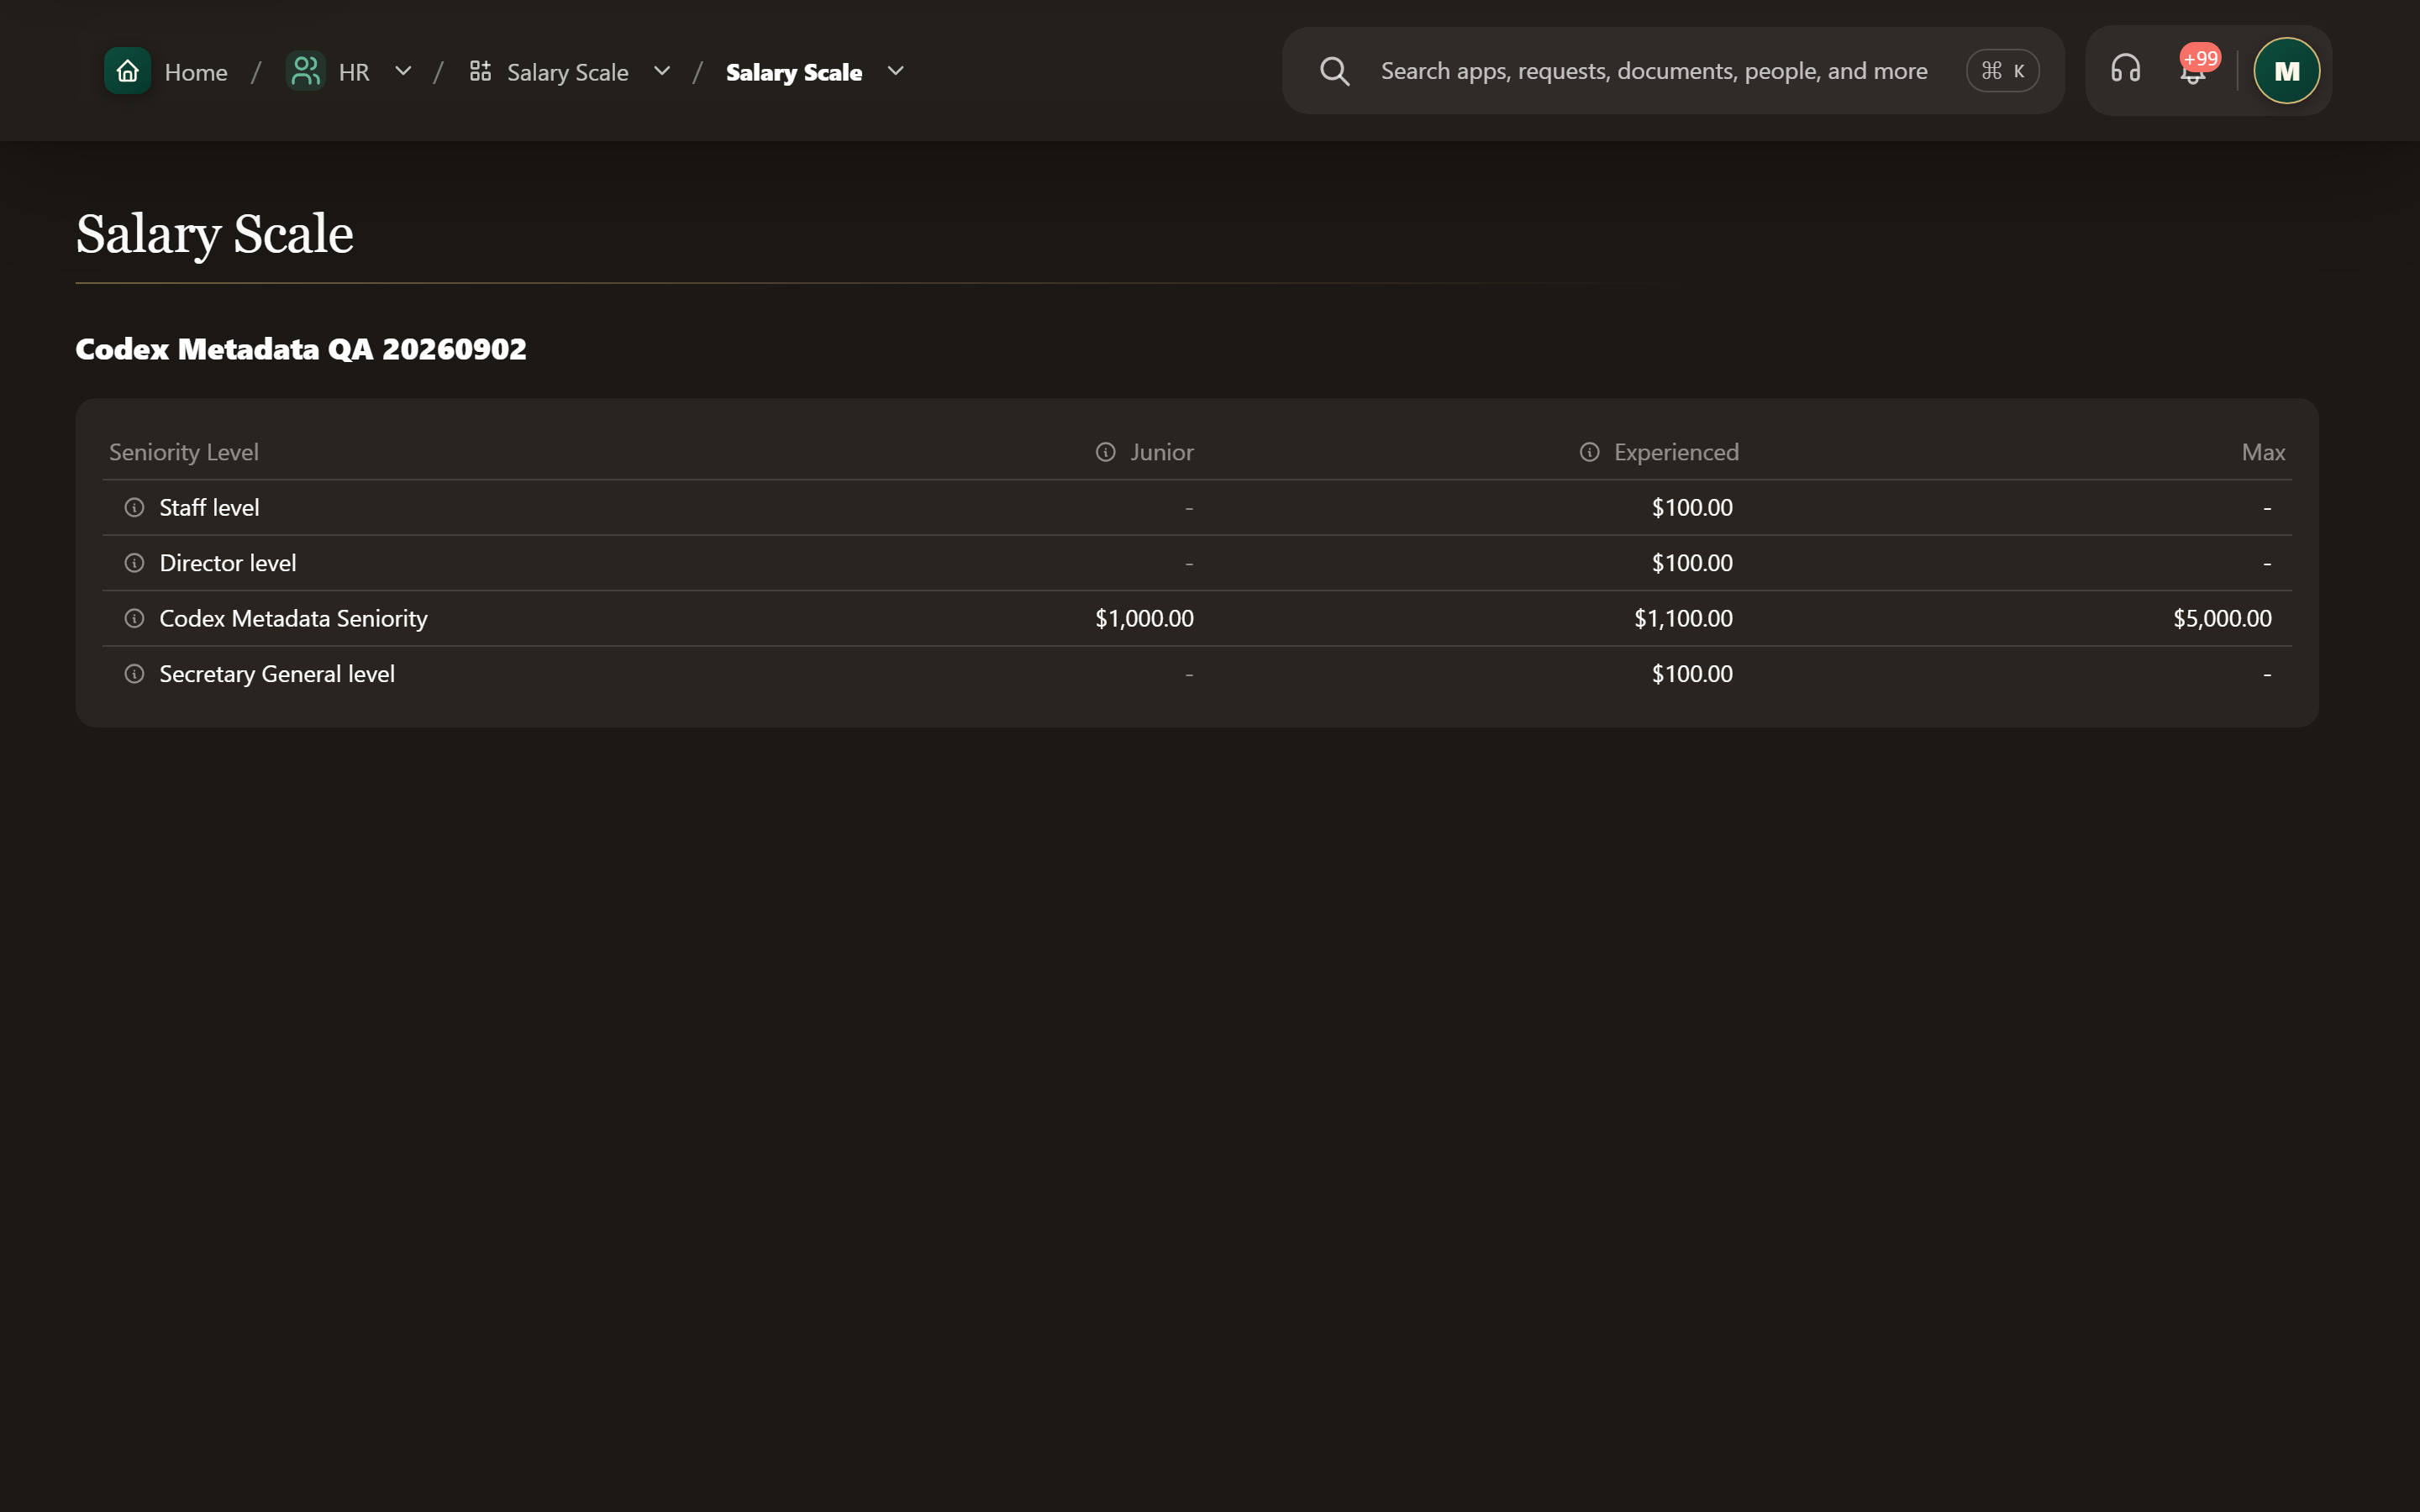
\includegraphics[width=0.95\linewidth]{figures/screens/ch03-feature-salary-scale-en.png}
\caption{Salary Scale: English interface in the test environment}
\label{fig:hr-feature-salary-scale-screen}
\end{figure}

\begin{table}[H]
\centering
\caption{How do you read the salary scale?}
\label{tab:hr-feature-salary-scale-data}
\rcZebra
\begin{tabularx}{\linewidth}{R{3.6cm} Y}
\rcHeaderRow
\thh{Part} & \thh{What does it mean?}\\
One table per group & Each experience group has its own table and currency.\\
Rows & Seniority levels, highest rank first.\\
Columns & Experience levels in order; the last column is the maximum.\\
Cell & The starting salary plus experience raises up to that level \gen{}.\\
\end{tabularx}
\end{table}

The scale is not edited directly; change the seniority levels or experience levels.

\begin{figure}[H]
\centering
\begin{tikzpicture}[node distance=0.4cm,stepBox/.append style={minimum width=6cm,text width=5.6cm,minimum height=0.7cm}]
  \node[stepBox] (s0) {Experience: group and\\increases};
  \node[stepBox,below=of s0] (s1) {Seniority levels: pay\\values};
  \node[stepBox,below=of s1] (s2) {Salary Scale: check\\intersections};
  \node[stepBox,below=of s2] (s3) {Assignment: check pay\\and currency};
  \draw[flowsTo] (s0) -- (s1);
  \draw[flowsTo] (s1) -- (s2);
  \draw[flowsTo] (s2) -- (s3);
\end{tikzpicture}
\rclegend
\caption{If your organization uses a salary scale}
\label{fig:hr-scale-setup}
\end{figure}

\subsection{Try it and check}

\begin{enumerate}
  \item Prepare the experience group and its levels, then the seniority levels. Open the Salary Scale.
  \item Find the grade and experience level and review the cell. If unexpected, check the starting salary and the raise.
\end{enumerate}

\textbf{Check:} compare the reference with Sarah's assignment salary and currency. Arrows show setup order, not automatic payment.

\clearpage
\section{Payroll Inputs}
\label{sec:hr-feature-payroll-inputs}

A payroll input is a variable item for a given month, such as a bonus, deduction or overtime, for an employee's assignment.

\textbf{When is it useful?} Every exceptional amount is recorded and traceable, instead of editing pay by hand. \textbf{Open:} HR / Payment / Payroll Inputs.

\begin{figure}[H]
\centering
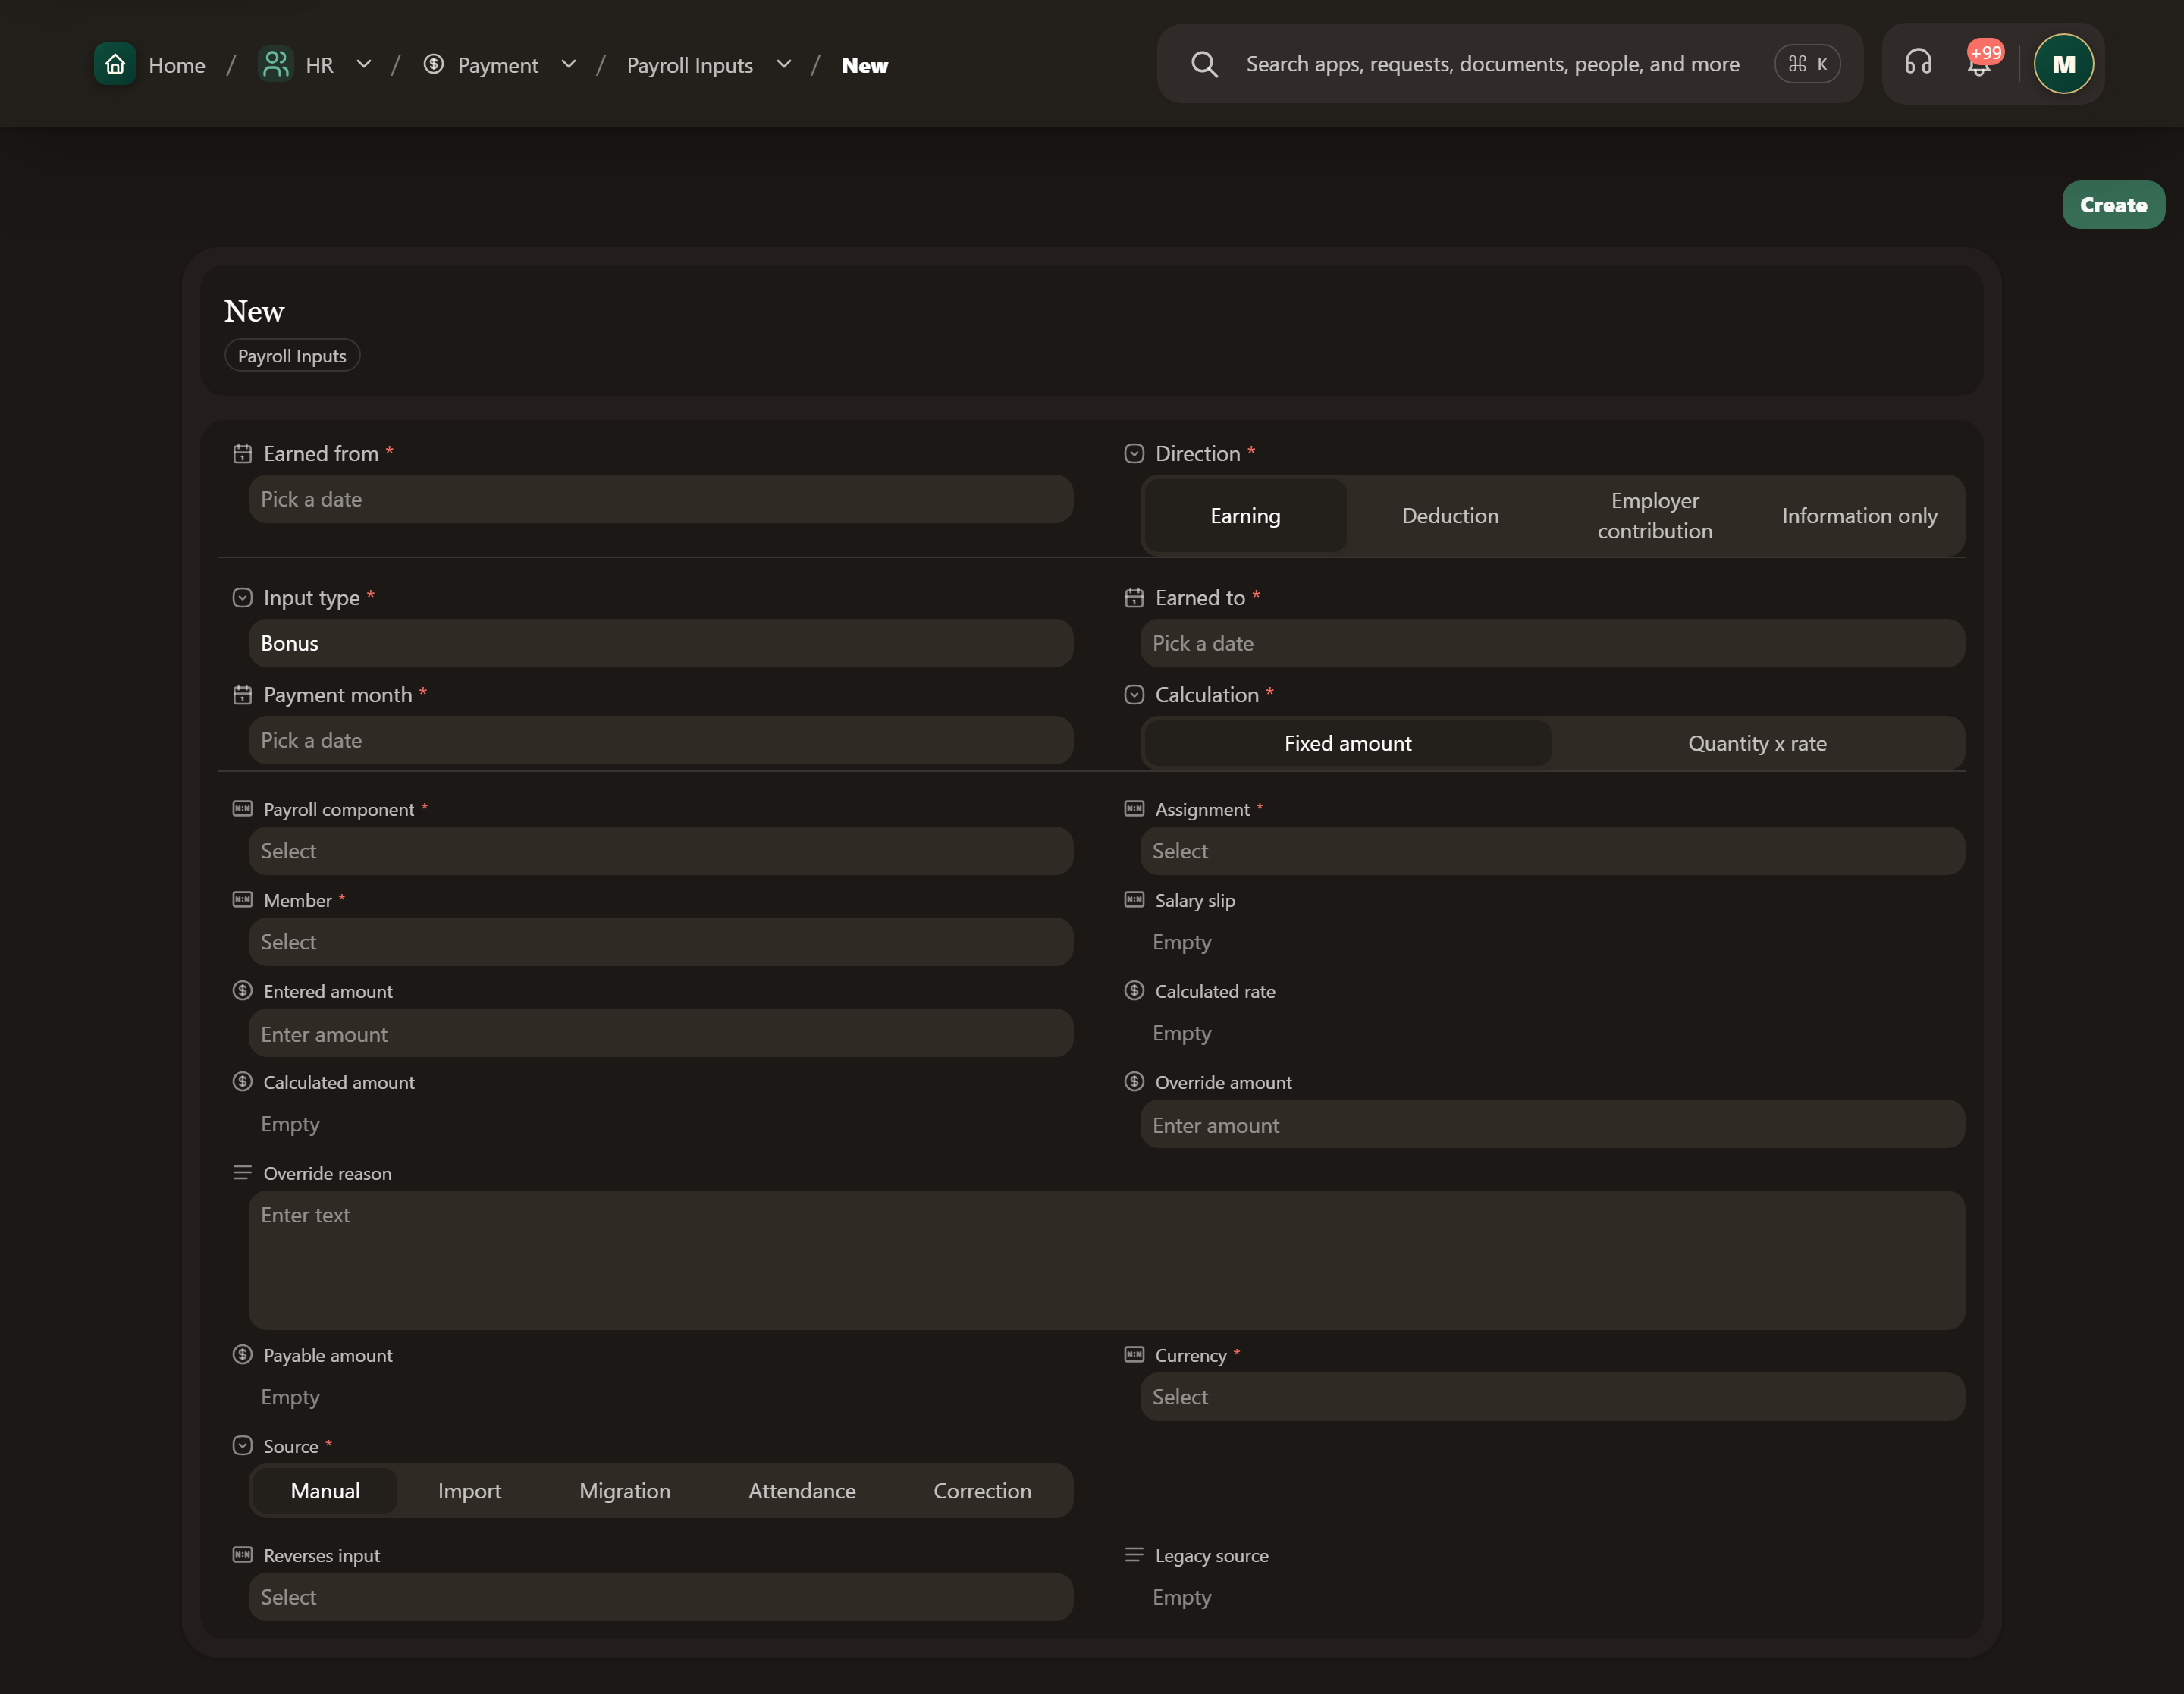
\includegraphics[width=0.95\linewidth]{figures/screens/ch03-payroll-input-fields-en.png}
\caption{Payroll Inputs: complete * fields; not saved}
\label{fig:hr-feature-payroll-inputs-screen}
\end{figure}

\begin{table}[H]
\centering
\caption{What do you record in a payroll input?}
\label{tab:hr-feature-payroll-inputs-data}
\rcZebra
\begin{tabularx}{\linewidth}{R{3.6cm} Y}
\rcHeaderRow
\thh{Field} & \thh{What do you add?}\\
Direction and Input type & \req{}: Earning, Deduction, Employer contribution or Information only; Bonus, Deduction, Overtime, Reimbursement, Correction.\\
Component, Assignment and Member & \req{}: the payroll component, and the same employee's assignment.\\
Period & Earned from and to, and Payment month \req{}.\\
Calculation & Fixed amount, or Quantity x rate; for overtime, hours and time classification: Day, Night, Rest-day, Holiday.\\
Override & Override amount and reason \opt{}.\\
Result & Calculated rate and amount, payable amount and calculation details \gen{}.\\
\end{tabularx}
\end{table}

\subsection{What can you do?}

\begin{itemize}
  \item “Preview calculation” prices the input from the payroll policy and compensation terms.
  \item The input locks once an approved slip uses it. To correct it afterwards, add a new input in “Reverses input”.
\end{itemize}

\begin{figure}[H]
\centering
\begin{tikzpicture}[node distance=0.5cm,stepBox/.append style={minimum width=6.5cm,text width=6.1cm,minimum height=0.8cm}]
  \node[stepBox] (a) {Record the approved item};
  \node[stepBox,below=of a] (b) {Preview its calculation};
  \node[stepBox,below=of b] (c) {Review the salary slip};
  \draw[flowsTo] (a) -- (b);
  \draw[flowsTo] (b) -- (c);
\end{tikzpicture}
\rclegend
\caption{Steps of use; arrows do not mean automatic processing}
\label{fig:hr-feature-payroll-inputs-flow}
\end{figure}

\subsection{Try it and check}

\begin{enumerate}
  \item After reviewing time and leave, open Payroll Inputs and search for the item to avoid duplicates.
  \item Add: “Earning”, “Bonus”, the component, Sarah's assignment, the period and payment month, “Fixed amount” and the approved amount. Save.
  \item Open “Preview calculation” and review the payable amount.
\end{enumerate}

\textbf{Check:} the amount appears in Sarah's slip after “Calculate”. A preview is not a payment.

\clearpage
\section{Salary Slips}
\label{sec:hr-feature-salary-slips}

A salary slip calculates one employee's pay for a period: days, earnings, deductions and net. It moves through stages: draft, calculated, approved.

\textbf{When is it useful?} Review Sarah's own calculation before the payroll, so any amount traces to its item. \textbf{Open:} HR / Payment / Salary Slips.

\begin{figure}[H]
\centering
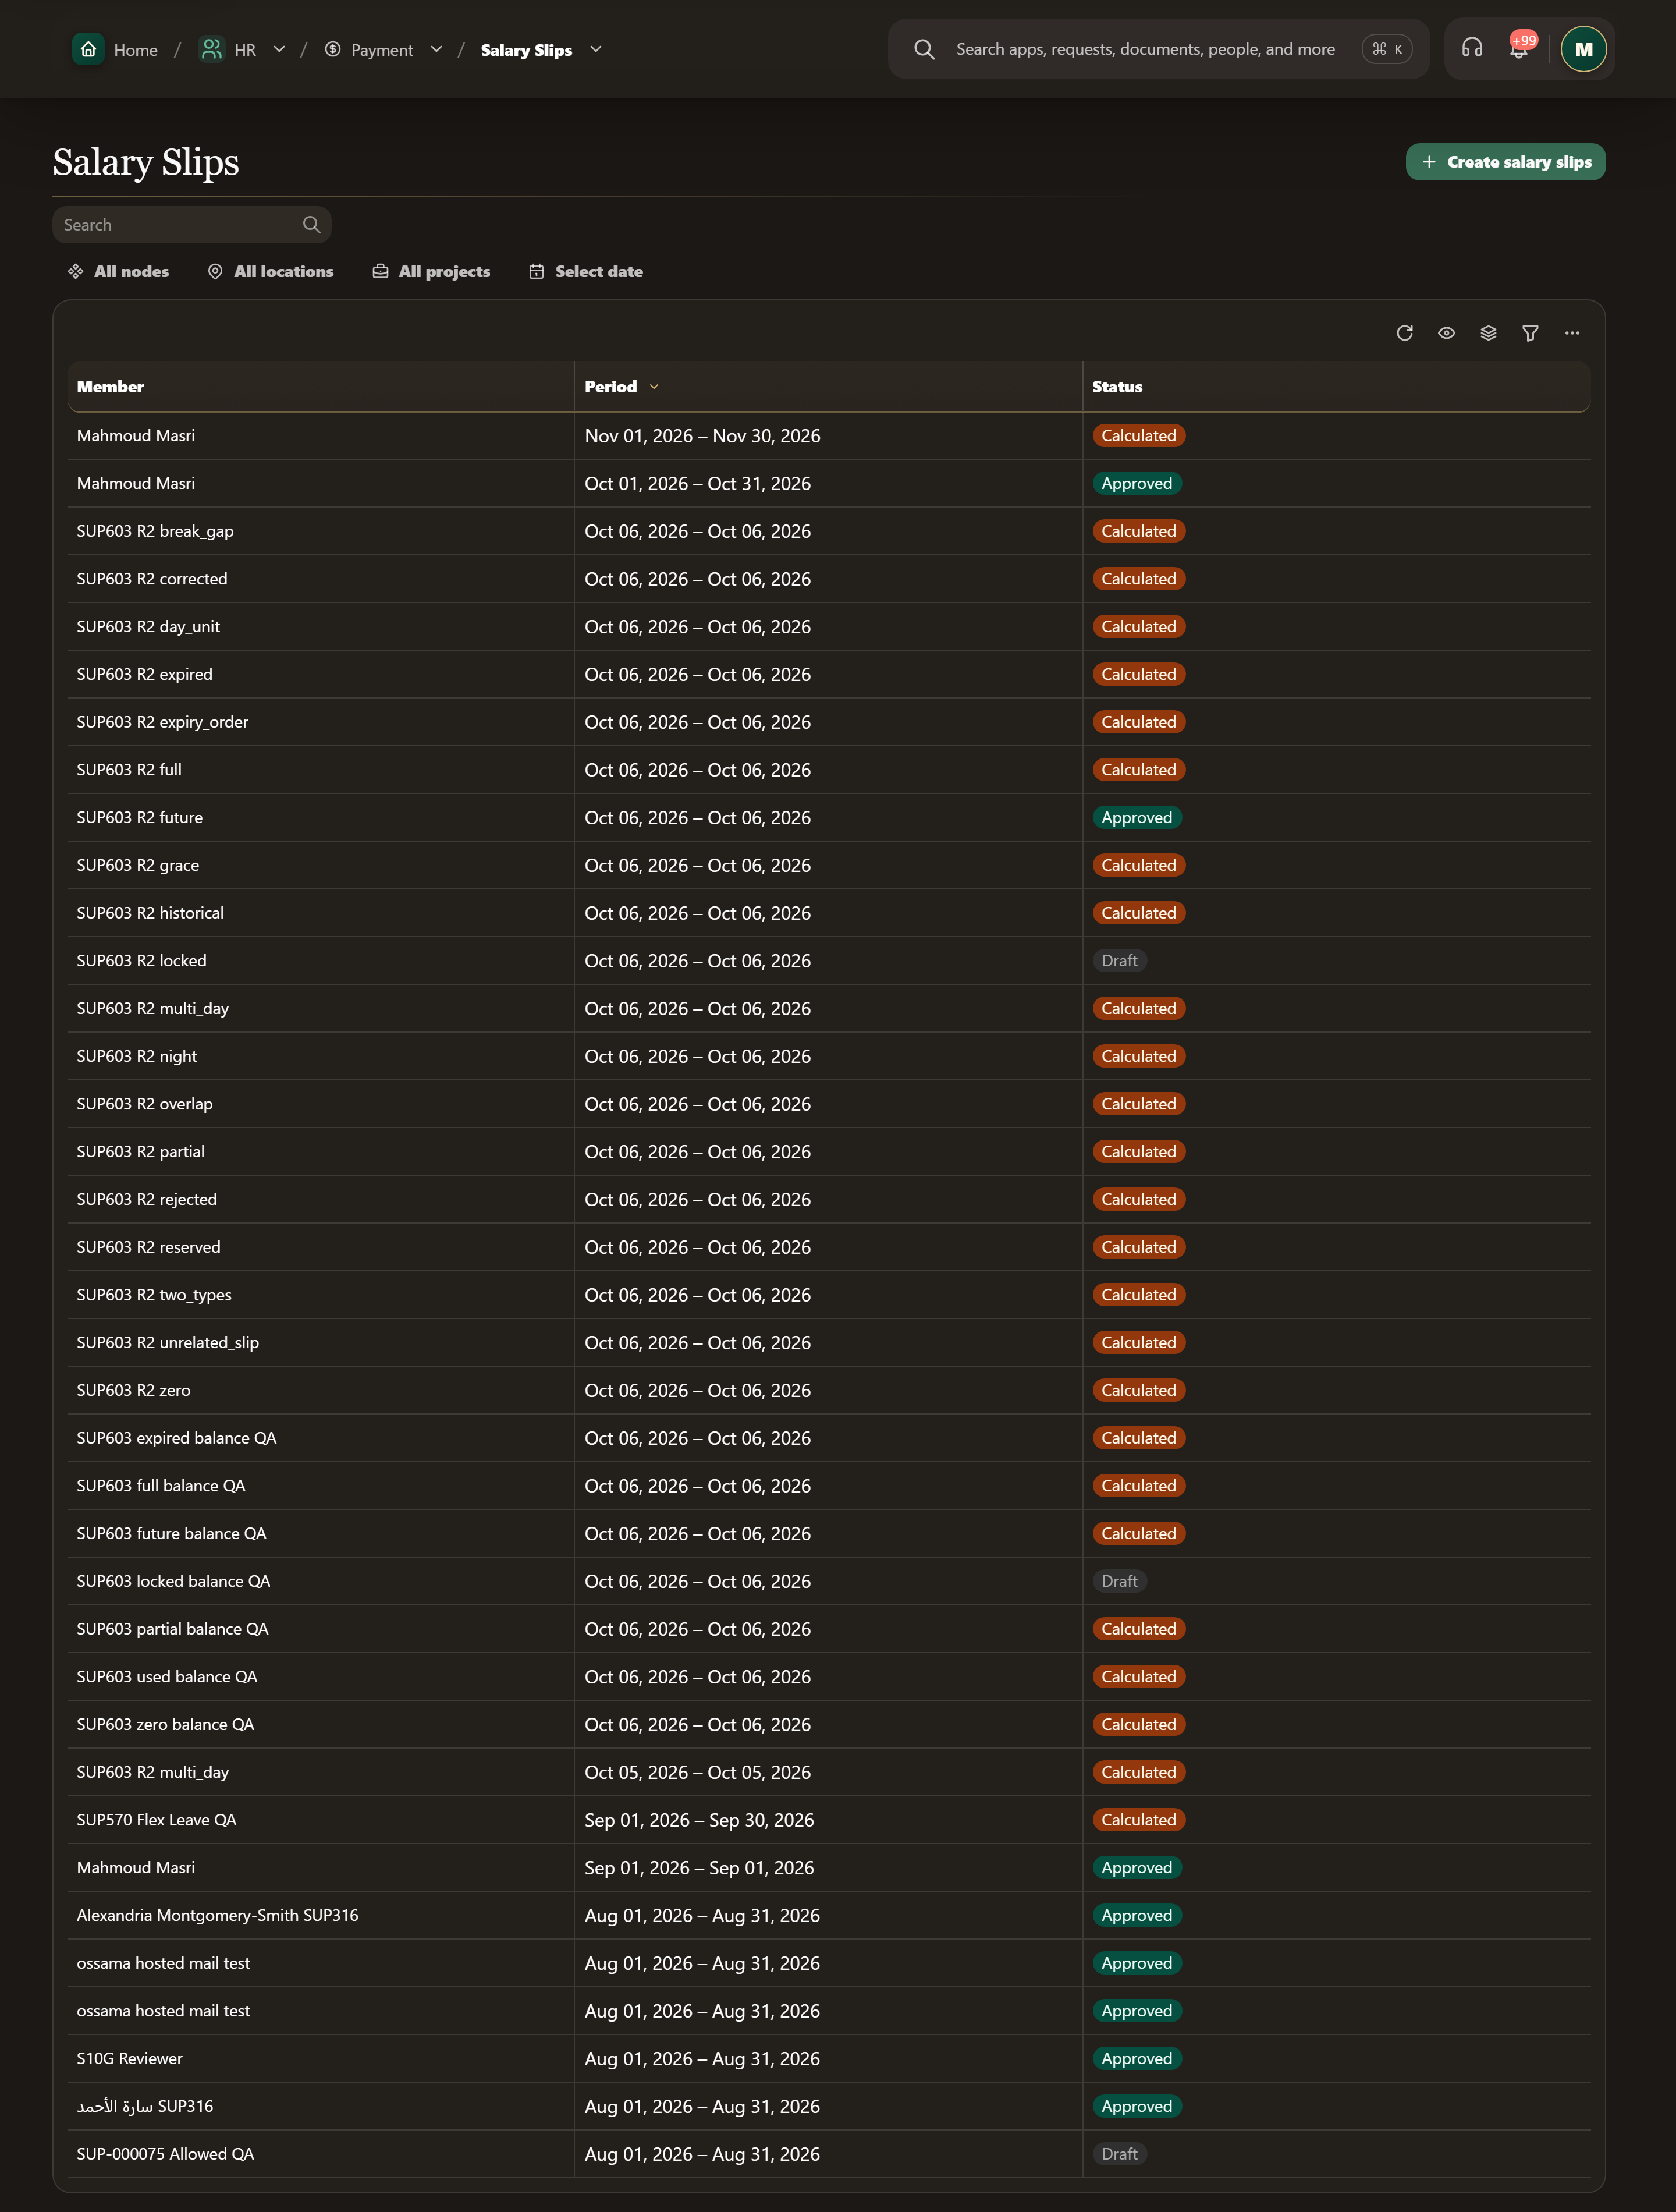
\includegraphics[width=0.95\linewidth]{figures/screens/ch03-create-slips-clear-en.png}
\caption{Salary Slips: full page before creating slips}
\label{fig:hr-feature-salary-slips-screen}
\end{figure}

\begin{table}[H]
\centering
\caption{What does a slip show?}
\label{tab:hr-feature-salary-slips-data}
\rcZebra
\begin{tabularx}{\linewidth}{R{3.6cm} Y}
\rcHeaderRow
\thh{Section} & \thh{What does it show?}\\
Employee information & Name, position, location, contract start and end.\\
Payment summary & Period, work days, currency, base salary for the period.\\
Days & Worked days, holidays, paid and unpaid leaves, overtime.\\
Salary calculation & One line per source with its formula, then amount to be paid, round up and total net salary.\\
Projects and notes & Each project's percentage and amount, and the slip notes.\\
\end{tabularx}
\end{table}

\begin{itemize}
  \item Filter by name, nodes, locations, projects and month.
  \item “Calculate”, then “Recalculate”, “Approve”, and “Delete” for a draft or calculated slip. An approved slip cannot be edited.
\end{itemize}

\begin{figure}[H]
\centering
\begin{tikzpicture}[node distance=0.4cm,stepBox/.append style={minimum width=6.5cm,text width=6.1cm,minimum height=0.7cm}]
  \node[stepBox] (m0) {Assignment and\\employee data};
  \node[stepBox,below=of m0] (m1) {Review time and leaves};
  \node[stepBox,below=of m1] (m2) {Review payroll inputs};
  \node[stepBox,below=of m2] (m3) {Calculate and approve\\salary slip};
  \node[stepBox,below=of m3] (m4) {Generate and review\\payroll};
  \draw[flowsTo] (m0) -- (m1);
  \draw[flowsTo] (m1) -- (m2);
  \draw[flowsTo] (m2) -- (m3);
  \draw[flowsTo] (m3) -- (m4);
\end{tikzpicture}
\rclegend
\caption{Review path from the employee to payroll}
\label{fig:hr-review-flow}
\end{figure}

\subsection{Try it and check}

\begin{enumerate}
  \item Open Salary Slips, then “Create salary slips”.
  \item Choose “Period end”, then Sarah's row and position. Check “Period start”; the first slip starts at the assignment start and can be changed.
  \item Create the draft with the button showing the selected count, then open her slip. If a draft exists, review or delete it instead of duplicating.
  \item Choose “Calculate”. Review the days, lines and net. After changing inputs choose “Recalculate”.
  \item When the lines are correct, choose “Approve” and confirm. Approval consumes the payroll inputs.
\end{enumerate}

\textbf{Check:} the slip status is “Approved” in the list. Approval does not prove payment.

\clearpage
\section{Payrolls}
\label{sec:hr-feature-payrolls}

A payroll gathers a month's approved slips into one sheet, with a total per member and per project.

\textbf{When is it useful?} After checking the slips, to review, approve and export the month's pay. \textbf{Open:} HR / Payment / Payrolls.

\begin{figure}[H]
\centering
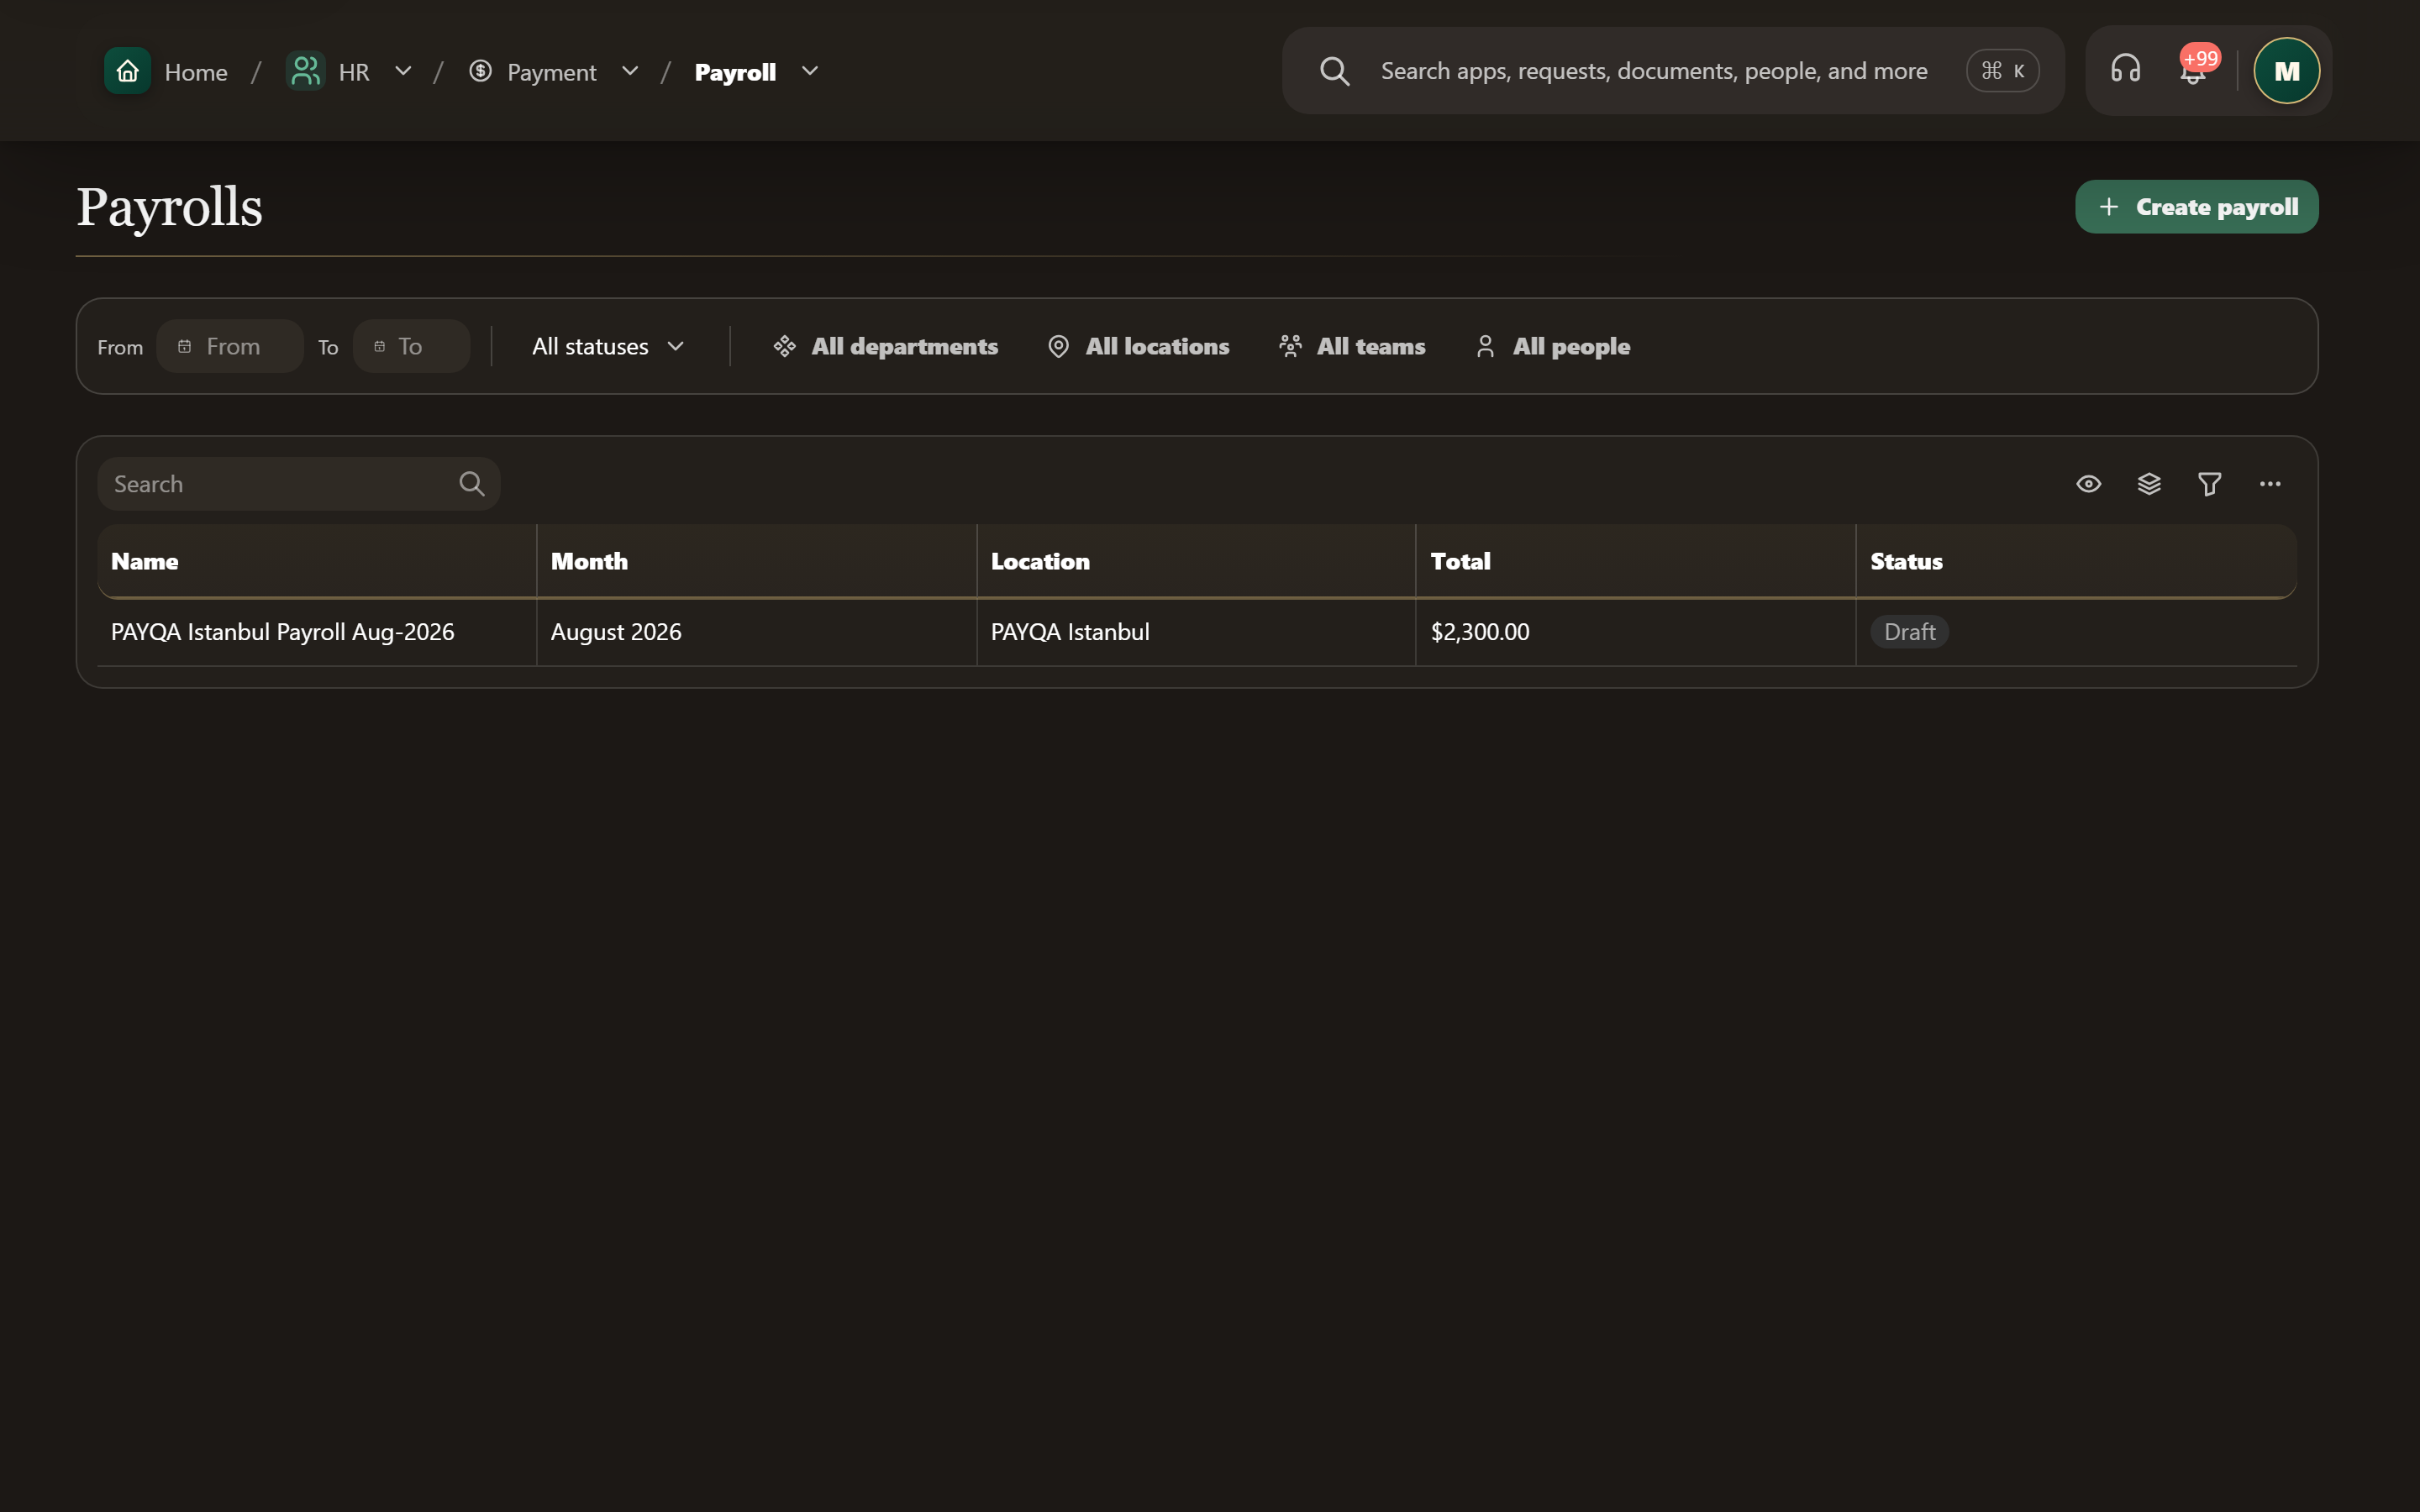
\includegraphics[width=0.95\linewidth]{figures/screens/ch03-feature-payrolls-en.png}
\caption{Payrolls: English interface in the test environment}
\label{fig:hr-feature-payrolls-screen}
\end{figure}

\begin{table}[H]
\centering
\caption{What does a payroll contain?}
\label{tab:hr-feature-payrolls-data}
\rcZebra
\begin{tabularx}{\linewidth}{R{3.6cm} Y}
\rcHeaderRow
\thh{Part} & \thh{What does it show?}\\
Creation & Month and year, approved salary slips or all members, and departments, locations, teams and people.\\
List & Name, month, location, total and status: Draft or Approved.\\
Payments & Per member or per project: working days, rewards, deductions, net salary, amount to be paid, notes.\\
Projects & Each project's percentage and amount, and a total per currency.\\
\end{tabularx}
\end{table}

\begin{itemize}
  \item “Export PDF” for the payroll report, draft or approved.
  \item “Approve payroll” cannot be undone.
\end{itemize}

\begin{figure}[H]
\centering
\begin{tikzpicture}[node distance=0.5cm,stepBox/.append style={minimum width=6.5cm,text width=6.1cm,minimum height=0.8cm}]
  \node[stepBox] (a) {Review approved\\slips};
  \node[stepBox,below=of a] (b) {Generate the period payroll};
  \node[stepBox,below=of b] (c) {Check totals and\\approve the payroll};
  \draw[flowsTo] (a) -- (b);
  \draw[flowsTo] (b) -- (c);
\end{tikzpicture}
\rclegend
\caption{Steps of use; arrows do not mean automatic processing}
\label{fig:hr-feature-payrolls-flow}
\end{figure}

\subsection{Try it and check}

\begin{enumerate}
  \item Open Payrolls, then “Create payroll”. Choose month, year and “Approved salary slips”.
  \item Select the employees and choose “Generate”. If members are already in another payroll, choose “Uncheck members”.
  \item Open the payroll and review the people and total, then “Approve payroll”.
\end{enumerate}

\textbf{Check:} trace each amount to its slip. If an employee is missing, check the month, filters and their slip status.

\begin{rcwarn}[Calculation is not payment]
Approving the payroll only changes its status. Check the transfer and payment records under your organization's procedure.
\end{rcwarn}
